%%%%%%%%%%%%%%%%%%%%%%%%%%%%%%%%%%%%%%%%%%%%%%%%%%%%
%%%     Language Science Press Master File       %%%
%%%         follow the instructions below        %%%
%%%%%%%%%%%%%%%%%%%%%%%%%%%%%%%%%%%%%%%%%%%%%%%%%%%%

% Everything following a % is ignored
% Some lines start with %. Remove the % to include them
% You can skip to line 41

\documentclass[output=book,
%   colorlinks,citecolor=brown
%  ,draft
% ,draftmode,
%  booklanguage=german,
		  ]{langscibook}
%%%%%%%%%%%%%%%%%%%%%%%%%%%%%%%%%%%%%%%%%%%%%%%%%%%%
%%%          additional packages                 %%%
%%%%%%%%%%%%%%%%%%%%%%%%%%%%%%%%%%%%%%%%%%%%%%%%%%%%
\author{Hossep Dolatian}
\title{Adjarian's {\itshape Armenian dialectology} (1911)}
\subtitle{Translation and commentary}

\renewcommand{\lsSeriesNumber}{4}
\renewcommand{\lsSeries}{loc}

\BackBody{Armenian is an Indo-European language that boasts a rich linguistic landscape comprising Classical Armenian (CA), Standard Western Armenian (SWA or WA), Standard Eastern Armenian (SEA or EA), and numerous non-standard dialects, many of which were tragically lost due to the Armenian Genocide. This book is an English translation and commentary of Hratchia Adjarian's seminal work \armenian{Հայ բարբառագիտութիւն} \textit{Armenian dialectology}, originally written in Armenian in 1911. Adjarian describes 31 non-standard Armenian varieties, offering insights into their linguistic structures and historical roots. To enhance accessibility and understanding, this translation unpacks implicit knowledge embedded in Adjarian's text, providing morpheme segmentation, glossing, and translations. This translation is tailored for three distinct audiences: linguists of non-Armenian, traditional Armenian dialectologists, and linguists of Armenian who were trained outside Armenia. This translation aims to bridge linguistic methodologies and facilitate deeper comprehension of Armenian dialectology. The translator supplements Adjarian's prose with commentary, ensuring clarity and accessibility across diverse readerships. This translation provides access to a linguistic landscape of Armenian before the genocide, with the hope of fostering broader scholarly engagement on Armenian dialects.}

\renewcommand{\lsID}{385}
\renewcommand{\lsISBNdigital}{978-3-96110-489-5}
\renewcommand{\lsISBNhardcover}{978-3-98554-118-8}
\BookDOI{10.5281/zenodo.14008766}
\typesetter{Sebastian Nordhoff}
\proofreader{Yasna}

% add all extra packages you need to load to this file

\usepackage{tabularx,multicol}
\usepackage{url}
\urlstyle{same}

\usepackage{listings}
\lstset{basicstyle=\ttfamily,tabsize=2,breaklines=true}

\usepackage{langsci-basic}
\usepackage{langsci-optional}
\usepackage{langsci-lgr}
\usepackage{langsci-osl}
% \usepackage{./langsci/styles/langsci-lgr}
% \usepackage{./langsci/styles/langsci-osl}
% \usepackage{langsci-gb4e}

\usepackage{tikz}
\usetikzlibrary{patterns,calc}
\pgfdeclarepatternformonly{south east lines}{\pgfqpoint{-0pt}{-0pt}}{\pgfqpoint{3pt}{3pt}}{\pgfqpoint{3pt}{3pt}}{
    \pgfsetlinewidth{0.6pt}
    \pgfpathmoveto{\pgfqpoint{0pt}{3pt}}
    \pgfpathlineto{\pgfqpoint{3pt}{0pt}}
    \pgfpathmoveto{\pgfqpoint{.2pt}{-.2pt}}
    \pgfpathlineto{\pgfqpoint{-.2pt}{.2pt}}
    \pgfpathmoveto{\pgfqpoint{3.2pt}{2.8pt}}
    \pgfpathlineto{\pgfqpoint{2.8pt}{3.2pt}}
    \pgfusepath{stroke}}
    
\usepackage{stmaryrd}
\usepackage{wasysym}
\usepackage{multirow}
\usepackage{caption}
\usepackage{subcaption}
\usepackage{mathrsfs}
\usepackage{qtree}

\usepackage{linguex}


%pminos do not split footnotes
% \interfootnotelinepenalty=10000 %Footnote in Laporte chapters has to be split SN


%\DeclareIndexNameFormat{default}{%
%\nameparts{#1}%
%\usebibmacro{index:name}%
%{\index[names]}%
%{\namepartfamily}%
%{\namepartgiveni}%
% {}% L1
% {}% L2
%{\namepartprefix}% generates spurious space L3
%{\namepartsuffix}% generates spurious space L4
%}

%  {\DeclareIndexNameFormat{default}{%
%     \usebibmacro{index:name}{\index[names]}{#1}{#3}{#5}{#7}}}

%\DeclareIndexNameFormat{default}{%
%  \usebibmacro{index:name}{\sindex[nom]}{#1}{#3}{#5}{#7}}

%\DeclareIndexNameFormat{default}{%
%  \usebibmacro{index:name}{\sindex[person]}{#1}{#3}{#5}{#7}}
%\DeclareIndexNameFormat{default}{%
%\nameparts{#1} \usebibmacro{index:name}{\sindex[person]]}{\namepartfamily}{‌​\namepartgiven}{\nam‌​epartprefix}{\namepa‌​rtsuffix}}

%\newcommand{\smiley}{:)}

%\renewbibmacro*{index:name}[5]{%
%\usebibmacro{index:entry}{#1}%
%{\iffieldundef{usera}{}{\thefield{usera}\actualoperator}\mkbibindexname{#2}{#3}{#4}{#5}}}

% \newcommand{\noop}[1]{}

%remove for final
%\overfullrule=1mm

\newcommand{\tobi}[2]}}
\renewcommand{\S}[1]{\tobi{#1}{\textsc{*}}}

% this volume references
% puts: [this volume]
% already defined: \citetv
%\newcommand{\citepv}[1]{(\citeauthor{#1} \citeyear*{#1} [this volume])}
\newcommand{\citealtv}[1]{\citeauthor{#1} \citeyear*{#1} [this volume]}

%parentheses around example number
\newcommand{\pref}[1]{(\ref{#1})}

% in-text examples

\newcommand{\lnex}[1]{\textit{#1}} %target lang word
\newcommand{\lnlit}[1]{(lit.: `#1')} %literal reading
\newcommand{\lnlat}[1]{(#1)} % latinization
\newcommand{\lntrans}[1]{`#1'} %translation
\newcommand{\lnexl}[2]%
{\lnex{#1}{} \lnlat{#2}} % ex with latinization
\newcommand{\lnexlat}[3]{\lnex{#1}{} \lnlat{#2}{} \lntrans{#3}} % ex with latinization and tranl.

%ch01
\newcommand{\co}[1]{\mbox{\textbf{#1}}}

%ch09

\newcommand{\cyrbulg}[1]{\begin{otherlanguage*}{bulgarian}#1\end{otherlanguage*}}


%ch10
\newcommand{\nlp}{{\small NLP}}
\newcommand{\mwe}{{\small MWE}}
\newcommand{\rae}{{\small RAE}}
\newcommand{\lvc}{{\small LVC}}
\newcommand{\pos}{{\small P}o{\small S}}
%\newcommand{\todo}[1]{ \textcolor{red}{#1} }

%\renewcommand{\labelenumi}{\theenumi}
%\ainamefmt{{vv}{ll}{, ff}{, jj}} % fullname

\newcommand{\biberror}[1]{{\color{red}#1}}

\newcommand{\osenovaitem}{--~}
%% hyphenation points for line breaks
%% Normally, automatic hyphenation in LaTeX is very good
%% If a word is mis-hyphenated, add it to this file
%%
%% add information to TeX file before \begin{document} with:
%% %% hyphenation points for line breaks
%% Normally, automatic hyphenation in LaTeX is very good
%% If a word is mis-hyphenated, add it to this file
%%
%% add information to TeX file before \begin{document} with:
%% %% hyphenation points for line breaks
%% Normally, automatic hyphenation in LaTeX is very good
%% If a word is mis-hyphenated, add it to this file
%%
%% add information to TeX file before \begin{document} with:
%% \include{localhyphenation}
\hyphenation{
    Beck-man
    Ngu-yen
    back-chan-nel
    back-chan-nels
    mo-not-o-nous
    ste-reo-typ-i-cal
}

\hyphenation{
    Beck-man
    Ngu-yen
    back-chan-nel
    back-chan-nels
    mo-not-o-nous
    ste-reo-typ-i-cal
}

\hyphenation{
    Beck-man
    Ngu-yen
    back-chan-nel
    back-chan-nels
    mo-not-o-nous
    ste-reo-typ-i-cal
}

\addbibresource{localbibliography.bib}

%%%%%%%%%%%%%%%%%%%%%%%%%%%%%%%%%%%%%%%%%%%%%%%%%%%%
%%%             Frontmatter                      %%%
%%%%%%%%%%%%%%%%%%%%%%%%%%%%%%%%%%%%%%%%%%%%%%%%%%%%

\begin{document}
\maketitle
\frontmatter

{\sloppy\tableofcontents}

\addchap{Dedication}

This book is dedicated to the loving memory of Maurice Sarfati (1947–2018) and Ezra Yitzhak Nawi (1952–2021), two dear friends, inspiring critical thinkers and true Jerusalemite legends, who passed away while I was working on this research.

\addchap{\lsAcknowledgementTitle} 

\textit{Núu'etaa numá'kaaki wáakapusmak wakápusa wakų́'ro'sh}. 

This book would not have been possible without the generosity and foresight of various Mandan speakers who gave their time and energy into recording their language and their knowledge. Some of the key Mandan individuals who have provided to this corpus, which extends back over a century and a half, include: Mrs. James Kipp (a.k.a., Earth Woman), Mrs. Holding Eagle (a.k.a., Scatter Corn), Mr. Ben Benson (a.k.a., Buffalo Bull Head), Mr. Flat Bear (a.k.a., Bear on the Flat), Mr. Walter Face (a.k.a., Wounded Face), Mrs. Little Crow (a.k.a., Otter Woman), Mr. Paul Crows Heart (a.k.a., Crows Heart), Mr. Sitting Rabbit, Mr. Little Crow, Mr. Wolfs Head, Mr. Wolf Ghost, Mr. White Calf, Mr. Foolish Woman, Mr. Little Owl, Mrs. Good Bear, Mrs. Calf Woman, Mrs. Owen Baker, Mrs. Front Woman, Mr. Wolf Chief, Mrs. White Duck, Mrs. Edna Face, Mrs. Nora Baker, Mr. Stephen Bird, Mr. Mark Mato, Mrs. Bessie Medicine Stone, Mrs. Mary Atkins, Mrs. Blanche Benson, Mr. Burr Crows Breast, Mrs. Annie Eagle, Mrs. Mattie Grinnell, Mr. Albert Little Owl, Mr. Ralph Little Owl, Mrs. Otter Sage, Mr. John Stone, Mr. Clyde Baker, Mr. Jacob, Bird, Mr. William Bell, Mrs. Louella Benson Young Bear, Mr. Ernest Medicine Stone, Mr. Carl Whitman, Ms. Ann Solano, Mr. Leon Little Owl, Mr. Corey Spotted Bear, and Mr. Edwin Benson.

I also gratefully acknowledge that I was able to assemble the materials and information found in this book over the years thanks to the generous financial support of the American Philosophical Society's Phillips Fund for Native American Research, Yale University's A. Richard Diebold Jr. Graduate Fellowship and the Frederick W. Hilles Memorial Scholarship Fellowship, Northeastern Illinois University's Dr. Bernard J. Brommel Doctoral Scholarship, and freelance employment by the Language Conservancy through its contract with the Mandan-Hidatsa-Arikara Nation's Department of Education. I also could never have completed this book without the support provided to me by my employer, the University of Oklahoma, where I had been afforded a semester of teaching release after my third year to ensure that this book could be completed.

My long-time advisor at Yale, Prof. Stephen Anderson, saw many early versions of papers and projects that led to what is now this book. His guidance was instrumental to the theoretical conclusions I made in my dissertation, and that dissertation formed the backbone of the present monograph. Prof. Claire Bowern, my other dissertation co-chair and professor was likewise key to my ability to complete my dissertation, especially after I left New Haven and worked on my dissertation \textit{in absentia} for several years. She held me accountable to making progress, and I deeply appreciate the time and energy she spent in getting me across the finish line. Prof. Natalie Weber, a dissertation committee member, looked over many versions of the analyses that became the chapter on Mandan phonetics and phonology in this book. I am grateful for their time in walking me through more effective ways of presenting the data there. Prof. Marianne Mithun, as a member of my dissertation committee, provided valuable insight into how different processes in Mandan worked and how they fit into the typology of North American languages. Her own experience in studying Siouan languages and her breadth of knowledge on language change improved how I presented the morphological data in what has become the verbal morphology chapter of this book.

On a more personal level, my parents Raymond and Kathleen Kasak have contributed to much to the evolution of this book by asking me repeatedly over the years, ``is it done yet?'' Since the spring of 2015, many phone conversations ended with a question as to the status of this work. First, they asked when I was working on my dissertation, which this book uses as a launchpad for a more comprehensive grammar. Later, as I was preparing this manuscript for submission to Language Science Press, they would ask me whether I was done with this chapter or that chapter yet. Any academic surely understands how incredibly welcome and not at all stressful such questions were.

The friends I made at my M.A in Linguistics at Northeastern Illinois University helped get me to Yale and were, therefore, important to getting this book finished. Dr. John Boyle, first as my professor and then as my friend, introduced me to Siouan linguistics, so I could not have even begun to build the foundations of this book without him. I am thankful for him taking me to my first Siouan and Caddoan Languages Conference in Kansas and him introducing me to the late, great Bob Rankin, one of the monumental figures of Siouan linguistics. My former professors Drs. Shahrzad Mahootian and Lewis Gebhart were great moral support in convincing me to apply to grad school and checked in with me often to see how things were going. My former NEIU classmates Dr. Binh Ngo and Galini Gkartzonika have likewise been great friends and supporters throughout my time at Yale and beyond. I also could not have written this book without the editorial assistance of my wonderful friend Hadley Austin and my former student Lizz Evalen, whose proofreading of an earlier version of my dissertation has made the writing of this book much easier.

My final and most important acknowledgment goes to my partner and wife Dr. Colbi Beam, who has been a singular source of inspiration to complete this work. I am forever grateful for her love and support. I have no doubt that this book would have taken far longer to complete without her encouragement and her understanding of what it takes to write academically. Having written a dissertation herself, she understood the nature of writing expansive pieces of work and she was helpful in putting aspects of the writing process in perspective for me during times when I struggled with how to present some data or was unsure how to best resolve some impasse in writing. She has been insightful and inspirational throughout this process. Colbi, you are simply the best.
% % % % \addchap{Preface}

This book has had a rather long gestation period. The papers in this collective volume originate in
a selection of the papers that were presented at a workshop at Freie Universität Berlin in May
2017, which was jointly organised by Ulrike Freywald, then University of Potsdam, and Horst Simon,
FU Berlin. In an elaborate and anonymous peer review process, the papers were selected and revised
under the guidance of UF and HS, and finally refined and brought into their present shape by Stefan
Müller, who had also presented at the workshop, and his team at HU Berlin. 

We thank various institutions and individuals, above all the Deutsche Forschungsgemeinschaft and the
Ernst-Reuter-Gesellschaft der Freunde, Förderer und Ehemaligen der Freien Universität Berlin
e.V. for their financial support of the workshop, then a host of colleagues, who need to remain
anonymous, who have offered their expertise when peer reviewing, and finally a group of student
assistants in the final process of polishing the papers into publishable form, namely Elisabeth
Eberle, Luisa Kalvelage, and Julie Täge.

It is to be hoped that the present volume will testify more to the potential headlessness of the
structures discussed than to the headlessness of the pondering linguist. 

\bigskip
\noindent
Berlin \& Dortmund, \today \hfill \begin{tabular}[t]{@{}r@{}}
                                  Ulrike Freywald\\
                                  Horst J.\ Simon \\
                                  Stefan Müller
                                  \end{tabular}






 \mainmatter

%%%%%%%%%%%%%%%%%%%%%%%%%%%%%%%%%%%%%%%%%%%%%%%%%%%%
%%%             Chapters                         %%%
%%%%%%%%%%%%%%%%%%%%%%%%%%%%%%%%%%%%%%%%%%%%%%%%%%%%

\part{Introduction}
 \chapter{General introduction}\label{sec:genIntro}

\section{The sonority challenge}\label{the-sonority-challenge}\largerpage[2]

%Various speech researchers -- the author of this book included -- have often been displeased with the state of affairs regarding the notion of \emph{sonority} as it is conventionally used in phonetics and phonology.
Sonority is a central notion in phonetics and phonology, with many useful formal applications, yet it has remained vague in too many important respects.
The centrality of sonority is primarily derived from the important theoretical weight that it carries in descriptions of syllables in phonology. Sonority is a single hierarchical concept that is most often used to characterize all speech sounds along a single scale in a manner that is pivotal for generalizing preferences and restrictions on syllabic organization.

However, even after many decades in which sonority has played a crucial role in phonology, there is no consensus with regards to its \emph{phonetic} basis in articulation or perception of speech. Many proposals have been debated, but no real consensus has ever been reached.
Sonority therefore presents an ongoing phonetic challenge.
A good overview of the multiplicity of proposals for the basis of sonority can be found in the various publications by Stephen Parker, from his dissertation \citep{parker2002quantifying}, to subsequent publications \citep[like][]{Parker:TheSonorityControversy:2012, parker2017sounding, parker2018abib} that meticulously document the vast research related to sonority in the linguistic literature.

The most prevalent models of sonority are based on the \emph{Sonority Sequencing Principle} (SSP) and they are very characteristic of linguistic models from the second half of the twentieth century, whereby the speech signal is represented as a sequence of discrete units, phonological processes are modeled as symbol manipulating rules, and time is accounted for in terms of the non-overlapping linear order of the discrete units in symbolic representations (see \sectref{sec:risenfall}).

It may very well be the case that little progress has been made in the theory of sonority since the turn of the century because of the constraining role that SSP-based models play with regards to phonetic dimensions. Specifically, the classic theoretical idea that the speech signal is composed of segments that have a fixed sonority value, which they share with other members of the same category, may have created an impossibility in the traditional theory. This is because the speech signal does not in fact lend itself to such analyses of non-overlapping discrete units with fixed sonority values (see \sectref{sec:risenfall}). Such units can only be extracted from a human mind. In other words, the classic theory may have created a formal notion of sonority that simply cannot be found in any phonetic space.

The challenges of sonority are therefore at the intersection of phonetics and phonology.
Chiefly, these are issues pertaining to phonetic substance itself and to phonological theory, which accounts for the parts of the system that are linguistically relevant.
A better model of sonority would seem to require novelties on both fronts.

\section{Beyond correlates}\label{beyond-correlates}

Another issue highlighted by the notion of sonority, and directly related to the above, is the lack of explanatory power in many phonological models.
A good example of this problem can be gleaned from the common practice of suggesting acoustic \emph{correlates} for various linguistic phenomena, without any related attempt to suggest plausible \emph{causation}. This is very often the case when the suggested acoustic correlates do not seem to have any clear and consistent links to the perception or articulation of speech.
In many other cases, the implied causation can be misguided.
A case in point is the use of physical acoustic intensity as a correlate of linguistic phenomena -- sonority \emph{inter alia} -- although the physical amplitude of the entire signal does not consistently relate to perceived loudness, or any other aspect of perception and/or articulation (see details in Section~\ref{sec:correlusions}).

Thus, it seems already at the outset of this project that in order to suggest a form of phonetic substance for sonority we need to be able to explain its function in the language system, beyond its ability to exhibit statistical correlations with sonority hierarchies. This cannot be achieved with a few tweaks in traditional discrete and symbolic models, as they are too far removed from cognitive plausibility owing to their classic computer-like architectures (see \chapref{sec:lingMod}).
The mainstream models of phonology from the second half of the twentieth century are simply not designed to achieve explanatory goals of this kind.

\section{Goals and motivations of the current endeavor}\label{goals-and-motivations-of-the-current-endeavor}

The challenges that sonority presents are far-reaching, as apparent from the list of problems detailed above. Solving them requires a host of theoretical and methodological novelties that necessitate a relatively large-scale effort.
%, such as this book-length project.
To undertake these challenges, this work aims to determine what sonority \emph{is}, what it \emph{does}, and \emph{how} it does it. To this end, it is also imperative to break away from traditional discrete and symbolic models in linguistics by incorporating continuity and dynamics in a perception-based model of phonology.

%If proven successful, the fruits of this endeavor will also be far-reaching, beyond the specific treatment of sonority. This immediately includes new approaches to the study of prosody, where sonority plays a crucial role.
%Moreover and more generally, this includes new approaches to perception-based models in phonology, suggesting a more principled way to exploit acoustic data in linguistic research.
%Lastly, this endeavor can contribute even more generally to a growing need for new approaches to modeling linguistic systems with both discrete and continuous entities that can coexist and interact in a complementary way.


\section{A note about terminological choices}\label{a-note-about-terminological-choices}

Terminology can be confusing.
Often there are multiple terms for the same thing, and they are sometimes loaded with differing implications in different scientific and professional circles.
The following description of terminological interpretations is intended to reduce confusion for readers of this book.

The terms \textsc{consonant} and \textsc{vowel} are used here broadly to denote the phonological entities, which also consider the position within the syllable. In some cases, when it is specifically relevant to only refer to phonetic features (i.e.~only to the degree of vocal tract stricture), I use the terms \textsc{contoid} and \textsc{vocoid} (respectively), following \citet{pike1943phonetics}.

Successive consonants that follow each other in the phonological description are either referred to as a \textsc{sequence} or a \textsc{cluster}. The latter has a more specific meaning, implying that \emph{clusters} are syllabified together in a single syllable, thus constituting a tautosyllabic complex onset or coda. The term \emph{sequence} is used when no implication is made about the status of the two successive items, which could also be heterosyllabic.

When writing about auditory perception, it can be useful to keep acoustic and perceptual aspects separate via distinct terminology. The terms \textsc{intensity}, \textsc{power} and \textsc{amplitude} relate to the acoustic signal. They are often interchangeable although whenever the distinction between the raw pressure and the log-transformed dB scale is relevant, I use \emph{power} for the raw pressure and \emph{intensity} for the the log-transformed dB scale. Crucially, the related term for perception of acoustic strength is consistently \textsc{loudness}.
Likewise, F0, or the \textsc{fundamental frequency}, always refer to the acoustic signal. The related term in perception is \textsc{pitch}.

Note that the terms \textsc{tone} and \textsc{tune} have specific meanings in linguist contexts. A tone is a pitch target with a communicative function that is either part of the lexical repertoire (e.g.~\emph{lexical tone}) or the post-lexical repertoire (e.g.~a \emph{pitch accent}/\emph{boundary} tone). A \emph{tune} is often used to describe larger intonation contours (that are commonly analyzed as being composed of tones).

This book deals with \textsc{discrete} vs.~\textsc{continuous}, and with \textsc{symbolic} vs.~\textsc{dynamic} entities or elements. These pairs are interchangeable in the majority of the contexts used here.
Likewise, the terms \textsc{trajectory} and \textsc{curve}, as they are used here to denote graphs within plots or, more abstractly, when describing the progression of a certain feature in time, are largely interchangeable.

%\subsection{Other technical notes}\label{other-technical-notes}

\section{Conventions}\label{conventions}

Phonemic depictions of speech are presented in this book with mostly standard IPA conventions. A few diversions from the IPA norm include the use of acute accents (´) on the vowel (e.g.~é, ó, á) to mark the stressed syllable, and the use of the simple grapheme /c/ to denote the voiceless alveolar affricate, which is transcribed with the complex grapheme /t͡s/ in the standard IPA.

Within phonemic transcriptions, a dash (-) is sometimes used to mark morpheme boundaries, while a dot (.) is used to mark syllabic boundaries. For instance, \emph{dla.t-ót} stands for `door-\Pl{}' in Modern Hebrew, where the suffix \emph{-ot} forms a syllable with the final consonant of the base morpheme (/t/), as shown by the
location of the dot.

%	\subsubsection{Methods}\label{methods}
%	
%	This thesis was written with \emph{RStudio} (\citet{rstudio}), using the following packages to combine text and code in a single file that can output LaTeX documents with APA style: R (Version 3.6.3; R Core Team, 2018) and the R-packages \emph{knitr} (Version 1.28; Xie, 2020), \emph{papaja} (Version 0.1.0.9942; Aust \& Barth, 2020), and \emph{rmarkdown} (Version 2.2; Allaire et al., 2020).

\section{Scope of book}\label{scope-of-book}

The current book is divided into five parts in an attempt to address all the necessary issues mentioned above. The first part, \emph{Introduction}, includes this chapter (\chapref{sec:genIntro}) and two more chapters that present the relevant background on sonority (\chapref{sec:background}) and linguistic models more generally (\chapref{sec:lingMod}).

The second part, \emph{Novel theoretical outlooks}, contains three chapters that present the new theoretical proposals that this work develops:
(i) the PRiORS framework for modeling auditory perception (\chapref{sec:priors});
(ii) the proposal for sonority's perceptual cause and acoustic correlate, and the new sonority-based criterion for well-formedness determinations, the \emph{Nucleus Attraction Principle} (\chapref{sec:sonPitch}); and
(iii) the implementation of the Nucleus Attraction Principle in both symbolic and dynamic terms as two separate models (\chapref{sec:modelimp}).

The third part, \emph{Evidence in support of the Nucleus Attraction Principle}, consists of two chapters. \chapref{sec:experiments} presents an experimental study that analyzes data from perception tasks carried out by native speakers of German and Modern Hebrew. \chapref{sec:diachronic} presents a corpus study that looks at some phonologized regularities in Modern Hebrew.

The last chapter in which new data is presented (\chapref{sec:properintroduction}) constitutes the fifth part of this book, titled \emph{Further contributions of periodic energy to the study of prosody}. This chapter is a showcase for the ProPer toolbox, which is an ongoing open-source project building on the assumptions proposed here for sonority in order to develop new acoustic tools for the study of prosody.

This book ends in the \emph{Conclusion} part (\chapref{sec:genDiscussion}), with short discussions on issues that this work can contribute to, followed by the closing section, \emph{Directions for future work}.
%such as a more holistic view of the phonotactic division of labor, and the debate regarding the universality of sonority, followed by the closing section, \emph{Directions for future work}.
%Finally, the book ends by briefly pointing at potential directions for future work. 
The discussions cover implications of the current work on issues such as analysis of phonotactic phenomena, %our understanding of 
the universality of sonority and the typical interpretations of the classic phonetics--phonology dichotomy.
%The discussions cover suggestions for understanding the phonotactic division of labor, implications for the debate regarding the universality of sonority and implications for the interpretation of the classic phonetics--phonology dichotomy.


 
\chapter{Sonority: Background}\label{sec:background}

\emph{Sonority} is a fundamental notion in phonetics and phonology, playing a crucial role in accounts of the syllable in linguistic theory (as a good indication in support of this claim, \citealt{parker2018abib} cites 2413 titles involving sonority).
The topic of sonority can be roughly divided into two related theoretical constructs:
(i) \emph{sonority hierarchies} (or \emph{scales}) and;
(ii) \emph{sonority principles} (or \emph{generalizations}).
Sonority hierarchies locate all speech sounds on a single scale, while sonority principles are universal generalizations about the well-formedness of syllables. Sonority principles require a sonority hierarchy to model the well-formedness of syllables given their underlying sequence of consonants and vowels.
Thus, a model of sonority is capable of predicting distributional patterns of consonants and vowels in all human language systems in terms of \emph{phonotactics} -- preferences and restrictions with regards to possible combinations of segmental sequences.

Sonority hierarchies and principles are designed to model speech in discrete terms. Thus, sonority models standardly express sonority in terms of integers that are associated to classes of consonants and vowels along an ordinal sonority hierarchy. Syllabic well-formedness is computed from the concatenation of these values in symbolic time (i.e.~from linearly ordered non-overlapping symbols). This type of modeling lacks robust cognitive motivations as it assumes -- explicitly or implicitly -- that linguistic processing is analogous to the workings of a computer despite strong evidence to the contrary (see \chapref{sec:lingMod} and especially \sectref{sec:risenfall}).

Although widely used and accepted, the notion of sonority at the same time remains vague and highly contested for various reasons. To date, no real consensus exists with respect to the phonetic basis of sonority in terms of a consistent articulatory or perceptual phenomenon
which sonority distinctions could be derived from.
This results in a
multitude of different sonority hierarchies. Furthermore, the lack of a phonetically useful metric for sonority plagued most sonority models with inherent circularity, as sonority hierarchies are often both determined and confirmed by attested segmental combinations, without recourse to any independently motivated phenomenon \citep{ohala1992alternatives}.
Moreover, sonority principles such as the widely used \emph{Sonority Sequencing Principle} (SSP) have been taken as axioms with formal definitions that lack an explicit functional motivation relating to speech articulation or perception.
This choice of architecture for the SSP resulted in some of the persistent failures of SSP-based models, such as the unpredicted prevalence of \emph{/s/-stop} clusters on the one hand, and the unpredicted rarity of sonorant plateaus on the other (see \sectref{sec:problems}).

\section{Hierarchies and principles}\label{sec:hierandprince}

\subsection{Sonority hierarchies}\label{sec:hierarchies}

A sonority hierarchy is a single scale on which all consonant and vowel types can be ranked relative to each other.\footnote{Note that a related notion of \emph{strength hierarchies} makes similar distinctions, yet in the opposite direction (stronger = less sonorant). Strength hierarchies are mostly evoked in relation to lenition processes rather than phonotactic phenomena.}
Such hierarchies can be traced back centuries, and concepts akin to sonority hierarchies can be found already in the pioneering works of early Sanskrit grammarians.
\citet{Donegan1978onthenatural} notes that Pāṇini and the Sanskrit grammarians used the term \emph{svara} to imply some kind of harmonic musical quality which applies mainly to vowels.
%Parker (2002, p. 58) 
\citet[58]{parker2002quantifying} notes further that the Sanskrit grammarians observed natural classes for speech sounds that are \enquote{grouped according to their degree of \enquote{opening} (\emph{vivāra})}.
Early versions of current sonority hierarchies are often dated to \citet{sievers1893grundzugesk, jespersen1899fonetiksk}, and \citet{whitney1865relation}, while \citet{ohala1992alternatives} even goes as far back as \citet{debrosses1765traite}.

While the phonetic basis of sonority hierarchies remains controversial, phonological sonority hierarchies have been primarily based on repeated observations that revealed systematic behaviors of segmental distribution and syllabic organization within and across languages. The general consensus regarding the phonological sonority hierarchy thus stems from attested cross-linguistic phonotactic behaviors of different segmental classes, such as, for instance, the preference for \emph{stop-liquid} sequences in onset positions (e.g.~/kl/ in the English word \emph{\textbf{cl}ean}) and for the mirror-image \emph{liquid-stop} sequences in coda positions (e.g.~/lk/ in the English word \emph{mi\textbf{lk}}), but not the other way around.
See examples in \citet{zwicky1972notesk, selkirk1984majorsk, parker2002quantifying, jany2007universal}, and recall
%Ohala's \citeyear{ohala1992alternatives} 
\citegen{ohala1992alternatives}
related criticism regarding the circularity that results from determining sonority hierarchies according to attested behavior without another independent (phonetic) variable (see also \citealt{yin2023frequent}).

Most common phonological sonority hierarchies group segment types into classes that primarily reflect the standard \emph{manners of articulation} in traditional phonology. The distinct categories commonly used include \emph{stops}, \emph{fricatives}, \emph{nasals}, \emph{liquids}, \emph{glides}, and \emph{vowels}, often with additional distinctions such as voicing and vowel height.\footnote{The group of \emph{liquids} is the most loosely defined, as it includes both \emph{lateral approximants} (namely /l/) and various types of rhotics such as \emph{trills} (/r, ʀ, ʁ/), \emph{taps} (namely /ɾ/), and alveolar and retroflex \emph{approximants} (/ɹ, ɻ/).} Although there are many different proposals for sonority hierarchies (\citealt{parker2002quantifying} found more than 100 distinct sonority hierarchies in the literature), a very basic hierarchy that seems to reach a considerable consensus, and is often cited in relation to 
%Clements's \citeyear{clements1990role}
\citegen{clements1990role} 
seminal paper is given in (\ref{ex:scale}).

\begin{exe} 
\ex Obstruents $<$ Nasals $<$ Liquids $<$ Glides $<$ Vowels  \label{ex:scale} 
\end{exe}

The ordering of different speech sounds along the sonority hierarchy is assumed to be universal,
in line with the common assumption that sonority has a phonetic basis in perception and/or articulation, yet the patterning of segmental classes as distinct groups along the scale is considered to be language-specific, i.e. based on phonological categorization.
For example, voiceless stops may be considered universally lower than voiced fricatives on the sonority hierarchy, yet for some languages and analyses they may constitute a single level of \emph{obstruents}. Classes along the sonority hierarchy are most commonly modeled as a series of integers (often referred to as sonority indices) reflecting the ordinal nature of phonological interpretations of the sonority hierarchy.

The main differences that result from variation of the basic hierarchy in (\ref{ex:scale}) concern the class of obstruents, which may contain voiced and voiceless variants of stops and fricatives (to mention just the most prominent distinctions).
It is therefore not uncommon to expand the class of obstruents, whereby stops are lower than fricatives and voiceless consonants are lower than voiced ones.
Note that vowels are often also commonly divided into subgroups along the sonority hierarchy (see \citealt{gordon2012sonority}), but these distinctions will be irrelevant in the context of this work.

The two variants of sonority index values given in \tabref{tab:hierarchy} thus reflect two ends of a common sonority hierarchies spectrum. These range from hierarchies that collapse all obstruents together into a single class (resulting in the same sonority index value for all obstruents), to hierarchies that expand the class of obstruents by employing voicing distinctions as well as manner distinctions between stops and fricatives (resulting in multiple sonority index values within the class of obstruents). In what follows I will refer to these two versions of the sonority hierarchy as \emph{H}\textsubscript{col} for the \emph{collapsed} sonority hierarchy, and \emph{H}\textsubscript{exp} for the \emph{expanded} sonority hierarchy.




\begin{table}
\caption{\label{tab:hierarchy}Traditional phonological sonority hierarchies. 
%\textit{Note:} 
Index values reflect the ordinal ranking of categories in sonority hierarchies. The obstruents in \emph{H}\textsubscript{col} are collapsed into one category (bottom four rows = 1), while in \emph{H}\textsubscript{exp} they are expanded into four distinct levels.}
\begin{tabular}{ccll}
\lsptoprule
\multicolumn{2}{c}{{Sonority index}} & &\\\cmidrule(lr){1-2}
\multicolumn{1}{c}{\emph{H}\textsubscript{col}} & \multicolumn{1}{c}{\emph{H}\textsubscript{exp}} & Segmental class & Phonemic examples\\
\midrule
5 & 8 & Vowels & \multicolumn{1}{l}{/u, i, o, e, a/}\\
4 & 7 & Glides & \multicolumn{1}{l}{/w, j/}\\
3 & 6 & Liquids & \multicolumn{1}{l}{/l, r/}\\
2 & 5 & Nasals & \multicolumn{1}{l}{/m, n/}\\
\textbf{1} & \textbf{4} & Voiced Fricatives & \multicolumn{1}{l}{/v, z/}\\
\textbf{1}& \textbf{3} & Voiced Stops & \multicolumn{1}{l}{/b, d, g/}\\
\textbf{1}& \textbf{2} & Voiceless Fricatives & \multicolumn{1}{l}{/f, s/}\\
\textbf{1}&\textbf{1} & Voiceless Stops & \multicolumn{1}{l}{/p, t, k/}\\
\lspbottomrule
\end{tabular}
\end{table}

\subsection{Traditional sequencing principles}\label{sec:principles}

Sequencing principles can be understood as a mapping scheme between the ranks of a sonority hierarchy and the linear order of symbolic speech segments.
Modern formulations of such principles, which use the ordinal sonority hierarchy to generalize over the phonotactics of consonantal sequences in terms of \emph{sonority slopes} were developed mainly throughout the 1970s and 1980s in seminal works such as \citet{zwicky1972notesk, hankamer1974sonority, hooper1976introduction, kiparsky1979metrical, lowenstamm1981maximal, steriade1982greek, cairns1982markedness, selkirk1984majorsk, harris1983syllablesk, mohanan1986theory} and \citet{clements1990role}.

Sonority index values, indicating a rank on the sonority hierarchy, can be readily plugged into models that are able to predict distributional patterns of segments vis-à-vis syllabic organization in terms of sonority slopes. Consonants and vowels in a given string are interpreted as a sequence of discrete points in symbolic linear time. The corresponding sonority index values that are associated with these segments are then interpreted in terms of slopes that result from interpolation over the sequence of points. Thus, for instance, going from a low ranking segment to a high one is considered to yield a rising slope, while two adjacent segments that share the same sonority index yield a plateau. Importantly, the notion of the \emph{syllable} is required to define the ranges and types of preferred slopes, which rise from the onset of the syllable to its nucleus and fall from the nucleus of the syllable to its coda. Syllabic well-formedness is therefore defined in terms of universal generalizations over the preferred and dispreferred types of sonority slopes that result from the concatenation of different consonants and vowels, and their grouping into syllables.

The most basic and widely used sonority-based principle that derives phonotactic predictions in terms of syllabic well-formedness is the \emph{Sonority Sequencing Principle} (SSP). The SSP is a simple yet powerful generalization about phonotactics that has been evidently useful in countless theoretical accounts. It identifies three distinct types of slopes -- \emph{rises}, \emph{falls}, and \emph{plateaus} -- such that sequences of segments should rise in sonority from the consonant(s) in the syllabic onset to the syllable's nucleus (most often a vowel) and fall from the nucleus to the consonant(s) in the syllabic coda. In this project, I focus on syllable-initial onset consonant clusters that precede a vowel, whereby a rising sonority slope (e.g.~\emph{plV}) is considered well-formed and a falling sonority slope (e.g.~\emph{lpV}) is considered ill-formed (see \figref{fig:slopes-pl-lp}). Sonority plateaus (e.g.~\emph{pkV}) fare in between, giving way to various interpretations depending on the language and analysis. As such, plateaus may be considered as ill-formed or well-formed (e.g.~\citealt{blevins1995syllable, asherov2019syllablesk, bat1996selectingsk}), although they are generally interpreted as denoting a third, mid-level of well-formedness.


\begin{figure}
\includegraphics[width=.8\textwidth]{figures/graphics-slopes-pl-lp-1} 
\caption{Schematic depiction of the sonority slopes of two onset clusters, \emph{plV} and \emph{lpV}. The red line denotes the sonority slope of the onset cluster (i.e.~the two onset consonants), while the grey line denotes the slope between the second consonant and the vowel at the nucleus position (always a rise in these cases). The angle of the red lines reflects the well-formed rising sonority slope of the onset cluster in \emph{plV} and the ill-formed falling sonority slope of the onset cluster in \emph{lpv}.}\label{fig:slopes-pl-lp}
\end{figure}

The concept of \emph{Minimum Sonority Distance} (MSD; \citealt{steriade1982greek, selkirk1984majorsk}) is a well-known elaboration on the preferred angle of sonority slopes compared to basic applications of the SSP, given that the SSP makes no distinction between different angles of rising or falling slopes. The MSD was designed to prefer onset rises with steep slopes over onset rises with shallow slopes, under the assumption that consonantal sequences in the onset are preferred with a larger sonority distance between them. For instance, \emph{plV} has a steeper rise compared to \emph{bnV} and it is therefore better-formed according to the MSD (see \figref{fig:slopes-pl-bn}).

The \emph{Sonority Dispersion Principle} (SDP; \citealt{clements1990role, clements1992sonority}) is a slightly different yet related principle that prefers onset rises with a large distance and an equal dispersion of sonority index values across the consonantal sequence and the following vowel. The results of the SDP are highly contingent on the given sonority hierarchy and it is not very clear how to apply the SDP formula with onset sonority falls (among other problems listed in \cite[22--24]{parker2002quantifying}). The SDP is therefore not comparable as a model that can generate the full set of well-formedness predictions for onset clusters. Indeed, the SDP is mostly invoked in relation to other generalizations that it makes about the status of the onset versus the coda (not directly related to consonantal clusters), by assuming that onsets prefer to maximize sonority distance from the following nucleus while codas prefer to minimize it.



\begin{figure}
\includegraphics[width=.8\linewidth]{figures/graphics-slopes-pl-bn-1}
\caption{Schematic depiction of the sonority slopes of two onset clusters, \emph{plV} and \emph{bnV} (the red solid line denotes the sonority slope of the onset clusters). The angle of the red lines reflects a steeper rise for \emph{plV} (left) compared with \emph{bnV} (right), due to the larger sonority distance between the consonants in \emph{plV}.}\label{fig:slopes-pl-bn}
\end{figure}

\section{Problems with standard sonority theory}\label{sec:problems}

\subsection{Slippery sonority slopes}\label{sec:slippery}

The widely accepted use of sonority slopes in order to explain and predict phonotactic behaviors has been adopted by many researchers with only few changes such as the above-mentioned elaborations on the angle of sonority slopes (e.g.~the MSD). This is a strong testament to the simplicity and power of the concept of sonority slopes. However, given that the role of slopes is essentially formal, with no explicit functional motivation from articulation, perception or cognition, they remain open for interpretation.
In other words, since sonority slopes are not tied to functional aspects such as degree of jaw opening, or the degree of perceived loudness, they pose no inherent limit on what type of phonotactic behavior they can be used to explain and predict.
Indeed, sonority slopes have been used in attempts to explain practically all types of phonotactic phenomena, regardless of their different potential sources.
This over-application of sonority slopes has resulted in various contradictions in the sonority literature (such as the case of \emph{/s/-stop} clusters, see \sectref{sec:failures}), which were highlighted in some prominent objections to a notion of sonority that is not phonetically motivated and appears to act like a cover term for various functionally-different processes (e.g.~\citealt{ohala1984prosodic, henke2012isthessp, laks1995connectionistsk, ohala1992alternatives, steriade1999alternativessk, wright2004review}).

Traditional sonority accounts formalize sonority principles in terms of slopes that are obtained from the sonority index values of members of a consonantal cluster, where only the difference, or distance, between segments in a sequence is taken into account. This suffices to characterize the rough angle of the sonority slope, but not its underlying power, which could potentially differentiate between a low sonority sequence and a high sonority sequence that have the exact same type of sonority slope (see Figures~\ref{fig:slopes-ml-ps} and \ref{fig:slopes-nm-sf}).
To cover this aspect of the sequence, it suffices to obtain the sonority index value of the most marginal member of a sequence alongside the information about the slope of that sequence.
For onset sequences, the most marginal member is the first segment that reflects the sonority \emph{intercept} of the onset sequence.
In the context of the current study, which focuses on complex onset clusters consisting of biconsonantal sequences, the slope is the difference between members of a sequence and the intercept is the sonority index value of the first consonant.

Intercepts play no role in the characterization of traditional sonority profiles although they are informative with respect to the amount of underlying sonority that a certain slope carries. This is a curious fact given that sonority-based accounts stem from the assumption that sonority quantities have an effect on the observed phenomena. \citegen{clements1990role} SDP was actually designed to prefer less sonorant onsets, which could account for this aspect of sonority profiles, but, as mentioned above in Section~\ref{sec:principles}, the SDP has a host of problems that prevent it from becoming a full model (e.g.~it is not designed to account for falling consonantal slopes in onsets).
Crucially, the SSP and MSD do not account for this aspect at all, as they only look at sonority slopes.
Presumably, it is the propensity for simple and elegant rather than functional generalizations in many theoretical linguistic traditions (see \citealt{chomsky2021simplicity}) that cemented the formal architecture of sonority principles with a maximally reduced conception of sonority slopes.

Taken together, the over-application of traditional sonority principles that employ a highly reduced conception of slopes leads to consistent cases of misinterpretation of sonority principles, wherein superficially similar qualities are treated as similar regardless of their underlying differences in quantity. For example, the rising slopes in \emph{mlV} and \emph{psV} (see \figref{fig:slopes-ml-ps}), are treated similarly in hierarchies such as \emph{H}\textsubscript{exp} regardless of their underlying differences in quantity, which are reflected by their different intercepts:
the cluster /ml/ has a higher underlying sonority level than the comparable sonority rise in the cluster /ps/.
A similar generalization holds for the two plateaus in \figref{fig:slopes-nm-sf} below, in Section~\ref{sec:failures}.



\begin{figure}
\includegraphics[width=.8\linewidth]{figures/graphics-slopes-ml-ps-1}
\caption{Schematic depiction of the sonority slopes of two sonority onset rises, \emph{mlV} and \emph{psV}, with comparable angles but different intercepts. The red solid line which denotes the sonority slope of the onset clusters is higher for \emph{mlV} (left) than for \emph{psV} (right) due to the higher intercept of /m/ compared to /p/.}\label{fig:slopes-ml-ps}
\end{figure}

\subsection{Inherent failures of traditional sonority principles}\label{sec:failures}

\subsubsection{/s/-stop clusters are well-formed}\label{s-stop-clusters-are-well-formed}

One rather well-known and well-studied consistent flaw in the empirical coverage of all traditional sonority principles concerns sequences that are often termed \emph{/s/-stop clusters}, referring to cases where a sibilant fricative -- most often /s/ -- precedes a stop consonant, like in the English words \emph{\textbf{st}op}, \emph{\textbf{sk}y} and \emph{\textbf{sp}ort} (see, e.g., \citealt{fudge1969syllables, goad2011representation, kenstowicz1994phonology, olender2013acousticsk, vaux2009append, wright2004review, yavacs2008sonority}). The sonority slope of \emph{/s/-stop} clusters is either an onset fall or an onset plateau, depending on the given sonority hierarchy (see \figref{fig:slopes-sp-sp}). Thus, although \emph{/s/-stop} clusters are relatively common in languages that tolerate sequences and should therefore be considered as relatively well-formed (\citealt{morelli2003relative, steriade1999alternativessk}), such clusters are predicted to be rare, or even extremely rare, due to their ill-formed sonority slopes.

As can be seen in the sketches of the syllable \emph{spV}, illustrated here in \figref{fig:slopes-sp-sp} with two different sonority hierarchies, the sonority slopes of the consonantal sequence (red solid line) is either a fall or a plateau depending on the given sonority hierarchy (\emph{H}\textsubscript{col} vs.~\emph{H}\textsubscript{exp} in \tabref{tab:hierarchy}). The very low intercept of the clusters may serve as an indication that the effect of these ill-formed slopes may be somewhat diminished due to the low amount of underlying sonority. This would make it a case of misinterpretation (i.e.~\emph{/s/-stop} clusters do not violate sonority principles) due to over-application of sonority slopes, implying that sonority has a limited explanatory contribution to the phonotactics of \emph{/s/-stop} clusters.



\begin{figure}
\includegraphics[width=.8\linewidth]{figures/graphics-slopes-sp-sp-1}
\caption{Schematic depiction of the two potential sonority slopes of the \emph{/s/-stop} cluster \emph{spV}. The red solid line that denotes the sonority slope of the consonantal clusters is falling when 
%applied with 
the expanded sonority hierarchy \emph{H}\textsubscript{exp} is adopted (left), and it is a plateau when 
%applied with 
the collapsed sonority hierarchy \emph{H}\textsubscript{col} is adopted (right).}\label{fig:slopes-sp-sp}
\end{figure}

Rather than redefining sonority principles to be able to account for the phenomenon of \emph{/s/-stop} clusters, more successful attempts to solve this problem in the phonological literature redefined deviant marginal sibilants as exceptional, keeping the traditional sonority principles unaffected by their consistent failure to predict the attested relative well-formedness of \emph{/s/-stop} clusters.
The main type of exception that is used to explain sibilant-initial clusters is based on tweaking symbolic representations by removing the symbol of the marginal sibilant segment outside of the syllable that contains the following consonant such that -- in theory -- there is no tautosyllabic complex cluster to trigger sonority restrictions in the first place (see, e.g., \citealt{steriade1982greek, kaye1992you, rialland1994phonologysk, vaux2009append}).
A slightly different theoretical solution with similar results is to assert that \emph{/s/-stop} clusters are, in fact, a single complex segment (see, e.g., \citealt{fudge1969syllables, weijer1996segmental}) such that, again, there simply is no cluster to account for (for an overview, see \citealt{goad2016sonority}).

Those theoretical tweaks are not without merit as they follow a strong intuition that marginal sibilants are somehow \enquote{outside} the scope of syllabic processes. This intuition is supported by evidence of some unique behaviors of marginal sibilants, such as the kinematic data presented in \citet{hermes2013phonologysk}, which finds unique coordination patterns in the articulation of sibilant-initial consonantal gestures in Italian. That said, it is important to remember that the problem with \emph{/s/-stop} clusters is not that they are common, and, at the same time, unique. The problem with \emph{/s/-stop} clusters is that traditional sonority principles fail to account for them in consistent manners, without resorting to exceptions.

I return to this point in \sectref{sec:division} in proposing a more holistic account of \emph{/s/-stop} clusters that illustrates the division of labor between sonority and other phonotactic principles.

\subsubsection{Not all plateaus are equal}\label{not-all-plateaus-are-equal}

A second problem that has received far less attention in the literature (but see \citealt{baroni2014language}) is the general failure of traditional sonority principles to correctly account for sonority plateaus.
This case is perhaps less prominent as it is the \emph{absence} of some plateau types that serves as the main evidence.
Sonority plateaus can result from any combination of consonants of the same class, regardless of which class. Thus, a voiceless fricative plateau such as \emph{sfV}, like in the English word \emph{\textbf{sph}ere}, should be exactly as ill- or well-formed as a nasal plateau, such as \emph{nmV} (see \figref{fig:slopes-nm-sf}), which is, in fact, a much less common (more \emph{marked}) cluster among the languages of the world (\citealt{greenberg1978some, kreitman2008phoneticssk, lindblom1983production}). This problem can be, again, attributed to the lack of 
%an 
the notion of 
intercept in traditional sonority models.

Different sonority plateaus have the same flat line in terms of sonority slopes, yet they differ in their apparent distribution. This difference seems to be linked to the different intercepts of the plateaus.
A plateau with a low-sonority intercept like \emph{sfV} is better-formed, given that it is cross-linguistically more common, than a plateau with a higher sonority intercept like \emph{nmV}.



\begin{figure}
\includegraphics[width=.8\linewidth]{figures/graphics-slopes-nm-sf-1} 

\caption{Schematic depiction of the sonority slopes of two sonority plateaus, \emph{nmV} and \emph{sfV}. The red solid line which denotes the sonority slope of the onset clusters is higher for \emph{nmV} (left) than for \emph{sfV} (right) due to the higher intercept of /n/ compared to /s/. This difference is not accounted for by traditional sequencing principles.}\label{fig:slopes-nm-sf}
\end{figure}

Note that the critique regarding the lack of intercepts in traditional sonority principles is given from within a discrete symbolic framework, where non-overlapping segments and their associated sonority values are interpolated into slopes in symbolic time. This is only the first step towards a more radically different treatment of sonority with continuous entities and dynamic procedures, which I will propose in \chapref{sec:sonPitch}.

\subsection{\texorpdfstring{Sonority \enquote{correlusions}}{Sonority ``correlusions''}}\label{sec:correlusions}

Although no strong consensus has ever been reached with respect to the phonetic basis of sonority, acoustic \emph{intensity} is perhaps the most widely assumed correlate of linguistic sonority. This is evident from the many influential studies on sonority that consider acoustic intensity as its phonetic correlate (e.g. \citealt{sievers1893grundzugesk, blevins1995syllable, clements1990role, heffner1969generalsk, ladefoged1975acourse, parker2008sound}, and \citealt{gordon2012sonority}, to name just a few prominent examples).\footnote{In his overview of existing literature, \citet{parker2002quantifying} found close to 100 different proposals for correlates of sonority, and he tested five leading proposals in laboratory conditions: \emph{intensity}, \emph{intraoral air pressure}, \emph{F\textsubscript{1} frequency}, \emph{total air flow}, and \emph{duration}. In his study, the tightest correlations with sonority classes were obtained for acoustic intensity measurements, a conclusion that was repeated and %elaborated upon 
further developed 
in \citet{parker2008sound}.}

The main problem with intensity-based accounts is related to the distinction between \emph{causation} and \emph{correlation}. It is possible to find acoustic markers that correlate with some linguistic phenomenon. A discovery of this kind is valuable, but to advance our knowledge further we would also need to know if the correlation between the linguistic phenomenon and our acoustic marker of choice can be characterized in terms of causation. Establishing causation from acoustic signals necessitates a theory that can reliably map acoustic markers to consistent operations or processes in sensorimotor speech articulation and/or auditory speech perception. The problem with accounts that are based on acoustic intensity is that the general acoustic intensity of the signal does not consistently map to any aspect of human auditory perception, not even perceived loudness.

\subsubsection{Acoustic intensity ≠ perceived loudness}\label{sec:intensity}

The acoustic signal has certain physical qualities contributing to its overall power, but they have different effects on the perceptual system of the human hearer. This discrepancy between acoustic intensity and perceived loudness is a well-known problem, playing a role at different dimensions of the mapping between acoustics and perception.
The prominent points of departure between acoustic intensity and perceived loudness include
the following:
(i) loudness perception differs for sine waves with the same intensity level at different frequencies (e.g.~\citealt{fletcher1933loudness, plack1995loudness, suzuki2004equal});
(ii) loudness perception differs for comparable sounds at different durations (e.g.~\cites{turk1996processing}[143]{moore2013anintro}{olsen2010loudness}{seshadri2009perceived});
and (iii) loudness perception differs for otherwise comparable periodic (harmonic) vs.~aperiodic (noise) sounds, and noise, like sine waves, is not uniformly loud across the frequency spectrum (e.g.~\cites{hellman1972asymmetry}{bao2010psychoacousticsk}[140]{moore2013anintro}).
Acoustic intensity is therefore a physical description of sound waves in space which does not consistently relate to how loud we perceive these sounds, or to any other perceptual phenomenon for that matter.

\subsubsection{Loudness is not a good candidate for sonority}\label{sec:loudness}

Note also that the relevance of perceived loudness to syllabic organization requires some sort of functional explanation, which seems to be lacking.
The systematic differences in intensity of adjacent speech sounds imply that these differences are neutralized in perception, as it should make sense to assume that the different sounds that compose coherent speech are perceived as having comparable loudness.
The literature on perceived loudness supports this assumption given that speech portions with relatively low acoustic intensity, like voiceless fricatives, appear in speech next to portions with relatively high acoustic intensity, like vowels.
Our auditory system perceives the aperiodic high-mid frequencies of many obstruents as exceptionally loud compared to the periodic low-mid frequency ranges of vowel sounds, thus compensating in perception for physical differences in acoustic intensity.

Given the above, we should anticipate that perceived loudness will not be a good candidate for the acoustic correlate of sonority hierarchies, as a measure of perceived loudness would bring all speech sounds closer together by diminishing the distinctions provided by acoustic intensity. Indeed, although good approximations of perceived loudness from acoustic signals are available (e.g.~\citealt{seshadri2009perceived, itu2015algorithmssk, lund2014loudnesssk, skovenborg2012loudnesssk}), I am not aware of any attempts to employ such measures for sonority.

Instead of attempts to map acoustic intensity to perception in terms of perceived loudness, most successful endeavors that use intensity-based measures as correlates of sonority do so by essentially enhancing the intensity--loudness discrepancy. Certain frequency bands are targeted to -- roughly speaking -- discriminate against energy at the higher frequencies (which are more characteristic of obstruents) in favor of energy at low-mid ranges of the spectrum (which are more characteristic of sonorants and particularly vowels).\footnote{For example, \citet{Pfitzinger1996syllablesk, port1996dynamic, fant2000source, galves2002sonoritysk, wang2007robust, tilsen2013speech, patha2016syllablesk, nakajima2017english}, and \citet{rasanen2018pre}.}
The relative success of such metrics is not commonly based on perceptual grounds. However, they are often tightly linked to the perceptual quality that is identified with sonority in this work -- the capacity to perceive pitch.

 
\chapter{Linguistic models: Between symbolic discreteness and dynamic continuity}\label{sec:lingMod}

The study of the sound system of human languages has been one of the longest-standing intersections of symbol-based categorical analyses on the one hand, and signal-based continuous descriptions on the other. These two different types of analysis stand at the core of the distinction many researchers make between \emph{phonetics} and \emph{phonology}, where the former addresses continuous and measurable aspects of the speech signal (namely, sensorimotor aspects of articulation, acoustic signals and neurological patterns in perception), while the latter addresses categorical aspects of the speech signal using discrete and symbolic units like \emph{consonants}, \emph{vowels} and \emph{phonemes} (see overviews in \citealt{harris2007representation} and \citealt{ladd2011phonetics}).

\section{Thesis and antithesis: Problems with symbol-based models}\label{sec:risenfall}

The incompatibility between the continuous and the discrete types of description did not escape early studies.
\citet{menzerath1933koartikulationsk, wickelgren1969context} and \citet{fowler1980coarticulation}
noted how the reality of co-articulation of segments defies the idealized conception of speech signals as consisting 
%of a sequence of non-overlapping 
in a non-overlapping sequence of
discrete phonemes.
\citet[172--187]{warren1982auditory} also provides an overview of this problem given the limitations of auditory perception.

Morris Halle acknowledged the problem of discrete descriptions already in \citet{halle1954strategy}, which was written in defense of phonemes (p.~198): \enquote{It is now necessary for us to show why the discrete picture of language is preferable. Our answer is that it enables us to account for many facts which on the assumption of continuity would be extremely difficult, if not impossible, to explain}.
Halle wrote this a decade before he published \citetitle{chomsky1968spesk} with Noam Chomsky \citep{chomsky1968spesk}, perhaps the most influential work in phonology from the second half of the twentieth century, in which speech sounds are modeled as discrete symbolic units and phonological processes are modeled as rules that manipulate symbols.

Beyond phonology and linguistics, many successful enterprises in the cognitive sciences of the second half of the twentieth century likened cognitive capacities to symbol-processing machines.
In that context, John Searle provided some well-known attacks on common notions of \textit{artificial intelligence} \citep{searle1980minds} and the computer metaphor of the mind \citep{searle1990cognitive}, responding, among others, to prominent voices like \citet{fodor1983modularity, pylyshyn1985computation} and \citet{cummins1983nature}.

\begin{sloppypar}
The \emph{connectionist} program in cognitive psychology (e.g.~\citealt{rumelhart1986parallel1, rumelhart1986parallel2, bates1993counectionism}) was set to change that classic view with the introduction of connectionist models to phonology (e.g.~\citealt{goldsmith1992local, joanisse2000connectionist, laks1995connectionistsk, smolensky2006harmonic, tupper2012sonoritysk}). These models replaced classic symbolic models with \emph{neuromimetic} models \citep[52]{laks1995connectionistsk} that attempt to improve the cognitive plausibility of language models with architectures that resemble neurobiological systems.
They were faced with fierce opposition from voices like \citet{fodor1988connectionism} and \citet{pinker1988onlanguage}, who criticized the connectionist models of the time for lacking a symbolic level of representation.
\end{sloppypar}

It should be noted, however, that the main focus of connectionist models is not so much on the symbols in the system as on the classic processes of symbol manipulation. Connectionist models present alternatives to the notion of \emph{rules} of symbol manipulation that directly transform symbols (see \citealt{harnad1990symbol}).
Indeed, as \citet{smolensky2006harmonic} point out, (some versions of) connectionist models in phonology are largely compatible with \emph{Harmonic Grammar}, which describes the learning processes in a constraint-based system like \emph{Optimality Theory} \citep{prince1993optimality}. In that sense, connectionism is like a low-level description for which Optimality Theory provides the high-level description.

The problem with all the models that \citet{smolensky2006harmonic} mention is that they still take discrete symbols in their input in order to generate discrete symbols in their output. As \citet[57]{gafos2006dynamics} points out in the context of modeling variation, these models deal with \enquote{variation among discrete alternatives}, without accounting directly for the continuous aspects of the system.
For different reasons, related to the architecture of neural networks in connectionism, \citet[337]{harnad1990symbol} even suggested that it may be reasonable to consider connectionism as \enquote{a special family of symbolic algorithms}.

In the context of the present work, connectionist models can be effective in modeling the phonology of speech perception in a top-down model, which represents processes that start and end with discrete symbols. However, I assume here that there is a functional source for linguistic distinctions in perception, which has to be accounted for via the bottom-up route, originating from continuous events in real time.

\section{Synthesis: Integrating dynamic and symbolic notions}\label{sec:synthesis}

\citet{port1995mind, kelso1997dynamic} and \citet{spivey2007continuity} have presented a comprehensive refutation of the computer metaphor of the mind at the turn of the century, relying primarily on the many advancements achieved with dynamical systems models of cognition. Dynamical systems have been also successfully implemented in phonology, underlying the enterprise known as \emph{Articulatory Phonology} (see, e.g., \citealt{browman1992articulatorysk, goldstein2009coupled, nam2009self}). This approach models phonology with continuous motor gestures, whereby
coordinative structures
can be understood in terms of the coupling and decoupling of oscillations with respect to syllabic organization (see \citealt{haken1985theoretical} for early incarnations of these models).

Using models of 
%Within 
dynamical systems, 
%models 
it is possible to integrate continuous aspects of the speech system (articulatory trajectories and the related output on the acoustic surface)
with the discrete symbolic categories that linguists postulate. One way to achieve this is via attractor landscape models, where discrete categorical units can be modeled as
stable states in a continuous phase space in terms of
attractor basins (see \citealt{haken1990synergeticssk}). In this type of model, various continuous events can contribute more or less to the (partial) activation of different, often competing, attractors.
Convincing examples for the application of such attractor landscapes can be found in \citet{tuller1994nonlinear, case1995evaluation, raczaszek1999categorization, gafosbenus2006dynamics, roessig2019modeling} and \citet{roessig2019dynamics}.

In fact, using attractor landscape models shows not only that discrete alternatives can be selected by continuous events, but that attractor landscapes can also be advantageous in modeling categories. This is especially true for models that embody a more nuanced understanding of the nature of discrete categories in responding to multiple -- often redundant -- cues and exhibiting \emph{fuzzy} category boundaries that can be readily accounted for in terms of \emph{noise} in the system (see \cite[8--9]{roessig2019dynamics}).

\begin{sloppypar}
Attractor landscapes are therefore an essential component of
models concerned with the interaction between continuous and discrete entities in a language system.
However, much like the connectionist models in phonology, attractor landscapes explicate the process by which a discrete alternative can be (partially) activated, but they have little to say about the components of the system otherwise.
For example, attractor models cannot explain or predict the shape and behavior of the attractor landscape itself (e.g.~universal and idiosyncratic language categories), they cannot address the limitations on dynamic events that the system can reliably detect (e.g.~selecting the relevant effects in auditory perception), and they pose no restrictions on what a valid symbol is in a natural language system (what \citealt{harnad1990symbol} called ``the symbol grounding problem'').
In other words, attractor-based models are good at integrating continuous variables with discrete alternatives, but they are not designed to reveal what drives and limits the dynamic and symbolic modes of the system.
\end{sloppypar}

\section{Dynamics in perceptual phonology}\label{dynamics-in-perceptual-phonology}

Dynamic descriptions have played an increasingly important role in phonological theory
with the growing body of work from the school of \emph{Articulatory Phonology}, which suggests a framework for modeling phonological systems with
continuous articulatory gestures as the basic units of speech production.
Applying similar concepts to perception has been thus far a much less productive avenue in phonology, perhaps because it is much less clear what the relevant continuous entities are that need to be modeled in perception.

Dynamic accounts of phonological perception have been presented in works like \citet{tuller1994nonlinear, case1995evaluation, hock2003dynamical, tuller2004categorization, tuller2008dynamical}, and \citet{lancia2013interaction}.
However, they mostly deal with categorical perception of systematically varying speech stimuli without breaking down the speech input into subcomponents, as is the case in Articulatory Phonology, whereby different moving parts within the vocal tract (e.g.~tongue tip and lips) are the continuous subcomponents of the speech signal.\footnote{Note the work in \citet{liberman1985motor}, where perception is conceived of as continuous, albeit in a manner that is contingent on production (\enquote{the motor theory of speech perception}).}

In that sense, the vast majority of dynamic perception accounts that I am aware of cover the same aspects as the attractor landscape models mentioned above (and indeed, attractor landscape models are common in dynamic perception studies): providing a unified model for the integration of continuous and discrete entities in cognition.

\section{Making sense: Symbols and dynamics in Howard Pattee's work}\label{sec:pattee}

\citet{cariani2001symbols} and \citet{raczaszek2008reconciling} note the writings of physicist and theoretical biologist, Howard Pattee, as a potential source of novelty in cognitive modeling (see \citealt{pattee2012lawssk} for a collection of Pattee's classic papers with contemporary commentary).
For Pattee, the symbolic and dynamic modes of biological systems are two crucial components with specific roles to play:
symbols are the stable forms that harness dynamic events. Symbols, according to \citet[337]{pattee1987instabilities}, cannot exist outside of a dynamic system that they constrain.

Bear in mind that these descriptions were initially laid out to investigate biological systems in which DNA appears to be the symbolic mode that constrains the dynamics of the cell.
However, as Pattee and his followers have been arguing in recent decades, this description can be extended to any \emph{language} system. In that context, it is perhaps useful to elucidate the difference in Pattee's thought between a \emph{language} and a \emph{code}.

Joanna Rączaszek-Leonardi clarifies the difference between language and code in Pattee's work \citep[307--310]{pattee2012lawssk} and emphasizes the centrality of the idea that language systems are characterized by symbols that \emph{harness} or \emph{constrain} dynamics.
The effects of \emph{constraining}, rather than \emph{mapping}, are, in her words, \enquote{naturally context-dependent (crucially relying on the dynamics being constrained), thus are predictable only to some degree}.
In contrast, coding is a relatively noise-free process in which we \enquote{map one symbolic structure onto another symbolic structure} (p.~309).
\enquote{In natural language}, Rączaszek-Leonardi suggests as an example, \enquote{writing is a code for spoken expressions, but it is the spoken expressions that are the level at which meaning relation should be sought}.
In Pattee's original analysis, this meant that the DNA bases \emph{code} for the amino acids, while it is \enquote{the folded amino acid sequence (the protein enzyme) where the first informational constraint on dynamics occurs} (p.~310).

What makes symbols meaningful in a language system is therefore \enquote{a relation in which a symbolic structure acts to harness dynamics} (p.~309).
Symbols in language systems acquire their meanings from the co-occurrence with dynamic events, i.e.~via \emph{grounding} (and later \emph{ungrounding}, see \citealt{Raczaszek2018language}).
Symbols can be \enquote{coded in another set of symbols, perhaps for a better adaptation to a given transmission medium (e.g., the Morse code is better adapted to a telegraph than the alphabet) but it does not make them more, or less meaningful. A code is not a language} \citep[309]{pattee2012lawssk}.

\section{The complementarity of mind}\label{sec:compofmind}

Pattee's specific conception of language systems entails a few interesting outcomes.
One of the most important ones in the context of the current work is the idea that the two modes of language -- the discrete/symbolic on the one hand, and the continuous/dynamic on the other hand -- require two separate complementary models. Pattee summarizes this in \citet[18--21]{pattee2012lawssk}:

\begin{quote}
Complementary models as I define them are models of a system that may be \emph{formally} incompatible in the sense that no one model is logically or mathematically derivable from, or reducible to the others, and all such models are necessary for a complete understanding of the system. (pp. 18–19)
\end{quote}

Pattee is careful not to imply ontological dualism, as he means that complementarity is an \enquote{epistemic necessity}, although he still finds it difficult to assume conceptual compatibility given that \enquote{conceptual categories such as \enquote{discrete} and \enquote{continuous} derive from different pattern recognizing regions of the brain} (p.~19).
Why it is so hard to see this picture more clearly is suggested to be related to inherent limitations on what \enquote{our classical brains can model}:

\begin{quote}
The complementarity of discrete and continuous models is a fundamental aspect of the symbol-matter problem. Evolution prepared the simplest brains to distinguish discrete objects from the continuous motion of objects, thereby allowing effective sensorimotor control. Our everyday experience as well as classical physics is based on a clear and objective distinction between discrete particles and continuous motion. In modern physics, however, this clear distinction is no longer possible. Discrete particles and continuous fields, matter and energy, space and time are no longer objectively separable but depend on how we observe nature. It appears that our artificial instruments have extended our senses beyond what our classical brains can model without cognitive dissonance. It is not clear how far we can reduce this dissonance by learning new concepts. (pp. 20–21)
\end{quote}

It is therefore pertinent to understand symbols in language systems with respect to the continuous events that they relate to. In the present work, this means that to fully understand sonority we need to address its potential functions in auditory perception and cognition, and their effects in linguistic communication. Although tightly related to top-down symbol-based generalizations, this bottom-up route is a separate process that is based on different driving forces (e.g.~laws of physics rather than statistics).

\section{Missing links: Anticipating current contributions}\label{sec:missinglinks}

In an attempt to break new ground, the current project proposes two theoretical novelties that are still missing from the picture described above in Sections~\ref{sec:risenfall}--\ref{sec:pattee}:
(i) decomposing speech into continuous subcomponents in the acoustic signal that allow us to extend our dynamic vocabulary with perception-based entities; and
(ii) suggesting a principled way to separately model continuous and symbolic aspects of speech.
To elaborate on (i), I present the PRiORS framework in \chapref{sec:priors}. PRiORS stands for \emph{Perceptual Regimes of Repetitive Sound}, essentially targeting a single primitive -- \emph{repetition} -- at different timescales that activate two distinct \emph{regimes} in perception.
To elaborate on (ii), I present two complementary models for a single phonological principle in \chapref{sec:modelimp}. These models are built around the distinction between \emph{bottom-up} and \emph{top-down} processes in cognition of speech sounds (see, e.g., \citealt{klatt1979speech, fowler1986event}).
The bottom-up route expects dynamic and continuous inputs, while the top-down route in perception arrives at inferences via the learned categorical and symbolic constructs of the system.
The top-down route requires symbolic models that are based on the distributional history of categorizable speech sounds, while the bottom-up route requires a model that can deal with continuous entities that must obey the laws of physics and fit with the capabilities of human perception and cognition.
Crucially, these two models are irreducible into one and they explicitly attempt to model two complementary aspects of cognition, considering both \emph{bottom-up} and \emph{top-down} inferences in perception of speech.


\part{Novel theoretical outlooks}
 \chapter{Perceptual regimes of repetitive sound (PRiORS)}\label{sec:priors}

One of the crucial components that this project suggests is a general framework for modeling the dynamic mode of auditory perception and cognition: \emph{Perceptual Regimes of Repetitive Sound}, abbreviated as PRiORS. This framework is used here to account for phonological phenomena, i.e.~it is used to account for some cognitive aspects of auditory perception that are manifested in linguistic systems.
PRiORS reduces the rich acoustic signal to a single primitive, based solely on the notion of repetition, 
%i.e.~the reoccurrence of acoustic events in time, 
to account for auditory perception in terms of \emph{temporal integration}. Crucially, a major role is played by the \emph{rate} of repetitions, and , as PRiORS makes clear, this single quantitative modulation in rate of repetition has two qualitatively distinct effects in perception and cognition.

\section{Time and frequency dualism}\label{sec:dualism}

\subsection{Time and frequency domains in mathematical representations}\label{sec:dualismDomains}

Very often we are interested in representing and analyzing the course of certain observed phenomena over time. This relates to physical signals, mathematical functions and any time series of data such as economic and environmental developments.
These \emph{time domain} representations are relatively straightforward as they follow the progression of a single variable. Typically, time is plotted on the x-axis, showing progression in time from left to right, while the y-axis is used to plot the magnitude of the observed variable.
Time domain representations are therefore very informative with regard to the change in magnitude (or power) over time of a single variable.



\begin{figure}
% % % {\centering \includegraphics[width=1\linewidth]{figures/graphics-sineTime-1}}
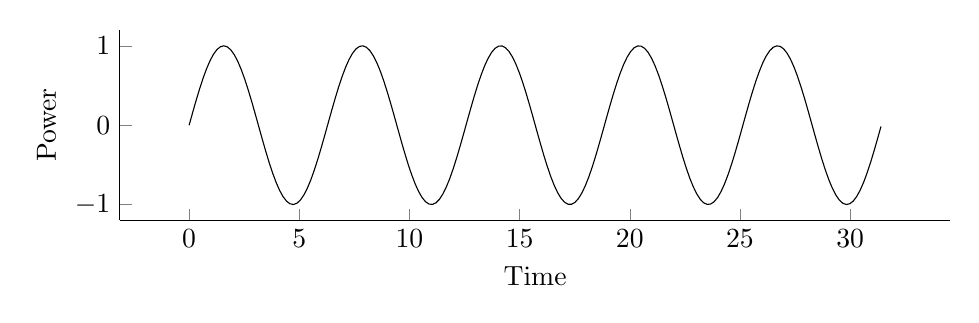
\begin{tikzpicture}
	\begin{axis}[
		axis lines*=left,
		width=\textwidth,
		height=4cm,
		ylabel=Power,
		xlabel=Time
		]
		\addplot [mark=none, black, domain=0:31.4, samples=200] {sin(deg(x))};
	\end{axis}
\end{tikzpicture}
\caption{An arbitrary sine wave in a time domain \emph{oscillogram} representation}\label{fig:sineTime}
\end{figure}

Time domain representations apply well to acoustic signals, where we can observe the progression of acoustic power over time to represent and analyze sounds.
In the simplest of cases, we can observe a single sine wave like the one in the oscillogram in \figref{fig:sineTime}. Here, a time domain representation is very informative with respect to the signal it depicts. The power, the (fundamental) frequency and the duration of the signal can all be readily deduced from this representation.
However, most natural sounds involve a much more complex distribution of acoustic power over different frequencies at different durations, many of them overlapping in time.
A time domain representation of complex natural sounds can effectively represent the overall impact of the many subcomponents on the amount of acoustic power at different points in time. It is, however, not very well suited to being informative with respect to any of the subcomponents of complex sound. Their individual frequencies, power and durations are all bundled together when we measure acoustic power over time.

We can decompose the complex signal into its subcomponents, provided that the subcomponents can be described as periodic signals, just like the simplest non-decomposable sine wave that characterizes acoustic signals. Doing that requires a switch from the time domain to the \emph{frequency domain}: rather than looking at the distribution of acoustic power over time, we can look at the distribution of acoustic power over different frequencies. A frequency domain representation allows us to observe the many subcomponents in terms of their frequency and power at given points in time.

Switching from time domain to frequency domain is possible with the \emph{Fourier transform}, a mathematical transform named after the French mathematician Jean-Baptiste-Joseph Fourier, who introduced it in \citet{fourier1822theoriesk}.
The Fourier transform decomposes a time series into a sum of finite series of sine or cosine functions.
Note that in many contexts of acoustic analysis, the procedure is referred to as \emph{fast Fourier transform} (FFT), which is the name given to a wide range of algorithms that perform quick calculations of the Fourier transform (see overview in \citealt{brigham1988fastsk}).

The time and frequency domains are two complementary, and, to some extent, redundant mathematical representations of the same physical reality.
By representing time as a scale of different potential rates, we can shift the representation of events in time into a representation of the co-activation of different rates in the frequency domain.
%It is perhaps useful to imagine the frequency domain as an interpretation of the time domain, whereby time is converted to one of its main effects -- the time-related impression of \emph{speed} (or \emph{rate}).
%Crucially, note that both domains are available for representation of physical events, regardless of timescales.

\subsection{Time and place theories in models of pitch perception}\label{sec:dualismPitch}

Models of pitch perception attempt to explain how the auditory system resolves the harmonic structure of complex signals into the sensation of pitch.
Two types of theories have traditionally dominated this field.
\emph{Place} theories of pitch are based on the idea that different frequencies in the signal can excite different places along the basilar membrane. \emph{Time} (or \emph{temporal}) theories of pitch are based on the idea that neural firing rates exhibit sensitivity in time to periodic events, allowing them to \emph{phase-lock} to the rate of periodicity in time.

Place theories of pitch often date back to \citet{ohm1843annalensk} and \citet{helmholtz1863lehresk}, and they are in line with the notion of the frequency domain (\citealt{ohm1843annalensk} in fact assumed that a Fourier analysis took place in the auditory system). Time theories of pitch often date back to \citet{seebeck1841annalensk, wever1930nature} and \citet{schouten1938perception}, and they are likewise in line with 
the notion of the time domain.
%time theories of pitch.
\citet{de2005pitch} traced back the early roots of these two pitch theories to ancient Greece, linking writings from Pythagoras (6th century BCE) and Aristoxenos (4th century BCE) with place theories of pitch, and linking the writings of Greek mathematician Nicomachus (2nd century CE) with time theories of pitch.

Place and time theories are sometimes presented as two dueling narratives, highlighting historical differences between \citet{seebeck1841annalensk} and \citet{ohm1843annalensk}, and later between \citet{helmholtz1863lehresk} and \citet{schouten1938perception} and many others. However, of consequence to this work is the more currently common appreciation that these two theories of pitch are, in fact, complementary and even desirably redundant to various extents (see \citealt{house1990tonal, de2005pitch, houtsma1995pitch, oxenham2013revisiting}).

\begin{sloppypar}
\citet{warren1981perception} mention the findings that frequency selectivity along the basilar membrane, which is essential for place-related pitch resolution, is roughly limited to 50--16k Hz \citep{bekesy1960experiments}, while phase-locking of the auditory nerve fibers' firing rate, which is essential for time-related pitch resolution, has a typical upper limit of about 5k Hz (\citealt{rose1967phase}; see a more recent review on this topic in \citealt{verschooten2019upper}).
\citet{warren1981perception} then make the point that the range in which both place and time models overlap, around 50--5k Hz is exactly the range for optimal perception of musical pitch.
\end{sloppypar}

\section{The spectral and temporal regimes of auditory perception}\label{sec:spectemp}

Auditory perception according to PRiORS is dramatically affected by two different responses to repetitions at two distinct timescales that constitute two perceptual regimes: the \emph{temporal regime} and the \emph{spectral regime}. The temporal regime designates the timescale at which humans can perceive successive acoustic events as isolated events in time, while exhibiting a relatively good ability to predict the upcoming event with a given steady rate, or perceive and estimate durations, in the related terminology of \citet{fraisse1984perception}. These upper and lower limits of perception were described in \citet[321]{macdougall1903structure} as conditions for \enquote{the impression of rhythm}, and, indeed, the timescale of the temporal regime defines the range at which musical rhythmic patterns tend to occur and auditory sensitivity to changes in rate allows us to reliably detect temporal patterns (e.g.~\citealt{fraisse1984perception, farbood2013temporal, repp2005sensorimotor}). In other words, the temporal regime covers our ability to perceive the difference between \emph{fast} and \emph{slow}.

The spectral regime, in contrast, operates at a faster timescale, where a sequence of acoustic events repeats too fast to be perceived as isolated events (see, e.g, \citealt{miller1948perception, broadbent1959auditory, efron1973conversation, hirsh1959auditory}). At these fast rates, rather than perceiving temporal intervals as occurring at non-overlapping moments in time, cognition switches to perceiving them as spectral intervals that occur at the same time, giving rise to the perception of a complex harmonic tone, whereby the harmonic partials reflect the rate of repetition in the spectral dimension (\citealt{flanagan1960pitch, stockhausen1959how, warren1982auditory}). Within the spectral regime, changes in rate of repetition of periodic signals are perceived as changes in pitch.
In other words, the spectral regime covers our ability to perceive the difference between \emph{high} and \emph{low} (pitch).\footnote{The notion of repetition is not limited to rate-based distinctions, but this work requires only this type of distinction to cover prosodic phenomena. To cover the acoustic qualities of segmental phenomena in speech we can analyze the lack of regular repetition at the spectral regime in at least two meaningful ways: (i) transient bursts are characteristic of speech sounds like \emph{stops} that exhibit a non-repeating signal (or more accurately, a critically damped signal); (ii) continuous yet irregular (asynchronous) repetitions within the timescale of the spectral regime are characteristic of \emph{aperiodic} noise that results from articulatory friction (e.g.~\emph{fricatives}).}

In principle, the temporal regime is congruent with the notion of \emph{time domain} and the spectral regime is congruent with the notion of \emph{frequency domain} (see \sectref{sec:dualismDomains}).
Likewise, the two regimes correspond to the two independent anatomical and neurological processes for pitch resolution that are also based on time and frequency representations (see \sectref{sec:dualismPitch}).
However, while the time and frequency domains can independently describe the same event in mathematical terms, and while place and time theories of pitch perception may be, to a large extent, complementary and redundant, the perceptual regimes in PRiORS operate at two slightly overlapping yet mostly distinct and mutually exclusive timescales.
Each perceptual regime responds to repetitions within its timescale such that a single quantitative modulation of the rate of repetition gives rise to qualitative differences in the sensation of rhythm (temporal regime), or, alternatively, the sensation of pitch (spectral regime).
In other words, the temporal and spectral regimes suggest a perceptual qualia perspective, whereby the two regimes are mutually exclusive.

This last point is reminiscent of Pattee's quote from \citet[21]{pattee2012lawssk}, which was given in \sectref{sec:compofmind}, and is partially repeated here:
\enquote{It appears that our artificial instruments have extended our senses beyond what our classical brains can model without cognitive dissonance.}
In that sense, the time and frequency domains in physics are revealed by our instruments as two overlapping representations, but in our mind, the temporal and spectral regimes are represented as two distinct and separate sensations.
To be clear, auditory perception can handle the two regimes at the same time, i.e.~process information with both rhythmic and periodic effects. The mutual exclusivity is in response to isolated events within their relevant timescale.

When evaluating PRiORS, it is useful to acknowledge how the auditory system is uniquely adapted to capturing reoccurrence in terms of repetition. \citet{chowning2001perceptual} suggests that the auditory system is far more sensitive than the visual system to differences in reoccurring structures. He reflects this ability in the visual system in terms of the capacity to detect minute differences in the spacing between otherwise identical objects (think of a typical \emph{spot the difference} puzzle as an example), essentially equating quasi-periodicity with quasi-symmetry.
\citet[267]{chowning2001perceptual} claims that the auditory system, unlike the visual system, \enquote{can readily detect a fraction of a percent of deviation from periodicity}.
This great sensitivity to repetition is linked in PRiORS to perceptual and cognitive aspects of an auditory system that is specialized in processing rhythm and pitch
as the two modes of auditory temporal integration.

\section{Visual FFT-based simulations}\label{sec:blitit}

It is useful to illustrate the distinction between perceptual regimes with a \emph{Band-Limited Impulse Train} (BLIT) synthesis that produces a train of transient acoustic bursts at adjustable rates.
Each burst is a single \emph{impulse}, which is the shortest electric burst a given system can produce, with equal power across the frequency scale (a perfect impulse has acoustic power over an infinite frequency range, but the impulses in a BLIT, as the name suggests, are band-limited to human hearing ranges, between approx. 20--20k Hz).\footnote{One major advantage of the BLIT synthesis concerns the minimal duration of impulses that allows the simulation to reduce confounding factors regarding burst duration. Longer bursts are expected to appear as more continuous at slower rates than comparable impulses because they fill a longer portion of the intervals between onsets of recurring events (i.e.~they have a longer \emph{tail}).}
The BLIT signal can be effectively visualized with standard FFT-based tools that convert signals between time domain and frequency domain representations (see \sectref{sec:dualism})

\tabref{tab:priorsTimeScales} presents a rough sketch of the relevant timescales of the two perceptual regimes. Within each regime the effects of repetition are named differently in order to maintain a distinction that attempts to be in-line with most common uses of these terms: it is \emph{Rhythm} when occurring within the timescale of the temporal regime vs.~\emph{Periodicity} when occurring within the timescale of the spectral regime. \tabref{tab:priorsTimeScales} also shows that these repetition-induced effects have boundaries. Repetitions within the temporal regime may be too slow to be perceived as rhythmic (\emph{infra-rhythmic} perception below 30 BPM; see \citealt{fraisse1984perception, farbood2013temporal}, and see overview of tapping literature in \citealt{repp2005sensorimotor}). Likewise, repetitions within the spectral regime may be too fast to be perceived as periodic (\emph{ultra-periodic} perception above 5k Hz, given that our auditory system can typically perceive frequencies up to 20k Hz, but our ability to sense discernible pitches does not typically exceed 5k Hz; see \citealt{ward1954subjective, attneave1971pitch}).%\footnote{To understand what it means that above 5k Hz we hear frequencies that do not support pitch perception it is useful to consider a comparison between a \emph{pure tone} (sine wave) at a given frequency and a \emph{white noise} signal that was band-pass filtered to very narrowly target the same frequency of the sine wave. The claim is that above 5k Hz the periodic sine wave and the aperiodic band-pass filtered noise will not sound very different from each other because our auditory system cannot detect the periodic structures at these fast rates .}


\begin{table}
\caption{\label{tab:priorsTimeScales}Perceptual regimes with corresponding effects and timescales (rough sketch). \textit{Note.} Hz = Hertz (repetitions per second); BPM = Beat Per Minute; ms = millisecond (duration of repeating intervals).}
\begin{tabular}{lcccc}
\lsptoprule
& & \multicolumn{3}{c}{{Timescales}}\\\cmidrule(lr){3-5}
Perceptual regimes & Effects & Hz & BPM & ms \\\midrule
Temporal & \multicolumn{1}{c}{\color{gray}Infra-rhythmic} & \multicolumn{1}{c}{\color{gray}0--0.5} & \multicolumn{1}{c}{\color{gray}0--30} & \multicolumn{1}{c}{\color{gray}∞--2k} \\
& \multicolumn{1}{c}{Rhythm} & \multicolumn{1}{c}{0.5--20} & \multicolumn{1}{c}{30--1200} & \multicolumn{1}{c}{2k--50} \\\midrule
Spectral & \multicolumn{1}{c}{Periodicity} & \multicolumn{1}{c}{20--5k} & \multicolumn{1}{c}{1200--300k} & \multicolumn{1}{c}{50--0.2} \\
& \multicolumn{1}{c}{\color{gray}Ultra-periodic} & \multicolumn{1}{c}{\color{gray}5k--20k} & \multicolumn{1}{c}{\color{gray}300k--1200k} & \multicolumn{1}{c}{\color{gray}0.2--0.05} \\
\lspbottomrule
\end{tabular}
\end{table}

Four examples are provided in \figref{fig:priors-blit}, each one with three corresponding visual panels. The bottom white panel presents a 1-second long waveform (\emph{oscillogram}) which shows the unipolar transient bursts produced by the BLIT synthesis in the time domain, going from left to right. The number of visible bursts within this 1-second interval corresponds to the rate of the BLIT in Hz. The two upper dark panels show FFT-based analyses exhibiting the dispersion of acoustic power across the audible frequency range in the frequency domain. The middle panel, often called a \emph{spectrograph}, exhibits a 2-dimensional representation of frequency (x-axis) and power (y-axis), while the top panel, which is typically called a \emph{spectrogram}, exhibits a 3-dimensional representation of frequency (x-axis), power (color) and time (y-axis). The frequency x-axes of the spectrograph and the spectrogram are perfectly aligned to facilitate the interpretation of the spectrograph in the middle as a \enquote{slice}, or a \enquote{still image} of the temporal representation in the spectrogram above it.



\begin{figure}
\includegraphics[width=1\linewidth]{extrenal_figures/blitCombScaled.png} 
\caption{Illustration of perceptual regimes with visual analyses of acoustic impulse trains (BLIT) at different rates and different domains (see text for details).}\label{fig:priors-blit}
\end{figure}

\figref{fig:priors-blit}(a) (top left) shows a clear rhythmic effect at 4\,Hz, indicated by four bursts in the bottom oscillogram panel. A single burst appears with equal power along the (band-limited) frequency range in the spectrograph, indicated by the fairly straight horizontal green line across the middle panel.
Note that the still image shown here captured a moment in time in which the power graph of the spectrograph was high. With rhythmic bursts, like the 4\,Hz BLIT in \figref{fig:priors-blit}(a), this graph goes visibly up and down over time. Above it, a succession of 10 impulses over a short period of time (about 2.5 seconds) is visible as isolated bursts, indicated by the horizontal lines going from bottom to top in the corresponding upper spectrogram panel.

In sharp contrast, \figref{fig:priors-blit}(d) (bottom right) clearly shows tonal behavior at 120\,Hz. There are, indeed, 120 bursts in the time-domain display of the bottom oscillogram panel, but the isolated bursts are no longer visible in the top spectrogram panel, i.e. there are no horizontal lines going from bottom to top across the upper panel (note that with the 2.5 second-long window of the spectrogram, 120 bursts per second should have resulted in 300 horizontal lines by comparison to \figref{fig:priors-blit}(a)).
The sensation of isolated discrete bursts transitions into a sensation of continuous sound in perception at these higher rates of repetition. This can be thought of as a smearing effect that occurs above a certain threshold. This perceptual effect is neatly reflected by the two FFT-based representations in \figref{fig:priors-blit}(d), which display a signal with the properties of a continuous sound that has a complex harmonic structure. The middle spectrograph panel shows a series of \enquote{bumps} along the green curve, from left to right, corresponding to a series of continuous energy \enquote{poles} in the vertical representations of the upper spectrogram panel. This is a harmonic series in which the rate of repetition of the BLIT synthesis is mapped onto the fundamental frequency (F0) of the continuous sound, which is also manifested in the distance between partials in the harmonic series.\footnote{The polarity of the impulses can also play a role with pitch perception at higher rates within the spectral regime, as demonstrated in \citet{flanagan1960pitch}. For this reason, I used only unipolar impulses for which the relationship between impulse rate and frequency rate is kept stable.} Specifically, the two FFT-based representations in \figref{fig:priors-blit}(d) show the harmonic partials in terms of continuous acoustic power at the frequencies 120\,Hz, 240\,Hz, 360\,Hz, 480\,Hz, etc.
This demonstrates that at this faster timescale of the spectral regime, the sensation of repetition feeds perceptual effects of continuity and pitch, rather than of discreteness and rhythm.

The switch between regimes does not occur at once. Between the temporal and the spectral regime, we can spot a transitional range in which effects of both rhythm and periodicity are present, but neither is strong enough to completely take over. This results in a less definitive effective sensation.
Figures~\ref{fig:priors-blit}(b--c) demonstrate this transitional range between the two distinct regimes that are illustrated by \figref{fig:priors-blit}(a) (for the temporal regime) and \figref{fig:priors-blit}(d) (for the spectral regime), as detailed above.

\figref{fig:priors-blit}(b) (top right) is especially well-suited for illustrating the indeterminacy of the transitional range. At a BLIT rate of 24\,Hz, the impulses seem to be too fast to support a rhythmic perception of discrete bursts, and, at the same time, too slow to support the perception of a continuous harmonic (pitch-bearing) sound. The upper spectrogram panel of \figref{fig:priors-blit}(b) shows a combination of both horizontal lines that reflect isolated events in time, going from bottom to top, as well as vertical lines that reflect the emerging harmonic structure of a continuous complex tone (visible also as corresponding energy fluctuations in the middle spectrograph panel).

\begin{table}
\caption{\label{tab:transitionalTimeScales}Rough sketch of perceptual regimes with corresponding effects and timescales (transitions included). \textit{Note.} Hz = Hertz (repetitions per second); BPM = Beat Per Minute; ms = millisecond (duration of repeating intervals).}
\begin{tabular}{lcccc}
\lsptoprule
& & \multicolumn{3}{c}{Timescales}\\\cmidrule(lr){3-5}
Perceptual regimes & Effects &  Hz & BPM & ms \\\midrule

Temporal & \multicolumn{1}{c}{\color{gray}Infra-rhythmic} & \multicolumn{1}{c}{\color{gray}0--0.5} & \multicolumn{1}{c}{\color{gray}0--30} & \multicolumn{1}{c}{\color{gray}∞--2k} \\
   & \multicolumn{1}{c}{Rhythm} & \multicolumn{1}{c}{0.5--12} & \multicolumn{1}{c}{30--720} & \multicolumn{1}{c}{2k--83.3} \\
   & \multicolumn{1}{c}{\color{gray}Ultra-rhythmic} & \multicolumn{1}{c}{\color{gray}12--20} & \multicolumn{1}{c}{\color{gray}720--1200} & \multicolumn{1}{c}{\color{gray}83.3--50} \\\midrule
Spectral & \multicolumn{1}{c}{\color{gray}Infra-periodic} & \multicolumn{1}{c}{\color{gray}20--50} & \multicolumn{1}{c}{\color{gray}1200--3k} & \multicolumn{1}{c}{\color{gray}50--20} \\
   & \multicolumn{1}{c}{Periodicity} & \multicolumn{1}{c}{50--5k} & \multicolumn{1}{c}{3k--300k} & \multicolumn{1}{c}{20--0.2} \\
   & \multicolumn{1}{c}{\color{gray}Ultra-periodic} & \multicolumn{1}{c}{\color{gray}5k--20k} & \multicolumn{1}{c}{\color{gray}300k--1200k} & \multicolumn{1}{c}{\color{gray}0.2--0.05} \\
\lspbottomrule
\end{tabular}
\end{table}

To consider the transitional phases between the two regimes, \tabref{tab:transitionalTimeScales} pres\-ents a slightly more elaborate sketch than \tabref{tab:priorsTimeScales}, with transitional phases at 12--50\,Hz. Essentially, this emphasizes the fact that the main effects -- rhythm sensation in the temporal regime and periodic sensation in the spectral regime -- are optimally achieved closer to the center of each perceptual regime.

Note that the visual effects of the FFT-based representations in \figref{fig:priors-blit} are calibrated to reflect human perception.\footnote{Here I use a commercial metering application, SpectraFoo by Metric Halo (version 4.2.3), with the default Analyzer depth setting of 4,096 points (10\,Hz). The BLIT synthesis and the oscillogram were produced with the sound design software Plogue Bidule (version 0.9766).} The shift from temporal to spectral regimes does not represent a change in any physical quality. Rather, it represents a perceptual threshold of a given system.
A different system that responds to higher rates of periodicities, such as, for example, models simulating the auditory system of barn owls (see \citealt{koppl1997phasesk}), will most probably require higher frequencies to adequately represent the shift from the temporal to the spectral regime. Importantly, higher frequencies will require higher resolutions before the temporal representation becomes too fast and eventually \enquote{smears} into the spectral one.

\section{A note about previous works}\label{a-note-about-previous-works-warren-and-rosen}

The ideas in PRiORS are not entirely new. For one, they are not based on any new data, but on established findings in the literature from the fields of acoustics, auditory perception, neuroscience and linguistics. More specifically, previous proposals were presented in the past for frameworks of perception that are, much like PRiORS, based on delineating the unique contribution of different timescales to auditory perception.
I will summarize two of these in the following.

\begin{sloppypar}
Richard Warren, who studied temporal integration in auditory perception quite extensively, sketched a model with different perceptual effects at different timescales in \citet{warren1981perception} and \citet[80--85]{warren1982auditory}. \citet{warren1981perception} determined that 50--5k Hz is the optimal timescale for pitch perception (\enquote{melodic pure pitch}), given that in this range, both place-based and time-based resolutions of pitch are available.
At faster rates of 5k--16k Hz, where only place-based pitch resolution may be available, an \enquote{amelodic pure pitch} perception takes over.
At slower rates, between 20--50\,Hz, with only time-based pitch resolution available, the \enquote{pure pitch} sensation changes to \enquote{noisy pitch}. Further down, below 20\,Hz, repetitions are considered by \citet{warren1981perception} as \emph{infrapitch}, as they are too slow to induce a sensation of pitch.
\citet{warren1981perception} follow \citet{guttman1963lower} in determining 0.5\,Hz as a rough lower floor for perceptual integration of acoustic events. This 0.5\,Hz floor of about 2 second-long intervals is commonly mentioned as the lower threshold of the human ability to keep isochronous rhythm or temporally integrate events (see \citealt{fraisse1984perception, farbood2013temporal, repp2005sensorimotor}).
\end{sloppypar}

Approaching auditory perception of speech from a more linguistic point of view, \citet{rosen1992temporal} presented a framework for describing temporal information in speech, which can also be considered as a precursor of the PRiORS framework.
In his framework, \citet{rosen1992temporal} divides perception into three \enquote{temporal features} at distinct timescales: \emph{envelope} (2--50\,Hz), \emph{periodicity} (50--500\,Hz) and \emph{fine-structure} (600--1k Hz). \emph{Envelope} covers mainly \enquote{tempo, rhythm} and \enquote{syllabicity}, while \emph{periodicity} covers mainly \enquote{stress}, \enquote{intonation} and \enquote{voicing} (see \cite[76]{rosen1992temporal}, in which other segmental qualities are also covered).

\section{Advantages of PRiORS}\label{advantages-of-priors}

The PRiORS framework is useful for understanding various phenomena in auditory cognition and in phonological systems. It can be useful for models of speech perception that consider the contribution of auditory perception and cognition to language systems, as was detailed in \chapref{sec:lingMod}, and especially \sectref{sec:missinglinks}.
The following subsections address two major points that PRiORS can greatly help to elucidate. In Section~\ref{sec:universal} I discuss how PRiORS can dispel a lot of the mystery surrounding the phonological notion of the \emph{syllable}, and in Section~\ref{sec:quasi} I discuss PRiORS' potential for uncovering the different functions that music and speech utilize when they wield the effect of \emph{rhythm} from the timescale of the temporal regime.

\subsection{Universal aspects of syllabic structure}\label{sec:universal}

\begin{figure}
\includegraphics[width=1\linewidth]{extrenal_figures/SyllableSinesExtended} 
\caption{Schematic illustration of the relationship between perceptual regimes and syllabic units, using the three canonical syllables of the English word \emph{syllable} (demonstrated with one possible underlying annotation). Segmental makeup, i.e.~\emph{sonority}, is related to the spectral regime with high-frequency (\emph{periodic}) oscillations within syllables, while syllabic speech rate is related to the temporal regime with low-frequency (\emph{rhythmic}) oscillations between syllables. The ratio between the low-frequency and high-frequency oscillations in this illustration is arbitrarily set to be 1:20. This is a realistic ratio for syllables such that if syllables are taken to have a typical duration of 200\,ms (5\,Hz), the high-frequency oscillation within it would reflect a typical F0 for adult males at 100\,Hz. For simplicity, this generalized illustration shows a single rate at each timescale with isochronous repetitions (see Section~\ref{sec:quasi} on the more complex picture regarding isochrony in speech).%rather than quasi-repetitive ones (see Section~\ref{sec:quasi}).
}\label{fig:syll-sines}
\end{figure}

Syllables are, first and foremost, abstract units of phonological systems and they do not easily lend themselves to consistent and straightforward phonetic explanations in terms of perception and/or articulation.
The PRiORS framework can do a lot of heavy lifting in this regard, by providing the baseline conditions that can explain the evolutionary trajectory of syllables. According to this analysis, syllables were shaped by selection to optimally take advantage of the two perceptual regimes:
carrying pitch in the spectral regime and giving rise to speech rate relations in the temporal regime
(see \citealt{rasanen2018pre} for a similar type of analysis).
In other words, syllables have an internal segmental makeup that is optimized to carry pitch in order to exploit the distinction between low vs.~high periodicity in the spectral regime, and, at the same time, they appear in sizes that allow the distance between them to give rise to speech rate effects in order to exploit the distinction between slow vs.~fast rates in the temporal regime.
\figref{fig:syll-sines} illustrates this state of affairs with a highly generalized schematic sketch of the slower rhythmic cycle between syllables and faster periodic cycles within syllables.

PRiORS can therefore explain the universality of the typical syllable size and the universality of the preferred segmental makeup in the syllabic nucleus, which is commonly measured in linguistic terms of \emph{sonority}.
In line with PRiORS, this work claims that sonority should be understood as a measure of pitch intelligibility, acting as a defining feature of syllabic nuclei.
Syllables therefore need to be long enough to allow a minimum amount of periods to be effectively perceived.
For example, a very low F0 of 50\,Hz, which repeats every 20\,ms, requires a minimum of 3 periods (60\,ms) to be perceived, while higher F0 values (which characterize most speech) repeat faster and require even shorter minimum intervals (\citealt{fyk1987duration, josephs1967thephysics}). It is of interest to note that the average duration of syllables is about 200\,ms (5\,Hz, 300\,BPM), which is enough for adequate perception of pitch, as well as being at the center of the temporal regime, where it is optimally situated to achieve speech rate effects from the distance between syllables.

\subsection{Speech is quasi-repetitive}\label{sec:quasi}

The notion of repetition implies identical intervals between occurrences over time, i.e.~repetition is taken to be \emph{isochronous} unless otherwise stated. It has long been noted that pitch-inducing speech sounds are in fact not fully-isochronous, but, rather, \emph{quasi-periodic}, as the pitch and its underlying periods are often unstable at some level.
The notion of quasi-repetitiveness is mostly used to refer to an inherent \emph{jitter} in the regularity of repeating patterns that prevent perfect isochrony. This level of jitter (or noise) in the voice is assumed to be perceptually negligible.
However, on top of that there is another -- much larger -- source of apparent instability in repetitive structures in speech.
Speech is dynamically changing all the time, in magnitudes that far exceed the levels of inherent jitter, in order to achieve perceptible goals and to effectively exploit the sensations of rhythm and pitch.

Consider for example the periods during a rising pitch contour, in which every period is shorter than the previous one.
These degrees of change do not hinder the perception of coherent pitch contours, demonstrating our specialized ability to perceive dynamically-changing pitch.
As long as these communicatively relevant pitch differences occur within the timescale of the spectral regime
(and follow basic Gestalt principles)
they invoke a reliable effect in perception.
It is exactly these dynamic changes in the rate of repetition that prosody seems to exploit in speech.

A similar behavior can be observed for rhythm in speech. Speech rates do not typically appear as isochronous within the rhythm-inducing timescale of the temporal regime (see  \citealt{turk2013speechsk} and \citealt{nolan2014speechsk}). This is the temporal range which is exploited in speech for its perceptible effect on speech rate in terms of slow vs.~fast.
Crucially, there are no strong reasons to assume that the effect of rhythm in speech is exploited for isochrony, as it is not clear what purpose this would serve in speech.
However, in order to achieve various prosodic goals such as phrasal demarcation, turn-taking management and prominence marking (among many others), asynchronous temporal relations are exploited within the scope of speech rate sensations. In other words, speech is also \emph{quasi-rhythmic} and dynamically changing at the timescale of the rhythm-inducing effects of the temporal regime in order to be effective for prosody.

Confusingly, speech makes a very different usage of the temporal regime when compared to music, which, more often than not seems to favor isochronous rhythmic patterns over meandering ones within the rhythm-inducing timescale.
Musical experiences tend towards isochronous rhythms, perhaps because of the powerful ability of the perception of isochrony to create a shared clock that can be synced across separate systems and human agents, whereby different people can couple sensorimotor oscillations between one another and experience \emph{entrainment} (see, e.g., \citealt{cummins2009rhythm, cummins2015rhythm, benichov2016finding, haegens2018rhythmic, kotz2018evolution, rouse2016beat, tal2017neural}).

In contrast to a classic case of entrainment to external clocks, languages seem to use the effects of rhythm in the temporal regime for a different set of goals that do not seem to require isochrony and should not be considered to reflect classic entrainment (see, e.g., \citealt{cummins2012oscillators} and \citealt{meyer2019synchronous}).
%(see also \cite[1]{cummins2012oscillators}, on speech being insufficiently isochronous to support entrainment). 
The rhythm-inducing timescale is mostly used in speech to effectively exploit the distinction between slow and fast speech rates as useful cues in a system of speech prosody.
To that end, 
(quasi-)isochrony
%the most (quasi-)isochronus element 
in speech perception should be considered as internal (\textit{endogenous} neural activity) rather than external (\textit{exogenous} neural activity), to allow the hearer to infer the dynamic (and largely unpredictable) changes in the speech rate of their interlocutors.

%In other words, isochrony is not to be found 
%%(i.e. not 
%in the speech signal itself but in the mind of the hearer. This is needed in order to allow interlocutors to effectively perceive the (largely unpredictable) rate of external speech of other interlocutors. The speech rate 

%as they effectively employ it in their prosody.
Thus, a striking feature of the effects of %repetition 
auditory temporal integration
in language is that they make use of the two perceptual regimes by keeping repetitive elements in a constant state of flux within their effective timescales. To be communicatively useful in prosody, pitch in speech is mostly quasi-periodic and highly dynamic within a privileged range of pitch perception. Likewise,
%and 
speech rate is mostly quasi-rhythmic and highly dynamic within a privileged range of rhythm perception.
%This is the case both in terms of the perceptually negligible jitter and the perceptually informative dynamic changes in rate.
%In other words, both rhythm and pitch in speech prosody are a moving target that can be adequately represented as a smooth continuous trajectory (see Section~\ref{sec:speechRate} for preliminary implementations of this idea).

\section{Neural oscillations in perception and cognition}\label{sec:neuro}

\begin{table}
\caption{\label{tab:oscillationsTimeScales}Generic neural oscillations (roughly defined) across the temporal regime}
\begin{tabular}{lccc}
\lsptoprule
Perceptual regimes & Effects & Neural Oscillations & Timescales (Hz)  \\
\midrule
Temporal & Rhythm &  \emph{delta} & 0.5--4\phantom{2} \\
&   &                \emph{theta} & \phantom{0.}4--8\phantom{2} \\
&   &                \emph{alpha} & \phantom{0.}8--12 \\
\lspbottomrule
\end{tabular}
\end{table}

The PRiORS timescales also fit very well with the characterization of speech processing via neural oscillations of brain activity at different wave lengths (see overviews in \citealt{buzsaki2006rhythms, myers2019pushing, poeppel2020speech}). As \tabref{tab:oscillationsTimeScales} demonstrates, three distinct neural activity patterns are commonly observed within the rhythmic portion of the temporal regime, comprising a set of low frequency oscillations. Interestingly, the mid-range among the three, the \emph{theta} frequency band at 4--8\,Hz, has been often studied in conjunction with syllables, as it covers the range of durations (125--250\,ms) that, indeed, characterizes the vast majority of syllables cross-linguistically (\citealt{ding2014robust, ding2017temporal, gross2013speech, keitel2017auditory, luo2010auditory, poeppel2020speech}).

The link between the theta frequency and syllables is consistent with the PRiORS framework, whereby syllables and the temporal domains of cognition are assumed to have co-evolved to exploit the rhythmic effects of the temporal regime, therefore tending towards the center of this particular perceptual-cognitive sensation.

Note that the timescales of speech units do not necessarily fall into the classic division of generic wave lengths. Syllables can be quite diverse and they can be found at rates ranging from 2\,Hz, with long 500\,ms intervals (e.g.~\citealt{chandrasekaran2009natural}), to 20\,Hz, with short 50\,ms intervals (e.g.~\citealt{greenberg2003temporal}).
Likewise, various speech phenomena have been associated with the ranges of delta and theta waves (1--8\,Hz), i.e.~at intervals ranging from a little over 100\,ms up to one second (e.g.~\citealt{ghitza2017acoustic, ghitza2013theta, cummins2012oscillators, goswami2013speech, inbar2020sequencessk, meyer2017linguistic}).

\citet{keitel2018perceptually} focus on timescales directly extracted from statistical regularities in their speech material, rather than focusing on generic timescales like delta or theta bands. The timescales in their study reflected the rates of \emph{phrases} (0.6--1.3\,Hz), \emph{words} (1.8--3\,Hz), \emph{syllables} (2.8--4.8\,Hz), and \emph{phonemes} (8--12.4\,Hz) as they appeared in their corpus of carefully read speech (by a trained, male, native British actor). Indeed, after analyzing corresponding speech tracking signals from listeners using magnetoencephalography (MEG), they found neural activity strongly correlated to these timescales. PRiORS can shed light on such results, whereby, as with the generic waves, the timescale of syllables occupies a central portion of the rhythm-inducing range of the temporal regime (2.8--4.8\,Hz). Furthermore, all the different linguistic units are neatly spread across the rhythm-inducing range, defined here at 0.5--12\,Hz (see \tabref{tab:transitionalTimeScales}), allowing speakers to perceive quasi-rhythmic patterns of stressed and emphasized/accented syllables at the lower end of the rhythmic perception that \citet{keitel2018perceptually} link with \enquote{phrases} (0.6--1.3\,Hz) and \enquote{words} (1.8--3\,Hz), as well as perceiving quasi-rhythmic patterns of segment-size units that \citet{keitel2018perceptually} link with \enquote{phonemes} at the highest end of rhythmic perception (8--12.4\,Hz).

Note that the transitional range between regimes in PRiORS, defined here as roughly 12--50\,Hz (see \tabref{tab:transitionalTimeScales}), is expected to be of little usefulness for bottom-up processing of auditory material given that at this timescale the effects of rhythm and periodicity are somewhat indeterminate.
The neural oscillations that are commonly associated with this timescale are the \emph{beta} band at about 13--30\,Hz and the \emph{gamma} band at about 30--50\,Hz.
Interestingly, studies such as \citet{mai2016deltask} and \citet{keitel2018perceptually} find the beta and gamma rates of neural oscillation to be more closely related to top-down inferences involved in processing of syntax and semantics. This implies a functional division of labor when processing speech, whereby top-down inferences may \enquote{piggyback} on channels that are less useful for bottom-up processes.

%\subsection{Genetic evidence for PRiORS' impact on phonology}\label{genetic-evidence-for-priors-impact-on-phonology}

Recent work in \citet{tang2020dcdc2sk} is in line with the rationale of the PRiORS framework, linking phonological outcomes with the same perceptual primitives that the PRiORS framework assumes. \citet{tang2020dcdc2sk} investigate the relationship between the frequency of certain genes in human populations and phoneme inventories in their respective languages.
The genes they investigate are assumed to modify faithful spectral and temporal encoding in the auditory cortex. It appears that the distribution of these genes across human populations can quite reliably predict the size of stop and nasal consonant inventories that will be featured in their languages. The authors suggest that the differences in spectral and temporal precision that can explain these phonemic preferences, may be directly related to observed differences in genetic expressions.

\section{Shifting paradigms in linguistic theory with PRiORS}\label{sec:shiftPar}\largerpage

The most relevant areas of phonological theory that PRiORS can shed light on concern the notions of sonority (see Section~\ref{sec:shiftSonority}), as well as the notion of rhythm in speech. Rhythm is beyond the scope of the current study, but some pointers towards the potential contribution of PRiORS are given in Section~\ref{sec:shiftRhythm} below.

\subsection{A different rhythm}\label{sec:shiftRhythm}

The idea that the effect of rhythm in speech has the same function as rhythm in music has misled many attempts to characterize rhythm phenomena in speech.
The thorniest challenge that such endeavors have to face is the search for isochrony in conversational speech that is not chanted or sung.
A strict view of isochrony, which is sometimes referred to as \emph{coordinative} or \emph{periodic} rhythm, is very characteristic of what we typically consider to be rhythmic in musical terms -- the division of time into equal parts (and the further subdivisions of those equal parts into simple fractions: 1/2, 1/3, 1/4, 1/8, 1/16, etc.).

A well-known manifestation of this search for isochrony can be found in the typological classification of \emph{stress-timed} vs.~\emph{syllable-timed} languages (see \citealt{pike1945intonationsk, abercrombie1967elements, dauer1983stress, lehiste1990phonetic}), whereby isochrony is supposedly maintained between syllables in syllable-timed languages and between stressed syllables in stress-timed languages. According to this idealized view, languages that do not reduce unstressed syllables (e.g.~Spanish) maintain isochrony between all the syllables within a phrase, while languages like English, with secondary stress and reduction of unstressed syllables, maintain isochrony only between the stressed syllables within a phrase (such that reduced syllables do not participate in this timing scheme).
This view is idealized since a straightforward isochrony of this type, in which some level of spoken language adheres to an external clock, is not to be found on the surface acoustics of speech (e.g.~\citealt{arvaniti2009rhythm, turk2013speechsk}).

A slightly more nuanced concept of rhythm targets the relationship between speech items,
rather than the alignment of speech items to real time.
It is sometimes referred to as \emph{contrastive} or \emph{phonological} rhythm as it addresses our tendency to perceive a strong/weak distinction between repeating items in a sequence. This conception of rhythm does not assume strict isochrony that adheres to an external clock. Instead, it uses local timing relations to reflect prominence and grouping in the speech signal (e.g.~\citealt{arvaniti2009rhythm}).

Various acoustic metrics were developed in order to measure global rhythmic distinctions, with the aim of characterizing different languages. Among them are measurements of the relative abundance or regularity of durations of selected units such as vowels and consonants, e.g.~\%V, ∆V, ∆C \citep{ramus1999correlates}, \emph{VarcoV}, \emph{VarcoC} \citep{dellwo2006rhythmsk} and variants of the \emph{Pairwise Variability Index} (PVI) (e.g.~\citealt{grabe2002durational}).
These metrics manage to avoid the requirement for strict isochrony and they succeed in characterizing different languages, but this seems to be true only to some extent, with small effect sizes (the variability within languages can be very high due to various factors like speech style and methodological decisions in the measurement itself) and in manners that are inconsistent with classic rhythm typologies
(see \citealt{arvaniti2012usefulness}). \citet{lowit2014quantification} concluded that none of these metrics are useful in clinical settings, based on systematic comparisons between speakers with dysarthria and matched healthy participants.

\citet{nolan2014speechsk} provide an overview of these problems. They suggest that language is perhaps \emph{antirhythmic} such that isochronous patterns are not to be found in the surface acoustics, but they might be metaphorically projected in perception. This description is indicative of the fact that even the concept of \emph{contrastive} rhythm is essentially based on comparison to an isochronous baseline, as if isochrony is an underlying goal of speech rhythm in and of itself.

PRiORS can help us make the next logical step by providing a slightly different framework for the understanding of rhythm, such that isochrony is no longer a key ingredient in its definition. Isochrony is one goal that can be achieved from rhythm effects in the temporal regime, and, indeed, this goal is exploited extensively in music.
Music seems to exploit rhythm effects to achieve isochrony in order to promote entrainment, while speech seems to exploit rhythm effects in order to control the temporal dimension of prosody and effectively use the distinct sensation of slow vs.~fast.
Speech -- unlike music -- is mostly meandering in its rhythmic patterns.
Expecting rhythm in speech to exhibit isochrony is akin to an expectation that every syllable would have a steady level pitch in order to count as periodic,
overlooking the major role
of perceived dynamic changes within each perceptual regime
(see Section~\ref{sec:quasi}).

Rhythm in speech should therefore be understood as a moving target that can be more adequately modeled in terms of a trajectory, much like the trajectory of the F0 at the faster timescale of the spectral regime.
Related ideas towards this goal can be found in the
pioneering work of \citet{pfitzinger2001phonetischesk}, which uses dynamic trajectories to describe local speech rate. A PRiORS-based analysis of rhythm in speech should therefore target the syllable-size fluctuations in the periodic energy curve, and model their temporal distances in terms of a dynamic smooth trajectory in order to capture local speech rate as the main effect of rhythm in speech (for preliminary attempts, see Section~\ref{sec:speechRate}).

\subsection{A new type of sonority}\label{sec:shiftSonority}

The human auditory system evolved to exhibit great sensitivity to (quasi-)pe\-ri\-od\-ic signals within the spectral regime, specializing in the perception of pitch. This is evident from the impact of pitch on our categorization of many musical sounds (e.g.~\citealt{bidelman2009neural}) as well as on tone and intonation in speech (e.g.~\citealt{krishnan2005encoding}).
This is also evident from anatomical and neurological activity, either in terms of \emph{place} representations in the cochlea (i.e.~in spectral terms) or in terms of \emph{timing} representations in the auditory nerve, characterized by \emph{phase-locking} to neural firing rates (see Section~\ref{sec:spectemp}).

The \emph{vocalic} or \emph{voiced} portions of speech can be described as a train of glottal pulses produced by vocal fold vibration, not unlike the idealized BLIT simulation in Section~\ref{sec:blitit}. This voiced component of the speech signal is the main carrier of pitch in speech and it is a striking fact about all languages that they prefer this auditory characteristic at the nucleus of their syllables (as well as the fact that all known languages exhibit a syllabic structure to begin with).

One aspect of this important dimension of linguistic sound systems is our ability to obtain good estimations of the \emph{fundamental frequency} (F0) of complex sounds, which we take as a reliable correlate of perceived pitch height. Indeed, phonologists and phoneticians have incorporated continuous measurements of F0 as a regular part of their toolbox, and they are well aware of the fact that F0 is more robust at syllabic nuclei, where the most sonorant elements usually sustain a sufficiently long and powerful (quasi-)periodic sound (see \citealt{barnes2011voicelesssk, barnes2014segmentalsk, roettger2019tune}).

Measurements of F0 therefore cover a qualitative aspect of perceived pitch: its height in terms of the rate of repetition of the fundamental frequency.
What is missing from this picture is the quantitative aspect of this auditory dimension, a description of acoustic power that targets only the pitch-inducing (vocalic/periodic) portions of the speech signal, unlike the commonplace practice to obtain the physical \emph{intensity} of the acoustic signal as a whole. A measurement of this kind, referred to as \emph{periodic energy}, has the promising ability to correlate with the notion of \emph{sonority} in a way that implies causation related to \emph{pitch intelligibility}, as it separates pitch-inducing components that favor syllabic nuclei from noise-inducing aperiodic components that favor syllabic margins.

Sonority in this sense is viewed as a measurement of the goodness of fit for syllabic nuclei, directly targeting pitch as an auditory dimension that our perceptual-cognitive systems are specialized for and that has evidently shaped the basic structure of all linguistic sound systems, given the universality of syllables with sonorous/pitch-bearing nuclei.

The perspective that PRiORS suggests helps in redirecting our focus away from the non-discriminative nature of general acoustic intensity and other acoustic measurements that do not suggest a clear and consistent association with perception and cognition. Instead, PRiORS directs us to search for acoustic measurements that exhibit robust links to pitch-inducing phenomena in the spectral regime in order to adequately characterize sonority.
As PRiORS helps elucidating, periodic sounds in the acoustic speech signal carry valuable pitch information, which, in turn, makes them privileged in terms of position within the syllable.

 \chapter{Sonority, pitch and the Nucleus Attraction Principle (NAP)}\label{sec:sonPitch}

\section{Sonority and pitch intelligibility: A causal link}\label{sec:pitchintelligibility}

The observation that sonority summarizes an essential quality that is related to vowels and their propensity to deliver a relatively steady harmonic structure, highlighting pitch and formant information, is by no means new. Previous proposals already defined sonority as either relating to vowels in some general way, more specifically relating it to voicing or glottal fold vibration, or to the clarity/strength of formants.\footnote{A partial list of some prominent examples includes \citet{sigurd1955rank, jakobson1956fundamentals, chomsky1968spesk, foley1972rule, ladefoged1971preliminaries, allen1973accentsk, fujimura1975syllable, Donegan1978onthenatural, ultan1978typological, price1980sonority, lindblom1983production, anderson1986suprasegmental, vennemann1988preferencesk, levitt1991syllable, pierrehumbert1992lenition, fujimura1997acoustic, stemberger1997handbook, boersma1998functional, zhang2001effects, howe2004harmonic, clements2009does, sharma2018significance}.} A few previous accounts went even further, by addressing the function of this evasive vowel-centric feature, suggesting that sonority may be related to periodic energy or pitch/tone (\citealt{heselwood1998unusual, ladefoged1997linguistic, lass1988phonology, nathan1989preliminaries, puppel1992sonority}). What all these proposals share, explicitly or implicitly, is a recurring insight about a strong link between the preferred type of segmental material in syllabic nuclei and a set of features that conspire to optimize pitch intelligibility, a property which characterizes vowels more than consonants.

Pitch is an indispensable communicative dimension of all linguistic sound systems (\citealt{bolinger1978intonation, cutler1997prosody, house1990tonal, roettger2019tune}), whether it is lexically determined as in linguistic \emph{tone},
or post-lexically employed to convey intonation, i.e. the linguistic \emph{tune} (see typological accounts of prosodic systems in \citealt{jun2005prosodicsk, jun2015prosodicsk}).
Tones are used to distinguish lexical items while tunes are used to demarcate units,
to modulate semantics (e.g.~information structure and sentence modality) and to
express a vast array of non-propositional meanings (e.g.~discourse-pragmatic intention, emotional state, socio-indexical identity, and attitudinal stance). The importance of pitch to human communication cannot be overstated.

Crucially, linguistic pitch events are known to target syllable-sized units as their \enquote{docking site}, regardless of the type of pitch event, whether they are lexical tones or post-lexical tunes.
These linguistic pitch events are commonly considered to associate with \emph{tone-bearing units} (see \citealt{leben1973suprasegmental}), that are either syllables or \emph{moras}.\footnote{Moras are used to represent quantitative differences between light and heavy syllables (\emph{weight sensitivity}, see Section~\ref{sec:attraction}), such that light syllables contain one mora while heavier syllables contain two (and sometimes even three) moras (see \citealt{hyman1984atheory, hayes1989compensatory, ito1989prosodic, mccarthy1990footsk, zec1995sonority, zec2003prosodic}).}
These associations between the text on the one hand and tone or tune on the other hand are widely assumed to be mediated by syllabic/moraic units.
For example, intonation pitch contours that highlight and modulate whole words and phrases essentially target privileged syllables -- \emph{heads} (stressed syllables) and \emph{edges} (syllables at initial and final positions of prosodic words and phrases) -- to achieve their communicative goal on textual material of various sizes.
This tone-bearing role of syllables and moras is the hallmark of many prominent theories regarding tone and intonation, following from Autosegmental and Autosegmental-Metrical Phonology (e.g.~\citealt{liberman1975intonationalsk, goldsmith1976autosegmental, ladd2008intonational, pierrehumbert1980phoneticssk}).

The functionally motivated conclusion that emerges with respect to sonority is therefore that syllables require a pitch-bearing nucleus and that sonority is a scalar measure of the ability to bear pitch. In other words, sonority is, most likely, a measure of \emph{pitch intelligibility}.
This hypothesis comes with an underlying assumption that was introduced by the PRiORS theoretical framework in \chapref{sec:priors},
whereby syllables are claimed to have followed an evolutionary trajectory that shaped them to optimally carry pitch in their nuclei (Section~\ref{sec:universal}). Sonority, according to this description, serves as the tool that governs the requirement for intelligible pitch as a fundamental characteristic in the design of the building blocks of prosody (see Section~\ref{sec:shiftSonority}).

It is important to note that this view of sonority is explicitly and exclusively based on perception, rather than articulation of speech. However, it does not exclude articulation-based description of syllables under the assumption that restrictions on syllabic structure must be derived from both the perception and the articulation of speech. A case in point is the \emph{Articulatory Phonology} framework
(see \sectref{sec:synthesis}),
with its valuable descriptions of temporal coordination and phase relations between motor gestures, which can be effectively linked to syllabic organization (see, e.g., \citealt{goldstein2007syllablesk, gafos2014stochastic, goldstein2009coupled, hermes2017variabilitysk, shaw2009syllabificationsk}).

\section{Periodic energy and sonority: Causation by transitivity}\label{sec:periodicenergy}

Pitch is a psychophysical phenomenon based on perception and cognition (see \citealt{plomp1976aspects, plack2005psychophysics}). We can technically obtain pitch-related measurements in terms of neurological and behavioral responses directly from perception. Such measurements are hard to accumulate in very large numbers as they require intricate lab procedures in order to collect data from each subject.
Another avenue for obtaining perception-related measurements is to extract them from acoustics, i.e. not directly from the perceived sensation of a human subject but from the digitally-analyzed description of the physical sound in space.
The benefits of acoustic measurements include the accessibility of recording and processing capabilities and the availability of many existing corpora, which facilitate access to large amounts and diverse types of acoustic speech data.
Using acoustics to cover auditory psychophysical phenomena is not a straightforward task. It requires a consistent and reliable association between acoustics on the one hand, and perception and cognition on the other hand.
This task is potentially complicated further with a complex phenomenon like pitch, which is evidently sensitive to various aspects of the rich acoustic signal as well as to our top-down expectations with regard to learned regularities of pitch behavior in the speech signal (see, e.g., \citealt{houtsma1995pitch, mcpherson2018diversity}, \cite[203]{moore2013anintro, shepard2001pitch}).

Fortunately, there are strong links between pitch and acoustic markers. This is well-known from the extensive use of acoustic F0 measurements to estimate perceived pitch height.
Furthermore, pitch estimations from F0 measurements can become more reliable when dealing with specific types of audio such as speech, as in this case the bulk of pitch information comes from a single source (i.e.~one speaker) within a limited range of fundamental frequencies (mostly between 75--400\,Hz, rarely below 50\,Hz or above 600\,Hz).

To estimate perceived pitch intelligibility from acoustic signals, we need to obtain a measure of \emph{periodic energy}, which is a measurement of the acoustic power of periodic components in the signal. It may be helpful to think of this as a measurement of general intensity that excludes the contribution of aperiodic noise and transient bursts.
Measurements of periodic energy are not very different from widely-used F0 measurements that are commonly based on the ability to detect periodic components in the complex signal. Roughly speaking, rather than resolving the harmonic denominator of detected periodic components in order to estimate F0, a periodic energy meter needs to sum over their power.

To conclude, our ability to detect periodicity in acoustic signals allows us to extract good estimates of F0 and periodic energy from speech data. We stand on firm grounds when we map these acoustic markers to perception in terms of pitch height and pitch intelligibility (respectively).
Given a causal link between perceived pitch height and linguistic tone and intonation contours, it is reasonable and, indeed, commonplace, to assume by transitivity that acoustic F0 maintains a causal link to linguistic tone and intonation.
Likewise, given a causal link between perceived pitch intelligibility and linguistic sonority, it should be reasonable to assume by transitivity that acoustic periodic energy maintains a causal link with the linguistically-loaded notion of sonority.

\section{The Nucleus Attraction Principle}\label{sec:nap}

At the heart of all sonority-based principles lies the idea that the most sonorous segment in a sequence is contained within the nucleus of the syllable. This idea in fact postulates a link between the amount of sonority and the nucleus position of the syllable. I adopt this fundamental insight that guides all other sonority principles in the development of the Nucleus Attraction Principle. However, instead of adding further formal assumptions about non-overlapping segments with fixed sonority values and corresponding sonority slopes in symbolic time, the link between sonority and the syllabic nucleus is simply modeled as a dynamic process in real time. All the portions of the speech signal compete against each other for available nuclei in this process.

Sonority is therefore the quality that is capable of \emph{attracting} the nucleus. The varying quantities of this quality, which temporally fluctuate along the stream of speech, determine which portions of speech are prone to succeed in attracting nuclei given their superior local sonority \emph{mass}. The speech portions that fall between those successful attractors are syllabified in the margins of syllables, at onset and coda positions.

Crucially, NAP treats the postulated link between sonority peaks and syllabic nuclei as the result of a perceptual-cognitive process in real time, rather than describing a geometric state of affairs with symbolic discrete tools.
In fact, by modelling the link between sonority and the syllabic nucleus in dynamic terms it is not necessary to add further theoretical postulates about sonority slopes or discrete segmental categories of consonants and vowels in order to determine well-formedness of syllabic structures. Syllabic ill-formedness in NAP-based models is positively correlated with the degree of nucleus competition that a given syllabified portion incurs.

It is important to note that the informativeness of NAP-based models is not derived from identifying the winner of the nucleus competition, but from quantifying the degree of competition within different portions of speech that stand for potential syllabic parses.
NAP-based models can analyze speech parts that are parsed together as a single syllabic unit in order to estimate the degree of competition they give rise to when they compete for a single nucleus.
In discrete terms, NAP-based models can quantify different sequences of segments to reflect how strongly they compete for a single nucleus.
Either way, the higher the degree of internal competition, the more ill-formed a syllable is predicted to result from this parse.
To simplify this further with respect to the subset of instances discussed in this work (i.e.~syllables with complex consonantal onset clusters), it is possible to say that the winner of the nucleus competition is always the only vowel in the structure. The determination of ill-formedness in these cases is based on quantifying the amount of competition that the winning vowel has to withstand given different consonantal clusters in the onset of the same syllable.

It should be also useful to note that we do not expect serious competition to arise from a consonant adjacent to the vowel in the same syllable, such that in a C\textsubscript{1}C\textsubscript{2}V syllable only C\textsubscript{1} is considered to be the potential competitor to V. The consonant in C\textsubscript{2} position has a crucial impact on the competing potential of C\textsubscript{1} but it is not, in and of itself, a competitor in the data presented in this study.\footnote{We narrowly expect vocoids (i.e. glides) to be able to compete for the nucleus from the vowel-adjacent C\textsubscript{2} position, but this case is likely circular since a glide in the nucleus position would be simply considered a (high) vowel.}
To elucidate this point, consider the case of simple CV syllables. Here, sonority levels are expected to rise from C to V
continuously, with no competition for the nucleus.
Nucleus competition, much like sonority slopes, has a limited impact on syllables with maximally simple onsets and/or codas, (i.e. V, CV, VC and CVC). Principles like SSP and NAP play a role chiefly when sequences of consonants are syllabified within a single syllable as complex onset or coda clusters (e.g.~\textbf{C}CV or VC\textbf{C}). The phonotactics of these possible sequences are determined to a large extent by sonority principles. We interpret this aspect of cluster phonotactics such that sequences within syllables are avoided the more they increase the potential competition for the nucleus in the process of syllabifying/parsing the stream of speech.

\subsection{Schematic NAP sketches}\label{sec:NAPsketch}



\begin{figure}
\includegraphics[width=.8\linewidth]{extrenal_figures/napComb150-smallen}
\caption{Schematic depictions of competition scenarios with symbolic CCV structures. Nucleus competition can be understood as the competition between the blue and the purple areas under the sonority curve. The two examples in the top row -- \emph{plV} and \emph{lpV} -- suggest a replication of successful traditional predictions, while the three examples in the bottom row -- \emph{spV}, \emph{sfV} and \emph{nmV} -- suggest a divergence from SSP-type models (see text for more details).}\label{fig:nap-depictions}
\end{figure}

To understand the rationale of NAP, a series of schematic sketches are presented in \figref{fig:nap-depictions}, accompanied by an impressionistic description. These will eventually be implemented within formal models that are described in detail in \chapref{sec:modelimp}.
The five examples with specified consonantal clusters exhibit their related sonorant energy depicted as the \emph{area under the curve}, whereby the curve itself is an idealized depiction of schematic sonority.
The purple area in each syllable in \figref{fig:nap-depictions} denotes the sonorant energy of the winning vowel in the nucleus position while the blue area denotes the sonorant energy of the losing portions in the onset.
Consider for example the pair \emph{plV} and \emph{lpV}, with schematic NAP-related depictions in the top row of \figref{fig:nap-depictions} (and with more traditional sonority slopes in \figref{fig:slopes-pl-lp}). A consonantal onset cluster with a putatively well-formed rising sonority slope like \emph{plV} should be also considered well-formed under NAP due to the very low potential of competition between the marginal minimally-sonorous onset consonant /p/ and the non-adjacent vowel that wins the competition for the nucleus. The intervening /l/ in this case only promotes a continuous rise in sonority from /p/ to V. Likewise, a consonantal onset cluster with a putatively ill-formed falling sonority slope like \emph{lpV} should be also considered ill-formed under NAP due to the strong potential for competition between the marginal sonorous onset consonant /l/ and the non-adjacent vowel, especially given the intervening /p/ that leads to discontinuity in the sonority trajectory between /l/ and V.

Unlike the examples above, where the rationale of NAP is expected to replicate successful predictions of the SSP with cases like \emph{plV} and \emph{lpV}, NAP is also expected to diverge from traditional sonority sequencing principles in those cases where traditional principles suffer from inherent failures, as detailed in Section~\ref{sec:failures}.
Consider the examples in the bottom row of \figref{fig:nap-depictions}, which were also depicted with traditional sonority slopes in Figures~\ref{fig:slopes-sp-sp} and \ref{fig:slopes-nm-sf}.
Under NAP, neither \emph{/s/-stop} clusters like \emph{spV} nor voiceless obstruent plateaus like \emph{sfV} are expected to incur a strong competition syllable-internally due to the low potential for competition between the minimally-sonorous onset consonant /s/ and the non-adjacent vowel that wins the competition (here, the intervening voiceless obstruents /p/ and /f/ retain a minimally sonorous trajectory throughout the whole onset).
At the same time, a strong competition potential is predicted under NAP for nasal plateaus like \emph{nmV} when compared to obstruent plateaus like \emph{sfV}. This should be expected given the strong potential for competition between the marginal sonorous onset consonant /n/ and the non-adjacent winning vowel (here, the intervening nasal retains a relatively level sonorous trajectory throughout the onset).


As a rough conclusion, it is possible to suggest that by observing the potential competition between blue and purple areas in \figref{fig:nap-depictions}, we should easily see that the two structures on the right-most side (\emph{lpV} and \emph{nmV}) exhibit a stronger competition potential syllable-internally in comparison to the other three structures, in a manner that is not fully predictable from their sonority slopes. For more elaborate competition-based distinctions, see Section~\ref{sec:advantages}.

\subsection{\texorpdfstring{On the roots of prosodic \emph{attraction}}{On the roots of prosodic attraction}}\label{sec:attraction}

The central idea behind NAP, whereby sonority \emph{attracts} syllabic nuclei, is, in fact, well-established in phonological theory.
In various descriptions of stress systems, it is often suggested that some languages exhibit \emph{weight sensitivity}.
This is not a universal process, as stress assignment patterns vary from language to language, and not all languages even have stress to begin with. However, weight sensitivity is one of the naturally occurring stress assignment patterns that various unrelated languages exhibit (e.g.~Arabic, Tibetan (Lhasa), Wolof, Finnish, Latin and many more; see \citealt{goedemans2013weight}, and \cite[23]{gordon2006syllableweight} for more exhaustive lists).

\begin{sloppypar}
Weight sensitivity usually means that a language which regularly assigns the primary stress to a certain syllabic position within phonological words (e.g.~initial/final syllable, etc.) may diverge from this canonical position and assign the stress to an adjacent syllable if it is \emph{heavier} than the syllable at the canonically stressed position.
This is standardly understood as \emph{attraction} of the primary stress by the heavy syllable, where heaviness is mainly the product of a longer vowel in the nucleus, and in some languages heaviness may also result from a (preferably sonorant) consonant in the coda (see, e.g., \citealt{mccarthy1979formalsk, gordon2006syllableweight, hayes1980metrical, prince1990quantitative}). There are also analyses whereby vowel qualities that are considered more sonorous due to degree of opening (i.e.~more \emph{open}/ \emph{lower} vowels)
can contribute to heaviness and attract stress \citep{gordon2012sonority, kenstowicz1997quality, delacy2002formal, zec1995sonority, zec2003prosodic}.
\end{sloppypar}

Importantly, all of these notions of weight are consistent with a hierarchy of sonority.
Structurally, the rime is the locus of weight phenomena, and within the rime -- the nucleus is most important for weight. Segmentally, sonorants contribute more to weight than obstruents, and within sonorants, open vowels are the strongest attractors.
Viewed with NAP in mind, attraction of stress in weight-sensitive systems is simply the special case of a regular procedure, whereby weight -- i.e.~sonority mass -- attracts syllabic nuclei. In other words, given the regular process that NAP assumes, by which syllabic nuclei are attracted to sonorant energy masses, weight sensitivity is simply an extension whereby \emph{heavy} syllabic nuclei are attracted to \emph{heavy} sonorant energy masses.

The stressed syllable in weight-sensitive systems is maintained as highly sonorous, which makes it an optimal syllable for carrying tonal events in intonation, generally serving as the docking site for \emph{pitch accents}.
Attraction in prosody thus follows a consistent rationale: sufficiently pitch-intelligible units satisfy the requirement for a regular syllable by attracting nuclei in general, and exceptionally pitch-intelligible units may satisfy a special requirement for the stressed syllable by attracting the strongest nuclei.

A similar process also occurs post-lexically in many languages. This process is related to text-tune interaction, which can often lead to local sonority enhancements of syllables that need to carry tonal information. The most prominent cases are post-lexical prosodic enhancements through an increase in duration and/or intensity of sonorant material (alongside insertions of transitional vocoids and epenthetic vowels) serving to accommodate certain tonal events in intonation (see \citealt{roettger2019tune}).

To conclude, the understanding that sonority is linked to pitch via syllabic units is well established in phonology.
NAP takes this understanding further than previous insights about prosodic weight and text-tune interactions in proposing a functional theory of prosody and sonority based on pitch intelligibility.

 \chapter{NAP implementations}\label{sec:modelimp}

\section{Complementary NAP models}\label{sec:complementary}

NAP essentially describes a bottom-up process, illustrating the parsing of the stream of speech into syllables as the end point of a process that starts in perception.
As such, NAP is designed to agree with the laws of physics and the biases of the human auditory system in order to shed light on linguistic processing.
A bottom-up perspective on modelling NAP is therefore relatively straightforward as it requires a similar approach to the process NAP describes: the analysis of continuous acoustic data at the input, resulting in well-formedness predictions at the output.

A bottom-up approach for NAP models has no capacity to exploit the power of abstraction, so it essentially has no \enquote{memory}. It is a mechanistic dynamic model that contains discrete symbolic entities only as the linguistic target of the task, at the end of the process determining syllabic well-formedness.
This means that a bottom-up model can only be designed to analyze concrete speech tokens. Unlike traditional sonority principles and their models, a bottom-up model of NAP cannot determine the well-formedness of an abstract syllable as it is depicted in symbolic form. It will, therefore, give slightly different scores to different renditions of the same syllable, even by the same speaker.

A NAP-based model operating on abstracted symbolic units is used as a separate, complementary top-down model (see \chapref{sec:lingMod} and specifically \sectref{sec:missinglinks}). Top-down inferences are based on learned regularities and categorical abstractions that reflect linguistic experience. To that end, knowledge about consonantal inventories and the probabilities of consonantal co-occurrence and distribution with respect to position in the syllable has to be acquired and then stored in abstract symbolic forms which are available for top-down inferences. In that sense, top-down inferences in perception are based on the distributional probability of recognized symbols.

The above description of top-down inferences, which are detached from the functional aspects of the bottom-up route, echo models of the language user as a \emph{statistical learner} (see, e.g., \citealt{christiansen1999power, frisch2001psychologicalsk, tremblay2013processing})
and, more specifically, they are very much in line with models of \emph{phonotactic learners} (see, e.g., \citealt{coleman1997stochastic, albright2009feature, bailey2001determinants, daland2011explaining, hayes2011interpreting, hayes2008maximum, jarosz2017inputsk, mayer2019phonotacticsk, vitevitch2004webbasedsk}).
That said, the current project does not explore the statistical nature of top-down inferences. Instead, it operationalizes the rationale behind NAP with symbolic machinery to present what can be understood as the symbolic model of NAP and is used to estimate top-down inferences.
This choice allows the presentation of a top-down model with a stronger explanatory value with regards to NAP as it uses a similar architecture to that of standard sonority principles, helping to elucidate NAP's core ideas while using a familiar vocabulary (see Section~\ref{sec:naptdmodel}).

Moreover, it should be noted that since a cognitively plausible top-down architecture in this framework is based on the distributional patterns of recognizable symbols, these distributions should be \enquote{blind} to their various sources, which include a host of universal and idiosyncratic phonotactic pressures. A true top-down statistical learner is thus inherently \enquote{contaminated} by all the different sources that contribute to phonotactics in a given system, without a clear distinction between sonority and other factors. Thus, it remains an open question whether top-down inferences that target only sonority-based phonotactics can be modeled in a more direct and principled way than the one presented here with the symbolic model of NAP.

As two complementary inference routes, the top-down and bottom-up models should not be considered equal. The bottom-up route is the source of learned linguistic distinctions and it is functionally motivated by the laws of physics and the limitations of the perceptual and cognitive systems.
In contrast, the top-down route is based on linguistic experience and superficial inferences that reflect the history of the symbols in the system (i.e.~the distributional probabilities of recognizable recurring patterns and their extensions by analogy). In other words, top-down inferences reflect functionally motivated behaviors only indirectly, as the outcome of learning the superficial expressions of functionally-motivated (bottom-up) dynamics.

\section{Model implementations in dynamic and symbolic terms}\label{sec:modelimpOLD}

\begin{table}
\caption{\label{tab:hierarchy_rep}Traditional phonological sonority hierarchies (repeated from \tabref{tab:hierarchy}). 
Index values reflect the ordinal ranking of categories in sonority hierarchies. The obstruents in \emph{H}\textsubscript{col} are collapsed into one category (bottom four rows = 1), while in \emph{H}\textsubscript{exp} they are expanded into four distinct levels.}
\begin{tabular}{ccll}
\lsptoprule
\multicolumn{2}{c}{{Sonority index}} & &\\\cmidrule(lr){1-2}
\multicolumn{1}{c}{\emph{H}\textsubscript{col}} & \multicolumn{1}{c}{\emph{H}\textsubscript{exp}} & Segmental class & Phonemic examples\\
\midrule
5 & 8 & Vowels & \multicolumn{1}{l}{/u, i, o, e, a/}\\
4 & 7 & Glides & \multicolumn{1}{l}{/w, j/}\\
3 & 6 & Liquids & \multicolumn{1}{l}{/l, r/}\\
2 & 5 & Nasals & \multicolumn{1}{l}{/m, n/}\\
\textbf{1} & \textbf{4} & Voiced Fricatives & \multicolumn{1}{l}{/v, z/}\\
\textbf{1}& \textbf{3} & Voiced Stops & \multicolumn{1}{l}{/b, d, g/}\\
\textbf{1}& \textbf{2} & Voiceless Fricatives & \multicolumn{1}{l}{/f, s/}\\
\textbf{1}&\textbf{1} & Voiceless Stops & \multicolumn{1}{l}{/p, t, k/}\\
\lspbottomrule
\end{tabular}
\end{table}

In order to compare the different proposals, four types of traditional sonority models are considered alongside the two NAP models.
For traditional models I use the two types of sonority hierarchies that were presented in Section~\ref{sec:hierarchies} (see \tabref{tab:hierarchy}, repeated here in \tabref{tab:hierarchy_rep}), where the class of obstruents is either \emph{collapsed} (\emph{H}\textsubscript{col}) into a single level or \emph{expanded} (\emph{H}\textsubscript{exp}) to include distinctions between voiced and voiceless obstruents, and between stops and fricatives.
Both hierarchies are applied with each of the two main variants of traditional sonority principles, the \emph{Sonority Sequencing Principle}, SSP, and the \emph{Minimum Sonority Distance}, MSD (see Section~\ref{sec:principles}).
The four traditional sonority models under discussion are therefore a combination of a sonority principle (either SSP or MSD) and a sonority hierarchy (either \emph{H}\textsubscript{col} or \emph{H}\textsubscript{exp}). Accordingly, they are referred to as SSP\textsubscript{col}, SSP\textsubscript{exp}, MSD\textsubscript{col}, and MSD\textsubscript{exp}.

\begin{sloppypar}
The two NAP models use periodic energy as the correlate of sonority, and periodic energy is applied either continuously through acoustics (bottom-up model), or in a discrete manner using symbols (top-down model). These two NAP models are referred to as NAP\textsubscript{td} for the top-down model and NAP\textsubscript{bu} for the bottom-up one.
\end{sloppypar}

To demonstrate the different sonority models, this study focuses on complex onset clusters of the general form CCV, where C denotes consonants in onset position and V denotes a vowel in nucleus position. Traditional sonority models inspect the sonority slope of the onset cluster to determine well-formedness of CCV syllables, while NAP-based models apply the notion of \emph{competition} to determine well-formedness.

In the following sections, I will elaborate on the methods for obtaining well-formedness scores, starting with the ordinal scores obtained from the four traditional sonority models (Section~\ref{sec:traditionalmodels}), and the symbolic NAP model NAP\textsubscript{td} (Section~\ref{sec:naptdmodel}).
The implementation of the continuous model NAP\textsubscript{bu} follows in Section~\ref{sec:napbu}. Finally, this chapter concludes with a short overview of key advantages of NAP over traditional sonority principles (\sectref{sec:advantages}).

\subsection{Traditional sonority models}\label{sec:traditionalmodels}

Implementation of traditional sonority principles like the SSP is based on a calculation of the sonority slope over a given sequence of segments. Speech segments in these frameworks have fixed index values on the sonority hierarchy, based on their class membership, as in the \emph{H}\textsubscript{col} and \emph{H}\textsubscript{exp} hierarchies (see \tabref{tab:hierarchy_rep}). These sonority index values are usually expressed in terms of integers since they reflect an ordinal scale. Due to this, the mathematical operations that these models employ should be restricted to basic arithmetic functions of addition and subtraction. Sonority slopes can be, therefore, obtained straightforwardly by a subtraction between the corresponding sonority indices of two adjacent consonants. In onset clusters with two consonants (CCV) this can simply be achieved by the formula \(C_2 – C_1\), which yields positive results for rising sonority slopes, negative results for falling sonority slopes, or a zero for plateaus. This calculation is applied to the two SSP models, SSP\textsubscript{col} and SSP\textsubscript{exp} (see examples in \tabref{tab:ordinalscores}).

The exact same formula is also used to obtain scores for the Minimum Sonority Distance models, MSD\textsubscript{col} and MSD\textsubscript{exp}, which elaborate on the well-formedness of onset rises.
MSD models differ from the SSP in the interpretation of positive values (that reflect rising sonority slopes). While under the SSP all positive scores map to a single score (i.e.~all rises are well-formed to the same extent), under the MSD higher positive scores are preferred over lower positive scores to reflect the preference for a larger sonority distance (or a steeper slope) in a rising onset configuration (see examples in \tabref{tab:ordinalscores}).

\subsection{The top-down symbolic NAP model}\label{sec:naptdmodel}

The symbolic version of NAP, which is used to derive predictions for the top-down NAP (NAP\textsubscript{td}), shares a similar architecture with common SSP-based models. Crucially, it also reflects the novelties of the current proposal, both in terms of the sonority hierarchy it assumes, and in terms of the design of the sonority principle. NAP\textsubscript{td} uses a sonority hierarchy that is based on the periodic energy potential of different phoneme classes as the basis of distinct categorical patterning (see \sectref{sec:snaphierarchy}). Furthermore, NAP\textsubscript{td} models syllabic well-formedness with the notion of nucleus competition, rather than the formal notion of sonority slopes as in traditional SSP-type models (see Section~\ref{sec:snapimplementation}).

\subsubsection{\texorpdfstring{The sonority hierarchy in NAP\textsubscript{td}}{The sonority hierarchy in NAPtd}}\label{sec:snaphierarchy}

The symbolic sonority hierarchy in NAP uses the basic ratio between periodic and aperiodic energy in the speech signal to divide all speech sounds into three distinct groups. This reflects the coarse, yet reliable differences in potential periodic energy mass of different abstract speech sound categories. To achieve that, we rely on the following set of general characteristics: (i) the main source of periodic energy in speech stems from vocal fold vibrations when voicing occurs; (ii) aperiodic energy in speech is mostly the outcome of the turbulent airflow resulting from articulatory friction (i.e.~fricatives) and from articulatory closure in oral stops, which often results in transient bursts when released (see \citealt{rosen1992temporal}).

The ratio between periodic and aperiodic components in speech sounds readily yields the following three distinct groups: (i) voiceless obstruents that consist of mostly aperiodic energy and are the least sonorous type of speech sounds; (ii) sonorant consonants and vowels that consist of mostly periodic energy and are the most sonorous type of speech sounds; as well as (iii) voiced obstruents that consist of both periodic and aperiodic energy and belong in the middle of this ternary scale (see \ref{ex:napscale}).
\begin{equation}
\text{Voiceless obstruents} < \text{Voiced obstruents} < \text{Sonorants} \label{ex:napscale}
\end{equation}

A further distinction in NAP's sonority hierarchy is based on the general presence or absence of articulatory contact.
A free and open vocal tract contributes to a potentially stronger and longer vocalic signal that can qualitatively enhance the potential periodic energy mass.
This distinction effectively separates the sonorants into \emph{sonorant vocoids} (glides and vowels) and \emph{sonorant contoids} (nasals and liquids).\footnote{Note that some rhotics, which are traditionally considered liquids, may in fact belong with the vocoid consonants (e.g.~most of the English rhotics, especially in coda position).} See \tabref{tab:napscale} for the full sonority hierarchy in the symbolic model of NAP.


\begin{table}
\caption{\label{tab:napscale}The symbolic sonority hierarchy in NAP\textsubscript{td}. Index values reflect the ordinal ranking of categories in the sonority hierarchy. The distinctions between categories in the symbolic NAP hierarchy are based on the characteristic ratio between periodic and aperiodic energy, and on articulatory contact, both taken to reflect the potential of the periodic energy mass, i.e. the potential for nucleus attraction.}
\begin{tabular}{clcc}
\lsptoprule
Sonority &  & Periodic: & Articulatory\\
index & Segmental classes & Aperiodic & contact\\\midrule
4 & Sonorant vocoids (\emph{glides}, \emph{vowels}) & \multicolumn{1}{c}{1:0} & $-$\\
3 & Sonorant contoids (\emph{nasals}, \emph{liquids}) & \multicolumn{1}{c}{1:0} & $+$\\
2 & Voiced obstruents (\emph{stops}, \emph{fricatives})& \multicolumn{1}{c}{1:1} & $+$\\
1 & Voiceless obstruents (\emph{stops}, \emph{fricatives})  & \multicolumn{1}{c}{0:1} & $+$\\
\lspbottomrule
\end{tabular}
\end{table}

The symbolic sonority hierarchy in NAP reconciles perceptual and articulatory approaches to sonority by modelling their mutual contribution to enhancing pitch intelligibility (or periodic energy mass, in acoustic terms). This hierarchy is similar to a few proposals for sonority hierarchies that combined levels of voicing/periodicity with degree of vocal tract opening (e.g.~\citealt{lass1988phonology, miller2012sonority}, and \citealt{sharma2018significance}). Such hierarchies may also be seen as compatible with source-filter models of speech \citep{fant1960acousticsk}, where the \emph{source} controls voicing and the \emph{filter} controls opening (e.g.~\citealt{puppel1992sonority}).

The complete 4-place sonority hierarchy of NAP\textsubscript{td} in \tabref{tab:napscale} also reflects a basic typology of nucleus types, which supports the use of this scale as a qualitative measure for nucleus attraction potentials. Sonorant vocoids, like glides and vowels, can attract the nucleus in all languages we know (a glide is considered a vowel when syllabified in the nucleus position), while sonorant contoids like nasals or liquids can be syllabic (i.e.~attract the nucleus) only in a subset of languages, of which a smaller subset may allow obstruents to attract nuclei (but see \citealt{easterday2019highly} for some divergent patterns with syllabic obstruents relative to syllabic liquids).

\subsubsection{NAP\textsubscript{td} implementation}\label{sec:snapimplementation}\largerpage[-2]

When assessing C\textsubscript{1}C\textsubscript{2}V syllables under the NAP framework, we essentially aim to measure the competition potential between C\textsubscript{1} and V given C\textsubscript{2}. In and of itself, C\textsubscript{2} is not considered a competitor due to its proximity to the vowel, as discussed in Section (\ref{sec:nap}).
The issue of competition may be therefore expressed by the following questions:
(i) what is the potential periodic energy mass of C\textsubscript{1} (i.e.~how sonorous is C\textsubscript{1}, or what is the intercept of the cluster that determines the starting point of the slope);
(ii) how much of the energy in C\textsubscript{1} is potentially lost, gained or maintained in C\textsubscript{2}, before peaking at the vowel (i.e.~what is the sonority slope).
Assessing this relationship between C\textsubscript{1} and V given C\textsubscript{2} can be achieved by the combination of two subtraction formulas:
(i) a calculation of the difference between C\textsubscript{1} and the non-adjacent vowel, to reflect the potential strength of C\textsubscript{1} in terms of the intercept relative to the nucleus;
(ii) a calculation of the slope between adjacent C\textsubscript{1} and C\textsubscript{2}, as in SSP-based models, to reflect the trajectories of fluctuating energy towards the peak.
This can be summarized with the formula in \eqref{eq:naptdeq}.\footnote{A somewhat similar calculation can be found in 
%Fullwood's \citeyear{fullwood2014perceptual}
\citegen{fullwood2014perceptual} 
\emph{Sonority Angle}.}
\begin{equation}
  (\text{V} - \text{C}_1) + (\text{C}_2 - \text{C}_1)  \label{eq:naptdeq}
\end{equation}

\subsection{Ordinal sonority scores}\label{sec:ordinalscores}

\tabref{tab:ordinalscores} (page~\pageref{tab:ordinalscores}) demonstrates and compares the scores of the five ordinal models (2\(X\)SSP, 2\(X\)MSD and NAP\textsubscript{td}) with different CCV cluster types. It shows that the main difference between the two sonority hierarchies, \emph{H}\textsubscript{exp} and \emph{H}\textsubscript{col}, concerns fricative-stop clusters like the \emph{/s/-stop} cluster \emph{spV}, which are considered as either an onset fall (with the \emph{H}\textsubscript{exp} hierarchy) or an onset plateau (with the \emph{H}\textsubscript{col} hierarchy). When the MSD is applied, the two sonority hierarchies also show differences in ranking within onset rises, given their different treatment of obstruents. In models that use the \emph{H}\textsubscript{exp} hierarchy there are four levels of obstruents (voiced and voiceless stops and fricatives) which are collapsed into one level in models that use the \emph{H}\textsubscript{col} hierarchy.
This results in five distinct sonority rise scores in the MSD\textsubscript{exp} model, but only two in the MSD\textsubscript{col} model (where some of the trends also differ, e.g.~\emph{smV} vs.~\emph{vlV} in the two MSD-based models).




\begin{sidewaystable}
\caption{\label{tab:ordinalscores} Well-formedness scores with ordinal models. The table demonstrates the predictions we obtain using the two traditional sonority hierarchies, \emph{H}\textsubscript{col} and \emph{H}\textsubscript{exp}, with each of the two traditional sonority principles, SSP and MSD. Numbers in brackets next to \enquote{Rise} reflect MSD's ranking of onset rises by distance -- higher values indicate better-formed rises. The scores derived from NAP\textsubscript{td} on the right column are taken to directly reflect the nucleus competition potential, where higher scores are better-formed.}
\begin{tabular}{lccccc}
\lsptoprule
& \multicolumn{4}{c}{Traditional sonority principles} & \multicolumn{1}{c}{Symbolic NAP}\\\cmidrule(lr){2-5}\cmidrule(lr){6-6}

Onset & \multicolumn{2}{c}{\emph{H}\textsubscript{exp} hierarchy} & \multicolumn{2}{c}{\emph{H}\textsubscript{col} hierarchy} & \multicolumn{1}{c}{{NAP\textsubscript{td}}}\\
clusters & \multicolumn{1}{c}{$C_2-C_1$} & \multicolumn{1}{c}{{SSP(MSD)\textsubscript{exp}}} & \multicolumn{1}{c}{$C_2-C_1$} & \multicolumn{1}{c}{{SSP(MSD)\textsubscript{col}}} & \multicolumn{1}{c}{$(V-C_1)+(C_2-C_1)$}\\

\midrule
{pl}V & $6-1 = 5$    &  {Rise (5)} & $3-1 = 2$ & {Rise (2)}     & $(4-1)+(3-1) = {5}$\\
{fl}V & $6-2 = 4$    &  {Rise (4)} & $3-1 = 2$ & {Rise (2)}     & $(4-1)+(3-1) = {5}$\\
{sm}V & $5-2 = 3$    &  {Rise (3)} & $2-1 = 1$ & {Rise (1)}     & $(4-1)+(3-1) = {5}$\\
{vl}V & $6-4 = 2$    &  {Rise (2)} & $3-1 = 2$ & {Rise (2)}     & $(4-2)+(3-2) = {3}$\\
{ml}V & $6-5 = 1$    &  {Rise (1)} & $3-2 = 1$ & {Rise (1)}     & $(4-3)+(3-3) = {1}$\\
{sf}V & $2-2 = 0$    &  {Plateau}  & $1-1 = 0$  & {Plateau}     & $(4-1)+(1-1) = {3}$\\
{zv}V & $3-3 = 0$    &  {Plateau}  & $1-1 = 0$  & {Plateau}     & $(4-2)+(2-2) = {2}$\\
{nm}V & $5-5 = 0$    &  {Plateau}  & $2-2 = 0$  & {Plateau}     & $(4-3)+(3-3) = {1}$\\
{sp}V & $1-2 = -1$ &  {Fall}       & $1-1 = 0$     & {Plateau}  & $(4-1)+(1-1) = {3}$\\
{lm}V & $5-6 = -1$ &  {Fall}       & $2-3 = -1$ & {Fall}        & $(4-3)+(3-3) = {1}$\\
{mz}V & $4-5 = -1$ &  {Fall}       & $1-2 = -1$ & {Fall}        & $(4-3)+(2-3) = {0}$\\
{lv}V & $4-6 = -2$ &  {Fall}       & $2-4 = -2$ & {Fall}        & $(4-3)+(2-3) = {0}$\\
{ms}V & $2-5 = -3$ &  {Fall}       & $1-2 = -1$ & {Fall}        & $(4-3)+(1-3) = {-1}$\\
{np}V & $1-5 = -4$ &  {Fall}       & $1-2 = -1$ & {Fall}        & $(4-3)+(1-3) = {-1}$\\
{lp}V & $1-6 = -5$ &  {Fall}       & $1-3 = -2$ & {Fall}        & $(4-3)+(1-3) = {-1}$\\
\lspbottomrule
\end{tabular}
\end{sidewaystable}

Unlike traditional models, the predictions of NAP\textsubscript{td} are not grouped into levels that reflect the rough angle of the sonority slope in terms of falls, rises and plateaus. The raw score of the NAP\textsubscript{td} formula is taken as reflective of the nucleus competition potential such that higher scores denote weaker competition and are thus better-formed.
The top-down NAP model allows scores within a range that goes from $-3$ for the most ill-formed syllable up to 6 for the most well-formed, although a more relevant range to consider, given that glides are excluded from this set, is between $-1$ and 5. These scores are not immediately comparable to the traditional model scores, but some interesting departures from the traditional models can be observed in \tabref{tab:ordinalscores}. For example, NAP\textsubscript{td} considers the onset rise in the sonorous cluster \emph{mlV} to be equally as ill-formed as the inverse fall, \emph{lmV}. Both of these clusters pattern with nasal plateaus (e.g.~\emph{nmV}), where they all receive the same relatively low value of 1. At the same time, voiceless clusters pattern in with well-formed combinations (scoring 3), although they may include sonority plateaus (e.g.~\emph{sfV}) or sonority falls (e.g.~\emph{spV}) in traditional model terms.

\subsection{The bottom-up dynamic NAP model}\label{sec:napbu}

%new from paper
There are various ways to calculate an estimation of the nucleus competition potential within syllables based on the periodic energy in the acoustic signal. The method presented here has the advantage of not relying on segmental landmarks that are categorical abstractions of the type that is not assumed to be available in the bottom-up route
% previously...
%There are various ways to calculate an estimation of the nucleus competition potential within syllables based on the periodic energy in the acoustic signal. The method presented here has the advantage of not relying on segmental landmarks that are categorical abstractions of the type that is assumed in the top-down model -- such abstractions are considered to be unavailable in the bottom-up route 
(see Sections~\ref{sec:missinglinks} and \ref{sec:complementary}).
See also \chapref{sec:lingMod} and especially \sectref{sec:risenfall} for more detail on the problems related to the assumption of discrete segments in continuous signals of speech.

% new from paper
\begin{sloppypar}
The periodic energy data that were extracted from acoustic recordings of speech is viewed in terms of a mass, i.e. the area under the periodic energy curve, integrating duration and power as the two linked dimensions of quantity in sound (see \citealt{turk1996processing} on interactions between duration and intensity in linguistic perception contexts). 
Summing is essentially different from averaging, as well as from peak extraction, 
in how much strength is assigned to the dimension of duration in the abstract measurement of quantity: duration is absent from peak extraction, it is normalized in averages and it is strongly influencing the sum.
Importantly, only summing strategies are capable of uncovering the quantitative difference between two sounds that have similar amplitude envelopes yet differ in duration. 
\end{sloppypar}
% previously...
%The periodic energy data that was extracted from acoustic recordings of speech is viewed in terms of a \emph{mass}, i.e., the area under the periodic energy curve, integrating duration and power as the two linked dimensions of quantity in sound (see \citealt{turk1996processing} on interactions between duration and intensity in linguistic perception contexts).
%This approach uses a summing strategy for representing the quantity of sonority, as opposed to averaging or peak extraction.
%Summing takes measurements from the whole duration of a unit, allowing it to (i) accumulate the individual measurements at each time point, and, in contrast to averaging, (ii) consider the contribution of duration in the final calculation (rather than normalizing over it).
%Summing is therefore essentially different from averaging, as well as from peak extraction, in that it is capable of uncovering the quantitative difference between two periodic sounds that have similar amplitude envelopes yet differ in duration.

% new from paper
The contribution of duration to sonority was convincingly illustrated in the seminal work of \citet{price1980sonority}. Price showed that disyllabic English words like \emph{polite} /pəlʌɪt/ were perceived when the duration of the sonorant /l/ in the superficially related monosyllabic word \emph{plight} /plʌɪt/ was manipulated. Thus, an increase in the duration of the sonorant essentially leads to the perception of another syllable. 
More supporting evidence on the interaction between duration and syllabic parsing can be found in \citet{dupoux1999epentheticsk}, who showed differences in perception between Japanese and French speakers, and in \citet{berent2007we} as well as \citet{wilson2014effects}, who analyzed patterns of misperception of Russian onset clusters by English speakers.
%previously...
%The contribution of duration to sonority was convincingly illustrated in the seminal work of \citet{price1980sonority}. Price showed that disyllabic English words like \emph{polite} /pəlʌɪt/ were perceived when the duration of the sonorant /l/ in the superficially related monosyllabic word \emph{plight} /plʌɪt/ was manipulated. Thus, an increase in the duration of the sonorant essentially leads to the perception of another syllable. Importantly, the periodic energy mass, which is the integral of power and duration, is the only measurement of the three basic alternatives for continuous curve measurement -- sum, average or peak -- that is capable of accounting for the data in \citet{price1980sonority}.

\begin{figure}

{\centering \includegraphics[width=\textwidth]{figures/graphics-com-4examples-1-1} 

}

\caption{Smoothed periodic energy curve (black) of the four syllables from the experimental stimuli -- \emph{lpal}, \emph{nmal}, \emph{vlal}, and \emph{smal}. The red vertical line denotes the center of periodic mass of the entire syllable ({CoM\textsubscript{syllable}}), the blue vertical line denotes the center of periodic mass of the left portion ({CoM\textsubscript{onset}}). Grey dotted vertical lines and annotated text denote segmental intervals by manual segmentation (for exposition purposes only). The distance between the two CoM landmarks is indicative of the energy displacement away from the syllabic center, reflecting the nucleus competition potential within the syllable (see details on this measurement in Section~\ref{sec:obtaining}).}\label{fig:com-4examples-1}
\end{figure}

It is therefore useful to locate the \emph{center of mass} within regions of interest as a measurement that is sensitive to the two axes of periodic energy mass -- duration (x-axis) and power (y-axis). The center of mass can be viewed as the point in time in which the area under the curve is split into two equal parts. The location of the center of mass in time (x-axis) is attracted to the peak of the curve (on the y-axis), where it is expected to be found given a perfectly symmetrical shape. However, the center of mass most often diverges from the peak of rise-fall curves so as to reflect asymmetries in the overall distribution of mass. Identification of the center of mass of the periodic energy curve (henceforth CoM) follows a methodology that was introduced with the \emph{tonal center of gravity} \citep{barnes2012tonal}, in calculating a weighted average time point that uses a continuous time series as the weighting term. The equation in \eqref{eq:com} is used to locate the average point in time (\emph{t}), weighted by continuous periodic energy ($\per$) at discrete time points:
\begin{equation}
\text{CoM} = \frac{\sum_i \per_i t_i}{\sum_i \per_i}  \label{eq:com}
\end{equation}

The location of the center of periodic energy mass of the entire syllable (henceforth {CoM\textsubscript{syllable}}) guides us to the point in time, where the periodic mass of all the competing forces within that syllable are split into two equal parts. Once we obtain this reference point we can repeat this process within the resulting left-side portion, i.e. from the beginning of the syllable up to {CoM\textsubscript{syllable}}, to focus on the onset position (henceforth {CoM\textsubscript{onset}}).
We therefore measure the center of mass twice -- first for the entire syllable (resulting in {CoM\textsubscript{syllable}}) and then for the left portion of the first measurement (resulting in {CoM\textsubscript{onset}}).
The distance between {CoM\textsubscript{syllable}} and {CoM\textsubscript{onset}} is indicative of the amount of displacement of energy away from the center of the syllable, which in turn reflects the degree of nucleus competition (see \figref{fig:com-4examples-1}).

The center of mass is capable of capturing both components of a two-di\-men\-sion\-al mass by considering the non-linear shape of the periodic energy curve.
The leftward displacement of {CoM\textsubscript{onset}} relative to {CoM\textsubscript{syllable}} is affected by the distance, the amplitude, and the amount of discontinuity between the periodic energy at the onset and the center of mass of the entire syllable.
Any increase in the above results in a larger distance between the two centers of mass, as \figref{fig:com-4examples-1} demonstrates.

\section{NAP advantages}\label{sec:advantages}

Before turning to the experimental evidence in \chapref{sec:experiments}, the potential advantages of NAP over traditional models can already be demonstrated with four examples that illustrate major differences in the expected model predictions. Consider the clusters in the syllables \emph{spV} (an \emph{/s/-stop} cluster), \emph{sfV} (a voiceless fricative plateau), \emph{nmV} (a nasal plateau) and \emph{npV} (a sonority fall from sonorant to voiceless obstruent). In traditional sonority slope terms, all of these clusters are either highly ill-formed (with sonority falls) or borderline ill-formed (with sonority plateaus). Predictions may slightly differ with different sonority hierarchies, such that these examples can represent three sonority plateaus and one fall with the \emph{H}\textsubscript{col} hierarchy
(\emph{npV} \(<\) \emph{spV} \(=\) \emph{sfV} \(=\) \emph{nmv}),
or two plateaus and two falls with the \emph{H}\textsubscript{exp} hierarchy
(\emph{npv} \(=\) \emph{spV} \(<\) \emph{sfV} \(=\) \emph{nmV}).



\begin{figure}
\includegraphics[width=.8\linewidth]{figures/graphics-slopes4examples-1}
\caption{Schematic depiction of the sonority slopes of four different onset clusters. The solid red line which denotes the sonority slope of the onset clusters is a plateau in the case of \emph{nmV} and \emph{sfV} and it is falling in the case of \emph{npV} and \emph{spV}. Note that these determinations are based solely on the angle of the red line, regardless of its overall height.}\label{fig:slopes4examples}
\end{figure}



\begin{figure}
\includegraphics[width=\textwidth]{figures/graphics-com-4examples-2-1}
\caption{Smoothed periodic energy curve (black) of the same four syllables as in \figref{fig:slopes4examples}, taken from the experimental stimuli (see \chapref{sec:experiments}). Plot details are described in \figref{fig:com-4examples-1}.}\label{fig:com-4examples-2}
\end{figure}

\figref{fig:slopes4examples} schematizes these four examples with traditional sonority slopes, using red lines to denote the portion of the trajectory that represents the relevant slope of the consonantal clusters. These red slopes are level in the onset plateaus \emph{sfV} and \emph{nmV} and falling in the onsets \emph{npV} and \emph{spV} (note again that with the \emph{H}\textsubscript{col} hierarchy, \emph{spV} can be considered a plateau; see \figref{fig:slopes-sp-sp}).
The representation of sonority slopes in \figref{fig:slopes4examples} highlights the irrelevance of the
overall height of the slope in traditional sonority formalizations -- only the general trend of the slope matters for the characterization of well-formedness.

In contrast to the traditional approach, NAP is explicitly concerned with energetic quantities that compete for the nucleus (as described in \sectref{sec:nap}).
The scores of NAP\textsubscript{td} reflect the estimated degree of competition such that lower values imply more competition (= worse-formed).
In \tabref{tab:ordinalscores}, both \emph{sfV} and \emph{spV} receive the relatively high value 3 (i.e.~relatively well-formed). \emph{nmV} receives a lower score of 1 (i.e.~relatively ill-formed), and \emph{npV} is almost at the bottom of the NAP\textsubscript{td} scale with $-1$ (i.e.~clearly ill-formed).

Unlike the symbol-based ordinal scores of NAP\textsubscript{td}, the continuous signal-based NAP\textsubscript{bu} makes no a priori predictions via symbols. A few concrete audio stimuli that were measured in the context of the experiment (see \chapref{sec:experiments}) can, nevertheless, be shown here to reflect the exact same trend as in the symbolic NAP model. \figref{fig:com-4examples-2} shows the periodic energy curve of the four examples with annotated landmarks.
As before, the vertical red line denotes the center of periodic mass of the entire syllable ({CoM\textsubscript{syllable}}), while the vertical blue line denotes the center of periodic mass of the left half of the syllabic mass ({CoM\textsubscript{onset}}). A greater distance between the two lines implies more competition (= worse-formed). Here, the distance between {CoM\textsubscript{syllable}} and {CoM\textsubscript{onset}} is around 50\,ms for the two voiceless clusters (\emph{\textbf{sf}al} and \emph{\textbf{sp}al}), it is close to 100\,ms for the nasal plateau \emph{\textbf{nm}al}, and above 150\,ms for the nasal-initial falling sonority slope in \emph{\textbf{np}al}.

In NAP terms, the two voiceless clusters \emph{spV} and \emph{sfV} have only minimal, if any, sonorant energy (effectively zero periodic mass) that would make their onset a serious competitor for the nucleus, regardless of the slope. Therefore, even if \emph{spV} exhibits a sonority fall it should not pattern with \emph{npV} in terms of ill-formedness. Likewise, if we consider \emph{spV} as a plateau, neither this nor \emph{sfV} should pattern with \emph{nmV} just because they are all considered plateaus. The two nasal-initial clusters, \emph{nmV} and \emph{npV}, should in fact be considered as more worse-formed than the two /s/-initial voiceless clusters given their distribution within and across languages. Previous works by \citet{greenberg1978some, lindblom1983production, lombardi1995laryngeal, lombardi1991laryngeal} and \citet{kreitman2008phoneticssk, kreitman2010mixed} have basically confirmed (although with some considerable differences) that voiceless initial consonant clusters are less \emph{marked} (more common) than voiced clusters, and both types of clusters are less marked than voiced-voiceless initial clusters. Such a hierarchy of well-formedness is neatly captured by the rationale and results of NAP, while traditional sonority models regularly make predictions that contradict it to at least some extent.


\part{Evidence in support of the Nucleus Attraction Principle}
 \chapter{Experimental study}\label{sec:experiments}

In order to assess NAP-based predictions in situations where both bottom-up and top-down inferences contribute to speech processing, an experimental procedure was designed to collect behavioral responses using a perception task.
In what follows I present three experiments:
Experiment 1 is a short exploratory pilot study with 12 German-speaking subjects;
Experiment 2 is a confirmatory study with 51 German-speaking subjects;
and Experiment 3 is a confirmatory study with 33 Hebrew-speaking subjects.
This chapter starts by describing the rationale of the experimental design (\sectref{sec:rationale}) before presenting the linguistic and acoustic materials used in the experiments (\sectref{sec:materials}) and the perception task procedures (\sectref{sec:percproc}).
The predictions of the different models are then summarized in \sectref{sec:predictions}, followed by descriptions of the experimental design (Section~\ref{sec:designs}), participants (Section~\ref{sec:participants}) and our data analysis strategies (\sectref{sec:datanlysis}). The results and related discussions follow in \sectref{sec:results}.

%Important notes:
Important notes with respect to the following chapter:

\begin{itemize}
\item
  The design of the model implementations and the ensuing experiments were co-authored with Bruno Nicenboim (University of Potsdam and Tilburg University), who also contributed greatly to the statistical analyses of the results. Major parts of this chapter were also published in \citet{albert2022modeling}.
%\item
%  Major parts of this chapter were also published in \citet{albert2022modeling}.
\item
  The original code and all the materials and data can be found online in an Open Science Framework repository at \url{https://osf.io/y477r/}.
\item
  The experiments were complied with the June 1964 Declaration of Helsinki (carried out by the World Medical Association and entitled \enquote{Ethical Principles for Medical Research Involving Human Subjects}), as last revised in accordance with German Research Foundation (DFG) guidelines for experiments with unimpaired adult populations. The ethics approval was obtained by the Principal Investigator (Prof.~Dr.~Martine Grice). Informed consent from the participants was obtained before each experimental session.
\end{itemize}

\section{Rationale}\label{sec:rationale}

The goal of the experimental procedure is to tap into the cognitive cost of syllabification processes. To that end, we devised a forced-choice task that allowed us to systematically compare response times of forced categorical decisions. Response times are linked with cognitive cost, which, in the context of this task, is understood as the result of nucleus competition. The working assumption is that more competition within a structure makes it cognitively harder for this structure to be parsed as a single syllable, which is reflected in slower processing times altogether.

This design uses nonce words to test specific consonantal combinations in structures that either feature two vowels and no consonantal sequences (typically considered to be disyllabic forms) or one vowel with a word-initial consonantal sequence (more likely to be considered as monosyllabic forms).
This experimental design is reminiscent of many experiments on sonority effects that Iris Berent and her colleagues have published, starting with the seminal paper \citet{berent2007we}.\footnote{Examples of further publications by Berent et al.~with various experimental settings that test sonority effects in perception with behavioral data include: \citet{berent2008language, berent2010phonological, berent2011syllable, berent2012language, berent2013phnological, tamasi2014sensitivity, zhao2015universalsk, lennertz2015onthesonority}. The following examples also include neurological data: \citet{berent2014languagesk, gomez2014language, berent2015role}.} The premise of many of the tasks that Berent et al.~test in the context of traditional sonority principles has a slightly different rationale than the one used for NAP, although with very similar predictions. For Berent et al., an ill-formed sonority onset fall, as in the monosyllable \emph{lbV}, is more likely to be confused with disyllabic \emph{lə.bV} when compared with well-formed monosyllable \emph{blV} and its disyllabic counterpart, \emph{bə.lV} (the schwa /ə/ in these examples denotes a generic epenthetic weak vowel). This misperception and confusion between alternatives is expected to be systematically greater with worse-formed sonority clusters, which leads to a drop in categorical accuracy (e.g.~\enquote{correct} identification of syllable number, or correct detection of similarity in a same/different task) accompanied by a scalar increase in response time (I return to Berent's work in the general discussion in \sectref{sec:projection}).

Comparable experimental assumptions regarding misperception of consonantal clusters can be found in related works on perception of non-native clusters such as \citet{dupoux1999epentheticsk} and \citet{davidson2012sources}, including also tasks that utilized the production of such clusters (e.g. \citealt{davidson2010phoneticsk} and \citealt{wilson2014effects}).

To test the different predictions of the six sonority models
(SSP\textsubscript{col}, SSP\textsubscript{exp}, MSD\textsubscript{col}, MSD\textsubscript{exp}, NAP\textsubscript{td} and NAP\textsubscript{bu}),
we designed a perception task that prompts meta-linguistic syllable count judgement with 29 experimental target items.
Participants were presented with a collection of speech items that were systematically produced with one or two vowels for each combination of consonants in our set.
Only the single-vowel productions were considered as targets, and an accurate response to our targets is always the monosyllabic option (note that the term \enquote{accuracy} is used here to describe participants' responses with respect to predictions).
By focusing on the response time of \enquote{correct} responses to the target words we essentially measure the time it took participants to decide that a given single-vowel stimulus is monosyllabic.
We can therefore interpret the reaction times of monosyllabic responses to single-vowel targets as reflective of the processing cost of assigning one nucleus to a given target stimulus with one vowel.

We assume with NAP-based models that this processing cost is tightly related to the nucleus competition between different portions of a syllable, such that response times will reflect the degree of nucleus competition within syllables (more competition = slower responses = worse-formed sequence). Traditional sonority models interpret the processing cost as related to well-formedness in terms of sonority slopes, such that worse-formed clusters are more likely to be misperceived and take longer to process (e.g.~\citealt{berent2007we, berent2012language, berent2008language, berent2009listeners, lennertz2010people, maionchi2015sonoritysk, sung2016perceptionsk, young2017markednesssk}).

The SSP derives a ternary ordinal hierarchy of complex onset well-formedness scores: onset rise \(>\) onset plateau \(>\) onset fall. This essentially predicts that response times will pattern into three groups, in line with the sonority slope of the onset clusters. MSD models derive a slightly more elaborate ordinal hierarchy, where onset rises with a small sonority distance pattern below onset rises with a larger sonority distance. The latter are predicted to evoke the fastest responses in MSD models.

Note that since the bottom-up predictions of NAP are derived via measurements of acoustic signals of particular productions rather than from fixed symbolic predictions, the assumption that all things other than the controlled variable are equal in the experimental stimuli should hold also for a large degree of variation that occurs in natural speech. Thus, if a certain segment in one item is slightly longer, shorter, louder or softer than in other comparable tokens, bottom-up NAP is designed to directly account for this variation, while the other symbol-based ordinal models essentially assume that such variation is mostly negligible. This allows us to opt for a slightly more ecologically valid experimental paradigm, by using natural speech recordings that were designed and selected to sound as similar as possible, rather than using synthesized speech, which would have allowed a higher degree of similarity between tokens.

\section{Materials}\label{sec:materials}

The experimental design is focused on onset consonantal clusters with two members. These CC combinations are composed from a set of consonants with one of two major \emph{place of articulation} types: \emph{coronal} and \emph{labial}. This allows us to avoid articulatory effects that may arise from \emph{homorganic} sequences (i.e.~adjacent consonants that share the same place of articulation, and may coalesce to some extent as a result) while exploiting both directions of each combination -- coronal-labial (back-to-front) and labial-coronal (front-to-back). From an articulatory point of view, there is also an advantage in the fact that the two places of articulation use different main articulators -- the tongue tip reaches the palate in coronals, while the lower lip reaches the upper lip or teeth in labials. This relative articulatory independence helps to reduce co-articulation effects of adjacent gestures in consonantal clusters.

The consonantal classes in this study include \emph{stops}, \emph{fricatives}, \emph{nasals}, and \emph{liquids} to reflect the main \emph{manner of articulation} classes in traditional sonority hierarchies (excluding \emph{glides}).
The list of considerations and criteria that were used in constructing the experimental stimulus set is presented in Section~\ref{sec:stimChoice}.

\begin{table}
\caption{\label{tab:targetlist}Experimental stimulus set: CC types. Legend: {S−} = voiceless stops; {F−} = voiceless fricatives; {F+} = voiced fricatives; {N} = nasals; {L} = liquids; cor = coronal; lab = labial; * = voicing disagreement between obstruents; ** = no labial liquid; *** = dorsal stop /k/ (see list in Section~\ref{sec:stimChoice}).}
\fittable{\begin{tabular}{lcccccccc}%{cclcclcclcclcclcclcclcclccl}
\lsptoprule
& \multicolumn{8}{c}{{C\textsubscript{1}}}\\\cmidrule(lr){2-9}
& \multicolumn{2}{c}{{{F−}}} & \multicolumn{2}{c}{{{F+}}} & \multicolumn{2}{c}{{{{N}}}} & \multicolumn{2}{c}{{{{L}}}}\\\cmidrule(lr){2-3}\cmidrule(lr){4-5}\cmidrule(lr){6-7}\cmidrule(lr){8-9}
{C\textsubscript{2}} & {cor-lab} & {lab-cor} & {cor-lab} & {lab-cor} & {cor-lab} & {lab-cor} & {cor-lab} & {lab-cor}\\
\midrule
{S−} & sp, ʃp & ft & * & * & np & mt & lp & lk***\\
{F−} & sf, ʃf & fs & * & * & nf & ms & lf & **\\
{F+} & * & * & zv & vz & nv & mz & lv & **\\
{N} & sm, ʃm & fn & zm & vn & nm & mn & lm & **\\
{L} & ** & fl & ** & vl & ** & ml & ** & **\\
\lspbottomrule
\end{tabular}}
\end{table}

\tabref{tab:targetlist} presents the 29 CC types in the experimental set, reflecting 16 different combinations of \emph{manner} classes (16 unique cells in \tabref{tab:targetlist}, irrespective of differences in place of articulation). Of the 16 cluster types, 7--8 are considered onset falls, 3--4 are considered onset plateaus (11 total), and 5 are considered onset rises.\footnote{Depending on whether fricatives are considered higher or similar in sonority to stops, clusters of the type \emph{fricative-stop} may be considered as either an onset fall or an onset plateau.} 

%new from paper:
Of the 29 different clusters, only three clusters regularly occur in German words (/ʃp, ʃm, fl/), while six clusters are attested to some degree in German loanwords (/sp, sf, sm, vl, zv, ml/; see \citealt{van2012sonority}),
and one cluster (/ʃf/) may be considered as similar to German licit clusters with a voiced obstruent following a voiceless one (i.e.~/ʃv/ and /cv/).\footnote{Recall that the symbol /c/ is used here as an alternative sign to the voiceless affricate /t͡s/ in the standard IPA system, see Section~\ref{conventions}.}
Thus, the experimental set contains 19 clusters that are unattested in German words. These unattested clusters appear in 13 of the 16 unique cluster types. 
The other three are rising sonority clusters with a liquid in C\textsubscript{2}, /fl, vl, ml/, that are attested in German complex onsets to some degree, yet only marginally so in the case of /vl/ and /ml/.

More clusters out of the 29 different cluster types in \tabref{tab:targetlist} occur regularly in Modern Hebrew (see \citealt{asherov2019syllablesk}). These include all of the eight sibilant-initial clusters, /sp, ʃp, sf, ʃf, sm, ʃm, zm, zv/, and two liquid-second clusters, /fl, vl/. The voiceless cluster /ft/ and the /m/-initial clusters /ml, mn/ are marginally attested in Modern Hebrew \citep[75, 86]{asherov2019syllablesk}.
Thus, the experimental set contains 16 cluster types that are unattested in Hebrew words.
These unattested CC types appear in 12 of the 16 unique combinations in \tabref{tab:targetlist}, excluding the three rising sonority clusters with a liquid in C\textsubscript{2} (e.g.~/fl, vl, ml/), and the \emph{fricative-stop} clusters (including /ft/), although note that /ft/ and /ml/ are only marginally attested in Hebrew complex onsets.

%previously...
%Since the following experiments collect responses from native German-speaking subjects, it is important to note that of the 29 different clusters, only 3 clusters regularly occur in German words (/ʃp, ʃm, fl/) and 6 clusters are attested to some degree in German loanwords (/sp, sf, sm, vl, zv, ml/; see \citealt{van2012sonority}),
%and one cluster (/ʃf/) may be considered as similar to German licit clusters with a voiced obstruent following a voiceless one (i.e.~/ʃv/ and /cv/).
%Thus, the experimental set contains 19 clusters that are unattested in German words. These unattested clusters appear in 13 of the 16 unique cluster types.
%The other three are rising sonority clusters with a liquid in C\textsubscript{2}, /fl, vl, ml/, that are attested in German complex onsets to some degree, yet only marginally so in the case of /vl/ and /ml/.

The different CC sequences were embedded within a /CCal/ word-like frame, with a recurring \emph{-al} rime. These /CCal/ tokens were produced with a single vowel, intended to yield monosyllabic items that resemble typical content words (i.e.~prosodically heavier than a single light syllable; see, e.g., \citealt{demuth1996prosodic}). Two disyllabic counterparts were prepared for each CC type -- one with an epenthetic vowel, /CəCal/, and another with a prothetic vowel, /əCCal/ (a more accurate annotation should be /(ʔ)əCCal/, given that the presence of an initial glottal stop was not controlled for).
Note that the schwa in the stimulus set recorded by speaker AA was produced as a weak (unstressed) /e/ vowel from the 5-vowel inventory of Modern Hebrew, while in the stimulus set recorded by speaker HN it was produced as a typical German schwa.
The entire word set eventually included 29 single-vowel target types and 58 associated bi-vocalic filler types, adding up to 87 different word-like stimuli.

\subsection{Segmental considerations}\label{sec:stimChoice}

The following list summarizes concerns that were taken into consideration when constructing the stimulus set (see full set in \tabref{tab:targetlist}):

\begin{itemize}
\item
  Glides were excluded from the experimental set due to their complex status, which is dependent on both structure and theory. A glide (sometimes referred to as a \emph{semi-vowel}) is considered a vowel when it is in the nucleus position. A glide immediately adjacent to a nuclear vowel may be analyzed as a vowel in the nucleus, or as a consonant in the onset or coda positions, depending on language and analysis (namely, this depends on whether the language is considered to feature \emph{diphthongs} or not, in itself not always a simple determination). Furthermore, clusters with glides in C\textsubscript{1} are predicted to be ill-formed in all the models we consider, while clusters with glides in C\textsubscript{2} are predicted to be well-formed in all of them. We therefore also do not expect glides to be very informative in the context of this study.
\item
  For the class of liquids, only the lateral /l/ is used, disregarding the sub-class of \emph{rhotics} that are phonetically very varied and highly inconsistent between different languages in terms of phonetic detail (see, e.g., \citealt{lindau1980storysk, ladefoged1996rhotics, wiese2001phonology}). In that context, it is important to note that the set of stimuli used in this study was created with the intention of being used on speakers of many different languages in which the relevant segments can map to native segments to a comparable degree. There are therefore no liquid plateaus in the experimental set.
\item
  The alveolar /s/ is used for the class of voiceless sibilants (voiceless coronal fricatives). In C\textsubscript{1} positions, the post-alveolar /ʃ/ is also used to control for potential language-specific effects that may appear due to specific restrictions on /s/. For example, in German /ʃC/ onset clusters can be licit, while /sC/ onset clusters occur only marginally in loanwords.
\item
  Stops are used only in C\textsubscript{2} position, and only voiceless stops are used in order to keep the size of the stimulus set reasonably small. Stops in C\textsubscript{1} position are avoided since it is also the phrase-initial position of the stimuli, which is practically devoid of acoustic cues for the closure phase of the stop. Within the stream of speech, the movement of articulators towards the target of a stop's closure phase leaves auditory traces from the preceding segment and into the closure of the stop, containing important information about the identity of the stop (e.g.~\citealt{barry1984place}). In that sense, a stop in C\textsubscript{1} position at the beginning of a phrase contains only a transient release burst.
  Furthermore, note that all the stop-initial clusters (with the exclusion of \emph{stop-stop} plateaus) are generally well-formed according to all sonority models tested here, such that their added value in this comparison would have been smaller than their cost (in terms of the size of the stimulus set).
\item
  The set includes one instance of the dorsal consonant /k/ instead of the coronal /t/ as an alternative to a labial-coronal cluster, which would have required a labial liquid. Instead, the coronal-dorsal cluster /lk/ is used to retain the same direction of a labial-coronal cluster -- both are front-to-back in terms of places of articulation. There are no other dorsals in the set (i.e.~no fricative, nasal or liquid dorsal), as these tend to be relatively more marked and less consistent between languages.
\item
  Lastly, sequences of obstruents that differ in voicing are avoided due to the cross-linguistic tendency of obstruent clusters to agree in voicing (see, e.g., \citealt{cho1990typologysk}), although note that German allows /ʃv/ and /cv/ clusters while banning /ʃf/.
\end{itemize}

\subsection{Audio recordings}\label{sec:audio}

Audio stimuli for the experiment were recorded by a phonetically trained native Hebrew speaker, AA (the author), and a phonetically trained native German speaker, HN, in a sound-attenuated booth at the phonetics laboratory of the University of Cologne. Speech was recorded via a head-mounted headset condenser microphone (AKG C420), capturing mono digital audio files at a resolution of 44.1k\,Hz sample-rate and 24 bit depth with a Metric Halo MIO 2882 audio interface. Selected audio takes were treated in the original high resolution for DC offset correction and compression of ultra low frequencies under 52\,Hz (to compensate for some room reverberation effects). Audio was then downgraded from 24 to 16 bit depth with Goodhertz Good Dither dithering to be used in the perception task running on OpenSesame 3.1.9 \citep{mathot2012opensesame}. The audio that was submitted to analyses by the APP Detector (see Section~\ref{sec:obtaining}) was also downgraded in sample-rate to 16k Hz. Finally, all audio takes, at all resolutions, were normalized to the same RMS target of $-20$\,dBFS (dB full scale).

To record the stimuli, the combined 87 word-like stimuli (29 targets and 58 fillers) were embedded within carrier sentences in non-final position and produced with default declarative intonation, in order to maintain consistent prosody. Carrier sentences were also designed to minimize potential effects of resyllabification as well as co-articulation by controlling the segmental makeup immediately preceding and following target words (see examples in (\ref{ex:sentence1}--\ref{ex:sentence2})).

\begin{exe}
\ex \textbf{/ze maʁ.gíʃ \emph{CCal} ka.ʁé.ga/} (Hebrew: `it feels (like) \emph{CCal} at the momentʼ) \label{ex:sentence1}
\ex \textbf{er muss \emph{CCal} kaufen} (German: `he must buy \emph{CCal}ʼ) \label{ex:sentence2}
\end{exe}

The original sentence elicitation lists are available at the OSF repository in mixed Hebrew, German and phonemic transcripts in the form of the PowerPoint presentations that were used in this self-paced task (see link in the opening notes of \chapref{sec:experiments}).

\subsection{Obtaining periodic energy data}\label{sec:obtaining}\largerpage

Continuous measurements of periodic energy from acoustic signals were extracted for the experiments using the \emph{Aperiodicity, Periodicity and Pitch Detector} (APP Detector), a computer code that was introduced in \citet{deshmukh2003detectionsk} and developed in subsequent publications (\citealt{deshmukh2005use, vishnubhotla2007detection}).
The APP Detector has the ability to measure the spectral distribution of periodic energy from digital audio files with a 16k Hz sample-rate, effectively measuring periodic energy up to 8k Hz (more than sufficient for speech, see Section~\ref{sec:periodicenergy}).
The periodic energy data was exported from the APP Detector's Matlab analysis tables into R \citep{R-base} for further data manipulation, visualization, modelling, and statistical analysis.

To obtain the periodic energy curve, it is necessary to first sum over the different frequencies that the APP Detector measures at each time point (every 10\,ms) to create a time series of \emph{periodic power}.
Next, a smoothed curve is fitted to the periodic power time series with \emph{Tukey's (running median) smoothing} (\enquote{3RS3R}), to eliminate small-scale fluctuations in the periodic power curve.
Finally, the periodic power time series is log-transformed to yield \emph{periodic energy}, see Equation \eqref{eq:perLog}.

Within the log-transform function we can plug a value that reflects the threshold of effective voicing periodicity to set a meaningful zero for the periodic energy floor -- the \emph{periodic floor} in Equation \eqref{eq:perLog}.
This is similar to the standard \emph{dB SPL} measurement (SPL stands for \emph{sound pressure level}), which plugs a generic value that represents the threshold of human hearing in terms of sound pressure into the denominator of the log-transform function. In this way, SPL suggests a shared reference for different dB measurements that use the zero value to denote the low end of human hearing.
In the case of the current periodic energy measurement the threshold of the floor is not a universal determination but a calibration that allows us to take the audio quality and the inner-workings of the APP Detector into account.
The effective periodicity threshold for the log-transform of the periodic energy time series was determined by extracting the maximal periodic power value obtained for voiceless portions in the given set. To be sure that there was no marginal voicing in these samples, only voiceless C\textsubscript{1} consonants that precede another voiceless consonant in C\textsubscript{2} were measured. In this way, the value 0 in our periodic energy curve is optimally calibrated to reflect the low end of pitch-related periodic components in the signal.

\begin{equation}
  \text{periodic energy} = 10 \log_{10}\!\left(\frac{\text{periodic power}}{\text{periodic floor}}\right) \label{eq:perLog}
\end{equation}

Note that the periodic energy curve is smoothed further with Local Polynomial Regression Fitting (\emph{loess}) in the figures shown in this chapter. This is only used for additional visual clarity. All the acoustic analyses are based on the periodic energy curve before this final aesthetic smoothing (and after the other processes mentioned above).
The codes of all the above processes are available at the OSF repository (see link in the opening notes of \chapref{sec:experiments}).

\section{Perception task procedures}\label{sec:percproc}\largerpage

Recall that the experiments were designed as a forced-choice 2-alternative perception task, where accuracy and response time information were collected.
To normalize response times, the countdown in each trial started in the middle of the transition from C\textsubscript{2} to /a/,
illustrated with the location of the dash in \emph{(ə)C\textsubscript{1}(ə)\textbf{C\textsubscript{2}--a}l}. This zero time point was determined individually for each one of the 87 stimuli, capitalizing on the fact that all stimuli share the rime \emph{-al}, which is fully predictable in the context of the experiment, in contrast to the unpredictability of preceding material (the predictability of the \emph{-al} rime was assumed to become evident already in the training phase, before any data were collected for analysis). Manual segmentations conducted by the author were used to determine this point for each target. Eventually, response times shorter than 100\,ms (i.e.~100\,ms after the zero point between C\textsubscript{2} and /a/) were considered as too fast to be valid and were therefore excluded. This threshold led to only one observation being excluded from Experiment 2.

Participants were seated in a quiet room in front of a laptop computer (a MacBook Air 13-inch, Early 2014) running the experiment on OpenSesame 3.1.9 \citep{mathot2012opensesame}, where they listened to the stimuli through a set of closed headphones (Sennheiser HD 201), fed directly from the laptop's internal audio interface. After verifying that participants shared a standard understanding of the notion of the syllable with a few examples of words in their language (German or Hebrew) with one and two syllables (e.g. German \emph{See}, \emph{Spaß}, \emph{Quark}, \emph{Angst} vs.~\emph{Schu-le}, \emph{Kin-der}, \emph{Bre-zel}, \emph{Pflau-men}), they were instructed to listen to nonce words in an \enquote{unknown} foreign language.
Nonce words were used and a foreign language was mentioned in order to increase reliance on bottom-up processing in the task as much as possible.
The meta-linguistic task may otherwise strongly have favoured top-down inferences.
To that end, it was important to use recordings of a speaker with a foreign native language compared to the participants' L1.
The German-speaking listeners in Experiments 1--2 heard speech recording of a native Hebrew speaker and the Hebrew-speaking listeners in Experiment 3 heard speech recording of a native German speaker.

Participants were instructed to respond quickly and accurately whether they heard one or two syllables by using their left and right index fingers to choose 1 or 2 at the location of the \enquote{F} (for 1) and \enquote{J} (for 2) keys on a QWERTY keyboard layout (relevant keys were covered with salient red-on-white \enquote{1} and \enquote{2} stickers).

A training session of ten trials preceded the experimental blocks, allowing the participants to familiarize themselves with the task, and allowing the experimenter to adjust listening volume and monitor potential problems and misunderstandings regarding the task.

\section{Summary of predictions}\label{sec:predictions}

The full set of predictions for the 29 experimental targets is presented for all the symbol-based ordinal models
(SSP\textsubscript{col}, SSP\textsubscript{exp}, MSD\textsubscript{col}, MSD\textsubscript{exp} and NAP\textsubscript{td})
in \tabref{tab:OrdinalTargetPreds}, and for the signal-based continuous model (NAP\textsubscript{bu}) in Figures~\ref{fig:com-monosyl}--\ref{fig:com-monosylHeb}. Note that the scores of NAP\textsubscript{bu} are presented on a continuous ratio scale, with specific predictions for each token and consequential intervals between scores. The scores in NAP\textsubscript{bu} are not a generalization (nor are they based on averages). Rather, they were extracted from the specific set of recordings, and they are expected to vary to some extent when measuring different tokens. NAP\textsubscript{bu} scores are presented for the two sets of stimuli used in the experiments: a set spoken by a native Hebrew speaker (\figref{fig:com-monosyl}) and a set spoken by a native German speaker (\figref{fig:com-monosylHeb}).

\begin{table}[p]
\caption{\label{tab:OrdinalTargetPreds}Well-formedness scores for the 29 experimental items using the five ordinal models that are based on symbolic phonemes.
%: SSP\textsubscript{col/exp}, MSD\textsubscript{col/exp}, and NAP\textsubscript{td}. 
Positive values indicate a rise (rs), negative values a fall (fll), and 0 a plateau (plt). Note that higher values predict better-formed onset clusters in an ordinal scale (i.e.~magnitude of differences between values cannot be inferred from these models). }
\begin{tabular}{l *4{S[table-format=-1.0]@{~}l} S[table-format=-1.0]}
\lsptoprule
{Onset cluster types} & \multicolumn{2}{c}{{SSP\textsubscript{col}}} & \multicolumn{2}{c}{{SSP\textsubscript{exp}}} & \multicolumn{2}{c}{{MSD\textsubscript{col}}} & \multicolumn{2}{c}{{MSD\textsubscript{exp}}} & \multicolumn{1}{c}{{NAP\textsubscript{td}}}\\
\midrule
fl & 1 & (rs) & 1 & (rs) & 2 & (rs) & 4 & (rs) & 5\\
sm, ʃm, fn & 1 & (rs) & 1 & (rs) & 1 & (rs) & 3 & (rs) & 5\\
vl & 1 & (rs) & 1 & (rs) & 2 & (rs) & 2 & (rs) & 3\\
zm, vn & 1 & (rs) & 1 & (rs) & 1 & (rs) & 1 & (rs) & 3\\
ml & 1 & (rs) & 1 & (rs) & 1 & (rs) & 1 & (rs) & 1\\
sf, ʃf, fs & 0 & (plt) & 0 & (plt) & 0 & (plt) & 0 & (plt) & 3\\
zv, vz & 0 & (plt) & 0 & (plt) & 0 & (plt) & 0 & (plt) & 2\\
nm, mn & 0 & (plt) & 0 & (plt) & 0 & (plt) & 0 & (plt) & 1\\
sp, ʃp, ft & 0 & (plt) & -1 & (fll) & 0 & (plt) & -1 & (fll) & 3\\
lm & -1 & (fll) & -1 & (fll) & -1 & (fll) & -1 & (fll) & 1\\
mz, nv, lv & -1 & (fll) & -1 & (fll) & -1 & (fll) & -1 & (fll) & 0\\
ms, nf, np, mt, lf, lp, lk & -1 & (fll) & -1 & (fll) & -1 & (fll) & -1 & (fll) & -1\\
\lspbottomrule
\end{tabular}
\end{table}
\clearpage

\begin{figure}[p]
\includegraphics[width=\textwidth]{figures/graphics-com-monosyl-1}
\caption{AA set (Hebrew speaker). Well-formedness scores in the continuous NAP\textsubscript{bu} model shown in terms of the distance between the center of mass of the entire syllable, {CoM\textsubscript{syllable}} (red vertical lines), and the center of mass of the left portion, {CoM\textsubscript{onset}} (blue vertical lines). See Section~\ref{sec:napbu} for details. Periodic energy is represented by the black curve. Grey dotted vertical lines and annotated text denote segmental intervals by manual segmentation (for exposition purposes only). Items are ordered by score (from worse- to better-formed), going from left-to-right and from top-to-bottom.}\label{fig:com-monosyl}
\end{figure}

\begin{figure}[p]
\includegraphics[width=\textwidth]{figures/graphics-com-monosylHeb-1}
\caption{HN set (German speaker). See previous figure (\figref{fig:com-monosyl}) for plot details.}\label{fig:com-monosylHeb}
\end{figure}

\clearpage
\section{Designs}\label{sec:designs}

The details in the following analyses address three separate experiments:
\emph{Experiment 1}, an exploratory pilot experiment with 12 German-speaking subjects listening to stimulus set AA (Hebrew speaker); \emph{Experiment 2}, a confirmatory experiment with 51 German-speaking subjects listening to stimulus set AA; and \emph{Experiment 3}, a confirmatory experiment with 33 Hebrew-speaking subjects listening to stimulus set HN (German speaker).

Given the various novelties in this proposal, the methodologies for data collection, data extraction, and model implementation were first tested on a small body of real data that we collected before finalizing our methodologies (namely, the model implementations in \chapref{sec:modelimp} and the various procedural details in \sectref{sec:materials}).
We used this exploratory study to test our methodologies and to explore the possibilities for properly estimating nucleus competition in each of the NAP models.

We also used the exploratory pilot study to verify that the number of participants is large enough with respect to the size of the expected effects. With 12 participants, we could already observe clear effects (see \sectref{sec:results}). To be confident that we have enough power to compare the models, we aimed at 50 participants in the confirmatory studies (note that this goal was only partially reached in Experiment 3 due to the COVID-19 pandemic).

The exploratory pilot study was conducted in two versions, each with half of the fillers and all of the targets in one block, yielding a total of 58 data points per subject (29 fillers + 29 targets, no repetitions).
The two different versions were evenly split between participants (each version was presented to six participants).

Experiments 2 and 3 are the main confirmatory studies conducted after finalizing our hypotheses and methodologies with the data from Experiment 1. 
The difference between Experiments 2 and 3 concerns the native language of the subjects, and, as a consequence, the stimulus set in use. 
Experiment 2 tested German-speaking subjects on stimulus set AA, featuring a Hebrew speaker, while Experiment 3 tested Hebrew-speaking subjects on stimulus set HN, featuring a German speaker (see explanation in \sectref{sec:rationale}). 
Each experimental block in Experiments 2–3 consisted of two repetitions of the target words (2 \(\times\) 29 \(=\) 58) and one trial of each filler word (1 \(\times\) 58). The experiment consisted of two blocks with randomized trials, generating altogether four repetitions of the target words (4 \(\times\) 29 \(=\) 116) and two repetitions of the filler words (2 \(\times\) 58 \(=\) 116), yielding a total of 232 data points per subject.

%The difference between Experiments 2 and 3 concerns the native language of the subjects, and, as a consequence, the stimulus set in use. To promote bottom-up inferences (see Section~\ref{sec:rationale}), Experiment 2 tested German-speaking subjects on stimulus set AA, featuring a Hebrew speaker, while Experiment 3 tested Hebrew-speaking subjects on stimulus set HN, featuring a German speaker.
%In theory, we assume that speakers of any language will exhibit the general trends that are predicted by sonority-based models. We therefore assume that small differences between the groups should be reflective mostly of their language-specific experience, which is related to their overall top-down phonotactic knowledge (not necessarily to sonority per se).

\section{Participants}\label{sec:participants}

\subsection{Experiment 1}\label{experiment-1}

The exploratory pilot study consisted of 12 subjects (two males and ten females), all native German-speaking students from the Technische Hochschule Köln, who volunteered to participate in the study. The experiment was administered in a quiet room at one the institute's buildings in Cologne. The mean age of participants in the pilot study was 25 (21--30 range).

\subsection{Experiment 2}\label{experiment-2}



\begin{figure}
\includegraphics[width=0.32\linewidth]{figures/graphics-participantsGer-1_cropped} \includegraphics[width=0.32\linewidth]{figures/graphics-participantsGer-2_cropped} \includegraphics[width=0.32\linewidth]{figures/graphics-participantsGer-3_cropped} \caption{Participants in Experiment 2 ($n = 51$). Education categories refer to academic achievements (\enquote{school} = academic degree not yet acquired).}\label{fig:participantsGer}
\end{figure}

Fifty-one native German speakers (who did not participate in the exploratory pilot study) participated in Experiment 2, of which 48 were monolingual (the 3 bilingual speakers had Polish, Low German, and Hebrew as their heritage language). 49 participants were right-handed. See more details on age, gender and education of participants in \figref{fig:participantsGer}.

Of the 51 participants, 34 were students at the University of Cologne who took part in the experiment at the sound-attenuated booth of the phonetics laboratory. The other 17 participants took part in the experiment at three different locations -- all small quiet rooms within private apartments. All subjects were paid five Euros for their participation.

We excluded the responses from one participant who failed in our participant inclusion criterion requiring accuracy of at least 75\% with bi-vocalic fillers. The bi-vocalic fillers of the forms /CəCal/ and /əCCal/ link correct responses to the disyllabic choice (2), and we expect relatively few monosyllabic choices (1) in response to stimuli with two separate vowels.
Indeed, the overall average accuracy of all 51 participants, when responding to bi-vocalic filler stimuli, was 96\%. The excluded participant achieved a much lower accuracy score for bi-vocalic fillers, almost approaching chance-level with 65\%.

\subsection{Experiment 3}\label{sec:participants3}



\begin{figure}
\includegraphics[width=0.32\linewidth]{figures/graphics-participantsHeb-1_cropped} \includegraphics[width=0.32\linewidth]{figures/graphics-participantsHeb-2_cropped} \includegraphics[width=0.32\linewidth]{figures/graphics-participantsHeb-3_cropped} \caption{Participants in Experiment 3 ($n = 33$). Education categories refer to academic achievements (\enquote{school} = academic degree not yet acquired).}\label{fig:participantsHeb}
\end{figure}

Thirty-three native Hebrew speakers participated in Experiment 3, of which 28 were monolingual (the five bilinguals were also native speakers of English, Russian and Spanish). 28 participants were right-handed. See more details on age, gender and education of participants in \figref{fig:participantsHeb}.

The data collection in Experiment 3 was more diverse, and, perhaps therefore also more \enquote{noisy} than in Experiment 2.
The first round of data collection took place in 2019 with student volunteers from Tel Aviv University and The Hebrew University of Jerusalem. The second round of data collection took place during the early phases of the global COVID-19 pandemic, which resulted in fewer overall participants and the use of different ad-hoc and suboptimal locations to administer the experiment.

\section{Data analysis}\label{sec:datanlysis}

We used a Bayesian data analysis approach implemented in the probabilistic programming language \emph{Stan} \citep{Stan2018} using the model wrapper package \emph{brms} (\citealt{R-brms_a, R-brms_b}) in \emph{R} \citep{R-base}.\footnote{The complete list of \emph{R} packages and versions that we used is: R (Version 3.6.3; \citealt{R-base}) and the R-packages \emph{brms} (Version 2.16.3; \citealt{R-brms_a, R-brms_b}), \emph{Cairo} (Version 1.5.12; \citealt{R-Cairo}), \emph{dplyr} (Version 0.8.5; \citealt{R-dplyr}), \emph{ggplot2} (Version 3.3.0; \citealt{R-ggplot2}), \emph{ggrepel} (Version 0.8.2; \citealt{R-ggrepel}), \emph{hexbin} (Version 1.28.1; \citealt{R-hexbin}), \emph{loo} (Version 2.4.1; \citealt{R-loo_b}), \emph{purrr} (Version 0.3.4; \citealt{R-purrr}), \emph{R.matlab} (Version 3.6.2; \citealt{R-R.matlab}), \emph{Rcpp} (Version 1.0.4.6; \citealt{R-Rcpp_a, R-Rcpp_b}), \emph{readr} (Version 1.3.1; \citealt{R-readr}), \emph{rstan} (Version 2.19.3; \citealt{R-rstan}), \emph{StanHeaders} (Version 2.21.0.1; \citealt{R-StanHeaders}), \emph{stringr} (Version 1.4.0; \citealt{R-stringr}), and \emph{tidyr} (Version 1.0.2; \citealt{R-tidyr}).} An important motivation for using the Bayesian approach is that it facilitates fitting fully hierarchical models with the so-called \enquote{maximal random effect structure}, which provide the most conservative estimates of uncertainty \citep{SchielzethForstmeier2009}. In all our models, we used regularizing priors (detailed below). These priors are minimally informative and have the objective of yielding stable inferences (\citealt{chung2013weakly, gelman2008weakly, GelmanEtAl2017}). \citet{NicenboimVasishth2016} and \citet{VasishthEtAl2017EDAPS} discuss the Bayesian approach in detail in the context of psycholinguistics and phonetics. We fitted the models with four chains and 4000 iterations each, of which 1000 iterations were the warm-up phase. In order to assess convergence, we verified that there were no divergent transitions, that all the \(\hat{R}\) (the between- to within-chain variances) were close to one, that the number of effective sample size was at least 10\% of the number of post-warmup samples, and visually inspected the chains.

For the statistical models, we took into account that the traditional sonority models and the top-down version of NAP (i.e.~SSP\textsubscript{col}, SSP\textsubscript{exp}, MSD\textsubscript{col}, MSD\textsubscript{exp} and NAP\textsubscript{td}) are ordinal models, while the bottom-up version of NAP (NAP\textsubscript{bu}) is a continuous model. The ordinal models predict that certain groups of onset clusters will be better or worse-formed than other group depending on an ordinal score, but they do not assume that the score will be equidistant with respect to its effect on the response variable, log-transformed response times. For this reason, the discrete scores of these models are assumed to have a monotonic effect on the log-response time in our task, that is, having a monotonically increasing or decreasing relationship with the log-response time, while the distance between groups is estimated from the data \citep{burknerModelingMonotonicEffects2018}.

In contrast, NAP\textsubscript{bu} provides scores on a ratio scale, in which the distance between scores is also taken to be informative (as opposed to the ordinal scales of the other models), which is modeled with a continuous predictor that is assumed to have a linear relationship with the log-response times. Finally, as a baseline, we fitted a \textit{null} model which assumes no relationship between the stimuli and the response times.

All the models included a random intercept and slope by subjects (except for the null model that included only a random intercept) and the following weakly regularizing priors: \(\text{Normal}(6, 2)\) for the intercept, \(\text{Normal}(0, 1)\) for the slope, \(\text{Normal}_+(0,1)\) for the variance components, and \(lkj(2)\) for the correlation between by-participant adjustments. The ordinal models also have a Dirichlet prior for the simplex vector that represents the distance between the categories set to one for each of its parameters.

We evaluated the models in three different ways: (i) estimation, (ii) descriptive adequacy, and (iii) model comparison.\\

\begin{description}
\item[Estimation:] We report mean estimates and 95\% quantile-based Bayesian credible intervals. A 95\% Bayesian credible interval is interpreted such that it contains the true value with 95\% probability given the data and the model (see, for example, \citealt{Jaynes1976, MoreyEtAl2015}).

\item[Descriptive adequacy:] We used posterior predictive checks to examine the descriptive adequacy or \enquote{fit} of the models \citep{shiffrinSurveyModelEvaluation2008}. The observed data should look plausible under the posterior predictive distribution of the models. The posterior predictive distribution of each model is composed of simulated datasets generated based on the posterior distributions of its parameters. Given the posteriors of the parameters of the model, the posterior predictive distribution shows how similar data may look. Achieving descriptive adequacy means that the current data could have been predicted with the model. It is important to note that a good fit, that is, passing a test of descriptive adequacy, is not strong evidence in favor of a model. In contrast, a major failure in descriptive adequacy can be interpreted as strong evidence against a model \citep{shiffrinSurveyModelEvaluation2008}. Thus, we use posterior predictive checks to assess whether the model behavior is reasonable and in which situations it is not (see \citealt{gelmanBayesianDataAnalysis2013} for further discussion).

\item[Model comparison:] For model comparison, we examine the out-of-sample predictive accuracy of the different models using $k$-fold ($k=15$) cross-validation stratified by subjects.\footnote{Pareto smoothed importance sampling approximation to leave-one-out cross-validation (implemented in the package \texttt{loo}, \citealt{vehtariParetoSmoothedImportance2015, vehtariPracticalBayesianModel2017}) failed to yield stable estimates.} Cross-validation evaluates the different models with respect to their predictive accuracy, that is, how well the models generalize to new data.
\end{description}

\section{Results}\label{sec:results}

\subsection{Estimations}\label{estimations}

For all the models, the well-formedness score shows a clear effect on response times, with lower scores yielding longer log-transformed response times (see Table~\ref{tab:estimationsTable}).


\begin{table}
  \caption{\label{tab:estimationsTable}Estimations} 
  \begin{tabular}{lS[table-format=-1.5, group-digits=false] 
         >{{[}} S[table-format=-1.5, 
    		  table-space-text-pre={[}, 
    		  table-space-text-post={,},
    		  table-align-text-after=false] <{{,}}
 		    @{\!} S[table-format=-1.5, table-space-text-post={]}] <{{]}}}
	     \lsptoprule
	    & $ \hat\beta $ & \multicolumn{2}{c}{95\% CrI} \\\midrule
	    \multicolumn{4}{l}{Experiment 1}\\
	    SSP\textsubscript{col} & -0.18  & -0.27 & -0.087     \\
	    SSP\textsubscript{exp} & -0.1   & -0.19 & -0.011     \\
	    MSD\textsubscript{col} & -0.13  & -0.2  & -0.056      \\
	    MSD\textsubscript{exp} & -0.052 & -0.11 & 0.0016     \\
	    NAP\textsubscript{td}  & -0.079 & -0.13 & -0.03      \\
	    NAP\textsubscript{bu}  & -0.003 & -0.0054 & -0.00068\\\midrule
	    \multicolumn{4}{l}{Experiment 2}\\
	    SSP\textsubscript{col} & -0.14   & -0.17 & -0.11    \\
	    SSP\textsubscript{exp} & -0.066  & -0.084 & -0.048  \\
	    MSD\textsubscript{col} & -0.099  & -0.12 & -0.078   \\
	    MSD\textsubscript{exp} & -0.039  & -0.049 & -0.03   \\
	    NAP\textsubscript{td}  & -0.071  & -0.085 & -0.058  \\
	    NAP\textsubscript{bu}  & -0.0027 & -0.0032 & -0.0021\\\midrule
	    \multicolumn{4}{l}{Experiment 3}\\
	    SSP\textsubscript{col} &  -0.066   & -0.096 & -0.036   \\
	    SSP\textsubscript{exp} &  -0.043   & -0.065 & -0.02    \\
	    MSD\textsubscript{col} &  -0.045   & -0.066 & -0.024   \\
	    MSD\textsubscript{exp} &  -0.02    & -0.032 & -0.009   \\
	    NAP\textsubscript{td}  &  -0.032   & -0.048 & -0.017   \\
	    NAP\textsubscript{bu}  &  -0.00097 & -0.0015 & -0.00049\\
	    \lspbottomrule
	\end{tabular}
\end{table}


% {Experiment 1}

% \begin{itemize}
% % \tightlist
% \item
%   For SSP\textsubscript{col}: \(\hat\beta = -0.18\text{, }95\% \text{ CrI } = [-0.27,-0.087]\).
% \item
%   For SSP\textsubscript{exp}: \(\hat\beta = -0.1\text{, }95\% \text{ CrI } = [-0.19,-0.011]\).
% \item
%   For MSD\textsubscript{col}: \(\hat\beta = -0.13\text{, }95\% \text{ CrI } = [-0.2,-0.056]\).
% \item
%   For MSD\textsubscript{exp}: \(\hat\beta = -0.052\text{, }95\% \text{ CrI } = [-0.11,0.0016]\).
% \item
%   For NAP\textsubscript{td}: \(\hat\beta = -0.079\text{, }95\% \text{ CrI } = [-0.13,-0.03]\).
% \item
%   For NAP\textsubscript{bu}: \(\hat\beta = -0.003\text{, }95\% \text{ CrI } = [-0.0054,-0.00068]\).
% \end{itemize}

% \textbf{Experiment 2}

% \begin{itemize}
% % \tightlist
% \item
%   For SSP\textsubscript{col}: \(\hat\beta = -0.14\text{, }95\% \text{ CrI } = [-0.17,-0.11]\).
% \item
%   For SSP\textsubscript{exp}: \(\hat\beta = -0.066\text{, }95\% \text{ CrI } = [-0.084,-0.048]\).
% \item
%   For MSD\textsubscript{col}: \(\hat\beta = -0.099\text{, }95\% \text{ CrI } = [-0.12,-0.078]\).
% \item
%   For MSD\textsubscript{exp}: \(\hat\beta = -0.039\text{, }95\% \text{ CrI } = [-0.049,-0.03]\).
% \item
%   For NAP\textsubscript{td}: \(\hat\beta = -0.071\text{, }95\% \text{ CrI } = [-0.085,-0.058]\).
% \item
%   For NAP\textsubscript{bu}: \(\hat\beta = -0.0027\text{, }95\% \text{ CrI } = [-0.0032,-0.0021]\).
% \end{itemize}

% \textbf{Experiment 3}

% \begin{itemize}
% % \tightlist
% \item
%   For SSP\textsubscript{col}: \(\hat\beta = -0.066\text{, }95\% \text{ CrI } = [-0.096,-0.036]\).
% \item
%   For SSP\textsubscript{exp}: \(\hat\beta = -0.043\text{, }95\% \text{ CrI } = [-0.065,-0.02]\).
% \item
%   For MSD\textsubscript{col}: \(\hat\beta = -0.045\text{, }95\% \text{ CrI } = [-0.066,-0.024]\).
% \item
%   For MSD\textsubscript{exp}: \(\hat\beta = -0.02\text{, }95\% \text{ CrI } = [-0.032,-0.009]\).
% \item
%   For NAP\textsubscript{td}: \(\hat\beta = -0.032\text{, }95\% \text{ CrI } = [-0.048,-0.017]\).
% \item
%   For NAP\textsubscript{bu}: \(\hat\beta = -0.00097\text{, }95\% \text{ CrI } = [-0.0015,-0.00049]\).
% \end{itemize}

Note that the posterior of the effect of well-formedness, \(\hat\beta\), is not comparable across models. For the ordinal models, it represents the average increase (or decrease) in the dependent variable associated with two neighboring factor levels, or in other words, \(\hat\beta\) multiplied by the number of categories minus one represents the increase in log-scale between the first and the last category. This means that
it
is highly affected by the number of categories. For the continuous bottom-up model, \(\NAP_{\text{bu}}\),
\(\beta\)
represents the increase in log-scale for one unit in the well-formedness scale. To give some concrete examples from set AA, there are 24 units between /lpal/ and /lkal/ (since their NAP scores are $-129$ and $-153$, respectively); and there are 81 units between /lkal/ and /spal/ ($-48$ and $-129$, respectively). However, for all the models, \(\hat\beta\) is negative, indicating that well-formedness is associated with faster responses. See Appendix~\ref{appendix:a} for the complete output of the models.

The results shown here reflect the final state of the models in the exploratory stage, which is the same as the state of the models in the confirmatory stage. Importantly, the results of the confirmatory studies, Experiments~2–3, which are statistically much more robust, remain consistent with those of Experiment 1, which had a relatively small number of observations. As such, Experiment 1 was not designed to distinguish between the models and it will not be considered in the further presentation of results.

\subsection{Descriptive adequacy}\label{descriptive-adequacy}

The model fits of the different models are shown in Figures~\ref{fig:NullFit}--\ref{fig:NAPbuFit}. The plots in these figures present the dispersion of the average response time results, depicted as red points for related CC clusters, vis-à-vis each model's predictions in the form of distributions, depicted with blue violins. The order of the stimuli, from left to right, follows from the models' scores such that predictions for better-formed clusters appear further to the right. Recall that scores in the NAP\textsubscript{bu} model yield slightly different predictions for each stimulus set (AA vs.~HN).

\subsubsection{Null models}\label{null-models}

The null models are shown in \figref{fig:NullFit} as baselines in the respective experiments (the order of stimuli along the x-axis follows the NAP\textsubscript{bu} scores, but in a forced ordinal scale, with equidistant intervals). The slight differences in predictions for different clusters are due to individual differences in the accuracy. Recall that we subset the response times conditional on the monosyllabic response (when pressing '1') to the forced-choice task. This means that when participants give more monosyllabic answers for a specific cluster, their adjusted intercept will have a greater influence on the predictions of the model for that cluster. In addition, clusters with fewer monosyllabic responses show more variability in their predictions (e.g.~/lf/ vs.~/fl/ in the AA set, on the left side of \figref{fig:NullFit}).



\begin{figure}
\includegraphics[width=0.49\linewidth]{figures/graphics-NullFit-1} \includegraphics[width=0.49\linewidth]{figures/graphics-NullFit-2} \caption{Null model fit. Observed mean log-transformed response times are depicted with red points, distribution of simulated means based on the null model are depicted with blue violins.}\label{fig:NullFit}
\end{figure}

\subsubsection{SSP and MSD models}\label{sec:traditionalModelfit}

We consider a good fit in the case of the ordinal models to be roughly characterized by the following three criteria:
(i) the data are contained within the predictions, i.e. the red points appear within the respective violins;
(ii) the data are consistent within each predicted level, i.e. the vertical dispersion of red points pattern together around the same area within each level (preferably in the middle of the distribution); and
(iii) the model predictors are not redundant, i.e. the violins of the different model levels show little overlap between them.



\begin{figure}[p]
\includegraphics[width=0.49\linewidth]{figures/graphics-SSPcolFit-1} \includegraphics[width=0.49\linewidth]{figures/graphics-SSPcolFit-2} \caption{SSP\textsubscript{col} model fit. Stimuli ordered from left to right according to their score in the model in ascending well-formedness (other details are the same as above).}\label{fig:SSPcolFit}
\end{figure}

\begin{figure}[p]
\includegraphics[width=0.49\linewidth]{figures/graphics-SSPexpFit-1} \includegraphics[width=0.49\linewidth]{figures/graphics-SSPexpFit-2} \caption{SSP\textsubscript{exp} model fit (plot details are the same as above).}\label{fig:SSPexpFit}
\end{figure}

\begin{figure}[p]
\includegraphics[width=0.49\linewidth]{figures/graphics-MSDcolFit-1} \includegraphics[width=0.49\linewidth]{figures/graphics-MSDcolFit-2} \caption{MSD\textsubscript{col} model fit (plot details are the same as above).}\label{fig:MSDcolFit}
\end{figure}

\begin{figure}[p]
\includegraphics[width=0.49\linewidth]{figures/graphics-MSDexpFit-1} \includegraphics[width=0.49\linewidth]{figures/graphics-MSDexpFit-2} \caption{MSD\textsubscript{exp} model fit (plot details are the same as above).}\label{fig:MSDexpFit}
\end{figure}

A quick glance at the four plots for Experiment 2, in the left panels of Figures~\ref{fig:SSPcolFit}--\ref{fig:MSDexpFit}, reveals a common failure of all the traditional sonority models
to contain the nasal plateaus (/mn/ and /nm/) within their predicted distribution alongside all the other plateaus (0 model score in all figures). Furthermore, the data within the 0 plateau levels appears to be broadly dispersed for the German-speaking subjects in Experiment 2 (plots on the left side) but quite well centered for the Hebrew-speaking subjects in Experiment 3 (right plots).

A comparison of the left-most violins in Figures~\ref{fig:SSPcolFit}--\ref{fig:MSDexpFit} highlights some differences between the two sonority hierarchies \emph{H}\textsubscript{col} (SSP\slash MSD\textsubscript{col}) and \emph{H}\textsubscript{exp} (SSP\slash MSD\textsubscript{exp}).
The left-most violins reflect the onset fall levels of the SSP and MSD models.
For the Hebrew-speaking subjects in Experiment 3 (right panels), there was no clear difference between the two sonority hierarchies and a similar, broad distribution appears in all fits of sonority falls. In contrast, the reponse times of German-speaking subjects in Experiment 2 exhibit a bimodal distribution in the falling onsets of sonority models that use the \emph{H}\textsubscript{exp} hierarchy (SSP/MSD\textsubscript{exp}), whereby \emph{fricative-stop} clusters /ʃp, sp, ft/ are considered to be highly ill-formed onset falls.

This suggests that the \emph{H}\textsubscript{col} hierarchy (where all obstruents are grouped into one class on the sonority hierarchy such that \emph{fricative-stop} clusters are considered plateaus) is better than the \emph{H}\textsubscript{exp} hierarchy in treating \emph{fricative-stop} clusters.
This can be deduced from
the better model fits for onset sonority falls and plateaus when the \emph{H}\textsubscript{col} hierarchy is applied (SSP/MSD\textsubscript{col} vs.~SSP/MSD\textsubscript{exp}). However, the difference between the two sonority hierarchies also plays a role in the grouping of onset rises when the MSD-based models are taken into account.

The violins in the right panel of each plot, reflecting well-formed onset rises with positive model scores, present three types of grouping across the four models. The two SSP models (SSP\textsubscript{col/exp}) make identical predictions with respect to onset rises, lumping all rises into one category (1 in Figures~\ref{fig:SSPcolFit}--\ref{fig:SSPexpFit}).
This, again, results in a broader distribution for the German-speaking subjects in Experiment 2 (left panels) compared to the Hebrew-speaking subjects in Experiment 3 (right panels).

The MSD models present multiple levels of well-formedness for onset rises. MSD\textsubscript{col} exhibits two levels of rises (1--2 in \figref{fig:MSDcolFit}) while MSD\textsubscript{exp} exhibits four levels of rises (1--4 in \figref{fig:MSDexpFit}).
This elaboration seems to be beneficial in fitting the scores of the German-speaking subjects to the 4 rise levels of MSD\textsubscript{exp}, but less so for MSD\textsubscript{col}. Furthermore, the additional levels of the MSD are redundant, and even slightly reversed for the fits of the scores of the Hebrew-speaking subjects in Experiment 3 (right plots).

To conclude, an observation of the model fits of the four traditional sonority models in the two confirmatory studies reveals a mixed picture. The \emph{H}\textsubscript{col} hierarchy (in models SSP/MSD\textsubscript{col}) appears to result in a better fit with onset falls and plateaus, especially for the German-speaking subjects.
The competing \emph{H}\textsubscript{exp} hierarchy appears to be advantageous when fitting the scores of rising onset slopes, but mostly with MSD\textsubscript{exp} and only for the German-speaking subjects in Experiment 2, where sonority falls can exhibit an undesirable bimodal distribution.

\subsubsection{NAP models}\label{sec:NAPtdModelfit}\largerpage

Although NAP\textsubscript{td} is an ordinal model like all the traditional sonority models, it follows a different rationale (see Section~\ref{sec:naptdmodel}), whereby the scores of the model estimate nucleus competition to reflect well-formedness.

\begin{sloppypar}
\figref{fig:NAPtdFit} shows that NAP\textsubscript{td} succeeds in containing all the data (points) within the respective predictions (blue violins) in both experiments, making NAP\textsubscript{td} the only model to achieve such coverage.
NAP\textsubscript{td} appears to exhibit some redundancy, as suggested by the relatively large degrees of overlap between some of the predictive distributions of the model. This is apparent from the overlap between violins in the left side (worse-formed) of the model fit with Experiment 2 (left panel), and between violins in the right side (better-formed) of the model fit with Experiment 3 (right panel) in \figref{fig:NAPtdFit}.
\end{sloppypar}

NAP\textsubscript{bu} is different from all the other models in that it presents scores that are specific to each token in a continuous ratio scale, rather than an ordinal scale (i.e.~the distances between scores in the model are also predicted). 
Importantly, the expected correlation between response time and ill-formedness appears to hold for the model fits of NAP\textsubscript{bu} in \figref{fig:NAPbuFit}.

\begin{figure}
\includegraphics[width=0.49\linewidth]{figures/graphics-NAPtdFit-1} \includegraphics[width=0.49\linewidth]{figures/graphics-NAPtdFit-2} \caption{NAP\textsubscript{td} model fit (plot details are the same as above).}\label{fig:NAPtdFit}
\end{figure}

\begin{figure}
\includegraphics[width=0.49\linewidth]{figures/graphics-NAPbuFit-1} \includegraphics[width=0.49\linewidth]{figures/graphics-NAPbuFit-2} \caption{NAP\textsubscript{bu} model fit (plot details are the same as above).}\label{fig:NAPbuFit}
\end{figure}

%See \figref{fig:NAPbuFit} where the expected positive correlation between response time and ill-formedness appears to generally hold for both the predictions and the data of the model fit of NAP\textsubscript{bu}.

Our criteria for goodness of fit based on the plot analyses (see Subsection
\ref{sec:traditionalModelfit}) are not all valid when evaluating NAP\textsubscript{bu} since we have no classes and no vertical dispersion of data (points) within levels, and the horizontal overlap of predictions (violins) between levels requires a different interpretation. However, the criterion for inclusion of data points within the violins of the models' predictions naturally also holds for the NAP\textsubscript{bu} fit, which fails to include the data for the nasal plateaus /nm/ and /mn/ within the respective predictive distribution in Experiment 2 (a failure that is shared by all the traditional models in Experiment 2; see Section~\ref{sec:traditionalModelfit}). Furthermore, in Experiment 2 NAP\textsubscript{bu} also fails to include the /z/-initial clusters -- /zm/ and /zv/ -- within their respective predictive distribution.

The failures in the fit of the NAP\textsubscript{bu} model with German-speaking subjects in Experiment 2 can be split into two types:
(i) nasal-initial clusters -- \emph{nval}, \emph{nmal}, and \emph{mnal} -- which received results on a par with the slowest responses in the data, reflecting an overestimation of well-formedness by the model, and;
(ii) syllables beginning with a voiced sibilant -- \emph{zval} and \emph{zmal} -- which received results that pattern with faster responses, reflecting
an underestimation of well-formedness by the model.

These results may be taken to suggest language-specific top-down effects of German. In German, sibilants are regularly unvoiced/devoiced at edges of clusters, while nasals, on the other hand, can be syllabic. In that sense, German-speaking listeners may be more prone to considering marginal sibilance as a voiceless nucleus repeller and nasality as a potential nucleus attractor.
Compare this with Hebrew (the native language of the subjects in Experiment 3), in which nasals cannot be syllabic and voiced sibilants are common in marginal cluster edges.

\subsection{Model comparison}\label{sec:modComp}

While the model fits give us an insight into the behavior of each model with respect to the data, they are not well-suited for a comparison of different models against a consistent criterion. To do this, we ran out-of-sample predictions using cross-validation, thereby testing the ability of each model to predict unseen items.

\subsubsection{Experiment 2}\label{experiment-2-1}

A bird's eye view of all the six model fits in Experiment 2 is available in \figref{fig:SonFitAll}. The results of the model comparison from Experiment 2 are available in \tabref{tab:resultsmodels}. They reveal a clear advantage of NAP\textsubscript{td} over all other models.
The main metric in the table is the $\smash{\widehat{\text{elpd}}}$ score, henceforth elpd, which stands for \emph{expected log-predictive density} (higher score indicating better predictive accuracy). The raw values are transformed to more informative values that measure the distance from the best score in terms of \emph{difference in elpd}. The size of this difference can be compared to the size of a standard error of difference, \emph{difference SE}.

The difference of NAP\textsubscript{td} from the next three models -- SSP\textsubscript{col}, MSD\textsubscript{col} and NAP\textsubscript{bu} -- is about 6 standard errors (considering that the difference is around 90 elpd and the corresponding standard error is around 15), reflecting a very robust lead for NAP\textsubscript{td}.
The small differences between the next three models (SSP\textsubscript{col}, MSD\textsubscript{col} and NAP\textsubscript{bu}) make them all indistinguishable in the second place.
The two traditional models that are based on the \emph{H}\textsubscript{exp} hierarchy -- SSP/MSD\textsubscript{exp} -- are similar to each other in last place and only marginally better than the null model.

The right-most column in \tabref{tab:resultsmodels}, \emph{weight}, shows model averaging via stacking of predictive distributions. Stacking maximizes the potential elpd score by pulling the predictions of all the different models together. The values under the \emph{weight} column represent the relative contribution of each model to this combined optimal model.
NAP\textsubscript{td} alone contributes the lion's share with 65\% and NAP\textsubscript{bu} comes second with 14\%. This is notable as both NAP models are essentially based on the same principle, 
lending support to the idea that the two models are essentially complementary.
%lending support to the idea top-down and bottom-up lead to two complementary models.
The other traditional models contribute 8\% (SSP\textsubscript{col}) and 3\% (MSD\textsubscript{col}) to this picture, less than the 9\% that the null model manages to contribute.

\subsubsection{Experiment 3}\label{experiment-3}

A bird's eye view of all the six model fits in Experiment 3 is available in \figref{fig:SonFitAllHeb}.
The results of the model comparison from Experiment 3 (see \tabref{tab:resultsmodelsHeb}) reveal a borderline advantage of NAP\textsubscript{td} over other models.
The difference in elpd scores from the next two models -- MSD\textsubscript{col} and NAP\textsubscript{bu} -- is only about 2 standard errors (considering the difference at around 10 elpd and the corresponding standard error at around 5 elpd). %$\widehat{elpd}$).

SSP\textsubscript{col} is more clearly distinguishable from NAP\textsubscript{td}, with a difference that is almost 3 standard errors (about 20:7). MSD\textsubscript{col} and NAP\textsubscript{bu} are barely distinguishable from SSP\textsubscript{col} and NAP\textsubscript{td}. The two traditional models that are based on the \emph{H}\textsubscript{exp} hierarchy -- SSP/MSD\textsubscript{exp} -- are, again, very clearly the worst in the comparison.

The \emph{weight} values of Experiment 3 in \tabref{tab:resultsmodelsHeb} show that, again, NAP\textsubscript{td} alone provides the biggest relative contribution to a combined optimal model, with 61\%. MSD\textsubscript{col} covers almost the entire remaining space with 37\%, leaving NAP\textsubscript{bu} and all the other traditional models with practically zero additional contribution.

\begin{table}
\caption{\label{tab:resultsmodels}\label{tab:7:modelstackingA} All models comparison: Experiment 2. %\textit{Note.} 
The table is ordered by the expected log-predictive density (elpd) score of the models, with a higher score indicating better predictive accuracy. The highest scored model is used as a baseline for the difference in elpd and the difference standard error (SE). The column weight represents the weights of the individual models that maximize the total elpd score of all the models.}

\begin{tabular}{l S[table-format=-5.0] S[table-format=-3.2] S[table-format=2.2] S[table-format=1.2]}
\lsptoprule
model & \multicolumn{1}{c}{$\widehat{\text{elpd}}$} & \multicolumn{1}{c}{Difference in $\widehat{\text{elpd}}$} & \multicolumn{1}{c}{Difference SE} & \multicolumn{1}{c}{weight}\\
\midrule
NAP\textsubscript{td}  & -28595 &   0.00 & 0.00 & 0.65\\
SSP\textsubscript{col} & -28685 & -89.56 & 14.30 & 0.08\\
NAP\textsubscript{bu}  & -28686 & -90.91 & 15.45 & 0.14\\
MSD\textsubscript{col} & -28689 & -93.85 & 14.07 & 0.03\\
MSD\textsubscript{exp} & -28796 & -200.32 & 20.14 & {$\approx$ 0}\\
SSP\textsubscript{exp} & -28806 & -211.12 & 20.20 & {$\approx$ 0}\\
Null        & -28850 & -255.00 & 23.69 & 0.09\\
\lspbottomrule
\end{tabular}
\end{table}



\begin{figure}
\includegraphics[width=0.49\linewidth]{figures/graphics-SonFitAll-1} \includegraphics[width=0.49\linewidth]{figures/graphics-SonFitAll-2} \includegraphics[width=0.49\linewidth]{figures/graphics-SonFitAll-3} \includegraphics[width=0.49\linewidth]{figures/graphics-SonFitAll-4} \includegraphics[width=0.49\linewidth]{figures/graphics-SonFitAll-5} \includegraphics[width=0.49\linewidth]{figures/graphics-SonFitAll-6} \caption{Experiment 2: all sonority model fits (unspecified cluster types, see detailed versions above). Observed mean log-transformed response times are depicted with red points; distribution of simulated means based on the model are depicted with blue violins. Stimuli are ordered from left to right according to their score in a given model in ascending well-formedness.}\label{fig:SonFitAll}
\end{figure}

\begin{table}

\caption{\label{tab:resultsmodelsHeb}\label{tab:modelstackingB}All models comparison: Experiment 3 (details are the same as above)}

\begin{tabular}{l S[table-format=-5.0] S[table-format=-3.2] S[table-format=2.2] S[table-format=1.2]}
\lsptoprule
model & \multicolumn{1}{c}{$\widehat{\text{elpd}}$} & \multicolumn{1}{c}{Difference in $\widehat{\text{elpd}}$} & \multicolumn{1}{c}{Difference SE} & \multicolumn{1}{c}{weight}\\
\midrule
NAP\textsubscript{td} & -22981 & 0.00 & 0.00 & 0.61\\
NAP\textsubscript{bu} & -22990 & -9.58 & 4.82 & {$\approx$ 0}\\
MSD\textsubscript{col} & -22991 & -10.01 & 6.89 & 0.37\\
SSP\textsubscript{col} & -23000 & -19.77 & 6.99 & {$\approx$ 0}\\
SSP\textsubscript{exp} & -23027 & -46.22 & 10.25 & {$\approx$ 0}\\
MSD\textsubscript{exp} & -23031 & -50.44 & 10.10 & {$\approx$ 0}\\
Null & -23053 & -72.62 & 12.52 & 0.01\\
\lspbottomrule
\end{tabular}
\end{table}

\begin{figure}
\includegraphics[width=0.49\linewidth]{figures/graphics-SonFitAllHeb-1} \includegraphics[width=0.49\linewidth]{figures/graphics-SonFitAllHeb-2} \includegraphics[width=0.49\linewidth]{figures/graphics-SonFitAllHeb-3} \includegraphics[width=0.49\linewidth]{figures/graphics-SonFitAllHeb-4} \includegraphics[width=0.49\linewidth]{figures/graphics-SonFitAllHeb-5} \includegraphics[width=0.49\linewidth]{figures/graphics-SonFitAllHeb-6} \caption{Experiment 3: all sonority model fits (plot details are the same as above).}\label{fig:SonFitAllHeb}
\end{figure}

\subsection{Summary of results}\label{sec:discussionResults}

The results of the confirmatory studies, Experiments 2–3, can be summarized as follows:
(i) all of the sonority models we tested are capable of explaining the response time data for different consonant clusters to a reasonable extent;
(ii) the symbolic top-down NAP model, NAP\textsubscript{td}, outperforms all the the other models;
(iii) some interesting differences between the \emph{H}\textsubscript{col} and \emph{H}\textsubscript{exp} sonority hierarchies were observed and the advantages of the minimal \emph{H}\textsubscript{col} sonority hierarchy proved to be more effective.

Experiment 3 exhibits most of the general trends found in Experiment 2, albeit in a less compelling way. 
The Hebrew speakers in Experiment 3 tended to respond relatively fast to ill-formed structures.
One path of explanation for these discrepancies can be found in the differences between the ambient languages. We expect language-specific differences to account for some of the differences between the experiments, as was mentioned in \sectref{sec:designs}. Specifically, the difference between nasals, as well as the difference between voiced sibilants in Hebrew and German, were suggested as explanations in Section~\ref{sec:NAPtdModelfit}.

Moreover, we suspect that differences between the experiments were also due to the various sources of noise that were introduced in the process. These include the smaller group of participants and the diverse physical locations in which Experiment 3 was administered (see Section~\ref{sec:participants3}).
The results may be taken to support this with a larger standard deviation for the by-subject adjustments to the intercept for the models of Experiment 3 in comparison with Experiment 2 (e.g.~\(\hat\sigma_\alpha = 0.32~[0.25, 0.41]\) in Experiment 3 vs.~\(\hat\sigma_\alpha = 0.21~[0.17, 0.26]\) in Experiment~2, when comparing the null models, see the full models in Appendix~\ref{appendix:a}).

%Furthermore, it was the impression of the experimenter (the author) that Hebrew speakers in this study tended to have a less uniform understanding of the notion of the syllable such that their performance may exhibit higher degrees of misunderstanding of the meta-linguistic syllable count task. This impression seems consistent with the overall smaller range of response times in Experiment 3, whereby Hebrew speakers tended to respond relatively fast to ill-formed structures.

The success of our NAP models relative to the traditional models in predicting the data can be mainly attributed to the following traits of NAP:
(i) all the voiceless-initial onset clusters, including onset falls and plateaus (e.g.~/sp/ and /sf/), are relatively well-formed in NAP, correctly predicting the patterning together of such data with faster response times (at the low-right parts of the plots);
(ii) onset rises (like /ml/), nasal plateaus (/nm/ and /mn/), and onset falls (like /lm/) pattern together as similar and relatively ill-formed in NAP, correctly predicting the data, as sonorant-initial plateaus and rises do not tend to pattern with (better-formed) obstruent-initial plateaus and rises.

A superficial formal generalization that can illustrate these results in symbolic terms may be that the sonority \emph{intercept} of onset clusters appears to be (at least) as impactful as the sonority \emph{slope} in determining syllabic well-formed\-ness (i.e.~the starting level of the onset cluster is at least as predictive of well-formedness as the angle of the cluster's slope).

 \chapter{Corpus study}\label{sec:diachronic}

A useful aspect of the symbolic interpretation of NAP is that it can be employed for diachronic descriptions of historical sound change, where processes tend to be phonologized over time in ways that lend themselves to symbolic descriptions such as deletion, insertion and category change of individual segments. Thus, NAP-based predictions can be tested against the prevailing SSP-based predictions in cases of diachronic sound change where syllabic well-formedness is assumed to play a role.

Traditional sonority-based principles have often been invoked with relation to Modern Hebrew (MH) phonotactics, as they have been for many other languages that were studied with the toolbox of mainstream phonological research in recent decades (for examples from MH see \citealt{adam2002variable, asherov2019syllablesk, bat1994stemsk, bat1996selectingsk, bat2002truesk, batel2012sonoritysk, bolozky1978somesk, bolozky2006notesk, bolozky2009colloquialsk, cohen2009role, faust2014wheresk, faust2015novelsk, kreitman2008phoneticssk, laks2015paradigmsk, schwarzwald2005modernsk}).
One prominent feature of MH is that complex onsets of consonant clusters are often formed morpheme-initially in the plural inflection of many nouns, where sonority seems to play a crucial role in determining which sequences of consonants would be considered well-formed enough to allow complex onset clusters to occur.

The data for this corpus study are derived from the \emph{Living Lexicon of Hebrew Nouns} (LLHN; \citealt{bolozky2006livingsk}). The LLHN is a tabulated collection of
12,043 Hebrew nouns based on a normative MH dictionary, the \emph{Even-Shoshan Dictionary} \citep{evenshoshan2003milonsk}, with phonemic transcriptions in IPA of colloquial singular and plural forms, provided by the LLHN authors as a highly generalized depiction of MH around the turn of the century.

This study targets the \emph{Segholate} class, which comprises a very large group of Hebrew nouns, with 1,016
entries in the LLHN (close to 10\% of the entire list). Segholates feature many frequently used words like \emph{ké.lev} (`dog'), \emph{pé.ʁaχ} (`flower') and \emph{jé.led} (`kid').
Consonant clusters appear morpheme-initially in the plural inflections of Segholates if the two initial consonants can be syllabified together in a well-formed complex onset. To illustrate this with the three examples above, consider the potential sequences /kl/ and /pʁ/ from \emph{\textbf{k}é.\textbf{l}ev} and
\emph{\textbf{p}é.\textbf{ʁ}aχ}
(respectively), that make a well-formed complex onset (rising sonority), in contrast to the potential sequence /jl/ from \emph{\textbf{j}é.\textbf{l}ed}, that makes an ill-formed complex onset (falling sonority). As a result, the plural forms \emph{\textbf{kl}a.v-ím} (`dog-\Pl{}') and \emph{\textbf{pʁ}a.χ-ím} (`flower-\Pl{}') allow a complex onset cluster, while the plural form \emph{\textbf{j}e.\textbf{l}a.d-ím} (`kid-\Pl{}') does not (*\emph{\textbf{jl}a.d-ím}).

In the remainder of this chapter, I provide the relevant background on MH (Sections~\ref{sec:historic}--\ref{sec:segholatesinmh}) and outline the preparation of the study corpus (Sections~\ref{sec:epentheticver}--\ref{sec:diachronicstudyset}), before presenting a descriptive analysis of the data (Sections~\ref{sec:descriptive}--\ref{sec:mAnal}) and concluding with a short discussion in \sectref{sec:discussMH}. I start in the next section (\ref{sec:corpusLimits}) with a description of the goals and limitations of the corpus, to help clarify the scope of this study.

%Important notes:
Important notes with respect to the following chapter:

\begin{itemize}
%   \tightlist
\item
  Major parts of this chapter were also published in \citet{albert2022sonority}.
\item
  The corpus study is fully replicable from the LLHN public data file and the R code made available in an \emph{Open Science Framework} repository at the following link: %\\
  \url{https://osf.io/wuf3j/}.
\end{itemize}

\section{Goals and limitations of the corpus study}\label{sec:corpusLimits}

It is important to clarify the goals and limitations of this corpus study at the outset. This is not a survey of MH phonotactics, nor can it be regarded as such. The point of this study is to observe sonority-related phonotactics in phonologized MH forms, based on systematic divergence from the Biblical Hebrew norm. The class of Segholate nouns presents an opportunity to limit the scope of this question and make it more
manageable in terms of the size of the dataset.
Segholates are both unique and abundant at the same time. Their uniqueness makes it easier to cover an exhaustive list of confounding factors to screen out forms that are not informative with respect to the question at hand. Their abundance assures us that even after we reduce the size of the Segholate set due to exclusions, we will still remain with a rich enough set of tokens that contains many varied examples of the systematic alternation of interest for the study of sonority-related phonotactics.

Segholates are frequent nouns that are distinctively of older Hebrew origin. The Segholate class is not a productive host for new nouns (see \citealt{bolozky2020dictionarysk}). As such, Segholates may reflect some facts about the phonology of
Biblical Hebrew
rather than MH. For example, only sibilants are possible fricatives in C\textsubscript{1} of Segholates and the bilabial stops /p, b/ never occur in the C\textsubscript{2} position of Segholates. These generalizations are a legacy of the old spirantization rule of Biblical Hebrew, which is mostly maintained as a morphological alternation in MH (see \citealt{albert2019statesk}). It should not be taken to mean that there are no /f/-initial and /χ/-initial nouns in MH, or that bilabial stops are illicit in C\textsubscript{2} positions in MH.

This corpus is, therefore, very useful for the following type of observation: given that MH tends to delete the reduced vowel of Biblical Hebrew (the \emph{mobile schwa}; see \sectref{sec:mhphon}), we can learn about the phonotactics of MH by systematically tracking which types of consonants around this position allow a cluster formation or, otherwise, block it with an epenthetic vowel.

\section{Historical sound change and the Hebrew languages}\label{sec:historic}

One very interesting diachronic process in the context of sonority is cluster formation due to loss of vocalic elements, such as the loss of \emph{yers} in the Slavic language family (e.g.~\citealt{rubach1990edgesk, gouskova2013nonce, scheer2007statussk}). The loss of vocalic elements creates new phonological environments where often two consonants that where initially in different syllabic positions and/or different syllables end up as members of a tautosyllabic cluster, forming complex onsets or complex codas. Phonotactic principles are expected to restrict certain clusters such that some segmental sequences will end up following a different path of historical sound change in order to prevent illicit clusters from occurring. This is often achieved by inserting the language's default vocalic element -- its epenthetic vowel -- between the two consonants.

Historical loss of vocalic elements can therefore serve as a window into lan\-guage-specific criteria for syllabic well-formedness in terms of licit and illicit consonantal combinations.
In what follows, NAP-based and SSP-based predictions are tested against data from MH, which -- given the characteristics detailed below -- serves as a hotbed for the emergence of phonotactic universals (see \citealt{adam2002variable, albert2014phonotacticsk, batel2005phonologysk}).

This situation in MH is unique. On the one hand, MH is based on centuries-old classical Hebrew varieties that were preserved via writing systems and niche roles that spoken Hebrew traditions kept filling (chiefly in religious contexts). On the other hand, as a natural language with a community of native speakers, MH is a brand new language from the late nineteenth century, with only few generations of native speakers. Thus, unlike more typical historical trajectories, MH cannot be described as the result of direct evolution from classical Hebrew varieties (see \citealt{blanc1957hebrewsk, fellman1973concerningsk, morag1959plannedsk}).

The reliance of MH on textual sources (see \citealt{myhill2004parameterized}) contributed greatly to the perseverance of old Hebrew morphology, but was less determinant in preserving the phonology of old Hebrew.
The resolution of MH phonology by the new Hebrew speakers, especially given the rich morphological structure of Hebrew grammar, provides us with a rare opportunity to observe accelerated and well-documented phonological patterns that resemble historical sound-change, which -- under more typical conditions -- would have taken many generations to establish.

Note that there are different periods of old Hebrew that contributed to MH: Biblical Hebrew (spoken around 1200--300 BCE), Mishnaic or Rabbinic Hebrew (from around 300 BCE to 600 CE) and Medieval Hebrew (mostly written around 600--1300 CE).
An important role during Medieval Hebrew was played by what is known as Tiberian Hebrew or Masoretic Hebrew (7th to 10th century CE) which was crucial in developing the intricate writing system that is still in use in MH to a large extent.
Since this study does not deal with historical Hebrew varieties and the differences between them, in what follows I simply refer to all the old varieties of Hebrew under the cover term \emph{Biblical Hebrew}, which is abbreviated as BH.

\section{Consonantal clusters in Modern Hebrew}\label{sec:mhphon}

The phonology of MH can be roughly described as a combination of the native phonologies of the new MH speakers (varieties of Yiddish, as well as a myriad of Slavic, Arabic, Germanic, Romance, and other languages), and their various traditions for mapping Hebrew graphemes to sounds in religious reading contexts, where Hebrew often remained in use.

%Regardless of the sources of MH phonotactic patterns, MH speakers produce many complex onset clusters (C\textsubscript{1}C\textsubscript{2}V) across the lexicon. Moreover, the variety of possible onset clusters in MH is relatively large, allowing more combinations than most Germanic and Romance languages exhibit, including practically any combination of two obstruents in a complex onset cluster (i.e.~\emph{stop-stop}, \emph{stop-fricative}, \emph{fricative-fricative} and \emph{fricative-stop}).

One striking feature of MH phonology that sets it apart from BH is its much broader tolerance towards consonantal clusters.
%This broader tolerance towards consonantal clusters is one of the striking features of MH phonology that sets it apart from BH.
In BH, tautosyllabic consonantal clusters were limited to final coda positions as a result of morpho-phonological processes, most often when the suffix \emph{-t} was attached to a consonant-final base of a verb in the feminine inflection (e.g.~\emph{ka.tá\textbf{v}-\textbf{t}} `write.\Pst{}-\Second{}\Sg{}.\F{}'). Morpheme-initial consonants in BH were regularly separated by a vowel to avoid complex (tautosyllabic) onset clusters.\footnote{Consonantal sequences in middle positions of BH words occur frequently, yet they are mostly considered as belonging to two different syllables (i.e.~\emph{heterosyllabic}), not forming a tautosyllabic complex cluster.} In contrast to the restrictive phonology of BH with respect to complex onset clusters, MH speakers seem to prefer clusters in many unstressed morpheme-initial positions, as various studies have already noted before (e.g.~\citealt{rosen1956haivritsk, albert2013hebrewsk, asherov2019syllablesk, bat2008morphologicallysk, bolozky1978somesk, bolozky2006notesk, cohen2015syllablesk, laufer1991phonemesk, schwarzwald2005modernsk}).

BH featured a reduced (short) vowel in unstressed positions, which the Tiberian scholars marked with a unique diacritic termed \emph{schwa}, which inspired the naming of the phonetic schwa, although they are quite different (see \citealt{laufer2019originsk} for a short overview of the two terms).
The schwa in the Tiberian writing system has two main interpretations: it is either a short vowel (\emph{mobile schwa}) or no vowel (\emph{silent schwa}). The silent schwa is restricted to coda positions, to indicate that the consonantal grapheme has no following vowel. The mobile schwa occurs in onsets, indicating a reduced vowel after the consonantal grapheme.
In MH there are no phonologically reduced vowels in unstressed positions (not considering post-lexical prosody) such that the reduced vowel of BH -- the mobile schwa -- tends to be deleted in MH.

Hebrew words typically combine affixation with vocalic changes in the base morpheme when inflected. This also includes the movement of stress towards the suffix in order to keep the strong syllable at the final edge of the prosodic word. This regular stress shift towards the final edge has implications for the beginning of the prosodic structure as well, considering that unstressed initial syllables are more prone to reduction processes. Furthermore, when an inflectional suffix is added to a base morpheme, the deletion of a vowel from the base can offset the overall increase in the size of the prosodic word due to affixation. These are perhaps the main contributors to the relative abundance of morpheme-initial complex clusters in MH (\citealt{asherov2019syllablesk, bat2008morphologicallysk}).

Regardless of the sources of MH phonotactic patterns, MH speakers produce many complex onset clusters (C\textsubscript{1}C\textsubscript{2}V) across the lexicon. Moreover, the variety of possible onset clusters in MH is relatively large, allowing more combinations than most Germanic and Romance languages exhibit, including practically any combination of two obstruents in a complex onset cluster (i.e.~\emph{stop-stop}, \emph{stop-fricative}, \emph{fricative-fricative} and \emph{fricative-stop}).

\begin{sloppypar}
Importantly, the tendency towards cluster formation can be blocked with MH's epenthetic vowel /e/ to avoid certain ill-formed CC combinations in complex onsets, thus serving as a window into the phonology of MH, with a specific view to its phonotactic landscape. The literature on the subject of clusters in MH points at the crucial role that sonority seems to play in blocking cluster formation. For example, it has often been noticed that the sonorant consonants of the system (/m, n, l, ʁ, j/)\footnote{The historical labiovelar glide /w/, which was native to BH phonology, has merged with the voiced labiodental fricative /v/ in MH. That said, the glide /w/ has a marginal phonemic status in MH as a distinctive consonant in many common loanwords from both English (e.g.~\emph{\textbf{w}áj.faj} `WiFi') and Arabic (e.g.~\emph{\textbf{w}á.la} `indeed').} do not form a cluster with a following consonant whenever they are morpheme-initial, i.e.~in C\textsubscript{1} position (e.g.~\citealt{rosen1956haivritsk, asherov2019syllablesk, bolozky2006notesk, schwarzwald2005modernsk}).
\end{sloppypar}

\begin{exe} 
\ex \emph{\textbf{k}a.\textbf{χ}ól} $\to$ \emph{\textbf{kχ}u.l-ím} (`blue-\Pl{}.\M{}') \label{ex:lmnr1} 
\ex \emph{\textbf{j}a.\textbf{ʁ}ók} $\to$ \emph{\textbf{j}e.\textbf{ʁ}u.k-ím} (`green-\Pl{}.\M{}') \label{ex:lmnr2}
\end{exe}

Examples (\ref{ex:lmnr1}--\ref{ex:lmnr2}) demonstrate this with two color adjectives that share the same vocalic template -- C\textsubscript{1}a.C\textsubscript{2}óC\textsubscript{3} -- while differing in their consonantal makeup. The base morpheme of inflected adjectives in the C\textsubscript{1}a.C\textsubscript{2}óC\textsubscript{3} pattern deletes its first vowel /a/ and changes the quality of its second vowel, which is no longer in the stressed syllable, by raising from /o/ to /u/. As a result, C\textsubscript{1}\textbf{a}.C\textsubscript{2}\textbf{ó}C\textsubscript{3} becomes C\textsubscript{1}C\textsubscript{2}\textbf{u}.C\textsubscript{3}-ím.
This is apparent in (\ref{ex:lmnr1}) but note that in (\ref{ex:lmnr2}) the epenthetic vowel /e/ is inserted between C\textsubscript{1} and C\textsubscript{2} in the plural inflection, yielding trisyllabic C\textsubscript{1}\textbf{e}.C\textsubscript{2}u.C\textsubscript{3}-ím. This is done in order to avoid an otherwise ill-formed onset cluster that would be headed by a highly sonorant glide /j/ (*\emph{\textbf{jʁ}u.kím}).

\section{Segholates in Modern Hebrew}\label{sec:segholatesinmh}

Segholates form a special class of Hebrew nouns due to their unique stress pattern (see \citealt{bat2012prosodicsk}). In citation form, when the base morpheme is devoid of affixes (the singular masculine forms by default), Segholates exhibit a penultimate stress unlike typical nouns of Hebrew origin, which standardly exhibit a final stress (\emph{iambic} pattern). At the same time, Segholates do behave like typical Hebrew nouns in that they exhibit the standard final stress pattern with inflected forms, whereby the stress shifts from the base morpheme to the suffix. This divergence from the norm in the bare citation form of Segholates is related to historical processes within BH (see \citealt{yeverechyahu2020biblicalsk}) and is maintained by the lexical stress system of MH, which tolerates varying stress assignments, including some apparent tendencies towards penultimate stress (\emph{trochaic} pattern), despite the strong iambic preference of BH \citep{batel2005phonologysk}.


\begin{table}
\caption{\label{tab:segholbasiccomb1}Cluster formation in MH Segholates. Here and elsewhere, the \enquote{Complex onset} column refers to the data in the LLHN such that “\ding{51}” indicates a complex onset cluster in plural inflections and “\ding{55}” indicates that a vowel appears between C\textsubscript{1} and C\textsubscript{2} in the plural inflection.}
\begin{tabular}{lllcc}%{cclcclcclcclccl}
\lsptoprule

Singular & Plural &  Gloss & C\textsubscript{1}C\textsubscript{2} & Complex onset\\\midrule
{\emph{\textbf{p}é.\textbf{ʁ}aχ}} & {\emph{\textbf{pʁ}a.χ-ím}} & {`flower'} & {pʁ} & {\ding{51}}\\
{\emph{\textbf{d}é.\textbf{l}et}} & {\emph{\textbf{dl}a.t-ót}} & {`door'} & {dl} & {\ding{51}}\\
{\emph{\textbf{p}á.\textbf{χ}ad}} & {\emph{\textbf{pχ}a.d-ím}} & {`fear'} & {pχ} & {\ding{51}}\\
{\emph{\textbf{k}ó.\textbf{t}el}} & {\emph{\textbf{kt}a.l-ím}} & {`wall'} & {kt} & {\ding{51}}\\
{\emph{\textbf{ʃ}é.\textbf{k}a}} & {\emph{\textbf{ʃk}a.-ím}} & {`socket'} & {ʃk} & {\ding{51}}\\
{\emph{\textbf{s}é.\textbf{f}eʁ}} & {\emph{\textbf{sf}a.ʁ-ím}} & {`book'} & {sf} & {\ding{51}}\\
{\emph{\textbf{ʃ}é.\textbf{m}eʃ}} & {\emph{\textbf{ʃm}a.ʃ-ót}} & {`sun'} & {ʃm} & {\ding{51}}\\
{\emph{\textbf{v}é.\textbf{ʁ}ed}} & {\emph{\textbf{vʁ}a.d-ím}} & {`rose'} & {vʁ} & {\ding{51}}\\
\lspbottomrule
\end{tabular}
\end{table}

When the default plural suffixes \emph{-im} or \emph{-ot} are added to typical Segholates, the stress shifts to the end, and the first vowel of the base morpheme is deleted. As a result, the first two consonants of Segholates tend to form a complex onset cluster morpheme-initially when plural suffixes are added. However, if the resulting C\textsubscript{1}C\textsubscript{2} sequence constitutes an ill-formed complex onset cluster, the formation of a cluster is blocked by the epenthetic vowel of MH, /e/. See Tables~\ref{tab:segholbasiccomb1}--\ref{tab:segholbasiccomb2} for various examples of these two main routes in plural inflections of disyllabic Segholates, resulting in either onset clusters (\tabref{tab:segholbasiccomb1}) or epenthesis (\tabref{tab:segholbasiccomb2}) morpheme-initially.



\begin{table}
\caption{\label{tab:segholbasiccomb2}Vowel epenthesis in MH Segholates}
\begin{tabular}{lllcc}%{cclcclcclcclccl}
\lsptoprule
Singular & Plural & Gloss & C\textsubscript{1}C\textsubscript{2} & Complex onset\\\midrule
{\emph{\textbf{ʁ}é.\textbf{g}eʃ}} & {\emph{\textbf{ʁ}e.\textbf{g}a.ʃ-ót}} & {`feeling'} & {ʁg} & \ding{55}\\
{\emph{\textbf{ʁ}ó.\textbf{t}ev}} & {\emph{\textbf{ʁ}e.\textbf{t}a.v-ím}} & {`sauce'} & {ʁt} & \ding{55}\\
{\emph{\textbf{l}é.\textbf{χ}em}} & {\emph{\textbf{l}e.\textbf{χ}a.m-ím}} & {`bread'} & {lχ} & \ding{55}\\
{\emph{\textbf{m}á.\textbf{χ}at}} & {\emph{\textbf{m}e.\textbf{χ}a.t-ím}} & {`needle'} & {mχ} & \ding{55}\\
{\emph{\textbf{n}é.\textbf{m}eʃ}} & {\emph{\textbf{n}e.\textbf{m}a.ʃ-ím}} & {`freckle'} & {nm} & \ding{55}\\
{\emph{\textbf{m}é.\textbf{l}aχ}} & {\emph{\textbf{m}e.\textbf{l}a.χ-ím}} & {`salt'} & {ml} & \ding{55}\\
\lspbottomrule
\end{tabular}
\end{table}

The vast majority of Segholates are disyllabic. The most common vocalic pattern in Segholates is the C\textbf{é}.C\textbf{e}(C) pattern with two /e/ vowels in the citation form (e.g.~\emph{d\textbf{é}.l\textbf{e}t} in Table 13). Other vocalic patterns in citation form in Tables~\ref{tab:segholbasiccomb1}--\ref{tab:segholbasiccomb2} include C\textbf{á}.C\textbf{a}(C) (e.g., \emph{m\textbf{á}.χ\textbf{a}t}, \emph{p\textbf{á}.χ\textbf{a}d}), C\textbf{ó}.C\textbf{e}(C) (e.g., \emph{ʁ\textbf{ó}.t\textbf{e}v}, \emph{k\textbf{ó}.t\textbf{e}l}) and C\textbf{é}.C\textbf{a}(C) (e.g.~\emph{p\textbf{é}.ʁ\textbf{a}χ}, \emph{m\textbf{é}.l\textbf{a}χ}, \emph{ʃ\textbf{é}.k\textbf{a}}). 
%Note that the different vocalic patterns of the singular form in Tables~\ref{tab:segholbasiccomb1}--\ref{tab:segholbasiccomb2}, generally denoted with an underspecified skeleton, C\textsubscript{1}V́.C\textsubscript{2}V(C), take a more restrictive form in the plural inflection, where the second vowel is always /a/ and the first vowel either deletes or appears mostly as the epenthetic /e/ where applicable, yielding the more specified vocalic pattern, C\textsubscript{1}(\textbf{e}.)C\textsubscript{2}\textbf{a}.(C)-ím/-ót.

\section{Epenthesis verification}\label{sec:epentheticver}

The epenthetic status of the vowel that appears between C\textsubscript{1} and C\textsubscript{2} in inflected Segholates can be independently verified via systematic resyllabification processes in MH. For example, when preceded by a proclitic such as the definite article \emph{(h)a-}, the epenthetic vowel can disappear if C\textsubscript{1} resyllabifies as the coda of \emph{(h)a-} leaving C\textsubscript{2} in a \emph{simple onset} position: /ha-C\textsubscript{1}.C\textsubscript{2}V\ldots{}/.
This scenario allows consonantal sequences to surface without an intervening vowel as they no longer constitute a tautosyllabic complex onset (see \cite[227]{bolozky2006notesk}). This procedure yields forms like those given in \tabref{tab:segholresyll}, demonstrating heterosyllabic sequences for all the same cases that exhibit an epenthetic vowel to block a tautosyllabic onset cluster in \tabref{tab:segholbasiccomb2}.

Importantly, if a non-epenthetic vowel appears between C\textsubscript{1} and C\textsubscript{2} of Segholates, as detailed in the following section, it will not be deleted in any of these environments, including environments that do not require a vowel to break complex tautosyllablic clusters, as demonstrated for the forms in \tabref{tab:segholnoresyll}.\largerpage[2]

\begin{table}[H]
\caption{\label{tab:segholresyll}Number inflection in Segholates with epenthtic vowels. The epenthetic vowels between C\textsubscript{1} and C\textsubscript{2} are not mandatory in the Det+Plural forms, where they are not required to break a complex onset cluster, and they 
can be deleted
%are free to delete 
as shown here.}
\begin{tabular}{llllccc}
\lsptoprule
Singular & Plural & Det+Plural & Gloss & {{{C}\textsubscript{1}{C}\textsubscript{2}}} & CO\footnote{Complex onset} & EV\footnote{Epenthetic vowel}\\\midrule
{\emph{ʁ\textbf{é}.geʃ}} & {\emph{ʁ\textbf{e}.ga.ʃ-ót}} & {\emph{(h)a-ʁ\textbf{.}ga.ʃ-ót}} & {`feeling'} & {ʁg} & \ding{55} & {\ding{51}}\\
{\emph{ʁ\textbf{ó}.tev}} & {\emph{ʁ\textbf{e}.ta.v-ím}} & {\emph{(h)a-ʁ\textbf{.}ta.v-ím}} & {`sauce'} & {ʁt} & \ding{55} & {\ding{51}}\\
{\emph{l\textbf{é}.χem}} & {\emph{l\textbf{e}.χa.m-ím}} & {\emph{(h)a-l\textbf{.}χa.m-ím}} & {`bread'} & {lχ} & \ding{55} & {\ding{51}}\\
{\emph{m\textbf{á}.χat}} & {\emph{m\textbf{e}.χa.t-ím}} & {\emph{(h)a-m\textbf{.}χa.t-ím}} & {`needle'} & {mχ} & \ding{55} & {\ding{51}}\\
{\emph{n\textbf{é}.meʃ}} & {\emph{n\textbf{e}.ma.ʃ-ím}} & {\emph{(h)a-n\textbf{.}ma.ʃ-ím}} & {`freckle'} & {nm} & \ding{55} & {\ding{51}}\\
{\emph{m\textbf{é}.laχ}} & {\emph{m\textbf{e}.la.χ-ím}} & {\emph{(h)a-m\textbf{.}la.χ-ím}} & {`salt'} & {ml} & \ding{55} & {\ding{51}}\\
\lspbottomrule
\end{tabular}
\end{table}

\begin{table}[H]
\caption{\label{tab:segholnoresyll}Number inflection in Segholates with non-epenthtic vowels. The non-epenthetic vowels between C\textsubscript{1} and C\textsubscript{2} are mandatory. They are expected to surface regardless of syllabic structure.}
\begin{tabular}{llllccc}
\lsptoprule
Singular & Plural & Det+Plural & Gloss & {{{C}\textsubscript{1}{C}\textsubscript{2}}} & CO & EV\\\midrule
{\emph{ʁ\textbf{ó}.maχ}} & {\emph{ʁ\textbf{o}.ma.χ-ím}} & {\emph{(h)a-.ʁ\textbf{o}.ma.χ-ím}} & {`lance'} & {ʁm} & \ding{55} & \ding{55}\\
{\emph{n\textbf{ó}.feʃ}} & {\emph{n\textbf{o}.fa.ʃ-ím}} & {\emph{(h)a-.n\textbf{o}.fa.ʃ-ím}} & {`vacation'} & {nf} & \ding{55} & \ding{55}\\
{\emph{n\textbf{ó}.saχ}} & {\emph{n\textbf{o}.sa.χ-ím}} & {\emph{(h)a-.n\textbf{o}.sa.χ-ím}} & {`wording'} & {ns} & \ding{55} & \ding{55}\\
{\emph{χ\textbf{é}.ʁev}} & {\emph{χ\textbf{a}.ʁa.v-ót}} & {\emph{(h)a-.χ\textbf{a}.ʁa.v-ót}} & {`sword'} & {χʁ} & \ding{55} & \ding{55}\\
{\emph{k\textbf{ó}.va}} & {\emph{k\textbf{o}.va.(ʔ)-ím}} & {\emph{(h)a-.k\textbf{o}.va.(ʔ)-ím}} & {`hat'} & {kv} & \ding{55} & \ding{55}\\
{\emph{ʃ\textbf{ó}.ʁeʃ}} & {\emph{ʃ\textbf{o}.ʁa.ʃ-ím}} & {\emph{(h)a-.ʃ\textbf{o}.ʁa.ʃ-ím}} & {`root'}  & {ʃʁ} & \ding{55} & \ding{55}\\
\lspbottomrule
\end{tabular}
\end{table}

It is of interest to note that consonantal sequences which cannot appear as word-initial tautosyllabic clusters (e.g.~/lχ/ in illicit *\emph{\textbf{lχ}a.m-ím}) can, at the same time, appear as sequences with no intervening vowel if they are heterosyllabic (e.g.~\emph{(h)a\textbf{l.χ}a.m-ím}). This is an independent validation that the ill-formedness of the structures in the corpus is not simply due to adjacency, but involves restrictions on adjacency in the context of syllabic structure. Hence, this verification process also serves as an independent validation that syllabic well-formedness, and more specifically sonority, are justifiably invoked in this case.

Crucially, the Segholate forms that reveal sensitivity to sonority-related phonotactics must be those that either allow a complex onset cluster in the plural inflection, thus deleting the first vowel that surfaces in the singular form (as in \tabref{tab:segholbasiccomb1}), or, alternatively, require a vowel that can be shown to be an epenthetic vowel (as shown in \tabref{tab:segholresyll}). 
%In any of these cases, no mandatory vowel is expected between C\textsubscript{1} and C\textsubscript{2} when the Segholate noun is preceded by a (C)V proclitic 
%(in contrast with the forms in \tabref{tab:segholnoresyll}).

\section{Confounding factors}\label{sec:confounding}

The forms that fail in the general epenthetic vowel test (see Section~\ref{sec:epentheticver}) were ultimately excluded from the corpus study since their behavior across the number inflection is not expected to be reflective of sonority-based phonotactics. Apart from a few idiosyncratic forms which are covered in Section~\ref{sec:other}, the vast majority of these exclusions stem from structural and segmental factors, not related to sonority, which I consider as \emph{confounding factors}. The following Sections~\ref{sec:finalrime}--\ref{sec:other} cover the various confounding factors that lead to exclusion from the study corpus.

\subsection{Final rime merge}\label{sec:finalrime}

As described above, the condition for cluster formation in Segholates is related to a morpheme-initial adjustment (vowel deletion) that offsets the additional vowel of suffixes when inflected to plural forms. While this pattern is the most prominent in Segholates, it is not the only one. A large subset of Segholates (336 nouns, about a third of all LLHN Segholates) makes the adjustment morpheme-finally, mostly replacing the final VC rime of the singular form with the VC suffix \emph{-im} or \emph{-ot}.

This final rime merge happens almost exclusively with Segholates that end in /Vt/ (\emph{et} or \emph{at}), that is, either with a feminine suffix such as \emph{-et} in \emph{gvé.ʁ\textbf{et}} (`lady'; lit. `man-\Sg{}.\F{}') or with a templatic particle such as C\textsubscript{1}a.C\textsubscript{2}é.C\textsubscript{3}\textbf{et} in \emph{da.lé.k\textbf{et}} (`inflammation'). The plural suffix in these cases is almost always \emph{-ot} such that it either replaces the singular-feminine suffix \emph{-Vt} with the plural-feminine suffix \emph{-ot}, or, alternatively, it merges with the templatic final \emph{-Vt} of the base morpheme rather than being concatenated to it. These two processes are superficially identical in that the change from singular to plural requires only the replacement of the final vowel while retaining the following coda /t/, and without altering the morpheme-initial structure (see examples in \tabref{tab:rimerge}).

Note that due to the fact that this final \emph{-Vt} particle is appended to the default triconsonantal root, these Segholates tend to stand out because they are mostly either trisyllabic or include a complex onset cluster in their singular citation form to accommodate this extra material (see examples in \tabref{tab:rimerge}).

\begin{table}
\caption{\label{tab:rimerge}Fixed morpheme-initial forms: changes in final rather than initial vowel. Parentheses in the “Complex onset” condition are due to the lack of morpheme-initial change between the singular and plural inflections.}
\begin{tabular}{lllcc}%{cclcclcclcclccl}
\lsptoprule
Singular & Plural & Gloss & C\textsubscript{1}C\textsubscript{2} & Complex onset\\\midrule

{\emph{\textbf{k}a.\textbf{s}é.f\textbf{et}}} & {\emph{\textbf{k}a.\textbf{s}a.f-\textbf{ót}}} & {`safe'} & {ks} & {(\ding{55})}\\
{\emph{\textbf{ʁ}a.\textbf{k}é.v\textbf{et}}} & {\emph{\textbf{ʁ}a.\textbf{k}a.v-\textbf{ót}}} & {`train'} & {ʁk} & {(\ding{55})}\\
{\emph{\textbf{d}a.\textbf{l}é.k\textbf{et}}} & {\emph{\textbf{d}a.\textbf{l}a.k-\textbf{ót}}} & {`inflamation'} & {dl} & {(\ding{55})}\\
{\emph{\textbf{kt}ó.v\textbf{et}}} & {\emph{\textbf{kt}o.v-\textbf{ót}}} & {`address'} & {kt} & {(\ding{51})}\\
{\emph{\textbf{gv}é.ʁ\textbf{et}}} & {\emph{\textbf{gv}a.ʁ-\textbf{ót}}} & {`lady'} & {gv} & {(\ding{51})}\\
{\emph{\textbf{kn}é.s\textbf{et}}} & {\emph{\textbf{kn}a.s-\textbf{ót}}} & {`assembly'} & {kn} & {(\ding{51})}\\
\lspbottomrule
\end{tabular}
\end{table}

One Segholate exception in the LLHN uses the plural suffix \emph{-im} to replace the final \emph{et} portion of the base morpheme:
\emph{ʃi.bó.l\textbf{et}} \(\to\) \emph{ʃi.bo.l-\textbf{ím}} `stalk (of grain)-\Pl{}'. Two other Segholate exceptions in the LLHN delete the final vowel of base morphemes that end with \emph{en} and take \emph{-im} as their plural suffix, yielding:
\emph{ci.pó.ʁ\textbf{en}} \(\to\) \emph{ci.poʁ.n-\textbf{ím}} `clove-\Pl{}' and
\emph{mik.tó.ʁ\textbf{en}} \(\to\) \emph{mik.toʁ.n-\textbf{ím}} `jacket-\Pl{}'.
These, and the more typical patterns where the final -Vt portion of the base morpheme is replaced by the plural suffix \emph{-ot}, are excluded from the study as they do not exhibit morpheme-initial epenthesis or cluster formation when the plural suffix is added.

\subsection{Non-typical plurals}\label{sec:noplurals}\largerpage

Segholate nouns that lack any plural inflection were excluded from the study. The LLHN lists 49 of 1,016 Segholates (about 5\%) without plurals. These include mass nouns like \emph{ʃá.χat} `hay' and \emph{té.va} `nature'.
Moreover, there are nine Segholates in the LLHN with an irregular plural inflection, derived from the old dual inflection of Hebrew. These trigger adjustments of the base morpheme that differ from the regular pattern. MH retained this restricted version of the dual morphology of BH, a number inflection that is common in Semitic languages, alongside the more general singular and plural inflections. The dual suffix is used in MH with a limited set of nouns of Hebrew origin, with varying semantics (either general plural, exactly two, or even a mass noun interpretation).

The \emph{-á(j)im} dual suffix features two vowels with inherent penultimate stress, unlike the regular \emph{-ot} or \emph{-im} of the plural suffixes, that appear within the (typically stressed) word-final syllable. Importantly, the effect of the dual suffix on morpheme-initial cluster formation cannot be related to sonority. Four of the nine Segholates with dual suffixes in the LLHN exhibit a potentially well-formed obstruent-sonorant cluster, yet only one of those four exhibits a cluster in the plural inflection with the dual suffix since these forms evidently allow the deletion of the second vowel from the base morpheme, thus exhibiting C\textsubscript{2}C\textsubscript{3} clusters rather than C\textsubscript{1}C\textsubscript{2}, regardless of sonority (see \tabref{tab:nootyplural}).

\begin{table}
\caption{\label{tab:nootyplural}Segholates with the historical dual suffix}
\begin{tabular}{lllcc}%{cclcclcclcclccl}
\lsptoprule
Singular & Plural & Gloss & C\textsubscript{1}C\textsubscript{2} & Complex onset\\\midrule
{\emph{\textbf{t}é.\textbf{l}ef}} & {\emph{\textbf{tl}a.f-á.(j)im}} & {`hoof'} & {tl} & {\ding{51}}\\
{\emph{\textbf{g}é.\textbf{ʁ}ev}} & {\emph{\textbf{g}a\textbf{ʁ}.b-á.(j)im}} & {`sock'} & {gʁ} & \ding{55}\\
{\emph{\textbf{b}é.\textbf{ʁ}eχ}} & {\emph{\textbf{b}i\textbf{ʁ}.k-á.(j)im}} & {`knee'} & {bʁ} & \ding{55}\\
{\emph{\textbf{k}é.\textbf{ʁ}en}} & {\emph{\textbf{k}a\textbf{ʁ}.n-á.(j)im}} & {`horn'} & {kʁ} & \ding{55}\\
\lspbottomrule
\end{tabular}
\end{table}

\subsection{Gutturals}\label{sec:gutturals}\largerpage

A major confounding factor to consider with respect to the expected phonotactics of Segholates is related to the segmental identity of the first two consonants, C\textsubscript{1} and C\textsubscript{2}. Specifically, consider cases in which C\textsubscript{1} features one of the four historical gutturals of BH -- /ʔ, h, ʕ, ħ/ -- or if C\textsubscript{2} features a member of the glottal(ized) subset of the historical gutturals: /ʔ, h, ʕ/. The exception to this broad generalization concerns the historical voiceless pharyngeal fricative /ħ/, which typically surfaces in MH as the dorsal fricative /χ/ that can participate in MH Segholate clusters when it is in the C\textsubscript{2} position (see Tables~\ref{tab:segholguttc1}--\ref{tab:segholguttc2}).

\begin{table}
\caption{\label{tab:segholguttc1}Cluster avoidance with historical gutturals in C\textsubscript{1}. Consonants within parentheses are optional; starred consonants denote historical sounds; \enquote{\textgreater{}} marks change.}
\begin{tabular}{lllcc}%{cclcclcclcclccl}
\lsptoprule
Singular & Plural & Gloss & C\textsubscript{1}C\textsubscript{2} & Complex onset\\\midrule
{\emph{(\textbf{ʔ})é.ʁec}} & {\emph{(\textbf{ʔ})a.ʁa.c-ót}} & {`land'} & {(ʔ)ʁ} & \ding{55}\\
{\emph{(\textbf{h})é.vel}} & {\emph{(\textbf{h})a.va.l-ím}} & {`nonsense'} & {(h)v} & \ding{55}\\
{\emph{(*\textbf{ʕ}>\textbf{ʔ})é.ʁev}} & {\emph{(*\textbf{ʕ}>\textbf{ʔ})a.ʁa.v-ím}} & {`evening'} & {(ʔ)ʁ} & \ding{55}\\
{\emph{(*\textbf{ħ}>)\textbf{χ}é.ʁev}} & {\emph{(*\textbf{ħ}>)\textbf{χ}a.ʁa.v-ót}} & {`sword'} & {χʁ} & \ding{55}\\
\lspbottomrule
\end{tabular}
\end{table}

\begin{table}
\caption{\label{tab:segholguttc2}Cluster avoidance with glottal(ized) historical gutturals in C\textsubscript{2} (the details are the same as \tabref{tab:segholguttc1} above).}
\begin{tabular}{lllcc}%{cclcclcclcclccl}
\lsptoprule
Singular & Plural & Gloss & C\textsubscript{1}C\textsubscript{2} & Complex onset\\\midrule
{\emph{tó.(\textbf{ʔ})aʁ}} & {\emph{te.(\textbf{ʔ})a.ʁ-ím}} & {`title'} & {t(ʔ)} & \ding{55}\\
{\emph{sá.(\textbf{h})aʁ}} & {\emph{se.(\textbf{h})a.ʁ-ím}} & {`crescent'} & {s(h)} & \ding{55}\\
{\emph{ʃá.(*\textbf{ʕ}>\textbf{ʔ})aʁ}} & {\emph{ʃe.(*\textbf{ʕ}>\textbf{ʔ})a.ʁ-ím}} & {`gate'} & {ʃ(ʔ)} & \ding{55}\\
{\emph{ʃá.(*\textbf{ħ}>)\textbf{χ}af}} & {\emph{\textbf{ʃ(*ħ>)χ}a.f-ím}} & {`seagull'} & {ʃχ} & {\ding{51}}\\
\lspbottomrule
\end{tabular}
\end{table}

The cause of this peculiar behavior is related to the fact that the historical gutturals of BH have undergone major phonological changes in MH, where they are still denoted by unique graphemes in the writing system (see \citealt{bolozky1978somesk, faust2019gutturalssk, gafter2019modernsk, schwarzwald2005modernsk}).
The historical glottal stop /ʔ/ and the voiced pharyngeal fricative /ʕ/ both tend to have no consonantal interpretation in MH, mostly alternating between no consonant and a glottal stop on phonetic rather than phonological grounds. Likewise, the glottal fricative /h/ alternates between a glottal fricative or stop, or no consonant. Therefore, these glottal(ized) gutturals do not canonically participate in consonantal clusters in MH, as they simply do not even have a stable consonantal interpretation.

The fate of the voiceless pharyngeal fricative /ħ/ is different as it merged with the uvular-velar fricative /χ/ of MH, which also corresponds to the historical spirantized counterpart of /k/ (\citealt{adam2002variable, albert2019statesk, barkai1975phonological, bolozky1978somesk, bolozky2013bgdkptsk}).
Importantly, /ħ/ is the only historical guttural in this set that is consistently mapped to a consonant in MH. Furthermore, unlike the glottal stop and the fricative, which are restricted to simple onsets in MH, /χ/ can also be found in complex onsets and codas (e.g.~\emph{s\textbf{χ}a.vá} `rag', \emph{ma.tá\textbf{χ}-t} `stretch.\Pst{}-\Second{}\Sg{}.\F{}'), although rarely at the margins of clusters. This general behavior of /χ/ is apparent also in MH Segholates. When /χ/ is in C\textsubscript{1} position of a Segholate it behaves like the other historical gutturals, essentially avoiding /χC/ complex onset clusters with /χ/ at their margin (see \tabref{tab:segholguttc1}). However, when /χ/ is in C\textsubscript{2} position it behaves much like a typical obstruent in MH, potentially forming clusters with other obstruents in C\textsubscript{1} (see \tabref{tab:segholguttc2}).

To conclude, Segholates featuring one of the four historical gutturals -- /ʔ, h, ʕ, ħ/ -- in C\textsubscript{1}, or one of the three historical gutturals -- /ʔ, h, ʕ/ -- in C\textsubscript{2}, were excluded from this study. Out of the 1,016 Segholate entries in the LLHN, 125 feature historical gutturals in C\textsubscript{1} and 68 Segholates feature historical /ʔ, h, ʕ/ in C\textsubscript{2}. One word, \emph{(ʔ)ó.(h)el} `tent', exhibits historical gutturals in both C\textsubscript{1} and C\textsubscript{2} positions, bringing the total of guttural exclusions to 192 out of 1,016 Segholates (about 19\%) in the LLHN.

\subsection{Glides}\label{sec:c2glide}

Segholates with the glide /j/ in C\textsubscript{2} position should also be excluded from the study corpus, as they inconsistently vary between allowing and avoiding a morpheme-initial cluster in plurals, regardless of sonority. For instance, consider the following two examples with a voiceless stop in C\textsubscript{1}: (i) \emph{ˈka.(j)ic} \(\to\) \emph{k\textbf{e}j.ˈc-im} `summer-\Pl{}'; (ii) \emph{ˈta.(j)iʃ} \(\to\) \emph{\textbf{tj}a.ˈʃ-im} `billy goat-\Pl{}'. A cluster is formed in (ii) with /tj/ but not in (i) with comparable /kj/. The disyllabic structure is maintained in both scenarios thanks to the glide's ability to occupy the coda of the first syllable in plural inflections as in (i). Segholates with /j/ in C\textsubscript{2} were thus completely excluded from the study. The LLHN lists 19 such Segholates with a glide in C\textsubscript{2} (three of which also have a guttural in C\textsubscript{1}).

\subsection{Other exclusions}\label{sec:other}

\subsubsection{Loanwords}\label{loanwords}\largerpage

Segholates are defined for the purpose of this study as in the LLHN, that is, as nouns with penultimate stress in their bare (citation) form and with a stress shift towards the suffix under inflection. Only words of Hebrew origin demonstrate this type of behavior, as loanwords do not shift the stress to the final syllable with plural inflections. For example, the word \emph{\textbf{m}é.\textbf{t}eʁ},
which is the adapted form of the loanword `meter', fits with the most common Segholate pattern, Cé.CeC, yet as a loanword it retains the position of stress on the initial syllable when inflected to plural (i.e.~\emph{\textbf{m}é\textbf{t}.ʁ-im} `meter-\Pl{}'),
therefore not giving way to the deletion of the initial vowel and deleting the second vowel instead (although note that the sequence /mt/ is nevertheless not expected to form a cluster).{\interfootnotelinepenalty=10000\footnote{Two further notes regarding `meter-\Pl{}' in MH: (i) the choice between the two potential syllabifications -- \emph{mé\textbf{.}tʁim} vs.~\emph{mét\textbf{.}ʁim} -- is inconsequential for this study and it will not be pursued here; (ii) the Hebraized version of the plural \emph{met.ʁím}, where the stress does move to the final position as it does with nouns of Hebrew origin, may also be attested in hypercorrect speech. The latter could be due to the fact that this loanword has an exceptional Hebrew-like form and is widely used (moreover, it is very often used with number inflections), thus increasing the probability that speakers will not treat it like other loanwords.}} Thus, even when superficial similarities to Hebrew Segholates are striking, loanwords follow a different path in MH morpho-phonology (see \citealt{bat1994stemsk, cohen2009role}). Loanwords are not considered as Segholates in the LLHN, such that no further exclusion was needed. Furthermore, I am not aware of another example of a Segholate-like loanword beyond \emph{meter}, as detailed above.

\subsubsection{Obligatory Contour Principle (OCP)}\label{sec:ocp}

Another confounding factor is related to dissimilatory processes in articulation rather than sonority, often linked to the notion of the \emph{Obligatory Contour Principle} (OCP) in the phonological literature going back to \citet{leben1973suprasegmental, goldsmith1976autosegmental} and \citet{mccarthy1979formalsk}. According to this, clusters are avoided if both consonants are identical. However, since voicing differences between otherwise identical obstruents do not appear to have a relevant effect on coordination of articulatory gestures, any cluster in which the two consonants share the same place and manner of articulation is avoided, essentially also targeting sequences of two near-identical stops or fricatives as they may still differ in voicing.

Of all the Segholates in the LLHN, only the noun \emph{té.deʁ} `frequency' exhibits two consonants that share the same manner and place of articulation, /t/ and /d/. Here, the epenthetic vowel in the plural inflection, \emph{te.da.ʁ-ím} `frequency-\Pl{}', should be attributed to OCP rather than to sonority. This single case was excluded from the study corpus.
It is in fact not surprising that only one case was found to exhibit this problem, as Hebrew, along with other Semitic languages, tends to keep the first two consonants of lexical \emph{roots} phonetically distinct \citep{yeverechyahu2019consonantsk}.

\subsubsection{Idiosyncrasies}\label{idiosyncrasies}

After considering structural and segmental generalizations that can affect the phonotactics of inflected Segholates irrespective of sonority, there are still 35 Segholates that feature a non-epenthetic vowel in the plural inflection, without an apparent independent explanation for this behavior, other than, perhaps, lexicalized exceptions (although note that 33 of the 35 Segholates feature /o/ as the first vowel of the base morpheme).


\begin{table}
\caption{\label{tab:nonepenthetic}Segholates with and without non-epenthetic vowels in the plural inflection. Forms that either allow a complex onset cluster or, alternatively, introduce an epenthtic vowel in the plural inflection are considered as valid forms in this study. The two invalid forms in this example (\emph{nó.feʃ} and \emph{ʃó.ʁeʃ}) feature a non-epenthetic vowel.}
\begin{tabular}{llllccc}
\lsptoprule
Singular & Plural & Det+Plural &  Gloss & {{{C}\textsubscript{1}{C}\textsubscript{2}}} & CO\footnote{{Complex onset}} & EV\footnote{{Epenthetic vowel}}\\
\midrule
{\emph{\textbf{n}é.\textbf{f}eʃ}} & {\emph{\textbf{n}e.\textbf{f}a.ʃ-ót}} & {\emph{(h)a-\textbf{n}.\textbf{f}a.ʃ-ót}} & {`soul'} & {nf} & \ding{55} & {\ding{51}}\\
{\emph{\textbf{n}ó.\textbf{f}eʃ}} & {\emph{\textbf{n}o.\textbf{f}a.ʃ-ím}} & {\emph{(h)a-.\textbf{n}o.\textbf{f}a.ʃ-ím}} & {`vacation'} & {nf} & \ding{55} & \ding{55}\\
{\emph{\textbf{ʃ}é.\textbf{ʁ}ec}} & {\emph{\textbf{ʃʁ}a.c-ím}} & {\emph{(h)a-\textbf{ʃ}.\textbf{ʁ}a.c-ím}} & {`vermin'} & {ʃʁ} & {\ding{51}} & {(-)}\\
{\emph{\textbf{ʃ}ó.\textbf{ʁ}eʃ}} & {\emph{\textbf{ʃ}o.\textbf{ʁ}a.ʃ-ím}} & {\emph{(h)a-.\textbf{ʃ}o.\textbf{ʁ}a.ʃ-ím}} & {`root'} & {ʃʁ} & \ding{55} & \ding{55}\\
\lspbottomrule
\end{tabular}
\end{table}

For example, consider the items in \tabref{tab:nonepenthetic}. Compare the expected \emph{obstruent-sonorant} cluster /ʃʁ/ in \emph{\textbf{ʃ}é.\textbf{ʁ}ec} \(\to\) \emph{\textbf{ʃʁ}a.c-ím} (`vermin-\Pl{}') with the non-epenthetic vowel in the exact same consonantal sequence type when it appears in the noun \emph{\textbf{ʃ}ó.\textbf{ʁ}eʃ} \(\to\) \emph{\textbf{ʃ}o.\textbf{ʁ}a.ʃ-ím} (`root-\Pl{}'). Likewise, compare the opposite \emph{sonorant-obstruent} sequence /nf/ with a typical epenthetic vowel in \emph{\textbf{n}é.\textbf{f}eʃ} \(\to\) \emph{\textbf{n}e.\textbf{f}a.ʃ-ót} (`soul-\Pl{}') and with the non-epenthetic vowel in the same cluster type in \emph{\textbf{n}ó.\textbf{f}eʃ} \(\to\) \emph{\textbf{n}o.\textbf{f}a.ʃ-ím} (`vacation-\Pl{}'). Note also how the forms with non-epenthetic vowel in the plural inflection are accordingly not expected to change their initial vowel across inflections in \tabref{tab:nonepenthetic}, even when resyllabification of an initial consonantal sequence is possible following the proclitic \emph{(h)a-}, which results in related examples like in \emph{(h)a-.\textbf{ʃ}o.\textbf{ʁ}a.ʃ-ím} and \emph{(h)a-.\textbf{n}o.\textbf{f}a.ʃ-ím}, not *\emph{(h)a-\textbf{ʃ.ʁ}a.ʃ-ím} or *\emph{(h)a-\textbf{n.f}a.ʃ-ím} (compare with \emph{(h)a-\textbf{ʃ.ʁ}a.c-ím} and \emph{(h)a-\textbf{n.f}a.ʃ-ót} in cases where the plural exhibits a cluster or an epenthetic vowel).\footnote{The determination of syllabic boundaries in the case of \emph{obstruent-sonorant} sequences in the middle of a prosodic word (like \emph{(h)a-\textbf{ʃ.ʁ}a.c-ím} in the examples discussed) is potentially arguable as it could also be \emph{(h)a-\textbf{.ʃʁ}a.c-ím}. However, these discrepancies have no implications for the current observation.}

\section{Final corpus of Modern Hebrew Segholates}\label{sec:diachronicstudyset}\largerpage


\begin{table}\small
\caption{\label{tab:typetoken}C\textsubscript{1}C\textsubscript{2} types and tokens in the Segholate study corpus. Superscript numbers represent the number of word tokens per C\textsubscript{1}C\textsubscript{2} type. Colored cells mark sequences of obstruents that differ in voicing (see Section~\ref{sec:vaNote}). Legend: {S−} = voiceless stops; {S+} = voiced stops; {A−} = voiceless affricates; {F−} = voiceless fricatives; {F+} = voiced fricatives; {N} = nasals; {L} = liquids, {G} = glides; {Frics.} = fricatives; {Affrics.} = affricates. See Appendix~\ref{appendix:b} for the full list of word tokens.}
\resizebox{\textwidth}{!}{\begin{tabular}{lccccccc}
\lsptoprule

& \multicolumn{7}{c}{{C\textsubscript{2}}}\\\cmidrule(lr){2-8}
& \multicolumn{3}{c}{{Voiceless}} & \multicolumn{2}{c}{{Voiced}} & \multicolumn{2}{c}{{Sonorants}}\\
\cmidrule(lr){2-4}\cmidrule(lr){5-6}\cmidrule(lr){7-8}
{C\textsubscript{1}} & {{{Stops}}} & {{{Affrics.}}} & {{{Frics.}}} & {{{Stops}}} & {{{Frics.}}} & {{{Nasals}}} & {{{Liquids}}}\\\midrule
{S−} & 
{kt\textsuperscript{9} pt\textsuperscript{5}} & 
{kc\textsuperscript{4} pc\textsuperscript{1}} & 
{kf\textsuperscript{3} ks\textsuperscript{4} kʃ\textsuperscript{6}} & 
{\cellcolor[rgb]{.73,.84,1}kd\textsuperscript{1} pg\textsuperscript{3}} & 
{\cellcolor[rgb]{.73,.84,1}kv\textsuperscript{8} tv\textsuperscript{2}} & 
{km\textsuperscript{5} kn\textsuperscript{1}} & 
{kl\textsuperscript{7} kʁ\textsuperscript{11}}\\

& {tk\textsuperscript{4}} & 
{} & 
{kχ\textsuperscript{1} ps\textsuperscript{4} pʃ\textsuperscript{2}} & 
\multicolumn{2}{c}{} & 
{tm\textsuperscript{2} tn\textsuperscript{2}} & 
{pl\textsuperscript{6} pʁ\textsuperscript{5}}\\

& & & {pχ\textsuperscript{2} tf\textsuperscript{5} tχ\textsuperscript{3}} & 
\multicolumn{2}{c}{} & & 
{tl\textsuperscript{1} tʁ\textsuperscript{4}} \\

& & & {tʃ\textsuperscript{1}} & 
\multicolumn{2}{c}{} & & \\

& \multicolumn{3}{c}{} & \multicolumn{2}{c}{} & \multicolumn{2}{c}{}\\

{A−} & 
{--} & 
{--} & 
{cf\textsuperscript{4}} & 
{\cellcolor[rgb]{.73,.84,1}cd\textsuperscript{1}} & 
{\cellcolor[rgb]{.73,.84,1}cv\textsuperscript{3}} & 
{cm\textsuperscript{4}} & 
{cl\textsuperscript{1} cʁ\textsuperscript{1}} \\

& \multicolumn{3}{c}{} & \multicolumn{2}{c}{} & \multicolumn{2}{c}{}\\

& \multicolumn{3}{c}{} & \multicolumn{2}{c}{} & \multicolumn{2}{c}{}\\

{F−} & 
{sk\textsuperscript{1} st\textsuperscript{1}} & 
{ʃc\textsuperscript{1}} & 
{sf\textsuperscript{3} sχ\textsuperscript{7} ʃf\textsuperscript{3}} & 
{\cellcolor[rgb]{.73,.84,1}sd\textsuperscript{2} sg\textsuperscript{4}} & 
{\cellcolor[rgb]{.73,.84,1}sv\textsuperscript{2} ʃv\textsuperscript{3}} & 
{sm\textsuperscript{2} ʃm\textsuperscript{4}} & 
{sl\textsuperscript{2} sʁ\textsuperscript{3}}\\

& {ʃk\textsuperscript{7} ʃt\textsuperscript{4}} & 
{} & 
{ʃs\textsuperscript{1} ʃχ\textsuperscript{6}} & 
{\cellcolor[rgb]{.73,.84,1}ʃd\textsuperscript{1} ʃg\textsuperscript{1}} & 
{} & 
{ʃn\textsuperscript{2}} & 
{ʃl\textsuperscript{5} ʃʁ\textsuperscript{1}}\\

{S+} & 
{\cellcolor[rgb]{.95,.73,1}bk\textsuperscript{1} bt\textsuperscript{1}} & 
{\cellcolor[rgb]{.95,.73,1}bc\textsuperscript{1}} & 
{\cellcolor[rgb]{.95,.73,1}bs\textsuperscript{1} bχ\textsuperscript{1} df\textsuperscript{4}} & 
{bd\textsuperscript{1} bg\textsuperscript{1}} & 
{dv\textsuperscript{2} gv\textsuperscript{4}} & 
{dm\textsuperscript{2} gm\textsuperscript{1}} & 
{bʁ\textsuperscript{2} dl\textsuperscript{4}}\\

& {\cellcolor[rgb]{.95,.73,1}dk\textsuperscript{1}} & & 
{\cellcolor[rgb]{.95,.73,1}dʃ\textsuperscript{2} dχ\textsuperscript{4} gf\textsuperscript{2}} & 
{dg\textsuperscript{2} gd\textsuperscript{3}} & 
{gz\textsuperscript{4}} & & 
{dʁ\textsuperscript{2} gl\textsuperscript{2}}\\

& & & {\cellcolor[rgb]{.95,.73,1}gʃ\textsuperscript{2} gχ\textsuperscript{1}} & & & & 
{gʁ\textsuperscript{2}}\\

{F+} & 
{\cellcolor[rgb]{.95,.73,1}vt\textsuperscript{1}} & 
{--} & 
{\cellcolor[rgb]{.95,.73,1}vs\textsuperscript{1} vʃ\textsuperscript{1}} & 
{--} & 
{zv\textsuperscript{2}} & 
{zm\textsuperscript{1}} & 
{vʁ\textsuperscript{1} zl\textsuperscript{1}}\\

& {} & 
{} & 
{\cellcolor[rgb]{.95,.73,1}zf\textsuperscript{2} zχ\textsuperscript{2}} & & 
{} & & 
{zʁ\textsuperscript{5}}\\

{N} & 
{mt\textsuperscript{3} nk\textsuperscript{3}} & 
{mc\textsuperscript{1} nc\textsuperscript{2}} & 
{ms\textsuperscript{2} mʃ\textsuperscript{2} } & 
{mg\textsuperscript{1} nd\textsuperscript{1}} & 
{mz\textsuperscript{2} nv\textsuperscript{3}} & 
{mn\textsuperscript{1} nm\textsuperscript{2}} & 
{ml\textsuperscript{4} mʁ\textsuperscript{3}}\\

& {nt\textsuperscript{6}} & 
{} & 
{mχ\textsuperscript{5} nf\textsuperscript{4} ns\textsuperscript{1} } & 
{ng\textsuperscript{4}} & 
{nz\textsuperscript{3}} & 
{} & 
{}\\

& & & {nʃ\textsuperscript{5} nχ\textsuperscript{5}} & & & & \\

{L} & 
{lk\textsuperscript{2} lt\textsuperscript{1}} & 
{ʁc\textsuperscript{2}} & 
{lf\textsuperscript{1} ls\textsuperscript{1} lʃ\textsuperscript{1}} & 
{ʁg\textsuperscript{3}} & 
{lv\textsuperscript{2} ʁv\textsuperscript{3}} & 
{ʁm\textsuperscript{3}} & 
{--}\\

& {ʁk\textsuperscript{\textsuperscript{3}} ʁt\textsuperscript{5}} & & 
{lχ\textsuperscript{1} ʁf\textsuperscript{2} ʁs\textsuperscript{3}} & & & 
{} & \\

& & & {ʁʃ\textsuperscript{3} ʁχ\textsuperscript{6}} & & & & \\

{G} & 
{jk\textsuperscript{1} jt\textsuperscript{1}} & 
{jc\textsuperscript{1}} & 
{jf\textsuperscript{1} jʃ\textsuperscript{1} jχ\textsuperscript{1}} & 
{jd\textsuperscript{1} jg\textsuperscript{1}} & 
{jz\textsuperscript{1}} & 
{--} & 
{jl\textsuperscript{1} jʁ\textsuperscript{1}}\\

\lspbottomrule
\end{tabular}}
\end{table}

The preparation of the Segholate dataset, using the different criteria detailed in Sections~\ref{sec:epentheticver}--\ref{sec:confounding}, resulted in 381 different singular--plural pairs of Segholates that represent 381 C\textsubscript{1}C\textsubscript{2} tokens in the study (see \tabref{tab:typetoken} for a summary of this distribution, and see Appendix~\ref{appendix:b} for the full list of words). Note that in this context, C\textsubscript{1}C\textsubscript{2} refers to the two initial consonants of alternating Segholates, without making reference to potential clusters and epenthetic vowels, which will be examined in the following \textit{Descriptive analysis} (\sectref{sec:descriptive}). These tokens consist of 144 unique C\textsubscript{1}C\textsubscript{2} types at the level of segmental description (i.e.~144 unique C\textsubscript{1}C\textsubscript{2} combinations in \tabref{tab:typetoken}), and 50 unique C\textsubscript{1}C\textsubscript{2} types at the level of segmental-class description (i.e.~50 unique non-empty cells in \tabref{tab:typetoken}).

The 144 types and 381 tokens in \tabref{tab:typetoken} provide a large and diverse set of C\textsubscript{1}C\textsubscript{2} combinations that behave in one of two possible ways in the plural inflection: either they form a complex onset cluster, or they introduce an epenthetic vowel. Crucially, the working hypothesis for the set in \tabref{tab:typetoken} is that the choice between a cluster or epenthesis in the plural inflection is directly related to syllabic well-formedness in terms of sonority-based restrictions, serving as a window into the top-down, sonority-based phonotactics of MH. Thus, there should be a cut-off point of well-formedness in the predictions of symbolic sonority models that is linked to the tendency to either form a complex onset cluster or break the sequence with an epenthetic vowel.

\section{Descriptive analysis}\label{sec:descriptive}

The MH data exhibit a binary distinction between two phonotactic alternatives, either permitting or avoiding complex onset clusters in the initial position of Segholate plural inflections. For the current analysis, this binary distinction is mapped onto the N-ary scores of the different sonority models (Sections~\ref{sec:sonHierarchyMH}--\ref{sec:mappingbinary}). This mapping makes it possible to provide a descriptive observation and analysis of the fit between each of the competing sonority models and the MH data (Sections~\ref{sec:mFits}--\ref{sec:mAnal}).
Before the analysis itself, I will also present an explanation of the treatment of voicing assimilation processes in Section~\ref{sec:vaNote}.
A discussion in \sectref{sec:discussMH} concludes this chapter.

\subsection{Sonority hierarchies with Modern Hebrew considered}\label{sec:sonHierarchyMH}

\tabref{tab:hierarchy} in \sectref{sec:hierandprince} (which is included below in \tabref{tab:hierarchyMH}) demonstrated two sonority hierarchies that represent two ends of the spectrum of potential (and common) treatments of the obstruent class in sonority hierarchies: the \emph{H}\textsubscript{col} hierarchy, which collapses all obstruents into a single class; and the \emph{H}\textsubscript{exp} hierarchy, which expands obstruents by employing both \emph{voicing} distinctions and \emph{manner of articulation} distinctions between \emph{fricatives} and \emph{stops}.

Since the following analysis concerns MH, a few specific additions are in place. First, the class of \emph{affricates} was added to the subtypes of obstruents in order to account for the MH affricate -- the voiceless alveolar /c/ (also regularly annotated as t͡s in standard IPA).
The voiced counterpart, /d͡z/,
is also taken into account in the following study (see Section~\ref{sec:vaNote}).

Second, another hierarchy is suggested in anticipation of the most suitable obstruent configuration for MH: the \emph{H}\textsubscript{MH} hierarchy, which partially expands obstruents by employing only \emph{voicing} distinctions. This is in line with the fact that MH tolerates various \emph{obstruent-obstruent} complex clusters such that differences between stops and fricatives do not appear to play a role (see \sectref{sec:mhphon}). At the same time, MH is known to exhibit voicing assimilation between obstruents (see Section~\ref{sec:vaNote}) such that this distinction does appear to be playing a role, as the descriptions and analyses in Sections~\ref{sec:mFits}--\ref{sec:mAnal} reveal.

\tabref{tab:hierarchyMH} presents all the above-mentioned additions to the sonority hierarchies that were considered thus far. It demonstrates the three different hierarchies, \emph{H}\textsubscript{col}, \emph{H}\textsubscript{exp} and \emph{H}\textsubscript{MH}, and it shows them all with the addition of the affricates class between stops and fricatives, although note that this is consequential only in the case of the \emph{H}\textsubscript{exp} hierarchy.


Note also that the symbolic NAP-based model, NAP\textsubscript{td}, remains unchanged from when it was introduced in Section~\ref{sec:naptdmodel} (see \tabref{tab:napscale}, repeated below in \tabref{tab:re-napscale}). This is the case because the addition of the affricate class plays no role in the sonority hierarchy of the symbolic NAP\textsubscript{td} model, which only considers voicing to be distinctive between obstruents. Furthermore, the NAP\textsubscript{td} model assumes one basic, fixed and universal sonority hierarchy. Contrary to the typical approach in SSP-based models, NAP-based models are not compatible with the notion of language-specific sonority hierarchies.
Instead, NAP is committed to a universal view of sonority which is explicitly based on pitch intelligibility in perception and periodic energy in the acoustic signal. NAP\textsubscript{td} links this quality with different symbolic discrete speech sounds in terms of their potential to deliver periodic energy, yielding a relatively coarse separation of all speech sounds into four groups (see Section~\ref{sec:naptdmodel}).

\begin{table}
\caption{\label{tab:hierarchyMH}Traditional sonority hierarchies (with MH-related information). Index values reflect the ordinal ranking of categories in different sonority hierarchies. The voiced affricate in parentheses is the voiced allophone of the voiceless /c/ in MH (see text for details).}
\begin{tabular}{cccll}%{cclcclcclcclccl}
\lsptoprule
\multicolumn{3}{c}{{Sonority index}} & Segmental class & Phonemic examples (MH)\\\cmidrule(lr){1-3}
\multicolumn{1}{c}{\emph{H}\textsubscript{col}} & \multicolumn{1}{c}{\emph{H}\textsubscript{MH}} & \multicolumn{1}{c}{\emph{H}\textsubscript{exp}} & & \\\midrule
\multicolumn{1}{c}{5} & \multicolumn{1}{c}{6} & \multicolumn{1}{c}{10} & \multicolumn{1}{l}{Vowels} & \multicolumn{1}{l}{/u, i, o, e, a/}\\
\multicolumn{1}{c}{4} & \multicolumn{1}{c}{5} & \multicolumn{1}{c}{9} & \multicolumn{1}{l}{Glides} & \multicolumn{1}{l}{/w, j/}\\
\multicolumn{1}{c}{3} & \multicolumn{1}{c}{4} & \multicolumn{1}{c}{8} & \multicolumn{1}{l}{Liquids} & \multicolumn{1}{l}{/l, ʁ/}\\
\multicolumn{1}{c}{2} & \multicolumn{1}{c}{3} & \multicolumn{1}{c}{7} & \multicolumn{1}{l}{Nasals} & \multicolumn{1}{l}{/m, n/}\\
\multicolumn{1}{c}{\textbf{1}} & \multicolumn{1}{c}{\textbf{2}} & \multicolumn{1}{c}{\textbf{6}} & \multicolumn{1}{l}{Voiced Fricatives} & \multicolumn{1}{l}{/v, z/}\\
\multicolumn{1}{c}{\textbf{1}} & \multicolumn{1}{c}{\textbf{2}} & \multicolumn{1}{c}{\textbf{5}} & \multicolumn{1}{l}{Voiced Affricates} & \multicolumn{1}{l}{(d͡z)}\\
\multicolumn{1}{c}{\textbf{1}} & \multicolumn{1}{c}{\textbf{2}} & \multicolumn{1}{c}{\textbf{4}} & \multicolumn{1}{l}{Voiced Stops} & \multicolumn{1}{l}{/b, d, g/}\\
\multicolumn{1}{c}{\textbf{1}} & \multicolumn{1}{c}{\textbf{1}} & \multicolumn{1}{c}{\textbf{3}} & \multicolumn{1}{l}{Voiceless Fricatives} & \multicolumn{1}{l}{/f, s, χ/}\\
\multicolumn{1}{c}{\textbf{1}} & \multicolumn{1}{c}{\textbf{1}} & \multicolumn{1}{c}{\textbf{2}} & \multicolumn{1}{l}{Voiceless Affricates} & \multicolumn{1}{l}{/c/}\\
\multicolumn{1}{c}{\textbf{1}} & \multicolumn{1}{c}{\textbf{1}} & \multicolumn{1}{c}{\textbf{1}} & \multicolumn{1}{l}{Voiceless Stops} & \multicolumn{1}{l}{/p, t, k/}\\
\lspbottomrule
\end{tabular}
\end{table}


\begin{table}
\caption{\label{tab:re-napscale}The symbolic sonority hierarchy in NAP\textsubscript{td} (repeated from \tabref{tab:napscale}). Index values reflect the ordinal ranking of categories in the sonority hierarchy. The distinctions between categories in the symbolic NAP hierarchy are based on the characteristic ratio between periodic and aperiodic energy, and on articulatory contact, both taken to reflect the potential of the periodic energy mass, i.e. the potential for nucleus attraction.}
\begin{tabular}{clcc}
\lsptoprule
Sonority &  & Periodic: & Articulatory\\
index & Segmental classes & Aperiodic & contact\\\midrule
4 & Sonorant vocoids (\emph{glides}, \emph{vowels}) & \multicolumn{1}{c}{1:0} & $-$\\
3 & Sonorant contoids (\emph{nasals}, \emph{liquids}) & \multicolumn{1}{c}{1:0} & $+$\\
2 & Voiced obstruents (\emph{stops}, \emph{fricatives})& \multicolumn{1}{c}{1:1} & $+$\\
1 & Voiceless obstruents (\emph{stops}, \emph{fricatives})  & \multicolumn{1}{c}{0:1} & $+$\\
\lspbottomrule
\end{tabular}
\end{table}



\subsection{Mapping sonority scores to Modern Hebrew data}\label{sec:mappingbinary}

Traditional SSP-based models focus on the sonority slope of the consonantal sequence, which they rate with a ternary ordinal scale capturing the distinction between sonority slope types: \emph{falls}, \emph{rises} and \emph{plateaus}.
As discussed in \citet{asherov2019syllablesk}, the location of the SSP cut-off point for well-formedness in MH should be found between onset falls on the one hand, and plateaus and rises on the other hand, since \emph{stop-stop} and \emph{fricative-fricative} clusters are known to be licit in MH.
Therefore, onset sonority plateaus and rises should be well-formed in MH (thus allowing complex onset clusters), while onset sonority falls should be ill-formed (thus promoting vowel epenthesis to break illicit clusters).\footnote{Note that since the cut-off point for SSP-based models includes both rises and plateaus within the set of well-formed clusters, we can ignore the Minimum Sonority Distance (MSD), which only adds irrelevant distinctions for MH within the set of sonority rises.}

In contrast to the SSP-based models that provide scores on a ternary ordinal scale, the scores in NAP\textsubscript{td} give a numerical estimation of competition potential based on symbolic representations. The formula used here to derive NAP\textsubscript{td} scores (see Sections~\ref{sec:naptdmodel}--\ref{sec:ordinalscores} and \tabref{tab:ordinalscores}) assigns higher numerical values to better-formed combinations, assuming that they represent a weaker competition potential for the nucleus. The search for a cut-off point with NAP\textsubscript{td} is therefore the search for a number that reliably separates well-formed cluster formations (higher scores) from ill-formed epenthesis cases (lower scores). For the case of MH and the NAP\textsubscript{td} scale, the cut-off point was found between 1 and 2 such that NAP\textsubscript{td} scores equal to 1 and below (down to $-3$) are ill-formed, while NAP\textsubscript{td} scores that are equal to 2 and above (up to 5) are well-formed, as we shall see in \sectref{sec:mFits}.



\begin{table}
\caption{\label{tab:segholcutoff}Sonority cut-off points for well-formed complex onsets in MH}
\begin{tabular}{ccc}
\lsptoprule
SSP\textsubscript{col/exp/MH} & NAP\textsubscript{td} & Complex onset\\\midrule
\rowcolor[rgb]{.3,.68,.34} \multicolumn{1}{c}{plateau/rise} & \multicolumn{1}{c}{2 -- 5} & \multicolumn{1}{c}{\ding{51}}\\
\rowcolor[rgb]{.9,.24,.24} \multicolumn{1}{c}{fall} & \multicolumn{1}{c}{(--3) -- 1} & \multicolumn{1}{c}{\ding{55}}\\
\lspbottomrule
\end{tabular}
\end{table}

\tabref{tab:segholcutoff} summarizes this expected mapping scheme with color codes that will remain effective throughout this chapter: green for well-formed sequences and red for ill-formed ones.
Recall that well-formed cases are those found in the LLHN-based study corpus that have a complex cluster in plural Segholates. The ill-formed cases are the rest of the plural Segholates found in the LLHN-based study corpus, which appear with an epenthetic vowel.
\sectref{sec:mFits} observes this mapping from a \enquote{bird's eye view} via bar plots, before going into a more in-depth analysis of the successes and failures of the models with respect to the segmental content of the sequences (\sectref{sec:mAnal}).

\subsection{A note about voicing assimilation processes}\label{sec:vaNote}

\tabref{tab:typetoken} above consisted of colored cells with obstruent sequences that differ in voicing. Purple cells feature voiced-initial sequences that are followed by a voiceless obstruent, while blue cells feature voiceless-initial sequences that are followed by a voiced obstruent. MH is typically considered to exhibit regressive voicing assimilation between adjacent obstruents (see \citealt{barkai1972problemssk}). The picture is in fact more complex and less dichotomous, not only in terms of the likelihood, but also the degree and even directionality of voicing assimilation in MH (see \citealt{bolozky2006notesk, kreitman2010mixed, mizrachi2019notesk}).

Be that as it may, all of the sequences with obstruents that differ in voicing have the potential to agree in voicing as a result of voicing assimilation processes. \tabref{tab:vaScenarios} summarizes the possible effects of voicing assimilation processes on the well-formedness predictions of the different sonority models. The top row, \emph{No V.A.}, demonstrates the well-formedness status of those sequences when no voicing assimilation takes place. The two bottom rows, \emph{Reg. V.A.} and \emph{Prog. V.A.}, demonstrate the results of regressive and progressive voicing assimilation (respectively). As can be seen, the two possible directions yield identical results vis-à-vis the well-formedness predictions of the different models. In other words, what matters in this context is only whether the sequences of obstruents do or do not agree in voicing.

The color codes of the fonts in \tabref{tab:vaScenarios} are in line with the coloring of cells in \tabref{tab:typetoken}: the purple sequences are canonically \emph{voiced-voiceless} and the blue sequences are canonically \emph{voiceless-voiced}. Note that the predictions of the SSP\textsubscript{col} model (right column in \tabref{tab:vaScenarios}) are the same for all the sequences in all conditions. This is the case because the \emph{H}\textsubscript{col} hierarchy considers all obstruents as a single sonority class, regardless of voicing and manner distinctions between stops and fricatives. As a result, all of these sequences are evaluated as sonority plateaus (which are well-formed in this context; see Section~\ref{sec:mappingbinary}).

The picture is different in all the other sonority models since they are based on sonority hierarchies that use voicing distinctions. When no voicing assimilation takes place (top row in \tabref{tab:vaScenarios}), the blue \emph{voiceless-voiced} clusters are considered as well-formed in all these models. The SSP\textsubscript{exp} and SSP\textsubscript{MH} models evaluate them as well-formed onset sonority rises and NAP\textsubscript{td} scores for these clusters are larger than 1 (which is the NAP\textsubscript{td} threshold of well-formedness in this context; see Section~\ref{sec:mappingbinary}). At the same time, the purple \emph{voiced-voiceless} clusters are considered ill-formed since they are onset falls in SSP\textsubscript{exp} and SSP\textsubscript{MH} terms, and the NAP\textsubscript{td} score of these clusters is not larger than 1.




\begin{table}\small
\caption{\label{tab:vaScenarios}Voicing assimilation scenarios. Legend: \textbf{V.A.} = Voicing Assimilation; \textbf{Reg.} = Regressive; \textbf{Prog.} = Progressive. Sequences in parentheses are not very likely (/χ/ does not tend to alternate in voicing). The symbols “\ding{55}” and “\ding{51}” reflect the binary model predictions for well-formedness: in SSP models, plateaus and rises are well-formed while falls are ill-formed; in the NAP\textsubscript{td} model, scores larger than 1 are considered well-formed (see Section~\ref{sec:mappingbinary}). The color codes are consistent with \tabref{tab:typetoken}. Bold purple font in the regressive voicing assimiliation scenario in the middle (Reg. V.A.) is used to highlight the C\textsubscript{1} devoicing process that was eventually taken into account. See text in Section~\ref{sec:vaNote} for more details.}
\resizebox{\textwidth}{!}{\begin{tabular}{lccccc}%{cclcclcclcclcclccl}
\lsptoprule
\multicolumn{1}{r}{} & 
\multicolumn{2}{c}{{SSP\textsubscript{exp}}} & 
\multicolumn{2}{c}{{SSP\textsubscript{MH} / NAP\textsubscript{td}}} & 
{{SSP\textsubscript{col}}}\\\cmidrule(lr){2-3}\cmidrule(lr){4-5}\cmidrule(lr){6-6}
{} & \ding{55} & \ding{51} & \ding{55} & \ding{51} & \ding{51}\\\midrule

\multirow{7}{*}{{\shortstack[l]{No\\V.A.}}} & 
{\color[rgb]{.65,.19,.77}bk bt dk bc} & 
{\color[rgb]{.19,.42,.77}kd pg kv tv} & 
{\color[rgb]{.65,.19,.77}bk bt dk bc} & 
{\color[rgb]{.19,.42,.77}kd pg kv tv} & 
{\color[rgb]{.19,.42,.77}kd pg kv tv} \\

& {\color[rgb]{.65,.19,.77}bs bχ df dʃ} & 
{\color[rgb]{.19,.42,.77}cd cv sd sg} & 
{\color[rgb]{.65,.19,.77}bs bχ df dʃ} & 
{\color[rgb]{.19,.42,.77}cd cv sd sg} & 
{\color[rgb]{.19,.42,.77}cd cv sd sg} \\

& {\color[rgb]{.65,.19,.77}dχ gf gʃ gχ} & 
{\color[rgb]{.19,.42,.77}ʃd ʃg sv ʃv} & 
{\color[rgb]{.65,.19,.77}dχ gf gʃ gχ} & 
{\color[rgb]{.19,.42,.77}ʃd ʃg sv ʃv} & 
{\color[rgb]{.19,.42,.77}ʃd ʃg sv ʃv} \\

& {\color[rgb]{.65,.19,.77}vt vs vʃ zf zχ} & 
{} & 
{\color[rgb]{.65,.19,.77}vt vs vʃ zf zχ} & 
{} & 
{\color[rgb]{.65,.19,.77}bk bt dk bc} \\

& {\color[rgb]{.65,.19,.77}} & 
{} & 
{\color[rgb]{.65,.19,.77}} & 
{} & 
{\color[rgb]{.65,.19,.77}bs bχ df dʃ} \\

& \multicolumn{2}{c}{} & \multicolumn{2}{c}{} & 
{\color[rgb]{.65,.19,.77}dχ gf gʃ gχ} \\

& \multicolumn{2}{c}{} & \multicolumn{2}{c}{} & 
{\color[rgb]{.65,.19,.77}vt vs vʃ zf zχ} \\
& \multicolumn{2}{c}{} & \multicolumn{2}{c}{} & {} \\
\hline
& \multicolumn{2}{c}{} & \multicolumn{2}{c}{} & {} \\
\multirow{7}{*}{\shortstack[l]{Reg.\\V.A.}} & 
{\color[rgb]{.19,.42,.77}d͡zd zd zg} & 
{\color[rgb]{.19,.42,.77}gd bg gv dv} & 
{} & 
{\color[rgb]{.19,.42,.77}gd bg gv dv} & 
{\color[rgb]{.19,.42,.77}gd bg gv dv} \\

& {\color[rgb]{.19,.42,.77}ʒd ʒg} & 
{\color[rgb]{.19,.42,.77}d͡zv zv ʒv} & 
{} & 
{\color[rgb]{.19,.42,.77}d͡zd d͡zv zd zg} & 
{\color[rgb]{.19,.42,.77}d͡zd d͡zv zd zg} \\

& {\color[rgb]{.65,.19,.77}\textbf{ft}} &
{\color[rgb]{.65,.19,.77}\textbf{pk pt tk pc}} &
{} & 
{\color[rgb]{.19,.42,.77}ʒd ʒg zv ʒv} & 
{\color[rgb]{.19,.42,.77}ʒd ʒg zv ʒv} \\

& {} & {\color[rgb]{.65,.19,.77}\textbf{ps pχ tf tʃ}} & {} & 
{\color[rgb]{.65,.19,.77}\textbf{pk pt tk pc}} & 
{\color[rgb]{.65,.19,.77}\textbf{pk pt tk pc}} \\

& {} & {\color[rgb]{.65,.19,.77}\textbf{tχ kf kʃ kχ}} & {} & 
{\color[rgb]{.65,.19,.77}\textbf{ps pχ tf tʃ}} & 
{\color[rgb]{.65,.19,.77}\textbf{ps pχ tf tʃ}} \\

& {} & {\color[rgb]{.65,.19,.77}\textbf{fs fʃ sf sχ}} & {} & 
{\color[rgb]{.65,.19,.77}\textbf{tχ kf kʃ kχ}} & 
{\color[rgb]{.65,.19,.77}\textbf{tχ kf kʃ kχ}} \\

& {} & {} & {} & 
{\color[rgb]{.65,.19,.77}\textbf{ft fs fʃ sf sχ}} & 
{\color[rgb]{.65,.19,.77}\textbf{ft fs fʃ sf sχ}} \\

& \multicolumn{2}{c}{} & \multicolumn{2}{c}{} & {} \\
\hline

& \multicolumn{2}{c}{} & \multicolumn{2}{c}{} & {} \\%& \multicolumn{5}{c}{} \\
{\multirow{7}{*}{\shortstack[l]{Prog.\\V.A.}}} & 
{\color[rgb]{.19,.42,.77}ct st sk} & 
{\color[rgb]{.19,.42,.77}kt pk kf tf} & 
{} & 
{\color[rgb]{.19,.42,.77}kt pk kf tf} & 
{\color[rgb]{.19,.42,.77}kt pk kf tf} \\

& {\color[rgb]{.19,.42,.77}ʃt ʃk} & 
{\color[rgb]{.19,.42,.77}cf sf ʃf} & 
{} & 
{\color[rgb]{.19,.42,.77}ct cf st sk} & 
{\color[rgb]{.19,.42,.77}ct cf st sk} \\

& {\color[rgb]{.65,.19,.77}vd} &
{\color[rgb]{.65,.19,.77}bg bd dg bd͡z} &
{} & 
{\color[rgb]{.19,.42,.77}ʃt ʃk sf ʃf} & 
{\color[rgb]{.19,.42,.77}ʃt ʃk sf ʃf} \\

& {} & {\color[rgb]{.65,.19,.77}bz (bʁ) dv dʒ} &
{} & 
{\color[rgb]{.65,.19,.77}bg bd dg bd͡z} & 
{\color[rgb]{.65,.19,.77}bg bd dg bd͡z} \\

&{} & {\color[rgb]{.65,.19,.77}(dʁ) gv gʒ (gʁ)} &
{} & 
{\color[rgb]{.65,.19,.77}bz (bʁ) dv dʒ} & 
{\color[rgb]{.65,.19,.77}bz (bʁ) dv dʒ} \\

& {} & {\color[rgb]{.65,.19,.77}vz vʒ zv (zʁ)} &
{} & 
{\color[rgb]{.65,.19,.77}(dʁ) gv gʒ (gʁ)} & 
{\color[rgb]{.65,.19,.77}(dʁ) gv gʒ (gʁ)} \\

& {} & {} & {} & 
{\color[rgb]{.65,.19,.77}vd vz vʒ zv (zʁ)} & 
{\color[rgb]{.65,.19,.77}vd vz vʒ zv (zʁ)} \\

\lspbottomrule
\end{tabular}}
\end{table}

\tabref{tab:vaScenarios} shows the potential implications of voicing assimilation on the well-formedness predictions of the different models. The crucial effect is that in all the models that make voicing distinctions, the purple \emph{voiced-voiceless} clusters have the potential to change from ill-formed to well-formed. This is a complete description of events for both the SSP\textsubscript{MH} and the NAP\textsubscript{td} models. The picture is slightly more complex for the SSP\textsubscript{exp} model, which makes a further manner-based distinction between obstruents, namely separating fricatives from stops. This means that in the SSP\textsubscript{exp} model, all \emph{fricative-stop} sequences are evaluated as ill-formed onset falls in sequences that agree in voicing. As a result, one of the canonically ill-formed purple sequences remains ill-formed after voicing assimilation and five canonically well-formed sequences become ill-formed (left column and two bottom rows in \tabref{tab:vaScenarios}).

The vast majority of consequences summarized in \tabref{tab:vaScenarios} are unchanged or improved in terms of well-formedness, when considering the switch from no voicing assimilation (top row) to one of the two voicing assimilation patterns (regressive or progressive). 
Only a small subset of cases exhibits the few worse-formed scenarios when voicing assimilation occurs.
%Only a small subset of cases, and only for a single sonority model (SSP\textsubscript{exp}), yield a few worse-formed scenarios. 
Considering that voicing assimilation is an optional process in MH, the pressure to assimilate in voicing should be weaker if the result is a substantially worse-formed syllable. A reasonable simplification of these facts is to consider the potential of C\textsubscript{1} to devoice, as would be most typically expected in MH.
\citet[232]{bolozky2006notesk} already noted this systematic alternation between MH word-initial \emph{voiced-voiceless} sequences. According to his account, the voiced obstruent in C\textsubscript{1} can retain its voicing with a following epenthetic vowel (resembling a more archaic and prescriptively correct pronunciation), but in most speech contexts when the sequence appears as a cluster, there is a devoicing of C\textsubscript{1}.

The outcome of this consideration can be seen in \tabref{tab:vaScenarios}. Devoicing potentials of C\textsubscript{1} are marked in bold for the purple sequences in the middle row of the regressive assimilation scenario. This means that the corpus does not consider the theoretical possibility of the five \emph{fricative-stop} sequences in blue, at the left column of the SSP\textsubscript{exp} model, to change from well-formed to ill-formed (essentially not disadvantaging the SSP\textsubscript{exp} model for this less likely and rather negligible possibility).

The propensity to devoice C\textsubscript{1} in \emph{voiced-voiceless} sequences of obstruents is therefore taken into account in the following analysis. In order to consider this variation, the study corpus used here elaborates on the data sourced from the LLHN by providing two forms for plural inflections with a \emph{voiced-voiceless} sequence of obstruents: plurals with an epenthetic vowel, whereby C\textsubscript{1} remains voiced; and plurals with a complex onset cluster, whereby C\textsubscript{1} is devoiced. For example, the singular \emph{\textbf{z}á.\textbf{χ}al} `larva' is expected to yield two possible plural forms: \emph{\textbf{z}e.\textbf{χ}a.l-ím} or \emph{\textbf{sχ}a.l-ím} `larva-\Pl{}'. In this way, both potential options can be accounted for, regardless of any independent determination about the frequency and likelihood of certain devoiced forms.\footnote{Note that in the LLHN, most Segholates with \emph{voiced-voiceless} C\textsubscript{1}C\textsubscript{2} sequences of obstruents appear with a complex onset cluster in their plural inflections. The only exceptions that appear with an epenthetic vowel in their plural inflections are the sequence types \emph{bc}, \emph{vs}, \emph{vʃ} and \emph{vt}.}

\section{Model fits}\label{sec:mFits}

The following plots in Figures~\ref{fig:LLHNtypes-SSPcol}--\ref{fig:LLHNtypes-NAPtd} show the 144 different CC types %(there was no variation between tokens of the same type) 
distributed along the scores of each sonority model. The x-axis in each plot displays the different scores of the given model while the y-axis reflects the amount of CC types that received this score. The color codes reflect the status of C\textsubscript{1} and C\textsubscript{2} in plural Segholates in the LLHN, with the addition of the Variable category in orange, to account for the CC types that can potentially devoice their C\textsubscript{1}, and thus change from ill-formed to well-formed complex onset clusters (see Section~\ref{sec:vaNote}).

For simplicity and clarity, the plots in Figures~\ref{fig:LLHNtypes-SSPcol}--\ref{fig:LLHNtypes-NAPtd} show only the distribution of different CC \emph{types} in the corpus. For completeness, the same distribution is presented using the 381 different CC \emph{tokens} (i.e.~different lexical items) in Appendix~\ref{appendix:c}.
Importantly, the differences between the two descriptions of the data are negligible.

The distribution of the data in the following plots (Figures~\ref{fig:LLHNtypes-SSPcol}--\ref{fig:LLHNtypes-NAPtd}) shows that all of the sonority models have a relatively good fit with the bulk of the data. This is true even for the worst fitting models that employ the two extreme sonority hierarchies, i.e.~\emph{H}\textsubscript{col}, which collapses all obstruents into one class, resulting in the SSP\textsubscript{col} model (see \figref{fig:LLHNtypes-SSPcol}), and \emph{H}\textsubscript{exp}, which expands the class of obstruents to include all distinctions based on manner of articulation (\emph{stop} \textless{} \emph{affricate} \textless{} \emph{fricative}) and on voicing (\emph{voiceless} \textless{} \emph{voiced}), resulting in the SSP\textsubscript{exp} model (see \figref{fig:LLHNtypes-SSPexp}).



\begin{figure}
\centering \includegraphics[width=\textwidth]{figures/graphics-LLHNtypes-SSPcol-1} 
\caption{Fit of CC types between the SSP\textsubscript{col} model (x-axis) and the corpus data (color). The symbols in parenthesis indicate which categories are considered 
%ill-formed (\ding{55}) or well-formed (\ding{51}).
ill-formed (\emph{X}) or well-formed (\emph{√}).}\label{fig:LLHNtypes-SSPcol}
\end{figure}

\figref{fig:LLHNtypes-SSPcol} shows that the SSP\textsubscript{col} model manages to allocate all of the well-formed onset clusters in the data (green color) to either sonority plateaus or sonority rises, as expected. It exhibits a marginal failure with the allocation of the ill-formed onset clusters (red color) to sonority falls, evident from the red portions at the top of the Plateau and Rise bars. These are, in fact, the sequences of the types /ml, mʁ/ (sonority rises) and /mn, nm/ (sonority plateaus), that all the traditional sonority models fail to predict here.
Furthermore, SSP\textsubscript{col} is incapable of reflecting the potential variation due to voicing assimilation processes (orange color) since any obstruent sequence in SSP\textsubscript{col} has to be considered a plateau, which, in the context of MH, means that a well-formed onset cluster is expected, irrespective of voicing assimilation.

The fit of SSP\textsubscript{exp} in \figref{fig:LLHNtypes-SSPexp} has the same marginal problem that SSP\textsubscript{col} exhibits with respect to allocation of the ill-formed onset clusters (red color) to sonority falls, given the red portions at the top of the Plateau and Rise bars. SSP\textsubscript{exp} introduces a new marginal problem given that some well-formed onset clusters are now allocated to the ill-formed sonority fall category (green portion at the bottom of the Fall bar). These are, in fact, the \emph{fricative-stop} sequences which are all \emph{/s/-stop} clusters here. On the other hand, SSP\textsubscript{exp} succeeds where the SSP\textsubscript{col} failed in accounting for variation due to voicing assimilation.
The potentially varying items (in orange) are allocated to F↔P or F↔R (excluding one case at the very bottom of the Fall bar), indicating their ability to change between an ill-formed sonority fall and a well-formed sonority plateau or rise, respectively.

Not surprisingly, the combination of the \emph{H}\textsubscript{col} and \emph{H}\textsubscript{exp} hierarchies into a hierarchy that is more specifically tailored to account for distinctions relevant to MH speakers manages to yield the best SSP model in this study: SSP\textsubscript{MH}. As evident from the plot in \figref{fig:LLHNtypes-SSPmh}, the only problem that persists in SSP\textsubscript{MH} is the incomplete allocation of ill-formed clusters in red to the falling onset category, resulting in some of them being allocated to the supposedly well-formed categories of sonority plateaus and falls (these are the nasal-initial plateaus and rises, as mentioned above).
At the same time, SSP\textsubscript{MH} manages to retain the success of SSP\textsubscript{col} (\figref{fig:LLHNtypes-SSPcol}) in allocating all the well-formed clusters (in green) to either sonority plateaus or rises. Furthermore, SSP\textsubscript{MH} manages to retain the success of SSP\textsubscript{exp} (\figref{fig:LLHNtypes-SSPexp}) in accounting for variation due to voicing assimilation, where devoiced CC clusters can change score from ill-formed falls to well-formed plateaus.

The most successful fit among the four models in this comparison is found with the NAP\textsubscript{td} model in \figref{fig:LLHNtypes-NAPtd}. As expected, all the well-formed clusters in the data (green) are allocated to well-formedness scores of 2 and above, while all the ill-formed clusters in the data (red) are allocated to scores of 1 and below. Likewise, the potentially varying clusters (orange) switch from an ill-formed value of 1 with the voiced-initial clusters to a well-formed value of 3 with the devoiced versions.

\begin{figure}
\includegraphics[width=\textwidth]{figures/graphics-LLHNtypes-SSPexp-1} 
\caption{Fit of CC types between the SSP\textsubscript{exp} model (x-axis) and the corpus data (color). \emph{F↔P} can vary between \emph{Fall} and \emph{Plateau} and \emph{F↔R} can vary between \emph{Fall} and \emph{Rise} %(both \emph{\ding{55}\,↔\,\ding{51}}) 
(both \emph{X\,↔\,√}) due to voicing assimilation.}\label{fig:LLHNtypes-SSPexp}
\end{figure}

\begin{figure}
\includegraphics[width=\textwidth]{figures/graphics-LLHNtypes-SSPmh-1}
\caption{Fit of CC types between the SSP\textsubscript{MH} model (x-axis) and the corpus data (color). \emph{F↔P} can vary between \emph{Fall} and \emph{Plateau} %(\emph{\ding{55}\,↔\,\ding{51}}) 
(\emph{X\,↔\,√}) due to voicing assimilation.}\label{fig:LLHNtypes-SSPmh}
\end{figure}

\begin{figure}
\includegraphics[width=\textwidth]{figures/graphics-LLHNtypes-NAPtd-1} 
\caption{Fit of CC types between the NAP\textsubscript{td} model (x-axis) and the corpus data (color). \emph{1↔3} can vary between scores \emph{1} and \emph{3} %(\emph{\ding{55}\,↔\,\ding{51}}) 
(\emph{X\,↔\,√}) due to voicing assimilation.}\label{fig:LLHNtypes-NAPtd}
\end{figure}

\section{Model analyses}\label{sec:mAnal}

In what follows, the general model fits reported above are examined for the segmental content that underlies their successes and failures, starting with cases that successfully predict the data and are shared by all models (Section~\ref{sec:congPred}), and moving on to the subsets of cases in which SSP models are incongruent with the data (Section~\ref{sec:incongPred}).

\subsection{Congruent predictions}\label{sec:congPred}

\tabref{tab:segholcong} exhibits all the cases that are fully congruent between the data and all the different sonority models. These represent about 82\% of the types (118/144) and about 86\% of the tokens (329/381) in the dataset. Evidently, for the vast majority of the items in the corpus, all the sonority models are capable of explaining the data and provide scores that are congruent with the data.


\begin{table}
\caption{\label{tab:segholcong}Congruence between all sonority models and complex onsets in the MH data. See Appendix~\ref{appendix:b} for the full list of word tokens.}
\begin{tabular}{lccccc}%{cclcclcclcclcclccl}
\lsptoprule
& \multicolumn{1}{c}{\multirow{2}{*}{{SSP\textsubscript{col}}}} & 
\multicolumn{1}{c}{\multirow{2}{*}{{SSP\textsubscript{exp}}}} & 
\multicolumn{1}{c}{\multirow{2}{*}{{SSP\textsubscript{MH}}}} & 
\multicolumn{1}{c}{\multirow{2}{*}{{NAP\textsubscript{td}}}} &
\multicolumn{1}{c}{\multirow{2}{*}{{\shortstack[c]{Complex \\ onset}}}}\\
\multicolumn{6}{c}{}\\
\midrule

\multicolumn{1}{l}{I.} & 
\multicolumn{1}{c}{\cellcolor[rgb]{.3,.68,.34}{rise}} &
\multicolumn{1}{c}{\cellcolor[rgb]{.3,.68,.34}{rise}} &
\multicolumn{1}{c}{\cellcolor[rgb]{.3,.68,.34}{rise}} & 
\multicolumn{1}{c}{\cellcolor[rgb]{.3,.68,.34}{3 -- 5}} & 
\multicolumn{1}{c}{\cellcolor[rgb]{.3,.68,.34}\ding{51}}\\
& \multicolumn{5}{l}{bʁ, cl, cm, cʁ, dl, dm, dʁ, gl, gm, gʁ, kl, km, kn, kʁ, pl, pʁ}\\
& \multicolumn{5}{l}{pʁ, sl, sm, sʁ, ʃl, ʃm, ʃn, ʃʁ, tl, tm, tn, tʁ, vʁ, zl, zm, zʁ}\\
\multicolumn{6}{l}{}\\

\multicolumn{1}{l}{II.} & 
\multicolumn{1}{c}{\cellcolor[rgb]{.3,.68,.34}{plateau}} & 
\multicolumn{1}{c}{\cellcolor[rgb]{.3,.68,.34}{rise}} &
\multicolumn{1}{c}{\cellcolor[rgb]{.3,.68,.34}{rise}} & 
\multicolumn{1}{c}{\cellcolor[rgb]{.3,.68,.34}{2 -- 4}} & 
\multicolumn{1}{c}{\cellcolor[rgb]{.3,.68,.34}\ding{51}}\\
& \multicolumn{5}{l}{cd, cv, kd, kv, pg, sd, sg, sv, ʃd, ʃg, ʃv, tv}\\
\multicolumn{6}{l}{}\\

\multicolumn{1}{l}{III.} & 
\multicolumn{1}{c}{\cellcolor[rgb]{.3,.68,.34}{plateau}} & 
\multicolumn{1}{c}{\cellcolor[rgb]{.3,.68,.34}{rise}} & 
\multicolumn{1}{c}{\cellcolor[rgb]{.3,.68,.34}{plateau}} & 
\multicolumn{1}{c}{\cellcolor[rgb]{.3,.68,.34}{2 -- 4}} & 
\multicolumn{1}{c}{\cellcolor[rgb]{.3,.68,.34}\ding{51}}\\
& \multicolumn{5}{l}{cf, dv, gv, gz, kc, kf, ks, kʃ, kχ, pc, ps, pʃ, pχ, tf, tʃ, tχ}\\
\multicolumn{6}{l}{}\\

\multicolumn{1}{l}{IV.} & 
\multicolumn{1}{c}{\cellcolor[rgb]{.3,.68,.34}{plateau}} & 
\multicolumn{1}{c}{\cellcolor[rgb]{.3,.68,.34}{plateau}} & 
\multicolumn{1}{c}{\cellcolor[rgb]{.3,.68,.34}{plateau}} & 
\multicolumn{1}{c}{\cellcolor[rgb]{.3,.68,.34}{2 -- 3}} & 
\multicolumn{1}{c}{\cellcolor[rgb]{.3,.68,.34}\ding{51}}\\
& \multicolumn{5}{l}{bd, bg, dg, gd, kt, pt, sf, sχ, ʃf, ʃs, ʃχ, tk, zv}\\
\multicolumn{6}{l}{}\\

\multicolumn{1}{l}{V.} & 
\multicolumn{1}{c}{\cellcolor[rgb]{.9,.24,.24}{fall}} & \multicolumn{1}{c}{\cellcolor[rgb]{.9,.24,.24}{fall}} &
\multicolumn{1}{c}{\cellcolor[rgb]{.9,.24,.24}{fall}} & \multicolumn{1}{c}{\cellcolor[rgb]{.9,.24,.24}{(-3) -- 1}} & \multicolumn{1}{c}{\cellcolor[rgb]{.9,.24,.24}X}\\
& \multicolumn{5}{l}{jc, jd, jf, jg, jk, jl, jʁ, jʃ, jt, jz, jχ, lf, lk, ls, lʃ, lt, lv, lχ, mc}\\
& \multicolumn{5}{l}{mg, ms, mʃ, mt, mz, mχ, nc, nd, nf, ng, nk, ns, nʃ, nt, nv}\\
& \multicolumn{5}{l}{nz, nχ, ʁc, ʁf, ʁg, ʁk, ʁm, ʁs, ʁʃ, ʁt, ʁv, ʁχ}\\

\lspbottomrule
\end{tabular}
%\begin{tablenotes}[para]
%\normalsize{\textit{Note.} See Appendix~\ref{appendix:b} for the full list of word tokens.}
%\end{tablenotes}
\end{table}

The items in Subsets (I--IV) in \tabref{tab:segholcong} are all well-formed given that they are either analyzed as having sonority plateaus or rises in SSP models, or obtain a well-formedness score of 2 and above in the NAP\textsubscript{td} model. The differences between those sets concern specific assignments and scores, but are redundant in the binary distinction of ill-formed vs.~well-formed onsets.

\subsection{Incongruent predictions}\label{sec:incongPred}

\tabref{tab:segholincong} focuses on the relatively fewer cases of incongruence between scores obtained from the different SSP models and the corpus data (only the scores of the NAP\textsubscript{td} model were fully congruent with the corpus, see \sectref{sec:mFits}). These incongruent cases account for 18\% of the types (26/144) and 14\% of the tokens (52/381) in the dataset.




\begin{table}
\caption{\label{tab:segholincong}Incongruence between SSP models and complex onsets in the MH data. See Appendix~\ref{appendix:b} for the full list of word tokens.}
\begin{tabular}{lccccc}%{cclcclcclcclcclccl}
\lsptoprule

& \multicolumn{1}{c}{\multirow{2}{*}{{SSP\textsubscript{col}}}} & 
\multicolumn{1}{c}{\multirow{2}{*}{{SSP\textsubscript{exp}}}} & 
\multicolumn{1}{c}{\multirow{2}{*}{{SSP\textsubscript{MH}}}} & 
\multicolumn{1}{c}{\multirow{2}{*}{{NAP\textsubscript{td}}}} &
\multicolumn{1}{c}{\multirow{2}{*}{{\shortstack[c]{Complex \\ onset}}}}\\
\multicolumn{6}{c}{}\\

\midrule

\multicolumn{1}{c}{I.} & 
\multicolumn{1}{c}{\cellcolor[rgb]{.3,.68,.34}{plateau}} & 
\multicolumn{1}{c}{\cellcolor[rgb]{.9,.24,.24}{\textcolor{black}{fall}}} & 
\multicolumn{1}{c}{\cellcolor[rgb]{.3,.68,.34}{plateau}} & 
\multicolumn{1}{c}{\cellcolor[rgb]{.3,.68,.34}{3}} & 
\multicolumn{1}{c}{\cellcolor[rgb]{.3,.68,.34}\ding{51}}\\
& \multicolumn{5}{l}{sk, st, ʃc, ʃk, ʃt} \\
\multicolumn{6}{c}{}\\

\multicolumn{1}{c}{IIa.} & 
\multicolumn{1}{c}{\cellcolor[rgb]{.3,.68,.34}{\textcolor{black}{plateau}}} & 
\multicolumn{1}{c}{\cellcolor[rgb]{.9,.67,.31}{fall\leftrightarrow rise}} & 
\multicolumn{1}{c}{\cellcolor[rgb]{.9,.67,.31}{fall\leftrightarrow plateau}} & 
\multicolumn{1}{c}{\cellcolor[rgb]{.9,.67,.31}{1 \leftrightarrow~3}} & 
\multicolumn{1}{c}{\cellcolor[rgb]{.9,.67,.31}X \leftrightarrow~√}\\
& \multicolumn{5}{l}{bc, bs, bχ, df, dʃ, dχ, gf, gʃ, gχ} \\
\multicolumn{6}{c}{}\\

\multicolumn{1}{c}{IIb.} & 
\multicolumn{1}{c}{\cellcolor[rgb]{.3,.68,.34}{\textcolor{black}{plateau}}} & 
\multicolumn{1}{c}{\cellcolor[rgb]{.9,.67,.31}{fall\leftrightarrow plateau}} & 
\multicolumn{1}{c}{\cellcolor[rgb]{.9,.67,.31}{fall\leftrightarrow plateau}} & 
\multicolumn{1}{c}{\cellcolor[rgb]{.9,.67,.31}{1 \leftrightarrow~3}} & 
\multicolumn{1}{c}{\cellcolor[rgb]{.9,.67,.31}X \leftrightarrow~√}\\
& \multicolumn{5}{l}{bk, bt, dk, vs, vʃ, zf, zχ} \\
\multicolumn{6}{c}{}\\

\multicolumn{1}{c}{IIc.} & 
\multicolumn{1}{c}{\cellcolor[rgb]{.3,.68,.34}{\textcolor{black}{plateau}}} & 
\multicolumn{1}{c}{\cellcolor[rgb]{.9,.24,.24}{fall}} & 
\multicolumn{1}{c}{\cellcolor[rgb]{.9,.67,.31}{fall\leftrightarrow plateau}} & 
\multicolumn{1}{c}{\cellcolor[rgb]{.9,.67,.31}{1 \leftrightarrow~3}} & 
\multicolumn{1}{c}{\cellcolor[rgb]{.9,.67,.31}X \leftrightarrow~√}\\
& \multicolumn{5}{l}{vt} \\
\multicolumn{6}{c}{}\\

\multicolumn{1}{c}{III.} & 
\multicolumn{1}{c}{\cellcolor[rgb]{.3,.68,.34}{{plateau}}} &  
\multicolumn{1}{c}{\cellcolor[rgb]{.3,.68,.34}{{plateau}}} &  
\multicolumn{1}{c}{\cellcolor[rgb]{.3,.68,.34}{{plateau}}} &  
\multicolumn{1}{c}{\cellcolor[rgb]{.9,.24,.24}{1}} & 
\multicolumn{1}{c}{\cellcolor[rgb]{.9,.24,.24}X}\\
& \multicolumn{5}{l}{mn, nm} \\
\multicolumn{6}{c}{}\\

\multicolumn{1}{c}{IV.} & 
\multicolumn{1}{c}{\cellcolor[rgb]{.3,.68,.34}{{rise}}} &  
\multicolumn{1}{c}{\cellcolor[rgb]{.3,.68,.34}{{rise}}} &  
\multicolumn{1}{c}{\cellcolor[rgb]{.3,.68,.34}{{rise}}} &  
\multicolumn{1}{c}{\cellcolor[rgb]{.9,.24,.24}{1}} & 
\multicolumn{1}{c}{\cellcolor[rgb]{.9,.24,.24}X}\\
& \multicolumn{5}{l}{ml, mʁ} \\

\lspbottomrule
\end{tabular}
%\begin{tablenotes}[para]
%\normalsize{\textit{Note.} See Appendix~\ref{appendix:b} for the full list of word tokens.}
%\end{tablenotes}
\end{table}

The items in Subset (I) in \tabref{tab:segholincong} are all types of licit \emph{/s/-stop} clusters in MH that are produced as complex onset clusters in the plural inflection. Subset (I) is correctly predicted to be well-formed by the SSP\textsubscript{col} model, in which all the different combinations of obstruent clusters are considered as plateaus. Likewise, the SSP\textsubscript{MH} model successfully predicts the well-formedness of Subset (I) since it does not make a distinction between stops and fricatives (only voicing is distinctive between obstruents in SSP\textsubscript{MH}). The SSP\textsubscript{exp} model fails with Subset (I) as it predicts that the clusters will be ill-formed due to the onset sonority fall they incur when stops and fricatives pattern separately on the corresponding sonority scale.

The case of Subsets (IIa--c) in \tabref{tab:segholincong} is of particular interest and requires some elaboration. The sequences in these sets exhibit a \emph{voiced-voiceless} pattern of obstruents that is prone to devoice C\textsubscript{1} due to typical voicing assimilation processes (associated with a switch between ill-formed and well-formed complex onset clusters; see Section~\ref{sec:vaNote}). The SSP\textsubscript{col} model cannot capture this variation since all obstruents belong to the same level in this model. All the other models that do indeed make a distinction between voiceless and voiced (obstruents) succeed in capturing this variation to a large extent. However, because the SSP\textsubscript{exp} model also makes the distinction between stops and fricatives, it fails to capture the potentially devoiced sequence \emph{vtV}↔\emph{ftV} in Subset (IIc).
The SSP\textsubscript{MH} model, in slight contrast, provides a more uniform picture of a switch between \emph{fall} and \emph{plateau} for all the items in Subsets (IIa--c), much like the successful prediction of the NAP\textsubscript{td} model, where the values for all items in Subset (IIa--c) uniformly switch from 1 to 3, below and above the threshold of well-formedness, respectively. 
Essentially, SSP\textsubscript{MH}, NAP\textsubscript{td} and to a certain extent also SSP\textsubscript{exp} reflect the expected variation whereby the clusters in Subsets (IIa--c) are predicted to block cluster formation if no voicing assimilation takes place, yet allow complex onsets if devoicing occurs.

Lastly, as reflected in the persistent red portions at the top of the Plateau and Rise bars in Figures~\ref{fig:LLHNtypes-SSPcol}--\ref{fig:LLHNtypes-SSPmh}, all three SSP-based models tested here fail in predicting the ill-formedness of the sonorant plateaus in Subset (III) and the sonorant-initial rises in Subset (IV). Both cases are blocked from surfacing as complex clusters in MH, even though all SSP models consider them as well-formed.\footnote{Note that even if the NAP\textsubscript{td} hierarchy would have been used with the SSP, the epenthetic vowel in the cases of /ml, mʁ, mn, nm/ would not have been successfully predicted as all of these sequence types would have been regarded as well-formed onset plateaus.}
In contrast, NAP\textsubscript{td} assigns a low score of 1 to these clusters (putting them in the range of ill-formed onset clusters), thus correctly predicting that they will be systematically avoided through insertion of an epenthetic vowel.

\section{Discussion}\label{sec:discussMH}

Formal sonority models can do a lot of heavy lifting with a very simple principle which reduces sonority-based phonotactics to the angle of the sonority slope, but this simplicity comes at a price. It gives the notion of slopes either too much or too little power. Thus, sonority slopes at the lower ends of the sonority hierarchy, such as the notorious \emph{/s/-stop} clusters, receive too much power in traditional sonority models, which mostly judge them to be ill-formed, despite their relative abundance (\citealt{goad2016sonority, morelli2003relative, steriade1999alternativessk}).
Likewise, sonority slopes at the higher ends of the hierarchy, such as the highly uncommon sonorant rises and plateaus, are considered to be well-formed although they are quite rare \citep{greenberg1978some}.

This corpus study showed that the strictly symbolic model NAP\textsubscript{td} is the appropriate model for dealing with annotated corpus data of highly abstracted prototypical phonemic transcriptions.
The failures of the SSP models compared to NAP\textsubscript{td} in analyzing the MH data are marginal in quantity, but they are not randomly distributed. These failures were also evident in the experimental study in \chapref{sec:experiments}, and they exhibit the same distinct problems that were highlighted as being an inherent part of traditional sonority sequencing principles in \sectref{sec:problems}.
These problems can be demonstrated with failures to predict the ill-formedness of sonorant-initial onset clusters, which do not present a falling sonority slope (e.g.~/nm, ml/), as well as difficulties to predict the well-formedness of some obstruent-initial onset clusters that do not present a rising sonority slope (e.g.~\emph{/s/-stop} clusters).
Note that although SSP\textsubscript{col} and SSP\textsubscript{MH} are capable of considering \emph{/s/-stop} clusters as well-formed, they still score them with the borderline well-formedness of plateaus, which may not be the best reflection of the relatively robust well-formed behavior of \emph{/s/-stop} clusters.
The NAP\textsubscript{td} model consistently fares better in accounting for these cases, while at the same time replicating the success of traditional models for the vast majority of cases in which the SSP already provides useful predictions.


\part{Further contributions of periodic energy to the study of prosody}
 \chapter{Prosodic analysis with periodic energy (ProPer)}\label{sec:properintroduction}

The conceptualization of sonority with causal links to pitch perception has direct implications on models that cover prosodic phenomena. If acoustic periodic energy is strongly associated with the notion of sonority, then the major fluctuations along the periodic energy curve should reflect an underlying syllabic structure in the speech signal. This is very similar to a relatively common practice (mentioned in Section~\ref{sec:correlusions}), in which the amplitude envelope of the acoustic signal is used to automatically detect syllables (see, e.g., \citealt{Pfitzinger1996syllablesk, galves2002sonoritysk, nakajima2017english, patha2016syllablesk, port1996dynamic, rasanen2018pre, tilsen2013speech, wang2007robust}). This is typically done by filtering some frequency bands that discriminate in favor of the low-mid range, where most periodic energy in speech is typically found. The periodic energy curve is thus similar to an amplitude modulation curve that is specialized for the detection of syllabic nuclei in acoustic signals.

Having a continuous measure of the duration and the power of the acoustic correlate of sonority is akin to having a continuous representation of an important \emph{syllabic essence}. This is valuable for modeling various aspects of prosodic structure that go far beyond automatic syllable detection, and include acoustic manifestations of \emph{speech rate} and \emph{prominence} aspects of speech.
In other words, if we take periodic energy to be the acoustic correlate of sonority, we can deduce from it where syllables are located by observing the location of the major fluctuations on the periodic energy curve. Moreover, we can compute the temporal distance between different syllables in order to measure speech rate, and we can furthermore deduce how prosodically strong each syllable is with respect to other syllables in the same utterance to estimate effects of prominence (e.g.~lexical \emph{stress} and post-lexical \emph{accents}).

The advantages mentioned thus far concern only the periodic energy time series.
Measuring periodic energy in correspondence with the F0 of the speech signal can unlock a host of other advantages for prosodic analysis.
Recall that the values of F0 measurement denote the rate of the fundamental frequency, essentially capturing the \emph{quality} of the pitch sensation in terms of \emph{high} vs.~\emph{low} frequencies. Periodic energy provides the \emph{quantity} component of the same sensation that F0 describes from a qualitative perspective.
The two measurements are therefore fully compatible, and their interaction is meaningful in any model that attempts to characterize perceived pitch.
Thus, regardless of any link to the linguistic notion of sonority, the interaction between F0 and periodic energy should lead to more comprehensive representations of pitch in speech and beyond.

To test these goals and operationalize them, a set of tools for prosodic analysis based on periodic energy was developed using Praat \citep{boersma2019praat} and R \citep{R-base} codes, that are combined together in a coherent workflow which we call ProPer, standing for \emph{\textbf{Pro}sodic analysis with \textbf{Per}iodic energy}
(see notes at the end of this subsection on collaborators and the availability of ProPer).\footnote{The complete list of R packages and versions currently used in ProPer is: R (Version 3.6.3; \citealt{R-base}) and the R-packages \texttt{Cairo} (Version 1.5.12; \citealt{R-Cairo}), \texttt{dplyr} (Version 0.8.5; \citealt{R-dplyr}), \texttt{ggplot2} (Version 3.3.0; \citealt{ggplot22016}), \texttt{purrr} (Version 0.3.4; \citealt{R-purrr}), \texttt{rPraat} (Version 1.3.1; \citealt{R-rPraat}), \texttt{seewave} (Version 2.1.6; \citealt{R-seewave}), \texttt{stringr} (Version 1.4.0; \citealt{R-stringr}), \texttt{tuneR} (Version 1.3.3; \citealt{tuneR2018}), and \texttt{zoo} (Version 1.8.7; \citealt{R-zoo}).}
The ProPer tools essentially reduce the acoustic signal into two parallel interacting time series of periodic energy and F0 in order to describe various phenomena in speech prosody by visualization and quantification procedures.

The following presentation should be regarded as a showcase for an independent project that is still under development. It is relevant in the context of this book since it is the direct result of the main claim behind this work -- that the quantitative dimension of pitch perception is the basis of sonority, and, as such, has the potential to account for many aspects of prosody that have been thus far hard to model.
In the remainder of this chapter, I present the various capabilities and advantages that ProPer currently has to offer, without providing a great amount of technical detail (as all technical details can be seen and inspected in the public repository mentioned in the notes below, and many of them may likely change over time). I start by describing how periodic energy data is obtained in ProPer (\sectref{sec:obtainingProPer}), and continue by showing how these data can be exploited on their own (\sectref{sec:peronly}), as well as in interaction with F0 data to further enhance our inventory of prosodic analysis tools (\sectref{sec:interactions}).

Important notes with respect to the following chapter:

\begin{itemize}
\item The ProPer toolbox has been developed in collaboration with Francesco Cangemi and has benefitted from active contributions by T. Mark Ellison and Martine Grice (all from the University of Cologne).
\item The ProPer workflow is an open-source project, freely available via an Open Science Framework repository at: \url{https://osf.io/28ea5/}.
  %(DOI: 10.17605/OSF.IO/28EA5).
\end{itemize}

\section{Obtaining periodic energy data in ProPer}\label{sec:obtainingProPer}

The current method used to obtain periodic energy data is not inherent to the ProPer workflow, and is expected to change whenever improved methods will become available. It is already different from the method used in the experimental study of NAP (\chapref{sec:experiments}), where the APP Detector (\citealt{deshmukh2005use}, see Section~\ref{sec:obtaining}) was used. The current ProPer workflow uses Praat's signal processing abilities to extract the raw data and obtain the periodic energy curve, as detailed below.\footnote{I thank Paul Boersma for his kind help in solving some of the issues related to Praat via personal communication. Any possible misunderstanding in the interpretation is my own.}

We use Praat's autocorrelation analysis to detect periodicity. With autocorrelation, the signal is compared to itself at given time points. Periodic signals are generally more similar to themselves than aperiodic signals such that the level of similarity in the autocorrelation function serve as a very good indication of periodicity in the signal. There are various ways to extract this data from Praat, either directly from a \emph{Harmonicity} object that computes the \emph{harmonics-to-noise ratio} (HNR), or, as we have chosen to do here, from the \emph{strength} value associated with each \emph{pitch candidate} in Praat's \emph{Pitch} object (on a scale of 0--1). We choose the highest strength from up to 15 pitch candidates between 40--1k\,Hz at each time point (every 1\,ms) to determine the \emph{similarity index} (or \emph{periodic fraction}). The full details of this implementation are available in the public release of the ProPer workflow (see notes at the end of the introduction of this chapter).

The similarity index is not indicative of acoustic power and it may give the same values to signals with very different underlying acoustic power. The similarity index values, always ranging from 0 to 1, need to be multiplied by the general acoustic power of the signal in order to express the power of the periodic component, as shown in \eqref{eq:periodicPower}. Before doing so, we need to run the inverse function using the formula in \eqref{eq:totalPower}, in order to recover the acoustic power from the intensity measurements of Praat (that are log-transformed to present values in dB SPL).
\begin{equation}
  \text{acoustic power} = \num{4e-10} \times  10^{\frac{\text{intensity}}{10}}    \label{eq:totalPower}
\end{equation}
\begin{equation}
  \text{periodic power} = \text{acoustic power} \times \text{similarity index}    \label{eq:periodicPower}
\end{equation}

Demonstrations of these data can be viewed in the plot in \figref{fig:proper-power}, with an example taken from \citet{albert2019cansk}, which is also available at the public ProPer repository (the following example is named \enquote{joe\_7} in the examples of the ProPer repository). The audio recording is a rendition of the expression \emph{can I ask you a question?}, spontaneously uttered by a morning show host (specifically, Joe Scarborough on MSNBC's \emph{Morning Joe}),
and made available to the public at the \emph{TV News Archive}.\footnote{\url{https://archive.org/details/tv}}
\figref{fig:wave-joe} displays a waveform representation of the acoustic signal, and \figref{fig:proper-power} shows the \emph{similarity index} in the red dotted line, the \emph{acoustic power} in the dashed blue line, and the resulting \emph{periodic power} in the solid purple curve. Note that scales are normalized to fit the entire plot.



\begin{figure}
\includegraphics[width=\textwidth]{figures/graphics-wave-joe-1} 
\caption{Waveform representation (a time-domain oscillogram) of the audio example used in the following Figures~\ref{fig:proper-power}–\ref{fig:proper-sync}.}\label{fig:wave-joe}
\end{figure}



\begin{figure}
\includegraphics[width=\textwidth]{figures/graphics-proper-power-1} 
\caption{Examples of the \emph{similarity index} (red dotted line), \emph{acoustic power} (dashed blue line), and resulting \emph{periodic power} (solid purple curve). Dotted vertical lines and annotations were manually added by the author for exposition purposes.}\label{fig:proper-power}
\end{figure}

Note how the purple periodic power curve in \figref{fig:proper-power} appears to overlap with the dashed blue curve of the general acoustic power in vocalic portions (the high peaks), but not in the voiceless obstruent portions, where the blue curve shows some energy but the purple curve reaches the floor due to the aperiodicity of the signal (e.g.~/s/ in \emph{ask} and in \emph{question}).

To obtain the \emph{periodic energy} curve, we log-transform the periodic power values in a similar way as with the \emph{APP Detector}, as explained in Section~\ref{sec:obtaining} and the function in \eqref{eq:perLog}, repeated here in \eqref{eq:periodicEnergy}. Given the varying conditions of different audio recordings, we need to estimate the threshold of effective pitch sensation on the periodic power scale to set the \emph{periodic floor} variable in the denominator of the log transform in Equation \eqref{eq:periodicEnergy} and thus set the zero value of the resulting periodic energy curve. The estimation of the periodic floor can be achieved, for example, by sampling voiceless portions in the same dataset to track how high they reach on the periodic power scale.
\begin{equation}
  \text{periodic energy} = 10 \log_{10}\!\left(\frac{\text{periodic power}}{\text{periodic floor}}\right)  \label{eq:periodicEnergy}
\end{equation}

\begin{figure}
\includegraphics[width=\textwidth]{figures/graphics-proper-energy-1}
\caption{Examples of the \emph{periodic power} (solid purple curve) and the log-transformed \emph{periodic energy}, smoothed with a 20\,Hz low-pass filter. Other details are the same as for the previous plot.}\label{fig:proper-energy}
\end{figure}

This can be viewed in the plot in \figref{fig:proper-energy}, which continues with the same audio example, and with the same periodic power curve in purple as in \figref{fig:proper-power}. The red curve that is added is the \emph{periodic energy} curve after the log-transform function and a 20\,Hz low-pass filter that smooths the final periodic energy curve.
Again, note that the scales are normalized to fit the plot.

The log-transform is not only useful for setting the floor, it is also a widely used approach to dealing with perception of quantities at various domains and dimensions. In acoustics, it is common to log-transform both the frequency and power scales under the general assumption that differences at the high ends of these scales have a smaller effect than differences of the same absolute size at the lower ends of the scale (e.g.~a 100\,Hz difference is perceptually salient between 200 and 300\,Hz, but it is negligible when occurring between 15 and 15.1k\,Hz). Indeed, it is easy to see how the differences at the higher ends of the purple periodic power curve are diminished in the red periodic energy curve, and, likewise, differences at the lower ends of the purple periodic power curve are enhanced in the red periodic energy curve.

The periodic energy curve in ProPer is smoothed with low-pass filters at 4 different frequencies from 5\,Hz (capturing syllable-size fluctuations of 200\,ms-long intervals) to 20\,Hz (capturing segment-size fluctuations of down to 50\,ms-long intervals). Two values in between, at 8 and 12\,Hz, are also automatically extracted to cover intervals of 125 and 83\,ms (respectively).



\begin{figure}
\includegraphics[width=\textwidth]{figures/graphics-proper-smogs-1}
\caption{Examples of the 4 levels of \emph{periodic energy} smoothings, with low-pass filters at 20\,Hz (red), 12\,Hz (brown), 8\,Hz (orange) and 5\,Hz (pink). Other details are the same as for the previous plots.}\label{fig:proper-smogs}
\end{figure}

The plot in \figref{fig:proper-smogs} demonstrates the four levels of smoothing applied in ProPer to the periodic energy curve. This is the same audio example, here with the same red curve of periodic energy with a 20\,Hz low-pass filter as in the previous figure (\ref{fig:proper-energy}). The added curves show gradually more smoothed behavior by small drops in the frequency of the low-pass filter, from 20\,Hz in red, to 12\,Hz in brown, to 8\,Hz in orange, and down to 5\,Hz in the thicker pink colored curve. The least smoothed version (the red curve with 20\,Hz low-pass filter) is considered the default and will be used in the remainder of this demonstration.

\section{Prosodic measurements based on periodic energy}\label{sec:peronly}

Periodic energy already makes several important measurements available. First of these is the ability to detect the major fluctuations in the curve reflecting different syllables (Section~\ref{sec:boundetect}). With syllabic intervals in place, it is possible to measure the strength of each syllable in terms of the periodic energy \emph{mass}, i.e.~the integral of duration and energy, which is the area under the periodic energy curve (Section~\ref{sec:mass}). We can then locate the \emph{center of mass} of each syllable -- a crucial landmark for many of the following computations, such as the \emph{speech rate} trajectory (Section~\ref{sec:speechRate}), which only requires the periodic energy curve.

\subsection{Boundary detection}\label{sec:boundetect}

The automatic boundary detector in ProPer is based on the fluctuations of the periodic energy curve. We use the 2nd derivative of the periodic energy curve to locate turning points. Positive local peaks in the 2nd derivative are indicative of relevant turning points in the periodic energy curve, from sharp drops to more subtle \emph{shoulders}. The 2nd derivative undergoes dynamic smoothing in this process. It starts with a very strong smooth of 1\,Hz low-pass filtering and repeats the search with incremental steps allowing higher frequencies to control the low-pass filter -- effectively reducing the level of smoothing -- until the expected amount of boundaries is successfully detected (or until the smoothing reaches 40\,Hz low-pass filtering).

As implied above, this algorithm expects a certain number of syllables for each token. If the data is separately annotated (e.g.~using Praat's TextGrid to demarcate syllables), it is possible to use this information to derive expectations for syllables. Otherwise, an automatic expectation can be produced given an adjustable average syllable size.
The algorithm can take advantage of separately annotated syllabic intervals in another useful way: if syllabic boundaries were segmented by a separate process and fed to ProPer, the automatic boundary detector can avoid the detection of boundaries when they are too far from a pre-segmented boundary, and it can add a boundary if -- at the end of the automatic detection process -- there are pre-segmented boundaries that have no automatic boundary in their vicinity.
It is also possible to completely force the given segmentation on the automatic detector, but that will result in many suboptimal boundaries that are slightly off the periodic energy minima. 

The boundary detection algorithm in ProPer thus allows the whole spectrum of behaviors, from fully automatic (signal-based) detection, all the way to fully pre-segmented boundaries, as well as options that incorporate the two. These combined processes use pre-segmented boundaries to inform the signal-based automatic detector, offering an optimal boundary detection in the current system: choosing the desirable periodic energy minima only where a boundary is required, while not missing any crucial boundary that the periodic energy curve cannot detect on its own.



\begin{figure}
\includegraphics[width=\textwidth]{figures/graphics-proper-bounds-1}
\caption{A demonstration of the ProPer boundary detector with the same audio example as above, including the same manual segmentation boundaries in dotted vertical black lines, and the same periodic energy curve in red. Vertical red lines denote the boundaries of the ProPer boundary detection algorithm. The curves fluctuating above and below zero are derivatives of the red periodic energy curve: the green curve shows the raw 2nd derivative and the purple curve shows the dynamically smoothed 2nd derivative that is used in the boundary detection algorithm.}\label{fig:proper-bounds}
\end{figure}

\figref{fig:proper-bounds} demonstrates this with the the same red periodic energy curve as in Figures~\ref{fig:proper-energy}--\ref{fig:proper-smogs}. At the bottom of the plot, two derivative curves fluctuate above and below zero. The green curve is the raw 2nd derivative (i.e.~the acceleration curve of the periodic energy trajectory). The purple curve is the dynamically smoothed copy of the 2nd derivative. 
%This smoothing procedure (gradually raising the cut-off frequency of the low-pass filter) stops for each analysis when the expected amount of boundaries (7 in this example) is detected. 
Automatic boundaries appear in thick red vertical lines and they are located at the positive high peak maxima along the purple curve. The dynamically smoothed purple curve 
is initially highly smoothed (1\,Hz low-pass filter) and it stops the process of \enquote{unsmoothing} 
%is smoother than the green curve since it stopped the process of \enquote{unsmoothing} 
(gradually raising the cut-off frequency of the low-pass filter)
as soon as it reached a sufficient number of valid positive peaks on the purple curve. The expected number of boundaries in this example is seven, and it is derived from the number of the manually annotated boundaries provided via a Praat TextGrid (black dotted vertical lines in the plot). Note that since the manual segmentation into syllabic intervals was available for the automatic boundary detection algorithm, it \enquote{knew} not to place a boundary in the middle of the last syllable (\emph{-tion}), although the shoulder of the final nasal on the red periodic energy curve was pronounced enough to be detected by the purple 2nd derivative curve as a boundary (a positive peak on the purple curve).

Crucially, ProPer does not require an input of discrete segmental or syllabic intervals in order to work, but, as explained above, it can make use of such standard segmentation information when available. The actual preferred strategy in this respect should always be tied to a specific task. For example, a different preference should be made if it is important to avoid discrete assumption in the model, or, if it is more important to target a specific syllable in a corpus of elicited speech. Another consideration in this respect is related to statistical power. With a relatively small dataset, small deviations can have a big impact on the results, so a separate syllabic segmentation may be a good way to reduce inconsistencies that could result from problematic boundary placement. However, if a relatively big amount of data is considered, small deviations due to suboptimal boundary detection should be more easily identified as noise, and the ability to process big data without a separate segmentation process can become a crucial advantage.

\subsection{Mass}\label{sec:mass}

Once interval boundaries are finalized, it is possible to characterize different aspects of the signal based on the syllable-sized intervals,
the most immediate of which is the estimation of prosodic strength.
The area under the periodic energy curve between two boundaries is termed \emph{mass} in ProPer \citep{albert2022improved}. It is the integral of duration and power, that are often measured as two separate cues to prominence. Typically, acoustic intensity is measured for its contribution to prominence rather than periodic energy. The switch to periodic energy instead of the more general intensity is supported by 
the current proposal that periodic energy is related to sonority (\sectref{sec:pitchintelligibility}), and the relatively established link between sonority and syllable weight (Section~\ref{sec:attraction}), 
sharing, among others, the idea that
%highlighting the idea that 
voiceless obstruents hardly contribute to syllable weight and prosodic prominence.\footnote{Note that emphasis in service of prosodic prominence (where lexical \emph{stress} and post-lexical \emph{accents} play a role) is different from a selective emphasis that is intended to improve clarity of communication by reducing potential ambiguity. In the latter case, any portion of the speech signal -- including voiceless portions -- may be the target of emphasis, depending on various contextual variables that have little to do with prosodic prominence.}
%the assumption that voiceless elements in marginal positions hardly contribute to \emph{prosodic prominence}, a notion that chiefly concerns aspects such as lexical stress and post-lexical pitch accents.

Typical usages of intensity in order to measure cues to prominence or sonority tend to employ them within regions of interest in one of the following two ways: (i) extracting peak values from the intensity curve (either minima or maxima, e.g.~\citealt{parker2008sound}); or (ii) calculating an average value over the intensity curve (probably the more common strategy of the two). These kinds of measurements either ignore the interaction of duration and power (i), or normalize over the contribution of duration (ii). The periodic energy mass employs a different strategy of summing -- rather than averaging or peak tracking -- which accounts for duration and power together in a single variable that attempts to capture the overall prosodic strength. This move towards summing was discussed in \sectref{sec:napbu} citing seminal works that provided evidence for the interaction of duration with sonority \citep{price1980sonority} and with the perception of loudness in linguistic contexts \citep{turk1996processing}.

It is noteworthy to add that duration and power are two abstract aspects of acoustic quantity. They are abstract in the sense that we never experience one without the other. In perception, acoustic quantity is always expressed by the combination of duration and power. The mass measurement in ProPer aims to capture that, while retaining the ability to  disintegrate mass into the two sub-components: interval duration and mean periodic energy (which remain, indeed, interesting to observe as well).

\citet{roessig2022tracing} found ProPer's mass measurement to be the second best predictor of the occurrence of pitch accent (second only to \textit{F0 mean}). Mass was tested in that part of the study alongside 14 other competing acoustic and articulatory measurements. Those included also what might be considered as the two sub-components of mass, \textit{RMS amplitude} and \textit{vowel duration}.

\begin{figure}
\includegraphics[width=\textwidth]{figures/graphics-proper-CoMass-1-png.png} 
\caption{A demonstration of \emph{Mass} and \emph{center of mass} (CoM) with the same speech example as above. Mass values (relative scale) are presented in numbers below each syllabic interval. The dashed vertical red lines show the position of the CoM within intervals. Other details are the same as for the previous plots.}\label{fig:proper-CoMass}
\end{figure}

Note that the raw mass values are, in and of themselves, not very informative. The absolute values are contingent on various degrees of freedom in the adjustment of the periodic energy curve (see \sectref{sec:obtainingProPer}), and on the resolution of the dataset (e.g.~a data point every 1\,ms should yield mass values that are about ten times higher than a data point every 10\,ms).
In order to calculate the mass values in an informative way, it is useful to calculate relative mass values, representing the prosodic strength of syllables relative to other syllables in the utterance. To achieve this, the area under the periodic energy curve of the entire utterance is calculated and then divided by the number of syllabic intervals in the utterance. The resulting value is the utterance's average mass for a single syllable, which can then be compared against each syllable by calculating the mass of each observed syllable relative to the average value (i.e.~observed mass divided by average mass). The resulting values are centered around \(1\), which is exactly average, such that weak syllables exhibit mass values lower than \(1\) and strong syllables exhibit mass values higher than \(1\). \figref{fig:proper-CoMass} presents the mass values of each syllabic interval at the bottom of the plot.

The dashed vertical red lines in the middle of syllabic intervals in \figref{fig:proper-CoMass} denote the \emph{center of mass} (CoM) at each interval. This is a weighted average calculation which finds the average time point weighted by the corresponding periodic energy curve, within each syllabic interval.
The center of mass splits the area under the periodic energy curve into two equal parts (within an interval).
CoM was introduced in the implementation of the NAP\textsubscript{bu} model (\sectref{sec:napbu}) and equation \eqref{eq:com}, repeated here in \eqref{eq:com2}. Note that \(\per\) = periodic energy and \(t\) = time. As we shall see below, the center of mass is an essential landmark for many ProPer tools.
\begin{equation}
 \text{CoM} = \frac{\sum_i \per_i t_i}{\sum_i \per_i}  \label{eq:com2}
\end{equation}

\subsection{Speech rate}\label{sec:speechRate}

In line with the PRiORS framework, presented in \chapref{sec:priors} (and specifically Section~\ref{sec:shiftRhythm}), the ProPer toolbox views rhythm in speech much like F0 on a slower timescale, that is, as a moving target that exploits dynamic change for communicative effect. Rhythm in speech according to this understanding should be adequately modeled as a trajectory, reminiscent of the local speech rate curves in \citet{pfitzinger2001phonetischesk}.

In keeping with the PRiORS understanding that rhythm trajectories are mechanically related to F0,
the speech rate measurements in ProPer are based on temporal distances between anchors rather than on the duration of the intervals. This difference should yield similar results in the majority of cases, but differences are also to be expected (and are yet to be explored).

The speech rate trajectory (see thick green curve in \figref{fig:proper-sRate}) is calculated from the temporal distance between successive CoMs, which serve as robust anchors in this context.
The continuous curve is based on a smoothed interpolation over these CoM-distance values.
The speech rate curve goes up to designate faster rates (shorter distance from the previous CoM) and down for slower rates (larger distance from the previous CoM).
The full implementation is available at the public ProPer repository.
Note that the speech rate curve starts at the first CoM in \figref{fig:proper-sRate}, even though it has no previous CoM to calculate distance from. To overcome this problem, the first syllable is measured for its duration relative to the duration of the longest interval in the same utterance. The status of this initial value should be therefore considered as speculative and experimental at this stage.

\begin{figure}
\includegraphics[width=\textwidth]{figures/graphics-proper-sRate-1-png.png} 
\caption{A demonstration of the speech rate curve in green, based on the distance between successive CoMs (up = faster; down = slower). Other details are the same as for the previous plots.}\label{fig:proper-sRate}
\end{figure}

\section{Interactions between F0 and periodic energy}\label{sec:interactions}

The ProPer tools considered thus far were based solely on the periodic energy curve. As was already mentioned in the opening of this chapter, there are further advantages for the study of prosody that can be unlocked when considering the interaction of periodic energy with the corresponding F0 of the speech signal.
These advantages include improvements of the visual representation of F0 data with \emph{periograms} (Section~\ref{sec:periograms}), as well as novel methods to characterize the F0 trajectory between syllables with ∆F0 (Section~\ref{sec:DeltaF0}) and within syllables with \emph{synchrony} (Section~\ref{sec:synchrony}).

\subsection{Periograms}\label{sec:periograms}

The first type of interaction between periodic energy and F0 is designed to enrich visual representations of pitch by adding a 3rd informative dimension to the standard visual representations of F0. We call these representations \emph{periograms} \citep{albert2018usingsk} to echo the 3 dimensions of the spectrogram representation which shows time and frequency on the x/y axes, while representing power in terms of color differences.
Most standard visual representations of pitch show a 2-dimensional plot of the F0 trajectory, whereby the x-axis represents time and the y-axis represents frequency. The F0 trajectory in itself is binary -- it is either present or absent (\emph{on} or \emph{off}).
\figref{fig:binaryF0} shows the running example with a standard F0 representation.



\begin{figure}
\includegraphics[width=\textwidth]{figures/graphics-binaryF0-1-png.png} 
\caption{Standard \enquote{binary} F0 representation. F0 in blue is either present or absent across the 2-dimensional plane, with time on the x-axis and frequency on the y-axis. Other details are the same as for the previous plots.}\label{fig:binaryF0}
\end{figure}

\begin{figure}
\includegraphics[width=\textwidth]{figures/graphics-proper-periogram-1-png.png} 
\caption{A periogram representation. Note how the red periodic energy curve in the lower half of the plot modulates the appearance of the F0 curve in blue in the upper half of the plot. Note also that the frequency values on the y-axis correspond only to F0 at the upper half, not to periodic energy at the lower half. Other details are the same as for the previous plots.}\label{fig:proper-periogram}
\end{figure}

Periograms enrich the standard representation by adding the power dimension in terms of intuitive changes in visual appearance of the F0 curve. In periograms, the width and darkness of the F0 curve change to reflect the underlying periodic energy. The F0 curve changes gradually from thin and transparent on the weak end (when the corresponding periodic energy curve is low), to wide and dark on the strong end (when the corresponding periodic energy curve is high). \figref{fig:proper-periogram} shows a periogram representation of the running example.


\subsection{∆F0}\label{sec:DeltaF0}

The following ProPer tools, ∆F0 and \emph{synchrony}, are designed to characterize F0 shape within and across syllables using metrics that build on the interaction between F0 and periodic energy. The first one is rather straightforward: ∆F0 (Delta F0) extracts the F0 values at the centers of mass and measures the difference in frequency between successive syllables. The ∆F0 values therefore reflect the change in F0 between syllables by computing the difference from the previous syllable. The ∆F0 values are computed in absolute terms (Hz), but they are also transformed to a speaker-specific relative scale where we divide the raw ∆F0 values by the speaker's F0 range, considering all tokens from that speaker. The relative measurement is presented in percentages (see demonstration of ∆F0 in \figref{fig:proper-DeltaF0}).



\begin{figure}
\includegraphics[width=\textwidth]{figures/graphics-proper-DeltaF0-1-png.png} 
\caption{A demonstration of ∆F0 data reflecting change in F0 between syllables. The location of the CoMs is indicated by a short red dashed line on the F0 trajectory, to show where F0 values were extracted. ∆F0 values are superimposed above the F0 curve (note the negative and positive signs, which extend also to the values in percentages). Other details are the same as for the previous plots.}\label{fig:proper-DeltaF0}
\end{figure}

Note that this measurement shares methodological aspects with the measurement of speech rate (see Section~\ref{sec:speechRate}), as both speech rate and ∆F0 focus on differences between successive CoMs, regarding either their temporal distance (for speech rate) or their spectral distance in F0 (for ∆F0).
Relatedly, the utterance-initial syllable cannot provide ∆F0 data that is based on the difference from the previous syllable. Instead, the ∆F0 of the first syllable computes the difference in F0 from the speaker's median F0 value, considering all tokens from that speaker.
In this way, the ∆F0 of the first syllable can quite reliably show when speakers start an utterance with low or, more commonly, high pitch.

\subsection{Synchrony}\label{sec:synchrony}
\begin{sloppypar}
While ∆F0 is a good indication of long-distance outcomes in terms of pitch change, it is not able to characterize the shape of the F0 trajectory locally, within syllables. For this we designed the complementary measurement termed \emph{synchrony} \citep{cangemi2019modellingsk}, which is capable of characterizing the trend of F0 within syllables (rising/falling/level pitch) by taking the non-linear shape of the curves into account.
\end{sloppypar}

To achieve this goal, another landmark needs to be extracted from the F0 curve within each syllabic interval. This is very similar to the CoM measurement, being an average point in time, weighted by corresponding curves of acoustic data. The methodology takes inspiration from the \emph{tonal center of gravity} \citep{barnes2012tonal}, for which an average time point, weighted by F0, is computed to replace the more typical landmark of the F0 peak in standard intonation research.\footnote{The F0 peak is commonly used in measurements of \emph{tonal alignment} (e.g.~\citealt{arvaniti2006tonalsk}), which calculate temporal distance from a selected F0 peak to an anchor in the segmented speech stream (usually the stressed syllable). The F0 peak is likewise used in standard \emph{scaling} measurements, which calculate the spectral distance in F0 between a selected F0 peak and a previous low turning point on the F0 curve (or any other anchor in the annotation of segmented speech).}

It is important to note that periodic energy and F0 curves are essentially very different. The periodic energy curve represents a quantity that goes all the way down to zero, while the F0 curve represents a quality with values typically between 50--600\,Hz. The interpretation of the periodic energy contribution to our CoM procedure is therefore straightforward, as can be seen in the CoM function in \eqref{eq:com2}. However, since F0 does not represent a quantity it needs to be used with caution as it is not immediately clear what it means to sum and average over qualities rather than quantities. For that reason, it makes good sense to call this measurement the \emph{center of gravity} (CoG), in keeping with \citet{barnes2012tonal}, and retaining a useful distinction between \emph{mass}, which relates to quantity, and \emph{gravity}, which relates to the shape of the F0 slope.
Importantly, to reliably reflect the general slope of the non-linear F0 curve, the CoG measurement requires a few adjustments.

The function for CoG is given in \eqref{eq:cog}. As before, \(t\) is time and \(\per\) stands for periodic energy. There are two adjustments in the CoG function:
(i) we multiply F0 by the corresponding periodic energy (using a normalized 0--1 scale) to account for the strength of F0 at each observed point in time; and
(ii) instead of directly using
F0 we subtract the constant F0floor, %\(F0\text{floor}\),
which corrects for the problematic distance between the floor of the F0 curve and the never-attained zero value.
The first adjustment makes sure that the magnitude of an F0 inflection and its influence on the outcome can be diminished when the signal is weak, based on the underlying periodic energy. For the second adjustment we need to define the F0floor variable as detailed below.
\begin{equation}
 \text{CoG} = \frac{\sum_i (\text{F0}-\text{F0floor})_i \per_i t_i}{\sum_i (\text{F0}-\text{F0floor})_i \per_i}  \label{eq:cog}
\end{equation}

Once we have extracted the two landmarks of CoM and CoG within each syllabic interval we can compute synchrony simply by measuring the temporal distance between these two centers (see examples in \figref{fig:proper-sync}). 
More rightward displacement of CoG relative to CoM reflects a more rising F0 trend. Likewise, more leftward displacement of CoG relative to CoM reflects a more falling F0 trend.
%The more rightward displaced the CoG is relative to the CoM the more rising the F0 trend. Likewise, the more leftward displaced the CoG is relative to the CoM the more falling the F0 trend. 
At values around zero the two centers are in synchrony, meaning that the F0 contour is either level, or includes a symmetric rise-fall or fall-rise F0 movement syllable-internally (the additional measure of ∆F0 is needed for complete interpretations of zero synchrony values).

Note that the raw synchrony values are given in absolute terms of milliseconds (ms) and are therefore affected by the overall duration of the interval. To eliminate this effect, relative synchrony values in percentage are given, by dividing the raw synchrony value with the duration of the interval. This allows a more reliable and consistent representation of the angles of the F0 slope.

\begin{figure}
\includegraphics[width=\textwidth]{figures/graphics-proper-sync-1-png.png} 
\caption{A demonstration of synchrony data reflecting change in F0 within syllables. The location of the CoMs is indicated by dashed red vertical lines (under the periodic energy curve and on top of the F0 trajectory). The location of the CoGs is indicated by short blue vertical lines on top of the F0 trajectory. The distance between the two centers yields the synchrony values that are superimposed above the F0 curve (note the negative and positive signs, which extend also to the values in percentages). Other details are the same as the previous plots.}\label{fig:proper-sync}
\end{figure}

Without setting any floor for the F0 curve in the CoG function, the values of CoG would show very little sensitivity to the F0 slope. For example, a noticeably rising F0 slope of 50\,Hz from 400 to 450\,Hz will be computed as having a fixed “quantity” of 400\,Hz and a much smaller change of 50\,Hz on top of that. Correcting the floor here would mean to designate the minimum F0 as the relevant zero of this interval (400\,Hz in this example), so that the change in 50\,Hz will become noticeable in the CoG function (50\,Hz out of 50 rather than 450\,Hz). In fact, it may easily become too noticeable since any change in a trajectory that has its minimal F0 value set to zero can greatly affect the result of the CoG function. Even a negligible rise of 5\,Hz would be exaggerated in scale if we simply choose the minimum F0 value as our zero for each interval. To solve this problem, the F0floor variable in the CoG function computes a certain fixed size to take the floor slightly below the local minimum F0 in each interval. This fixed size is set at 10\% of a speaker's F0 range, relative to all tokens produced by that same speaker.

\citet{roessig2022tracing} found the synchrony measurement to be the third best predictor of different types of pitch accents (closely following two classic measurements, \textit{peak alignment} and \textit{tonal onglide}, that are both based on annotated segmental landmarks and F0 turning points). 
Synchrony was tested in that part of their  study alongside 18 other competing acoustic and articulatory measurements.
%that also included what might be considered as the two sub-components of mass, “RMS amplitude” and “Vowel duration”.


\section{ProPer prospects}\label{sec:prospects}

A brief overview of the ProPer toolbox was shown here to present the benefits of incorporating periodic energy into prosodic research. ProPer is a work in progress but a number of studies have already used the ProPer toolbox in various ways, which can help to evaluate the methodology: \citet{albert2018usingsk, albert2018tonalsk, albert2019cansk, albert2022improved, cangemi2019modellingsk, ventura2019perceptualsk, Lialiou2021periodicsk, savino2021nativesk, jeon2022investigating, sbranna2023prosodic} %sbranna2021developingsk, sbranna2021prosodicmarkingsk, 
and
\citet{roessig2022tracing}.  %\citet{sbranna2021prosodicsk}; 
The presentation of ProPer in this chapter is an important opportunity to present the ProPer tools in a context that fully illustrates the rationale behind them, as well as the rationale behind this work: from the theoretical PRiORS framework presented in \chapref{sec:priors}, which suggests new ways to conceptualize perception models in speech, to the proposals that redefine sonority as a measure of pitch intelligibility in perception, with periodic energy as its acoustic correlate (\chapref{sec:sonPitch}),
all the way to the relevant contribution that periodic energy can make for the study of various prosodic phenomena using the ProPer toolbox (\chapref{sec:properintroduction}).


\part{Conclusion}
 \chapter{General discussion}\label{sec:genDiscussion}

The results of the experimental study (\chapref{sec:experiments}) and the corpus study (\chapref{sec:diachronic}), alongside the promising outlook of the ProPer toolbox (\chapref{sec:properintroduction}), provide strong support for the synergy of proposals laid out in this work. These include the general PRiORS framework for models of auditory perception in linguistic contexts (\chapref{sec:priors}), the specific treatment of sonority with direct links to perception of pitch and the modeling of syllabic well-formedness with the Nucleus Attraction Principle (\chapref{sec:sonPitch}), as well as the dual-route modeling strategy that considers both top-down and bottom-up inferences with complementary models that can successfully account for both symbolic and dynamic aspects of speech (\chapref{sec:modelimp}).

A few interesting issues deserve elaboration given the above.
In \sectref{sec:division} I discuss the phonotactic division of labor with respect to sonority, which is defined here in very explicit terms, resulting in a narrower approach to what sonority should and should not account for. The discussion uses the case of \emph{/s/-stop} clusters to illustrate this division of labor, making it of special interest as it provides an explanation for the preference of \emph{/s/-stop} clusters over other obstruent clusters, a preference that has been thus far lacking from the current account.
\sectref{sec:projection} is devoted to the classic \emph{nature vs.~nurture} debate as applied to sonority. %There 
I use this context to explicate the contribution of this work to answering the question of %what underlies 
the universality of sonority-based restrictions.
In \sectref{sec:dichotomies} I discuss the complementarity of symbolic/discrete and dynamic/continuous modes in cognitive modeling, suggesting that the top-down--bottom-up distinction exhibits a better fit with the discrete--continuous dichotomy than the classic phonetics--phonology dichotomy.
Finally, I end this book in \sectref{sec:directions} with a brief description of directions for future work.

\section{Phonotactic division of labor}\label{sec:division}

As already mentioned in \chapref{sec:background} (and especially \sectref{sec:problems}), sonority has been widely used to explain practically any type of phonotactic phenomenon, since there is nothing in the standard theory that commits the formal concept of sonority to any specific effect in the perception or articulation of speech. The position taken in this work is very different, drawing explicit links between sonority and the auditory perception of pitch. As a result, sonority in this work is a more specific and more narrowly defined concept. This is important since it is very unlikely that %one force 
a single factor
underlies all the different phonotactic phenomena. 
However, given that there is no consensus on its phonetic basis,
%but without any phonetic basis, 
sonority has become the lightning rod for unrelated phonotactic phenomena. A more well-defined notion of sonority allows us to achieve a better understanding of the phonotactic division of labor between different %forces 
articulatory and perceptual factors
that play a role in the processing of speech.
\emph{/s/-stop} clusters make a good case in point.

\subsection{Towards a holistic account of /s/-stop clusters}\label{towards-a-holistic-account-of-s-stop-clusters}

The well-formedness accounts that are based on the Nucleus Attraction Principle (NAP) do
%NAP's account of the well-formedness of \emph{/s/-stop} clusters does 
not suffice to explain the phonotactic phenomenon of \emph{/s/-stop} clusters since there is nothing in NAP specific to sibilants or stops that would justify assigning a special status to the particular obstruent combination of a sibilant followed by a stop.
In fact, any voiceless element is practically invisible to NAP as it is only sensitive to portions of the speech signal that contain sufficient periodic energy. Indeed, the predictions of NAP, which were corroborated by experimental results (in \sectref{sec:results}), expect non-sibilant counterparts of /s/, like /f/ in the cluster \emph{ftV}, to pattern with \emph{spV} and \emph{ʃpV}. Furthermore, NAP\textsubscript{bu} successfully predicted that all the voiceless-initial clusters in the experiment -- including the \emph{/s/-stop} clusters -- generally pattern together as well-formed, as far as sonority-based restrictions are concerned.
This may suffice to explain why \emph{/s/-stop} clusters are tolerated, but not why they are so often preferred over other obstruent combinations. The complete phonotactic story of \emph{/s/-stop} clusters thus requires an integrative explanation, in which sonority only plays a limited role.

First, there are various reasons to assume that \emph{fricative-stop} clusters are better-formed than \emph{stop-stop} clusters. This generalization is traditionally captured in abstract formal phonological constraints like the \emph{Obligatory Contour Principle} (OCP; going back to \citealt{leben1973suprasegmental, goldsmith1976autosegmental} and \citealt{mccarthy1979formalsk}), which acts as a general dissimilatory requirement banning two successive units of the same type. The OCP in this case may be the reflection of an articulatory disadvantage of the \emph{stop-stop} configuration since it should be harder to coordinate two successive closure and release gestures within the span of a complex onset due to aerodynamic reasons.

Note that this also leads to a disadvantage of \emph{stop-stop} from a perceptual point of view, since the first stop in a \emph{stop-stop} configuration is released into the closure phase of the following stop (see \citealt{surprenant1998perception}). The release of a stop burst into a silent closure phase of another stop, rather than the periodic signal of a vowel, means that many of the acoustic cues to the identity of the first stop consonant are severely attenuated (see \citealt{fujimura1978perception}).

This explanation is essentially based on the concept of perceptual \emph{cue robustness} \citep{wright2004review}, which is less relevant to syllabic organization, but rather
based on adjacency between speech sounds and their chances of being recovered given transitions between them. As 
%Ohala and Kawasaki-Fukumori \citep[361]{kawasaki1997alternativessk}
\citet[361]{kawasaki1997alternativessk}
concluded, \enquote{the degree of salience of modulations created by segmental transitions}, rather than sonority and syllabicity, is the determinant factor of many phonotactic constraints.

%Wright's \citeyear{wright2004review} 
\citegen{wright2004review} 
\emph{cue robustness}
is also critical for the remaining explanation regarding the phonotactic advantage of \emph{/s/-stop} clusters over comparable non-sibilant \emph{fricative-stop} clusters, e.g., \emph{spV} vs.~\emph{ftV}.
Here, the notion of cue robustness serves to explain why sibilants, with their salient and distinctive high frequency aperiodic energy, stand out more than other fricatives, thus allowing more effective recoverability from relatively weak marginal positions (i.e. distant from the vocalic nucleus).

The three phonotactic perspectives are complementary, and although they do not represent an exhaustive list of phonotactic pressures, we need at least these three -- \emph{sonority}, \emph{articulatory dissimilation}, and \emph{cue robustness} -- in order to properly appreciate the phonotactic phenomenon of \emph{/s/-stop} clusters. According to this more holistic account, \emph{/s/-stop} clusters are relatively well-formed in terms of sonority because the syllabic margins are not competing for the nucleus, they are well-formed in terms of articulatory coordination complexity due to the two dissimilar successive gestures
and, finally, they are robust in terms of their acoustic cues:
stops in C\textsubscript{2} can be released into a vowel to optimize the effect of the burst in the release phase, while sibilants retain strong cues to their identity thanks to their unique spectral profile.

\subsection{Revisiting extrasyllabicity}\label{revisiting-extrasyllabicity}

Recall the common extrasyllabic accounts of sibilants in \emph{/s/-stop} clusters, discussed in Section~\ref{sec:failures}, in which marginal sibilants are given a unique status with respect to syllabification to explain why they are not predicted by traditional sonority accounts. NAP-based accounts present an advantage because they do not need to carve out exceptions in order to theoretically remove sibilants from syllables that are not predicted by the model. Under NAP, those sibilants can remain in the structure as members of a well-formed syllable.

On the other hand, NAP-based accounts are compatible with the kinematic findings in \citet{hermes2013phonologysk}, which were taken to support extrasyllabic accounts (having found unique articulatory coordination patterns for sibilants in cluster-initial position in Italian).
In NAP-based accounts, sonority has prosodic roles to play in carrying the pitch and the overall prosodic strength at the nucleus of the syllable. Marginal voiceless elements can, therefore, be timed with different considerations in NAP-based accounts. 
For example, it may be beneficial to prolong duration of marginal voiceless elements to increase their recoverability without the risk of increased nucleus competition. 
This would, indeed, result in some unique timing patterns of marginal sibilants in complex onsets while still fitting comfortably with the rationale of NAP.
%For example, it may be beneficial to prolong marginal voiceless elements to increase their recoverability without the risk of increased nucleus competition. This would, indeed, result in some unique timing patterns that can be uncovered in articulation and fit comfortably with the rationale of NAP.

\section{Universality of sonority}\label{sec:projection}

A consistent interest within theoretical phonology concerns the universality of sonority-based principles. An impressive volume of publications devoted to this question can be found in the works of Iris Berent and her colleagues, starting with \citet{berent2007we}, and followed by many subsequent studies (e.g.~\citealt{berent2008language, berent2015role, berent2012language, berent2012universalsk, berent2011syllable, berent2014languagesk, berent2013phnological, berent2017origins, gomez2014language, lennertz2015onthesonority, zhao2015universalsk}). Berent and her colleagues collected mostly behavioral data from perception tasks, where subjects of various different language backgrounds were found to adhere to the SSP, even when presented with combinations that are not attested in their language. The patterns under Berent's consistent scrutiny are usually limited to a set of initial clusters with an onset rise (e.g.~\emph{blif}), an onset plateau (e.g.~\emph{bdif}) and an onset fall (e.g.~\emph{lbif}). Since /s/-initial clusters and sonorant plateaus are absent from these studies, Berent's experimental results with SSP-based models are largely compatible with NAP, as the hierarchy \emph{blif} (3) \(>\) \emph{bdif} (2) \(>\) \emph{lbif} (0) is maintained in NAP\textsubscript{td}.\footnote{NAP\textsubscript{td} model scores are given in brackets. NAP\textsubscript{bu} cannot make such determinations based on symbolic representations, but it should be expected to generally follow the same trends in the vast majority of cases.}

Berent and her colleagues interpret these findings as supporting the innateness hypothesis, assuming that all humans share a universal linguistic knowledge, which is genetically encoded (the \emph{Universal Grammar} in generative traditions).
The universality of sonority principles thus implies innate knowledge of ordinal sonority hierarchies that map onto a discrete representation of the speech signal, with mechanisms that compute the sonority slopes within syllables to determine well-formedness.

The interpretation of Berent's findings has been a matter of interest in the literature. Some responses, like \citet{daland2011explaining} and \citet{hayes2011interpreting}, have argued that the universal phonotactic behaviors that Berent et al.~present can be shown to result from speakers' ability to generalize categories and distributions from the attested lexicon, and use analogy and probabilities to predict unattested forms.
Such models can successfully apply statistical learning methods based on the lexicon, without a requirement for prior formal knowledge of sonority (e.g., \citealt{jurafsky2009speech, albright2009feature, bailey2001determinants, coleman1997stochastic, futrell2017generative, hayes2011interpreting, hayes2008maximum, jarosz2017inputsk, mayer2019phonotacticsk, vitevitch2004webbasedsk}, and \citealt{mirea2019usingsk}).

While it is relatively clear that statistical learners reflect top-down inferences, it is perhaps less obvious that connectionist models, such as \citet{goldsmith1992local, laks1995connectionistsk,smolensky2014optimization} and \citet{tupper2012sonoritysk}, also seem to be quite compatible with what is considered here as top-down phonology.
Connectionist models can be historically related to an opposition to the classic symbol-based models (see \sectref{sec:risenfall}). However, the inputs and outputs of these models are expressed in discrete symbols and they are designed to capture generalizations in terms of the weights of connections in the system, which may serve as a good mechanistic description of top-down operations. 
%Interestingly, connectionist models, such as \citet{goldsmith1992local, laks1995connectionistsk} \citet{smolensky2014optimization} and \citet{tupper2012sonoritysk}, also seem to be quite compatible with what is considered here as the symbolic version of NAP. Connectionist models can be historically related to an opposition to the classic symbol-based models (see \sectref{sec:risenfall}). However, the inputs and outputs of these models are expressed in discrete symbols and they are designed to capture generalizations in terms of the weights of connections in the system, which may serve as a good mechanistic description of top-down operations.
%Likewise, many other models that successfully describe phonotactic knowledge, such as the Bayesian models in \citet{wilson2013bayesian}, and \citet{wilson2014effects}, essentially describe what is considered here to be the top-down mode of the system, which is somewhat disconnected from the physical and cognitive sources of phonotactic phenomena.

In contrast to traditional sonority principles, NAP was designed to be compatible with general cognitive processes and auditory perception, such that no unique assumptions are required for postulating an innate formal knowledge of sonority.
Sonority-based patterns in NAP arise from the general cognitive process that underlies the parsing of the speech stream into syllables with a pitch-bearing nucleus (i.e.~nucleus competition). This requirement for pitch-bearing units may be explained in evolutionary timescales
as the inevitable result of the important role of pitch in speech communication (\citealt{bolinger1978intonation, cutler1997prosody, house1990tonal, roettger2019tune}) and the observation that tune-text integration occurs with syllable-sized units (e.g.~\citealt{goldsmith1976autosegmental, ladd2008intonational, liberman1975intonationalsk, pierrehumbert1980phoneticssk}).

The PRiORS framework from \chapref{sec:priors}, and especially its take on universal aspects of syllabic structure (Section~\ref{sec:universal}), can contribute greatly to explanations regarding the universality of syllables. This is the case both in terms of their typical duration, which is governed by the temporal regime of perception, and their internal segmental makeup in terms of sonority and pitch perception, which are governed by the timescale of the spectral regime.

The NAP approach appears capable of synthesizing the different views on the origins of universal sonority.
The bottom-up model of NAP can explain the universality of sonority as the natural development of communication systems that exploit 
pitch
%both the spectral regime and the temporal regime of 
perception as they shape language systems. The top-down model of NAP is, at the same time, very much in line with statistical phonotactic learners, in which the regularities of language can be deduced from the symbolic abstractions that reflect the speakers' knowledge in stable forms.
Top-down inferences reflect the history of the distribution of recognized symbols as they appear in the lexicon of the ambient language. They only indirectly express the functional aspects that we see in the bottom-up route since they reflect the surface manifestations of the functionally-motivated (bottom-up) dynamics.

To conclude, bottom-up NAP combines the innateness claims for formal sonority universals with a more general explanation that is based on the workings of the perceptual and cognitive systems and the evolution of languages as pitch-bearing communication systems. At the same time, top-down NAP is in line with the rationale of statistical learners and the mechanics of connectionist models. These explanations require symbolic interpretation of the signal that abstract from variable dynamic events into stable forms (e.g.~consonants, vowels, phonological features) in order to learn and generalize over their distributions.

\section{Reshuffling dichotomies in linguistic models}\label{sec:dichotomies}
\begin{sloppypar}
This work rejects the classic dichotomy between phonetics and phonology, whereby continuous phenomena are considered phonetic, while phonology is exclusively modeled in discrete terms (see \sectref{sec:risenfall}).
As I previously mentioned in \sectref{sec:synthesis}, the integration of dynamic aspects into phonological models has already shown that a phonetics--phonology dichotomy does not fit well with a classic continuous--discrete dichotomy, as we have good reasons to incorporate continuous entities into phonology alongside discrete units, and we have good models to simulate this integration (e.g.~Articulatory Phonology and attractor landscape models).
\end{sloppypar}

%The present work suggests 
I suggest in this work
further avenues to integrate dynamics and continuity in perception-based models of phonology, alongside discrete symbolic entities.
I model the
%In this work, the 
effects of processes that respond to signal-based continuous stimuli %are modeled 
as bottom-up processes, while the effects of processes that are initiated by symbol-based discrete units are separately modeled as top-down processes.
Thus, %this work 
I 
suggest that the continuous--discrete dichotomy in phonology should be linked to the bottom-up--top-down dichotomy, and that both of these distinct types of processes need to coexist in language systems.
It is therefore important to highlight the difference between them.

Bottom-up routes in perception are based on continuous stimuli and they are functional in the sense that they adhere to the laws of physics and to the limitations of the perceptual and cognitive systems of the agents.
Bottom-up processes that seem to systematically characterize language processing may be taken to imply an evolutionary benefit for reliable communication.

In contrast, top-down inferences in perception are based on the history of symbolic representations that speakers learn from experience.
This learning ability has its own universal functional limitations (e.g.~memory-related capacities),
but the learned links between the dynamic and symbolic modes can be largely arbitrary, as they rely on the superficial history of co-occurrence, systematically presented by a given language system (see \sectref{sec:pattee}).
These symbols and their probabilistic distributions may be constantly updated, in a Bayesian fashion, reflecting knowledge about the distribution of categorically analyzable units of speech, and contributing to what is typically considered to be \emph{phonological knowledge}.

In this book, I modeled the notion of sonority and its contribution to linguistic sound systems 
%The notion of sonority and its contribution to linguistic sound systems was modeled in this book 
with the assumption that the two different routes -- bottom-up and top-down -- are both active when speech inferences take place. The bot\-tom-up model uses continuous data (periodic energy), dynamic principles (attraction and competition), and functional motivation (syllables carry pitch information) to model sonority. The top-down model is based on generalizations over the discrete segmental units in the system and their distribution given bottom-up sonority restrictions (note that the top-down NAP model is not a true statistical learner for reasons that are explained in \sectref{sec:complementary}).

The results of the perception experiments may be taken to support the importance of both routes, given the evident relative success of both the NAP\textsubscript{td} and the NAP\textsubscript{bu} model. More specifically, the results of the model comparison in Experiment 2 (see Section~\ref{sec:modComp}) suggest further support for the complementarity of the top-down and bottom-up models.
\tabref{tab:resultsmodels} shows the combined contribution of all the different sonority models to a maximized score, which reflects the combined ability of the models to predict unseen forms (see details in Section~\ref{sec:datanlysis}).
Model comparison in Experiment 2 shows that the combined contribution of the two NAP models exhibits the highest degree of complementarity among all models (65\% for NAP\textsubscript{td} and 14\% for NAP\textsubscript{bu}), even though they represent the same principle.
This is a desirable result for the present framework, which advocates for the need for two complementary models to better account for phonological phenomena.

The division of language perception into signal-based models that adhere to the laws of physics and auditory perception, and symbol-based models that adhere to probability-based inferences in cognitive systems, can have profound implications.
For one, it should allow us to extend traditional models of phonology to be readily compatible with models in related scientific fields, providing more opportunities to share terminologies and models across disciplines.

\section{Directions for future work}\label{sec:directions}

The novelties that are proposed here for models of sonority, and more generally, for models of phonology and auditory perception, will need to amass more supporting evidence from multiple sources in order to be more widely adopted.
%and consequently developed further.
I hope to have laid the foundations for such potential long-term contributions with this book.

There are many different threads 
in this work that call for further research.
%this work leaves open for further research.
Among them are improved characterizations of the competition procedure in NAP. The method presented here for NAP\textsubscript{bu}, using the \emph{center of mass} calculations (see \sectref{sec:napbu}), is not a model of the cognitive process itself, but rather an estimation of its result. A more robust and cognitively-plausible measurement would surely improve our bottom-up model of competition for the syllabic nucleus based on NAP.

Furthermore, there is a potentially vast uncharted ground yet to explore by combining the PRiORS theoretical backbone (see \chapref{sec:priors}) with the methodology of the ProPer toolbox (see \chapref{sec:properintroduction}). Most immediately, this relates to the study of prosody, where the continuous information of F0 and periodic energy, and their interactions, can be effectively exploited to model the  major prosodic effects, namely \emph{intonation}, \emph{prominence} and \emph{speech rate}.

%The latter, \emph{speech rate}, is yet to be fully explored within this context. The implementation and the usefulness of this metric are predicted by the PRiORS framework (see Section~\ref{sec:shiftRhythm}), which expects speech rate effects within the timescale of the temporal regime in the form of a fluctuating trajectory. The ProPer toolbox provides the necessary methodology, but it is still in its early testing phase, and can therefore not yet be considered a reliable tool.

%Given the above, it seems likely that 
Hopefully, the findings and approaches presented in this work will be able to deliver more valuable insights into old and new problems in phonology and linguistic theory.


\appendix\bookmarksetup{startatroot} % \bookmarksetup puts Appendices on top level of PDF navigation
 \chapter{Complete output of the Bayesian models}\label{appendix:a}

The complete results of the exploratory (Experiment 1) and confirmatory
models (Experiment 2–3) are presented in Tables~\ref{tab:the exploratory-NAPbu}--\ref{tab:Experiment 3-NAPtd}.

Notice that the parameters are not entirely comparable across models:
(i) The intercept, \(\alpha\), represents the mean log-RT of the first
category for the ordinal models, but it is the grand mean for the
continuous model, \(\NAP_{\text{bu}}\). (ii) The size of the effect of
well-formedness, \(\beta\), represents the distance between two adjacent
categories had they been equidistant for the ordinal models but it is
the increase in log-scale for one unit in the well-formedness scale for
the continuous model, \(\NAP_{\text{bu}}\). (iii) The parameter vector,
\(\zeta\), (present only in ordinal models) represents the normalized
distances between consecutive predictor categories, so that the distance
between the first and last category is \(1\). (iv) For all models, the
variance components are comparable: \(\sigma\) represents the scale of
the log-normal likelihood (or standard deviation of the distribution on
the log scale), \(\sigma_\alpha\) and \(\sigma_\beta\) represent the
by-participant adjustment to the intercept and slope respectively, and
\(\rho_{\alpha,\beta}\) represents the correlation between
by-participant intercept and slope.

For each parameter, \texttt{Bulk\ ESS} and \texttt{Tail\ ESS} are
effective sample size measures, and $\hat{R}$ is the potential scale
reduction factor on split chains (at convergence, $\hat{R} = 1$, and
\texttt{ESS} \(> 10\%\) of post-warmup samples \(=1200\)).

%\texttt{$\hat{R}$}

%$\hat{R}$

\begin{table}

\caption{Results from the exploratory model examining the results of the $\NAP_{\text{bu}}$ model. See text for the interpretation of the parameters and column names.\label{tab:the exploratory-NAPbu}}

\begin{tabular}{l *3{S[table-format=-1.2]} S[table-format=1.2] *2{S[table-format=5.0]}}
\lsptoprule
Parameter & {Estimate} & {l-95\% CI} & {u-95\% CI} & {$\hat{R}$} & {Bulk ESS} & {Tail ESS}\\
\midrule
$\hat\alpha$ & 6.51 & 6.26 & 6.76 & 1.00 & 3422 & 3521\\
$\hat\beta$ & 0.00 & -0.01 & 0.00 & 1.00 & 4599 & 4614\\
$\hat\sigma$ & 0.37 & 0.33 & 0.40 & 1.00 & 9928 & 5390\\
$\hat\sigma_{\alpha}$ & 0.23 & 0.04 & 0.58 & 1.00 & 2120 & 1734\\
$\hat\sigma_{\beta}$ & 0.00 & 0.00 & 0.01 & 1.00 & 2615 & 2548\\
$\hat\rho_{\alpha,\beta}$ & -0.09 & -0.83 & 0.72 & 1.00 & 5437 & 4908\\
\lspbottomrule
\end{tabular}

\end{table}






\begin{table}

\caption{Results from the exploratory model examining the results of the \textit{Null} model. \label{tab:the exploratory-null}See text for the interpretation of the parameters and column names.}

\begin{tabular}{l *3{S[table-format=-1.2]} S[table-format=1.2] *2{S[table-format=5.0]}}
\lsptoprule
Parameter & {Estimate} & {l-95\% CI} & {u-95\% CI} & {$\hat{R}$} & {Bulk ESS} & {Tail ESS}\\
\midrule
$\hat\alpha$ & 6.76 & 6.50 & 7.04 & 1.00 & 1699 & 1920\\
$\hat\sigma$ & 0.39 & 0.35 & 0.43 & 1.00 & 4180 & 4097\\
$\hat\sigma_{\alpha}$ & 0.27 & 0.12 & 0.63 & 1.00 & 1408 & 1524\\
\lspbottomrule
\end{tabular}

\end{table}






\begin{table}

\caption{Results from the exploratory model examining the results of the $\SSP_{\text{exp}}$ model. \label{tab:the exploratory-SSP}See text for the interpretation of the parameters and column names.}

\begin{tabular}{l *3{S[table-format=-1.2]} S[table-format=1.2] *2{S[table-format=5.0]}}
\lsptoprule
Parameter & {Estimate} & {l-95\% CI} & {u-95\% CI} & {$\hat{R}$} & {Bulk ESS} & {Tail ESS}\\
\midrule
$\hat\alpha$ & 6.88 & 6.58 & 7.16 & 1.00 & 2469 & 3101\\
$\hat\beta$ & -0.10 & -0.19 & -0.01 & 1.00 & 3931 & 3852\\
$\hat\zeta_{1}$ & 0.67 & 0.21 & 0.98 & 1.00 & 6903 & 3137\\
$\hat\zeta_{2}$ & 0.33 & 0.02 & 0.79 & 1.00 & 6903 & 3137\\
$\hat\sigma$ & 0.38 & 0.34 & 0.41 & 1.00 & 8599 & 5422\\
$\hat\sigma_{\alpha}$ & 0.31 & 0.14 & 0.67 & 1.00 & 2464 & 3230\\
$\hat\sigma_{\beta}$ & 0.06 & 0.00 & 0.19 & 1.00 & 2426 & 3329\\
$\hat\rho_{\alpha,\beta}$ & -0.26 & -0.90 & 0.66 & 1.00 & 5457 & 4726\\
\lspbottomrule
\end{tabular}

\end{table}






\begin{table}

\caption{Results from the exploratory model examining the results of the $\SSP_{\text{col}}$ model. \label{tab:the exploratory-SSPobs}See text for the interpretation of the parameters and column names.}

\begin{tabular}{l *3{S[table-format=-1.2]} S[table-format=1.2] *2{S[table-format=5.0]}}
\lsptoprule
Parameter & {Estimate} & {l-95\% CI} & {u-95\% CI} & {$\hat{R}$} & {Bulk ESS} & {Tail ESS}\\
\midrule
$\hat\alpha$ & 7.02 & 6.70 & 7.35 & 1.00 & 2313 & 2875\\
$\hat\beta$ & -0.18 & -0.27 & -0.09 & 1.00 & 4371 & 3662\\
$\hat\zeta_{1}$ & 0.84 & 0.60 & 0.99 & 1.00 & 4927 & 2647\\
$\hat\zeta_{2}$ & 0.16 & 0.01 & 0.40 & 1.00 & 4927 & 2647\\
$\hat\sigma$ & 0.36 & 0.33 & 0.40 & 1.00 & 8316 & 5110\\
$\hat\sigma_{\alpha}$ & 0.33 & 0.15 & 0.73 & 1.00 & 2677 & 3583\\
$\hat\sigma_{\beta}$ & 0.06 & 0.00 & 0.20 & 1.00 & 2359 & 2925\\
$\hat\rho_{\alpha,\beta}$ & -0.30 & -0.91 & 0.61 & 1.00 & 5286 & 5596\\
\lspbottomrule
\end{tabular}

\end{table}






\begin{table}

\caption{Results from the exploratory model examining the results of the $\MSD_{\text{exp}}$ model. \label{tab:the exploratory-MSD}See text for the interpretation of the parameters and column names.}

\begin{tabular}{l *3{S[table-format=-1.2]} S[table-format=1.2] *2{S[table-format=5.0]}}
\lsptoprule
Parameter & {Estimate} & {l-95\% CI} & {u-95\% CI} & {$\hat{R}$} & {Bulk ESS} & {Tail ESS}\\
\midrule
$\hat\alpha$ & 6.86 & 6.57 & 7.15 & 1.00 & 2507 & 3179\\
$\hat\beta$ & -0.05 & -0.11 & 0.00 & 1.00 & 3741 & 3191\\
$\hat\zeta_{1}$ & 0.33 & 0.04 & 0.64 & 1.00 & 6564 & 3212\\
$\hat\zeta_{2}$ & 0.13 & 0.01 & 0.41 & 1.00 & 7609 & 4539\\
$\hat\zeta_{3}$ & 0.18 & 0.01 & 0.52 & 1.00 & 8598 & 5011\\
$\hat\zeta_{4}$ & 0.18 & 0.01 & 0.52 & 1.00 & 8300 & 5200\\
$\hat\zeta_{5}$ & 0.17 & 0.01 & 0.47 & 1.00 & 8367 & 4663\\
$\hat\sigma$ & 0.37 & 0.34 & 0.41 & 1.00 & 8786 & 5483\\
$\hat\sigma_{\alpha}$ & 0.32 & 0.15 & 0.69 & 1.00 & 2779 & 4136\\
$\hat\sigma_{\beta}$ & 0.05 & 0.00 & 0.13 & 1.00 & 2161 & 2411\\
$\hat\rho_{\alpha,\beta}$ & -0.35 & -0.92 & 0.54 & 1.00 & 6063 & 5421\\
\lspbottomrule
\end{tabular}

\end{table}






\begin{table}
\caption{Results from the exploratory model examining the results of the $\MSD_{\text{col}}$ model. \label{tab:the exploratory-MSDobs}See text for the interpretation of the parameters and column names.}

\begin{tabular}{l *3{S[table-format=-1.2]} S[table-format=1.2] *2{S[table-format=5.0]}}
\lsptoprule
Parameter & {Estimate} & {l-95\% CI} & {u-95\% CI} & {$\hat{R}$} & {Bulk ESS} & {Tail ESS}\\
\midrule
$\hat\alpha$ & 7.01 & 6.69 & 7.31 & 1.00 & 2215 & 3274\\
$\hat\beta$ & -0.13 & -0.20 & -0.06 & 1.00 & 3873 & 3367\\
$\hat\zeta_{1}$ & 0.73 & 0.48 & 0.94 & 1.00 & 7306 & 5031\\
$\hat\zeta_{2}$ & 0.13 & 0.01 & 0.34 & 1.00 & 7999 & 5527\\
$\hat\zeta_{3}$ & 0.14 & 0.01 & 0.37 & 1.00 & 6914 & 4640\\
$\hat\sigma$ & 0.36 & 0.33 & 0.40 & 1.00 & 9150 & 5817\\
$\hat\sigma_{\alpha}$ & 0.33 & 0.15 & 0.71 & 1.00 & 2431 & 3409\\
$\hat\sigma_{\beta}$ & 0.05 & 0.00 & 0.15 & 1.00 & 2492 & 3790\\
$\hat\rho_{\alpha,\beta}$ & -0.30 & -0.91 & 0.62 & 1.00 & 5388 & 4968\\
\lspbottomrule
\end{tabular}
\end{table}






\begin{table}

\caption{Results from the exploratory model examining the results of the $\NAP_{\text{td}}$ model. \label{tab:the exploratory-NAPtd}See text for the interpretation of the parameters and column names.}

\begin{tabular}{l *3{S[table-format=-1.2]} S[table-format=1.2] *2{S[table-format=5.0]}}
\lsptoprule
Parameter & {Estimate} & {l-95\% CI} & {u-95\% CI} & {$\hat{R}$} & {Bulk ESS} & {Tail ESS}\\
\midrule
$\hat\alpha$ & 7.02 & 6.69 & 7.34 & 1.00 & 2337 & 3522\\
$\hat\beta$ & -0.08 & -0.13 & -0.03 & 1.00 & 3475 & 3721\\
$\hat\zeta_{1}$ & 0.12 & 0.00 & 0.34 & 1.00 & 6743 & 3888\\
$\hat\zeta_{2}$ & 0.13 & 0.00 & 0.37 & 1.00 & 6403 & 3807\\
$\hat\zeta_{3}$ & 0.39 & 0.06 & 0.72 & 1.00 & 6840 & 4077\\
$\hat\zeta_{4}$ & 0.20 & 0.01 & 0.52 & 1.00 & 6718 & 5006\\
$\hat\zeta_{5}$ & 0.16 & 0.01 & 0.37 & 1.00 & 7022 & 3686\\
$\hat\sigma$ & 0.36 & 0.32 & 0.39 & 1.00 & 9611 & 6104\\
$\hat\sigma_{\alpha}$ & 0.35 & 0.16 & 0.76 & 1.00 & 2598 & 3969\\
$\hat\sigma_{\beta}$ & 0.04 & 0.00 & 0.12 & 1.00 & 1993 & 2749\\
$\hat\rho_{\alpha,\beta}$ & -0.40 & -0.93 & 0.48 & 1.00 & 4377 & 5097\\
\lspbottomrule
\end{tabular}

\end{table}




\begin{table}

\caption{Results from Experiment 2 model examining the results of the $\NAP_{\text{bu}}$ model. \label{tab:Experiment 2-NAPbu}See text for the interpretation of the parameters and column names.}

\begin{tabular}{l *3{S[table-format=-1.2]} S[table-format=1.2] *2{S[table-format=5.0]}}
\lsptoprule
Parameter & {Estimate} & {l-95\% CI} & {u-95\% CI} & {$\hat{R}$} & {Bulk ESS} & {Tail ESS}\\
\midrule
$\hat\alpha$ & 6.48 & 6.42 & 6.54 & 1.00 & 4241 & 6483\\
$\hat\beta$ & 0.00 & 0.00 & 0.00 & 1.00 & 8424 & 9130\\
$\hat\sigma$ & 0.37 & 0.36 & 0.38 & 1.00 & 25283 & 8277\\
$\hat\sigma_{\alpha}$ & 0.20 & 0.16 & 0.26 & 1.00 & 5968 & 7794\\
$\hat\sigma_{\beta}$ & 0.00 & 0.00 & 0.00 & 1.00 & 4577 & 5943\\
$\hat\rho_{\alpha,\beta}$ & 0.12 & -0.25 & 0.46 & 1.00 & 4703 & 7104\\
\lspbottomrule
\end{tabular}

\end{table}






\begin{table}

\caption{Results from Experiment 2 model examining the results of the \textit{Null} model. \label{tab:Experiment 2-null}See text for the interpretation of the parameters and column names.}

\begin{tabular}{l *3{S[table-format=-1.2]} S[table-format=1.2] *2{S[table-format=5.0]}}
\lsptoprule
Parameter & {Estimate} & {l-95\% CI} & {u-95\% CI} & {$\hat{R}$} & {Bulk ESS} & {Tail ESS}\\
\midrule
$\hat\alpha$ & 6.69 & 6.63 & 6.76 & 1.00 & 753 & 1402\\
$\hat\sigma$ & 0.39 & 0.38 & 0.39 & 1.00 & 12050 & 9344\\
$\hat\sigma_{\alpha}$ & 0.21 & 0.17 & 0.26 & 1.00 & 941 & 1718\\
\lspbottomrule
\end{tabular}

\end{table}






\begin{table}

\caption{Results from Experiment 2 model examining the results of the $\SSP_{\text{exp}}$ model. \label{tab:Experiment 2-SSP}See text for the interpretation of the parameters and column names.}

\begin{tabular}{l *3{S[table-format=-1.2]} S[table-format=1.2] *2{S[table-format=5.0]}}
\lsptoprule
Parameter & {Estimate} & {l-95\% CI} & {u-95\% CI} & {$\hat{R}$} & {Bulk ESS} & {Tail ESS}\\
\midrule
$\hat\alpha$ & 6.76 & 6.69 & 6.82 & 1.00 & 1405 & 2886\\
$\hat\beta$ & -0.07 & -0.08 & -0.05 & 1.00 & 7932 & 7602\\
$\hat\zeta_{1}$ & 0.55 & 0.34 & 0.76 & 1.00 & 5261 & 6751\\
$\hat\zeta_{2}$ & 0.45 & 0.24 & 0.66 & 1.00 & 5261 & 6751\\
$\hat\sigma$ & 0.38 & 0.37 & 0.39 & 1.00 & 13103 & 8310\\
$\hat\sigma_{\alpha}$ & 0.22 & 0.18 & 0.28 & 1.00 & 2113 & 4788\\
$\hat\sigma_{\beta}$ & 0.03 & 0.00 & 0.06 & 1.00 & 1467 & 2084\\
$\hat\rho_{\alpha,\beta}$ & -0.30 & -0.75 & 0.30 & 1.00 & 10180 & 5395\\
\lspbottomrule
\end{tabular}

\end{table}






\begin{table}

\caption{Results from Experiment 2 model examining the results of the $\SSP_{\text{col}}$ model. \label{tab:Experiment 2-SSPobs}See text for the interpretation of the parameters and column names.}

\begin{tabular}{l *3{S[table-format=-1.2]} S[table-format=1.2] *2{S[table-format=5.0]}}
\lsptoprule
Parameter & {Estimate} & {l-95\% CI} & {u-95\% CI} & {$\hat{R}$} & {Bulk ESS} & {Tail ESS}\\
\midrule
$\hat\alpha$ & 6.91 & 6.83 & 7.00 & 1.00 & 2823 & 4693\\
$\hat\beta$ & -0.14 & -0.17 & -0.11 & 1.00 & 4828 & 7415\\
$\hat\zeta_{1}$ & 0.91 & 0.83 & 0.98 & 1.00 & 9893 & 5241\\
$\hat\zeta_{2}$ & 0.09 & 0.02 & 0.17 & 1.00 & 9893 & 5241\\
$\hat\sigma$ & 0.37 & 0.36 & 0.38 & 1.00 & 20139 & 8355\\
$\hat\sigma_{\alpha}$ & 0.27 & 0.22 & 0.34 & 1.00 & 3389 & 5328\\
$\hat\sigma_{\beta}$ & 0.08 & 0.06 & 0.11 & 1.00 & 3885 & 5590\\
$\hat\rho_{\alpha,\beta}$ & -0.60 & -0.79 & -0.33 & 1.00 & 6511 & 7972\\
\lspbottomrule
\end{tabular}

\end{table}






\begin{table}

\caption{Results from Experiment 2 model examining the results of the $\MSD_{\text{exp}}$ model. \label{tab:Experiment 2-MSD}See text for the interpretation of the parameters and column names.}

\begin{tabular}{l *3{S[table-format=-1.2]} S[table-format=1.2] *2{S[table-format=5.0]}}
\lsptoprule
Parameter & {Estimate} & {l-95\% CI} & {u-95\% CI} & {$\hat{R}$} & {Bulk ESS} & {Tail ESS}\\
\midrule
$\hat\alpha$ & 6.76 & 6.69 & 6.83 & 1.00 & 1207 & 2483\\
$\hat\beta$ & -0.04 & -0.05 & -0.03 & 1.00 & 9059 & 8906\\
$\hat\zeta_{1}$ & 0.32 & 0.18 & 0.46 & 1.00 & 11717 & 8196\\
$\hat\zeta_{2}$ & 0.07 & 0.00 & 0.20 & 1.00 & 10623 & 5950\\
$\hat\zeta_{3}$ & 0.25 & 0.03 & 0.51 & 1.00 & 11737 & 6303\\
$\hat\zeta_{4}$ & 0.27 & 0.03 & 0.52 & 1.00 & 12246 & 6832\\
$\hat\zeta_{5}$ & 0.10 & 0.00 & 0.27 & 1.00 & 13303 & 7245\\
$\hat\sigma$ & 0.38 & 0.37 & 0.39 & 1.00 & 17200 & 8875\\
$\hat\sigma_{\alpha}$ & 0.22 & 0.18 & 0.28 & 1.00 & 2036 & 4080\\
$\hat\sigma_{\beta}$ & 0.01 & 0.00 & 0.03 & 1.00 & 2493 & 3373\\
$\hat\rho_{\alpha,\beta}$ & -0.45 & -0.85 & 0.11 & 1.00 & 10053 & 7010\\
\lspbottomrule
\end{tabular}

\end{table}






\begin{table}

\caption{Results from Experiment 2 model examining the results of the $\MSD_{\text{col}}$ model. \label{tab:Experiment 2-MSDobs}See text for the interpretation of the parameters and column names.}

\begin{tabular}{l *3{S[table-format=-1.2]} S[table-format=1.2] *2{S[table-format=5.0]}}
\lsptoprule
Parameter & {Estimate} & {l-95\% CI} & {u-95\% CI} & {$\hat{R}$} & {Bulk ESS} & {Tail ESS}\\
\midrule
$\hat\alpha$ & 6.91 & 6.83 & 7.00 & 1.00 & 3182 & 4917\\
$\hat\beta$ & -0.10 & -0.12 & -0.08 & 1.00 & 5746 & 8322\\
$\hat\zeta_{1}$ & 0.86 & 0.77 & 0.95 & 1.00 & 12442 & 6840\\
$\hat\zeta_{2}$ & 0.07 & 0.01 & 0.15 & 1.00 & 13136 & 6788\\
$\hat\zeta_{3}$ & 0.07 & 0.00 & 0.17 & 1.00 & 13613 & 7719\\
$\hat\sigma$ & 0.37 & 0.36 & 0.38 & 1.00 & 20521 & 8436\\
$\hat\sigma_{\alpha}$ & 0.27 & 0.22 & 0.34 & 1.00 & 4490 & 6821\\
$\hat\sigma_{\beta}$ & 0.06 & 0.04 & 0.08 & 1.00 & 4531 & 7459\\
$\hat\rho_{\alpha,\beta}$ & -0.59 & -0.79 & -0.34 & 1.00 & 7168 & 8915\\
\lspbottomrule
\end{tabular}

\end{table}






\begin{table}

\caption{Results from Experiment 2 model examining the results of the $\NAP_{\text{td}}$ model. \label{tab:Experiment 2-NAPtd}See text for the interpretation of the parameters and column names.}

\begin{tabular}{l *3{S[table-format=-1.2]} S[table-format=1.2] *2{S[table-format=5.0]}}
\lsptoprule
Parameter & {Estimate} & {l-95\% CI} & {u-95\% CI} & {$\hat{R}$} & {Bulk ESS} & {Tail ESS}\\
\midrule
$\hat\alpha$ & 6.94 & 6.85 & 7.02 & 1.00 & 2816 & 4806\\
$\hat\beta$ & -0.07 & -0.09 & -0.06 & 1.00 & 4432 & 6643\\
$\hat\zeta_{1}$ & 0.10 & 0.01 & 0.22 & 1.00 & 10863 & 6583\\
$\hat\zeta_{2}$ & 0.07 & 0.00 & 0.18 & 1.00 & 11702 & 7035\\
$\hat\zeta_{3}$ & 0.48 & 0.34 & 0.62 & 1.00 & 16602 & 9264\\
$\hat\zeta_{4}$ & 0.24 & 0.13 & 0.36 & 1.00 & 17005 & 8633\\
$\hat\zeta_{5}$ & 0.11 & 0.03 & 0.18 & 1.00 & 13157 & 5839\\
$\hat\sigma$ & 0.36 & 0.35 & 0.37 & 1.00 & 19667 & 8740\\
$\hat\sigma_{\alpha}$ & 0.28 & 0.23 & 0.35 & 1.00 & 3831 & 5793\\
$\hat\sigma_{\beta}$ & 0.04 & 0.03 & 0.05 & 1.00 & 4381 & 6643\\
$\hat\rho_{\alpha,\beta}$ & -0.64 & -0.81 & -0.40 & 1.00 & 6906 & 8639\\
\lspbottomrule
\end{tabular}

\end{table}




\begin{table}

\caption{Results from Experiment 3 model examining the results of the $\NAP_{\text{bu}}$ model. \label{tab:Experiment 3-NAPbu}See text for the interpretation of the parameters and column names.}

\begin{tabular}{l *3{S[table-format=-1.2]} S[table-format=1.2] *2{S[table-format=5.0]}}
\lsptoprule
Parameter & {Estimate} & {l-95\% CI} & {u-95\% CI} & {$\hat{R}$} & {Bulk ESS} & {Tail ESS}\\
\midrule
$\hat\alpha$ & 6.43 & 6.32 & 6.55 & 1.00 & 1320 & 2587\\
$\hat\beta$ & 0.00 & 0.00 & 0.00 & 1.00 & 4426 & 5286\\
$\hat\sigma$ & 0.38 & 0.37 & 0.39 & 1.00 & 16733 & 5993\\
$\hat\sigma_{\alpha}$ & 0.32 & 0.24 & 0.43 & 1.00 & 2186 & 3603\\
$\hat\sigma_{\beta}$ & 0.00 & 0.00 & 0.00 & 1.00 & 3905 & 5283\\
$\hat\rho_{\alpha,\beta}$ & 0.15 & -0.26 & 0.52 & 1.00 & 3634 & 4740\\
\lspbottomrule
\end{tabular}

\end{table}






\begin{table}

\caption{Results from Experiment 3 model examining the results of the \textit{Null} model. \label{tab:Experiment 3-null}See text for the interpretation of the parameters and column names.}

\begin{tabular}{l *3{S[table-format=-1.2]} S[table-format=1.2] *2{S[table-format=5.0]}}
\lsptoprule
Parameter & {Estimate} & {l-95\% CI} & {u-95\% CI} & {$\hat{R}$} & {Bulk ESS} & {Tail ESS}\\
\midrule
$\hat\alpha$ & 6.53 & 6.42 & 6.64 & 1.01 & 339 & 647\\
$\hat\sigma$ & 0.39 & 0.38 & 0.40 & 1.00 & 3590 & 4226\\
$\hat\sigma_{\alpha}$ & 0.32 & 0.25 & 0.41 & 1.00 & 576 & 983\\
\lspbottomrule
\end{tabular}

\end{table}






\begin{table}

\caption{Results from Experiment 3 model examining the results of the $\SSP_{\text{exp}}$ model. \label{tab:Experiment 3-SSP}See text for the interpretation of the parameters and column names.}

\begin{tabular}{l *3{S[table-format=-1.2]} S[table-format=1.2] *2{S[table-format=5.0]}}
\lsptoprule
Parameter & {Estimate} & {l-95\% CI} & {u-95\% CI} & {$\hat{R}$} & {Bulk ESS} & {Tail ESS}\\
\midrule
$\hat\alpha$ & 6.57 & 6.46 & 6.69 & 1.00 & 879 & 1658\\
$\hat\beta$ & -0.04 & -0.07 & -0.02 & 1.00 & 5233 & 5514\\
$\hat\zeta_{1}$ & 0.84 & 0.61 & 0.99 & 1.00 & 7170 & 4354\\
$\hat\zeta_{2}$ & 0.16 & 0.01 & 0.39 & 1.00 & 7170 & 4354\\
$\hat\sigma$ & 0.38 & 0.37 & 0.39 & 1.00 & 15130 & 5447\\
$\hat\sigma_{\alpha}$ & 0.33 & 0.26 & 0.43 & 1.00 & 1600 & 2901\\
$\hat\sigma_{\beta}$ & 0.05 & 0.03 & 0.08 & 1.00 & 3175 & 4883\\
$\hat\rho_{\alpha,\beta}$ & -0.21 & -0.60 & 0.24 & 1.00 & 6966 & 6286\\
\lspbottomrule
\end{tabular}

\end{table}






\begin{table}

\caption{Results from Experiment 3 model examining the results of the $\SSP_{\text{col}}$ model. \label{tab:Experiment 3-SSPobs}See text for the interpretation of the parameters and column names.}

\begin{tabular}{l *3{S[table-format=-1.2]} S[table-format=1.2] *2{S[table-format=5.0]}}
\lsptoprule
Parameter & {Estimate} & {l-95\% CI} & {u-95\% CI} & {$\hat{R}$} & {Bulk ESS} & {Tail ESS}\\
\midrule
$\hat\alpha$ & 6.62 & 6.49 & 6.74 & 1.00 & 1042 & 1848\\
$\hat\beta$ & -0.07 & -0.10 & -0.04 & 1.00 & 2548 & 3659\\
$\hat\zeta_{1}$ & 0.91 & 0.77 & 1.00 & 1.00 & 6966 & 3706\\
$\hat\zeta_{2}$ & 0.09 & 0.00 & 0.23 & 1.00 & 6966 & 3706\\
$\hat\sigma$ & 0.38 & 0.37 & 0.39 & 1.00 & 13379 & 6069\\
$\hat\sigma_{\alpha}$ & 0.36 & 0.28 & 0.46 & 1.00 & 1599 & 3025\\
$\hat\sigma_{\beta}$ & 0.07 & 0.05 & 0.10 & 1.00 & 3090 & 4429\\
$\hat\rho_{\alpha,\beta}$ & -0.43 & -0.72 & -0.06 & 1.00 & 3567 & 5039\\
\lspbottomrule
\end{tabular}

\end{table}






\begin{table}

\caption{Results from Experiment 3 model examining the results of the $\MSD_{\text{exp}}$ model. \label{tab:Experiment 3-MSD}See text for the interpretation of the parameters and column names.}

\begin{tabular}{l *3{S[table-format=-1.2]} S[table-format=1.2] *2{S[table-format=5.0]}}
\lsptoprule
Parameter & {Estimate} & {l-95\% CI} & {u-95\% CI} & {$\hat{R}$} & {Bulk ESS} & {Tail ESS}\\
\midrule
$\hat\alpha$ & 6.57 & 6.45 & 6.69 & 1.00 & 1101 & 1762\\
$\hat\beta$ & -0.02 & -0.03 & -0.01 & 1.00 & 5495 & 6179\\
$\hat\zeta_{1}$ & 0.63 & 0.41 & 0.83 & 1.00 & 8412 & 5254\\
$\hat\zeta_{2}$ & 0.08 & 0.00 & 0.26 & 1.00 & 8409 & 3902\\
$\hat\zeta_{3}$ & 0.12 & 0.00 & 0.33 & 1.00 & 8357 & 5302\\
$\hat\zeta_{4}$ & 0.11 & 0.00 & 0.31 & 1.00 & 8465 & 5234\\
$\hat\zeta_{5}$ & 0.06 & 0.00 & 0.20 & 1.00 & 10235 & 5349\\
$\hat\sigma$ & 0.38 & 0.37 & 0.39 & 1.00 & 12449 & 5474\\
$\hat\sigma_{\alpha}$ & 0.33 & 0.26 & 0.43 & 1.00 & 1778 & 3012\\
$\hat\sigma_{\beta}$ & 0.02 & 0.01 & 0.04 & 1.00 & 3317 & 4125\\
$\hat\rho_{\alpha,\beta}$ & -0.23 & -0.61 & 0.22 & 1.00 & 6490 & 5979\\
\lspbottomrule
\end{tabular}

\end{table}






\begin{table}

\caption{Results from Experiment 3 model examining the results of the $\MSD_{\text{col}}$ model. \label{tab:Experiment 3-MSDobs}See text for the interpretation of the parameters and column names.}

\begin{tabular}{l *3{S[table-format=-1.2]} S[table-format=1.2] *2{S[table-format=5.0]}}
\lsptoprule
Parameter & {Estimate} & {l-95\% CI} & {u-95\% CI} & {$\hat{R}$} & {Bulk ESS} & {Tail ESS}\\
\midrule
$\hat\alpha$ & 6.62 & 6.49 & 6.74 & 1.00 & 682 & 1299\\
$\hat\beta$ & -0.04 & -0.07 & -0.02 & 1.00 & 2356 & 4065\\
$\hat\zeta_{1}$ & 0.87 & 0.72 & 0.97 & 1.00 & 9025 & 4916\\
$\hat\zeta_{2}$ & 0.08 & 0.00 & 0.21 & 1.00 & 7847 & 4930\\
$\hat\zeta_{3}$ & 0.05 & 0.00 & 0.16 & 1.00 & 10180 & 4781\\
$\hat\sigma$ & 0.38 & 0.37 & 0.39 & 1.00 & 14667 & 5153\\
$\hat\sigma_{\alpha}$ & 0.36 & 0.28 & 0.46 & 1.00 & 1625 & 3090\\
$\hat\sigma_{\beta}$ & 0.05 & 0.03 & 0.07 & 1.00 & 2849 & 4976\\
$\hat\rho_{\alpha,\beta}$ & -0.43 & -0.72 & -0.05 & 1.00 & 3649 & 5390\\
\lspbottomrule
\end{tabular}

\end{table}






\begin{table}

\caption{Results from Experiment 3 model examining the results of the $\NAP_{\text{td}}$ model. \label{tab:Experiment 3-NAPtd}See text for the interpretation of the parameters and column names.}

\begin{tabular}{l *3{S[table-format=-1.2]} S[table-format=1.2] *2{S[table-format=5.0]}}
\lsptoprule
Parameter & {Estimate} & {l-95\% CI} & {u-95\% CI} & {$\hat{R}$} & {Bulk ESS} & {Tail ESS}\\
\midrule
$\hat\alpha$ & 6.64 & 6.51 & 6.77 & 1.00 & 928 & 1670\\
$\hat\beta$ & -0.03 & -0.05 & -0.02 & 1.00 & 2191 & 3841\\
$\hat\zeta_{1}$ & 0.36 & 0.17 & 0.53 & 1.00 & 7212 & 4742\\
$\hat\zeta_{2}$ & 0.10 & 0.00 & 0.29 & 1.00 & 6872 & 4497\\
$\hat\zeta_{3}$ & 0.40 & 0.20 & 0.59 & 1.00 & 9288 & 6920\\
$\hat\zeta_{4}$ & 0.08 & 0.00 & 0.24 & 1.00 & 9474 & 6006\\
$\hat\zeta_{5}$ & 0.06 & 0.00 & 0.17 & 1.00 & 9796 & 5460\\
$\hat\sigma$ & 0.38 & 0.37 & 0.39 & 1.00 & 12640 & 5343\\
$\hat\sigma_{\alpha}$ & 0.36 & 0.28 & 0.47 & 1.00 & 1821 & 2456\\
$\hat\sigma_{\beta}$ & 0.04 & 0.03 & 0.05 & 1.00 & 2516 & 4376\\
$\hat\rho_{\alpha,\beta}$ & -0.43 & -0.71 & -0.08 & 1.00 & 3396 & 4574\\
\lspbottomrule
\end{tabular}

\end{table}


\chapter{Full list of Modern Hebrew Segholate nouns in the corpus study}\label{appendix:b}
\begin{multicols}{4}
\begin{exe}[(999)]
\ex bé.ca
\ex bé.dek
\ex bé.ged
\ex bé.ka
\ex bé.ʁez
\ex bé.ten
\ex bó.ʁeg
\ex bó.sem
\ex bó.χan
\ex cé.dek
\ex cé.fa
\ex cé.fek
\ex cé.fi
\ex cé.lem
\ex cé.maχ
\ex cé.med
\ex cé.meʁ
\ex cé.va
\ex cé.veʁ
\ex cé.vet
\ex có.fen
\ex có.met
\ex có.ʁeχ
\ex dá.χaf
\ex dé.fek
\ex dé.gel
\ex dé.gem
\ex dé.kel
\ex dé.lef
\ex dé.lek
\ex dé.let
\ex dé.ma
\ex dé.ʁeg
\ex dé.ʁeχ
\ex dé.ʃe
\ex dé.ʃen
\ex dé.vek
\ex dé.veʁ
\ex dé.χi
\ex dó.fek
\ex dó.fen
\ex dó.fi
\ex dó.lev
\ex dó.men
\ex dó.χak
\ex dó.χan
\ex gá.χal
\ex gé.dem
\ex gé.fen
\ex gé.led
\ex gé.ʁed
\ex gé.ʃem
\ex gé.ʃeʁ
\ex gé.va
\ex gé.veʁ
\ex gé.ves
\ex gé.za
\ex gé.zel
\ex gé.zem
\ex gé.zeʁ
\ex gó.del
\ex gó.deʃ
\ex gó.feʁ
\ex gó.lem
\ex gó.me
\ex gó.ʁen
\ex gó.vah
\ex já.χas
\ex jé.ceʁ
\ex jé.da
\ex jé.ga
\ex jé.kev
\ex jé.led
\ex jé.ʁaχ
\ex jé.ʃa
\ex jé.teʁ
\ex jé.za
\ex jó.fi
\ex ká.χaʃ
\ex ké.caχ
\ex ké.cef
\ex ké.ceʁ
\ex ké.cev
\ex ké.dem
\ex ké.fel
\ex ké.fel
\ex ké.la
\ex ké.laχ
\ex ké.laχ
\ex ké.le
\ex ké.les
\ex ké.let
\ex ké.lev
\ex ké.maχ
\ex ké.meʃ
\ex ké.met
\ex ké.nes
\ex ké.ʁa
\ex ké.ʁa
\ex ké.ʁaχ
\ex ké.ʁem
\ex ké.ʁen
\ex ké.ʁes
\ex ké.ʁes
\ex ké.ʁes
\ex ké.ʁeʃ
\ex ké.ʁet
\ex ké.ʁeχ
\ex ké.sef
\ex ké.sem
\ex ké.set
\ex ké.set
\ex ké.ʃel
\ex ké.ʃeʁ
\ex ké.ʃet
\ex ké.ʃev
\ex ké.ta
\ex ké.tel
\ex ké.tem
\ex ké.teʁ
\ex ké.va
\ex ké.vel
\ex ké.veʁ
\ex ké.ves
\ex ké.ves
\ex ké.veʃ
\ex kó.feʁ
\ex kó.mec
\ex kó.meʁ
\ex kó.ʃeʁ
\ex kó.ʃi
\ex kó.tel
\ex kó.tel
\ex kó.ten
\ex kó.teʁ
\ex kó.tev
\ex kó.vec
\ex kó.ved
\ex lá.χac
\ex lá.χan
\ex lá.χaʃ
\ex lé.fet
\ex lé.kaχ
\ex lé.ket
\ex lé.set
\ex lé.ʃem
\ex lé.tet
\ex lé.ved
\ex lé.vet
\ex lé.χem
\ex má.χac
\ex má.χak
\ex má.χat
\ex mé.caχ
\ex mé.ged
\ex mé.laχ
\ex mé.lel
\ex mé.let
\ex mé.leχ
\ex mé.na
\ex mé.ʁec
\ex mé.ʁed
\ex mé.ʁek
\ex mé.seg
\ex mé.seʁ
\ex mé.ʃek
\ex mé.ʃeχ
\ex mé.taχ
\ex mé.teg
\ex mé.tek
\ex mé.zaχ
\ex mé.zeg
\ex mé.χeʁ
\ex mé.χes
\ex ná.χac
\ex ná.χal
\ex né.caχ
\ex né.ceʁ
\ex né.deʁ
\ex né.faχ
\ex né.fec
\ex né.fel
\ex né.feʃ
\ex né.ga
\ex né.gef
\ex né.gen
\ex né.gev
\ex né.ka
\ex né.keʁ
\ex né.kev
\ex né.mek
\ex né.meʃ
\ex né.seχ
\ex né.ʃef
\ex né.ʃek
\ex né.ʃel
\ex né.ʃeʁ
\ex né.ʃeχ
\ex né.ta
\ex né.taχ
\ex né.tek
\ex né.tel
\ex né.tez
\ex né.teχ
\ex né.veg
\ex né.vel
\ex né.vet
\ex né.zek
\ex né.zem
\ex né.zeʁ
\ex né.χed
\ex né.χel
\ex né.χes
\ex pá.χad
\ex pá.χaz
\ex pé.ca
\ex pé.ga
\ex pé.geʁ
\ex pé.geʃ
\ex pé.laχ
\ex pé.le
\ex pé.leg
\ex pé.les
\ex pé.let
\ex pé.leχ
\ex pé.ʁaχ
\ex pé.ʁe
\ex pé.ʁec
\ex pé.ʁek
\ex pé.ʁeʃ
\ex pé.sa
\ex pé.saχ
\ex pé.sek
\ex pé.sel
\ex pé.ʃa
\ex pé.ʃeʁ
\ex pé.taχ
\ex pé.tek
\ex pé.tel
\ex pé.tem
\ex pé.ti
\ex ʁá.χam
\ex ʁá.χaʃ
\ex ʁé.caχ
\ex ʁé.cef
\ex ʁé.feʃ
\ex ʁé.fet
\ex ʁé.ga
\ex ʁé.geʃ
\ex ʁé.gev
\ex ʁé.ka
\ex ʁé.kaχ
\ex ʁé.kev
\ex ʁé.mec
\ex ʁé.mes
\ex ʁé.mez
\ex ʁé.sek
\ex ʁé.sen
\ex ʁé.ses
\ex ʁé.ʃef
\ex ʁé.ʃet
\ex ʁé.ta
\ex ʁé.tek
\ex ʁé.tet
\ex ʁé.tet
\ex ʁé.va
\ex ʁé.vaχ
\ex ʁé.χem
\ex ʁé.χes
\ex ʁé.χeʃ
\ex ʁé.χev
\ex ʁó.ʃem
\ex ʁó.tev
\ex ʁó.ved
\ex sá.χaf
\ex sá.χaʁ
\ex sá.χav
\ex sé.dek
\ex sé.deʁ
\ex sé.faχ
\ex sé.fel
\ex sé.feʁ
\ex sé.gel
\ex sé.gen
\ex sé.geʁ
\ex sé.gev
\ex sé.keʁ
\ex sé.la
\ex sé.lek
\ex sé.mel
\ex sé.meχ
\ex sé.ʁaχ
\ex sé.ʁen
\ex sé.ʁet
\ex sé.teʁ
\ex sé.vel
\ex sé.veʁ
\ex sé.χel
\ex sé.χel
\ex sé.χem
\ex sé.χeʁ
\ex ʃá.χac
\ex ʃá.χaf
\ex ʃá.χak
\ex ʃá.χal
\ex ʃé.cef
\ex ʃé.deʁ
\ex ʃé.fa
\ex ʃé.fel
\ex ʃé.feχ
\ex ʃé.geʁ
\ex ʃé.ka
\ex ʃé.kec
\ex ʃé.kef
\ex ʃé.kel
\ex ʃé.keʁ
\ex ʃé.ket
\ex ʃé.laχ
\ex ʃé.led
\ex ʃé.lef
\ex ʃé.leg
\ex ʃé.let
\ex ʃé.ma
\ex ʃé.mec
\ex ʃé.meʁ
\ex ʃé.meʃ
\ex ʃé.nec
\ex ʃé.net
\ex ʃé.ʁec
\ex ʃé.sa
\ex ʃé.taχ
\ex ʃé.tef
\ex ʃé.tel
\ex ʃé.ten
\ex ʃé.vaχ
\ex ʃé.veʁ
\ex ʃé.vet
\ex ʃé.χem
\ex ʃé.χev
\ex ʃó.ket
\ex tá.χaʃ
\ex tá.χav
\ex té.faχ
\ex té.feʁ
\ex té.fes
\ex té.ka
\ex té.ken
\ex té.keʁ
\ex té.kes
\ex té.lem
\ex té.ma
\ex té.meχ
\ex té.na
\ex té.ne
\ex té.ʁed
\ex té.ʁef
\ex té.ʁeʃ
\ex té.ʃeʁ
\ex té.vaχ
\ex té.ven
\ex tó.fes
\ex tó.fet
\ex tó.ʁen
\ex tó.χen
\ex vé.ʁed
\ex vé.set
\ex vé.ʃet
\ex vé.tek
\ex zá.χal
\ex zé.fek
\ex zé.fet
\ex zé.lef
\ex zé.meʁ
\ex zé.ʁa
\ex zé.ʁaχ
\ex zé.ʁed
\ex zé.ʁem
\ex zé.ʁet
\ex zé.vaχ
\ex zé.vel
\ex zé.χeʁ
\end{exe}
\end{multicols}

\chapter{Model fits of the corpus data using CC tokens}\label{appendix:c}

Figures~\ref{fig:LLHNtokens-SSPcol}--\ref{fig:LLHNtokens-NAPtd} are equivalent to Figures~\ref{fig:LLHNtypes-SSPcol}--\ref{fig:LLHNtypes-NAPtd}. The latter show the distribution of CC types and the former (here) show the distribution of different CC tokens (i.e. different lexical items). The differences between the two descriptions of the data are negligible.\largerpage[2]

%(ref:LLHNtokens-SSPcol) Fit of CC tokens between the SSP\textsubscript{col} model (x-axis) and the corpus data (color).

\begin{figure}
\includegraphics[width=.8\textwidth]{figures/graphics-LLHNtokens-SSPcol-1}
\caption{Fit of CC tokens between the SSP\textsubscript{col} model (x-axis) and the corpus data (color).}\label{fig:LLHNtokens-SSPcol}
\end{figure}

%(ref:LLHNtokens-SSPexp) Fit of CC tokens between the SSP\textsubscript{exp} model (x-axis) and the corpus data (color). \emph{F↔P} can vary between \emph{Fall} \& \emph{Plateau} and \emph{F↔R} can vary between \emph{Fall} \& \emph{Rise} (both \emph{X↔√}) due to voicing assimilation.

\begin{figure}
\includegraphics[width=.8\textwidth]{figures/graphics-LLHNtokens-SSPexp-1} 
\caption{Fit of CC tokens between the SSP\textsubscript{exp} model (x-axis) and the corpus data (color). \emph{F↔P} can vary between \emph{Fall} and \emph{Plateau} and \emph{F↔R} can vary between \emph{Fall} and \emph{Rise} (both \emph{X↔√}) due to voicing assimilation.}\label{fig:LLHNtokens-SSPexp}
\end{figure}

%(ref:LLHNtokens-SSPmh) Fit of CC tokens between the SSP\textsubscript{MH} model (x-axis) and the corpus data (color). \emph{F↔P} can vary between \emph{Fall} \& \emph{Plateau} (\emph{X↔√}) due to voicing assimilation.

\begin{figure}
\includegraphics[width=.8\textwidth]{figures/graphics-LLHNtokens-SSPmh-1} 
\caption{Fit of CC tokens between the SSP\textsubscript{MH} model (x-axis) and the corpus data (color). \emph{F↔P} can vary between \emph{Fall} and \emph{Plateau} (\emph{X↔√}) due to voicing assimilation.}\label{fig:LLHNtokens-SSPmh}
\end{figure}

%(ref:LLHNtokens-NAPtd) Fit of CC tokens between the NAP\textsubscript{td} model (x-axis) and the corpus data (color). \emph{1↔3} can vary between scores \emph{1} \& \emph{3} (\emph{X↔√}) due to voicing assimilation.

\begin{figure}
\includegraphics[width=.8\textwidth]{figures/graphics-LLHNtokens-NAPtd-1} 
\caption{Fit of CC tokens between the NAP\textsubscript{td} model (x-axis) and the corpus data (color). \emph{1↔3} can vary between scores \emph{1} and \emph{3} (\emph{X↔√}) due to voicing assimilation.}\label{fig:LLHNtokens-NAPtd}
\end{figure}

%%%%%%%%%%%%%%%%%%%%%%%%%%%%%%%%%%%%%%%%%%%%%%%%%%%
%%             Backmatter                       %%%
%%%%%%%%%%%%%%%%%%%%%%%%%%%%%%%%%%%%%%%%%%%%%%%%%%%

% %\is{some term| see {some other term}}
%\il{some language| see {some other language}}
%\issa{some term with pages}{some other term also of interest}
%\ilsa{some language with pages}{some other lect also of interest}
 
\iasa{Aikio, Antex}{Ánte, Luobbal Sámmol Sámmol}
\iasa{Ántex, Luobbal Sámmol Sámmol}{Aikio, Ante}
 

% % There is normally no need to change the backmatter section
\backmatter
 
\phantomsection 
\addcontentsline{toc}{chapter}{Index} 

\addcontentsline{toc}{section}{Name index}
\ohead{Name index} 
\printindex 
  
\phantomsection 
\addcontentsline{toc}{section}{Language index}
\ohead{Language index} 
\printindex[lan] 
  
\phantomsection 
\addcontentsline{toc}{section}{Subject index}
\ohead{Subject index} 
\printindex[sbj]
\end{document} 
